%---------------------------------------------------------------------------%
%-                                                                         -%
%-                           LaTeX Template                                -%
%-                                                                         -%
%---------------------------------------------------------------------------%
%- Copyright (C) Huangrui Mo <huangrui.mo@gmail.com> 
%- This is free software: you can redistribute it and/or modify it
%- under the terms of the GNU General Public License as published by
%- the Free Software Foundation, either version 3 of the License, or
%- (at your option) any later version.
%---------------------------------------------------------------------------%
%->> Document class declaration
%---------------------------------------------------------------------------%
\documentclass[twoside,fontset=none]{Style/ucasthesis}%
%- Multiple optional arguments:
%- [<oneside|twoside|print>]% oneside eprint, twoside eprint, or paper print
%- [fontset=<adobe|none|...>]% specify font set instead of automatic detection
%- [scheme=plain]% thesis writing of international students
%- [draftversion]% show draft version information
%- [standard options for ctex book class: draft|paper size|font size|...]%
%---------------------------------------------------------------------------%
%->> Document settings
%---------------------------------------------------------------------------%
\usepackage[authoryear,list,table]{Style/artratex}% document settings
%- usage: \usepackage[option1,option2,...,optionN]{artratex}
%- Multiple optional arguments:
%- [bibtex|biber]% set bibliography processor and package
%- [<numbers|super|authoryear|alpha>]% set citation and reference style
%- <numbers>: textual: Jones [1]; parenthetical: [1]
%- <super>: textual: Jones superscript [1]; parenthetical: superscript [1]
%- <authoryear>: textual: Jones (1995); parenthetical: (Jones, 1995)
%- <alpha>: textual: not available; parenthetical: [Jon95]
%- [geometry]% reconfigure page layout via geometry package
%- [lscape]% provide landscape layout environment
%- [xhf]% disable header and footer via fancyhdr package
%- [color]% provide color support via xcolor package
%- [background]% enable page background
%- [tikz]% provide complex diagrams via tikz package
%- [table]% provide complex tables via ctable package
%- [list]% provide enhanced list environments for algorithm and coding
%- [math]% enable some extra math packages
%- [xlink]% disable link colors
\usepackage{Style/artracom}% user defined commands
%---------------------------------------------------------------------------%
%->> Document inclusion
%---------------------------------------------------------------------------%
%\includeonly{Tex/Chap_1,...,Tex/Chap_N}% selected files compilation
%---------------------------------------------------------------------------%
%->> Document content
%---------------------------------------------------------------------------%
%-
%-> Titlepage information
%-
%---------------------------------------------------------------------------%
%->> Titlepage information
%---------------------------------------------------------------------------%
%-
%-> 中文封面信息
%-
\confidential{}% 密级:只有涉密论文才填写
\schoollogo[scale=0.095]{ucas_logo}% 校徽
\title{北半球陆地地表风速的长期变化\\——时空特征、影响因子和对风能资源的影响}% 论文中文题目
\author{田~群}% 论文作者
\advisor{黄~刚~研究员~中国科学院大气物理研究所\\胡开明~副研究员~中国科学院大气物理研究所}% 指导教师:姓名 专业技术职务 工作单位
%\advisor{指导教师一\\指导教师二\\指导教师三}% 多行指导教师示例
\degree{博士}% 学位:学士、硕士、博士
\degreetype{理学}% 学位类别:理学、工学、工程、医学等
\major{气象学}% 二级学科专业名称
\institute{中国科学院大气物理研究所}% 院系名称
%\institute{中国科学院力学研究所\\流固耦合实验室}% 多行院系名称示例
\date{2020~年~6~月}% 毕业日期:夏季为6月、冬季为12月
%-
%-> 英文封面信息
%-
\TITLE{Long-term changes in land surface wind speeds over the Northern Hemisphere\\-----Spatiotemporal characteristics, influencing factors of and implications for wind energy resources}% 论文英文题目
\AUTHOR{Tian Qun}% 论文作者
\ADVISOR{Supervisor: Professor Huang Gang and Associate Professor Hu Kaiming}% 指导教师
\DEGREE{Doctor}% 学位:Bachelor, Master, Doctor, Postdoctor。封面据英文学位名称自动切换,需确保拼写准确
\DEGREETYPE{Natural Science}% 学位类别:Philosophy, Natural Science, Engineering, Economics, Agriculture 等
\MAJOR{Meteorology}% 二级学科专业名称
\INSTITUTE{Institute of Atmospheric Physics, Chinese Academy of Sciences}% 院系名称
\DATE{June, 2020}% 毕业日期:夏季为June、冬季为December
%---------------------------------------------------------------------------%
%
\begin{document}
%-
%-> Frontmatter: title page, abstract, content list, symbol list, preface
%-
\frontmatter% initialize the environment
%---------------------------------------------------------------------------%
%->> Frontmatter
%---------------------------------------------------------------------------%
%-
%-> 生成封面
%-
\maketitle% 生成中文封面
\MAKETITLE% 生成英文封面
%-
%-> 作者声明
%-
\makedeclaration% 生成声明页
%-
%-> 中文摘要
%-
\intobmk\chapter*{摘\quad 要}% 显示在书签但不显示在目录
\setcounter{page}{1}% 开始页码
\pagenumbering{Roman}% 页码符号

陆地地表风速普遍减小是近年来一个受到广泛关注的现象,它对于地气热通量、水汽通量、大气污染以及风能资源储量都会产生不可忽视的影响。本文主要利用观测数据及模式模拟分析了北半球陆地地表风速长期变化的时空特征,从大气运动驱动力和大气运动阻力变化两个方面分析了其背后的原因,并考察了由此造成的风能资源的长期变化,得到如下主要结论:

\begin{enumerate}

\item \textbf{北半球陆地地表风速长期变化的时空特征。}陆地地表风速减弱是一个普遍的现象,1979-2016年间有73\%的站点出现了风速下降,北美洲、欧洲和亚洲分别累积下降了-6.5\%,-9.6\%和-11.2\%。欧洲和亚洲高百分位风速下降明显快于低百分位,而北美洲的情况与此相反。风速趋势存在季节差异,总体来看春季下降最快而夏季最慢。不同海拔的风速趋势也存在差别,北美洲和欧洲海拔越高风速趋势越趋向于正,而亚洲海拔与风速趋势无显著相关。风速有显著的年代际变化,总体来看风速下降发生在2010年前,之后风速趋于平稳。5套再分析资料互相之间以及与观测对比在陆地地表风速长期趋势上均有较大差异,年代际变化也较为不一致,其中唯一一个同化了陆地地表风速观测的再分析资料JRA-55与观测的长期变化最为接近。

\item \textbf{北半球陆地地表风速长期变化的影响因子。}欧洲和亚洲中纬度地区对流层低层风速都出现了减小,但是下降速度不及地表;然而在亚洲低纬度地区和北美洲,对流层低层风速都出现了上升,尤其是北美洲,对流层低层风速普遍出现上升,由此可见地表风速下降不能完全由对流层低层变化来解释,尤其是在北美洲。海平面气压场变化主要体现在,1月份冰岛低压减弱,西伯利亚高压北部增强,阿留申低压向西北偏移,这些变化会造成同期南欧和北美风速减小,而北欧和亚洲风速增加;7月份海平面气压场变化主要表现为冰岛低压增强,会使得同期南欧风速增加而北欧风速减小。北美洲和欧洲陆地地表风速年代际变化分别受到TNA和NAO的显著影响,亚洲中纬度陆地地表风速受到PDO和西太平洋暖池面积的共同影响。城市化速度与风速趋势呈显著负相关关系,模式试验结果表明珠江三角洲城市变化可以解释1979年以来观测风速减小的35\%。NDVI数据表明近30多年来北半球植被普遍增加,但由于有些低矮植被(如草地)对10 m风速不能产生显著影响,NDVI与风速趋势无显著相关;然而在植被变化由林地变化主导的芬兰,NDVI与风速趋势呈显著负相关,模式试验结果表明南芬兰林地变化可以解释1979年以来观测风速减小的87\%。北美日间垂直温度递减率普遍呈负趋势,预示湍流活动减弱高层动量更少下传到地表附近;欧洲和亚洲与北美洲相反,预示湍流活动增强,高层动量更多向地表附近传递。总体来看,北美洲地表风速减弱主要可以由边界层日间垂直温度递减率减小造成的湍流混合减弱解释,欧洲主要可以由高层风速减弱和植被增加解释,而亚洲主要可以由高层风速减弱和城市化解释。

\item \textbf{北半球陆地地表风速长期变化对风能资源的影响。}风能资源在北美洲和欧洲相对丰富,而亚洲相对缺乏。目前已建成的风电场大部分集中在风能资源丰富的地区,即北美洲的中部地带,欧洲北海沿岸,亚洲太平洋沿岸地区。受到地表风速减小的影响,风能资源也经历了明显减少的过程,2012-2016年相对1979-1983年减小了14.8\%,亚洲风能资源减小最为明显,欧洲次之而北美洲减小最慢。适于建设风电场的大于3类风力站点风能资源下降速度超过整体水平。CMIP5对于历史风能资源的长期变化模拟存在缺陷,使得其未来预估结果存在较大不确定性。

\end{enumerate}

\keywords{陆地地表风速,长期趋势,年代际变化,对流层风速,海平面气压场,环流系统,大尺度海温,城市化,植被变化,风能资源}% 中文关键词
%-
%-> 英文摘要
%-
\intobmk\chapter*{Abstract}% 显示在书签但不显示在目录

The general reduction of land surface wind speeds has received widespread attention in recent years. It could have a non-negligible impact on the land-atmosphere heat flux, water vapor flux, atmospheric pollution and wind energy resource. Using observation data and model simulations, this paper analyzed the spatiotemporal characteristics of long-term changes in land surface wind speeds over the Northern Hemisphere, explored the reasons behind in terms of changes in atmospheric driving force and dragging force, and examined the resulting changes in wind energy resources. Major findings are as follows,

\begin{enumerate}

\item  \textbf{Spatiotemporal characteristics of long-term changes in land surface wind speeds over the Northern Hemisphere.} Weakening of land surface wind speed is a common phenomenon. 73\% of the sites experienced a decrease in wind speeds during 1979-2016, and North America, Europe and Asia have cumulatively decreased by -6.5\%, -9.6\% and -11.2\%, respectively. The high percentile wind speeds in Europe and Asia have dropped significantly faster than the low percentiles, while the situation in North America is the opposite. Seasonal differences exist in wind speed trends. In general, the decline is the fastest in spring and the slowest in summer. There are also differences in wind speed trends at different altitudes. The higher the altitude in North America and Europe, the more the wind speed tends to be positive, while in Asia altitude has no significant correlation with the wind speed trends. Wind speeds have significant interdecadal changes. Generally speaking, the wind speed decline occurred before 2010, after which the wind speed stabilized. The five sets of reanalysis data are quite different from each other and the observations in terms of long-term trends and interdecadal changes in land surface wind speeds. The only one of the reanalysis datasets which assimilated the land surface wind speed observation, JRA-55, is closest to the observed long-term changes.

\item  \textbf{Influencing factors of long-term changes in land surface wind speeds over the Northern Hemisphere.} Lower tropospheric wind speeds in both Europe and Asia's mid-latitudes have decreased, but the rate of decline is less than the surface. However, in North America and the low latitudes of Asia, the lower troposphere wind speeds have increased, especially in North America, where the lower troposphere wind speeds have increased in almost everywhere. Therefore, it can be concluded that the decrease in surface wind speed cannot be completely explained by changes in the lower troposphere, especially in North America. The changes in the sea level pressure field in January are mainly featured by the weakening of the Icelandic low pressure the strengthening of the northern Siberian high, and the northwest shift of the Aleutian low. These changes will cause the wind speeds in southern Europe and North America to decrease during the same period, while the wind speeds in Northern Europe and Asia will increase. The changes in the sea level pressure field in July are mainly manifested by the increase of the Icelandic low pressure, which will increase the wind speed in southern Europe and reduce the wind speed in Northern Europe in the same period. The inter-decadal changes in land surface wind speeds in North America and Europe are significantly affected by TNA and NAO, respectively, and the land surface wind speeds in mid-latitudes in Asia were jointly affected by PDO and the area of Western Pacific Warm Pool. The urbanization speed has a significant negative correlation with the wind speed trends. The model experiment results show that the changes in city extension in the Pearl River Delta can explain 35\% of the reduction in observed wind speeds since 1979. NDVI data shows that the vegetation in the Northern Hemisphere has generally increased in the past 30 years, but because some low vegetation (such as grassland) has no significant effect on the wind speed of 10 m, NDVI has no significant correlation with the wind speed trend. However NDVI is significantly negatively correlated with wind speed trends in Finland where vegetation change dominated by woodland. The model simulation results show that the change in southern Finland's woodland can explain 87\% of the reduction in observed wind speeds since 1979. The daytime lapse rate in North America generally shows a negative trend, which indicates that the turbulent activity is weakened and the high-level momentum is less transmitted to the surface. In Europe and Asia, the situation is opposite to North America, indicating that the turbulent activity is enhanced, and the high-level momentum is more transmitted near the surface. Overall, the weakening of surface wind speed in North America can be explained mainly by the weakening of the turbulent mixing caused by the decrease in the daytime lapse rate in the boundary layer. In Europe it can mainly be explained by the weakening of high-level wind speed and the increase of vegetation, while Asia it can mainly be explained by the weakening of high-level wind speed and urbanization.

\item  \textbf{The impact of long-term changes in land surface wind speeds over the Northern Hemisphere on wind energy resources.} Wind energy resources are relatively abundant in North America and Europe, but relatively scarce in Asia. Most of the present wind farms are concentrated in areas rich in wind energy resources, namely the central belt of North America, the North Sea coast of Europe, and the Asia Pacific coast. Affected by the reduction of surface wind speeds, wind energy resources experienced a significant reduction. Wind power potential in 2012-2016 decreased by 14.8\% compared with 1979-1983. Wind energy resources in Asia decreased most significantly, followed by Europe and North America. Wind energy resources of stations with over class 3 wind have fallen faster than the overall level. CMIP5 has shortcomings in the simulation of long-term changes in historical wind energy resources, making its future forecast results uncertain.

\end{enumerate}


\KEYWORDS{land surface wind speed, long-term trend, interdecadal change, tropospheric wind speed, sea level pressure, circulation system, large-scale sea surface temperature, urbanization, vegetation change, wind energy}% 英文关键词
%---------------------------------------------------------------------------%
% title page, abstract
{% content list region
\linespread{1.2}% local line space
\intobmk*{\cleardoublepage}{\contentsname}% add link to bookmark
\tableofcontents% content catalog
\intobmk*{\cleardoublepage}{\listfigurename}% add link to bookmark
\listoffigures% figure catalog
\intobmk*{\cleardoublepage}{\listtablename}% add link to bookmark
\listoftables% table catalog
}
\intobmk\chapter*{符号列表}% 显示在书签但不显示在目录

\section*{字符}
\nomenclatureitem[\textbf{Unit}]{\textbf{Symbol}}{\textbf{Description}}
\nomenclatureitem[$\Unit{mm \cdot day^{-1}}$]{$E_{mass}$}{evaporation rate}
\nomenclatureitem[$\Unit{W \cdot m^{-2}}$]{$E$}{wind power density}
\nomenclatureitem[$\Unit{MJ \cdot m^{-2} \cdot day^{-1}}$]{$R_n$}{net radiation}
\nomenclatureitem[$\Unit{m \cdot s^{-1}} $]{$U$}{wind speed}
\nomenclatureitem[$\Unit{MJ \cdot kg^{-1}}$]{$\lambda_{v}$}{evaporation latent heat}
\nomenclatureitem[$\Unit{kPa}$]{$\delta_{e}$}{vapour pressure deficit }
\nomenclatureitem[$\Unit{g \cdot m^{-3}}$]{$C$}{air pollutant concentration}
\nomenclatureitem[$\Unit{g \cdot s^{-1}}$]{$Q$}{pollutant emission rate}
\nomenclatureitem[$\Unit{kg \cdot m^{-3}}$]{$\rho$}{air density}
\nomenclatureitem[$\Unit{1}$]{$r$}{Pearson correlation coefficient}

\section*{算子}
\nomenclatureitem{\textbf{Symbol}}{\textbf{Description}}
\nomenclatureitem{$\Delta$}{difference}
\nomenclatureitem{$\nabla$}{gradient operator}
\nomenclatureitem{$cov$}{convariance}
\nomenclatureitem{$\Gamma$}{Gamma function}

\section*{缩写}
\nomenclatureitem{AO}{Arctic Oscillation}
\nomenclatureitem{ASOS}{Automated Surface Observing System}
\nomenclatureitem{BSC}{Barcelona Supercomputing Center}
\nomenclatureitem{CMDC}{China Meteorological Data Service Center}
\nomenclatureitem{CMIP5}{ Coupled Model Intercomparison Project phase 5}
\nomenclatureitem{EASM}{East Asian Summer Monsoon}
\nomenclatureitem{ENSO}{El Nino-Southern Oscillation}
\nomenclatureitem{GIMMS}{the Global Inventory Monitoring and Modeling System}
\nomenclatureitem{IGRA}{Integrated Global Radiosonde Archive}
\nomenclatureitem{IOD}{The Indian Ocean Dipole}
\nomenclatureitem{ISD}{Integrated Surface Dataset}
\nomenclatureitem{MODIS}{the Moderate Resolution Imaging Spectroradiometer}
\nomenclatureitem{NAO}{North Atlantic Oscillation}
\nomenclatureitem{NASA}{the National Aeronautics and Space Administration}
\nomenclatureitem{NCAR}{National Center for Atmospheric Research}
\nomenclatureitem{NCEI}{National Centers for Environmental Information}
\nomenclatureitem{NDVI}{the Normalized Difference Vegetation Index}
\nomenclatureitem{NOAA}{National Oceanic and Atmospheric Administration}
\nomenclatureitem{NYU}{New York University}
\nomenclatureitem{PDF}{Probability Distribution Function}
\nomenclatureitem{PDO}{Pacific Decadal Oscillation}
\nomenclatureitem{QM}{Quantile- Matching}
\nomenclatureitem{REOF}{Rotated Empirical Orthogonal Function}
\nomenclatureitem{RMSD}{Root-Mean-Square Difference}
\nomenclatureitem{SST}{Sea Surface Temperature}
\nomenclatureitem{TNA}{Tropical Northern Atlantic}
\nomenclatureitem{WHO}{World Health Organization}
\nomenclatureitem{WMO}{World Meteorological Organization}
\nomenclatureitem{WPWPA}{Western Pacific Warm Pool Area}
\nomenclatureitem{WRF}{the Weather Research and Forecast}
% symbol list, preface content
%-
%-> Mainmatter
%-
\mainmatter% initialize the environment
%---------------------------------------------------------------------------%
%->> Main content
%---------------------------------------------------------------------------%
%%  --------------------- chapter 1 --------------------- %

\chapter{绪论}\label{chap:intro}

\section{研究背景和意义}

风是大气运动的基本物理量,体现了大气运动的动能。同时,风又与大气运动的其他物理量有着密切的联系。风可以影响蒸发过程,从而影响地气热量、水汽通量,进而改变气温,降水,对天气和气候产生重大影响。此外,风是空气污染物扩散的主要气象条件,因而它与空气质量关系密切。风也可以被作为能源加以利用,风能已成为全球主要的清洁可再生能源之一,对人类减少温室气体排放、减缓气候变化有显著作用。

根据Penman公式的Shuttleworth形式\citep{shuttleworth1993evaporation}:

\begin{equation} \label{eq:penman}
E_{mass} = \frac{mR_{n} + 6.43 \gamma \left( 1 + 0.536 U \right) \delta e }{\lambda_{v} \left(m + \gamma \right)}
\end{equation} ~\\
其中,$E_{mass}$为蒸发率 $(mm ~ day^{-1})$,$m$为饱和水汽压曲线的斜率 $(kPa ~ K^{-1})$,$R_{n}$为净辐射 $(MJ ~ m^{-2} ~ day^{-1})$, $\gamma$ 为计量常数,$U$为风速 $(m ~ s^{-1})$,$\delta e$ 为饱和水汽压亏缺$ (kPa)$,$\lambda_{v} $ 为蒸发潜热 $(MJ ~ kg^{−1})$,可知蒸发率正相关于风速,风速增加(减少)时,有更多(更少)的水通过蒸发从水面或土壤中进入大气中。\citet{roderick2007attribution}的研究表明1975-2004年澳大利亚的蒸发量减少主要由于地表风速的减小。水的蒸发过程同时会吸收潜热,将地表的热量带入大气中,使得地表的热量减少,温度降低,而地表的温度变化又会通过热传导和大气湍流混合过程迅速影响到气温。蒸发进入大气中的水汽会由于抬升凝结为液态或凝华为固态,形成降水,释放潜热。因而经由蒸发过程,风得以影响地气水汽、热通量,地、气温度,降水等物理量,进而对天气气候产生影响。

根据高斯扩散模式\citep{beychok2005fundamentals}:

\begin{equation} \label{eq:gaussian}
C = \frac{Q}{U} \cdot \frac{f}{\sigma_{y} \sqrt{2\pi}} \cdot \frac{g_{1} + g_{2} + g_{3}}{\sigma_{z} \sqrt{2\pi}}
\end{equation} ~\\
其中$C$为大气污染物浓度$(g ~ m^{-3})$,$Q$为污染源排放速度$(g ~ s^{-1})$,$U$为水平风速$(m ~ s^{-1})$,$f$为侧风弥散参数,$\sigma_{y}$为排放分布的水平标准差,$\sigma_{z}$为排放分布的垂直标准差,$g_{1}$、$g_{2}$、$g_{3}$分别为无反射情况下的垂直弥散参数,有地面反射情况下的垂直弥散参数和有高空下沉情况下的垂直弥散参数,可知大气污染物浓度反比于水平风速。\citet{张人文2011珠江三角洲风场对空气质量的影响}的研究表明,珠三角地区平均风速大于$2.6 ~ m ~ s^{-1}$时不会出现区域性空气污染,区域平均风速大于$3.2~ m ~ s^{-1}$时空气非常清洁;区域平均风速小于$1.8 ~ m ~ s^{-1}$时会出现较严重区域性空气污染;而风速介于$1.8 - 2.6 ~ m ~ s^{-1}$之间是可能会出现污染。空气污染会引发一系列的健康问题,包括包括呼吸感染、心脏病、慢性阻塞性肺病、中风和肺癌等( \href{https://www.who.int/mediacentre/news/releases/2014/air-pollution/en/}{WHO})。而我国由于近些年的高速经济发展和城市化,许多大城市如北京、上海、广州、深圳都出现了较为严重的空气污染问题\citep{chan2008air}。这些地区的风速变化会对居民的健康产生不可忽视的影响。

全球变暖已经成为人类面临的重大挑战。研究表明,近一个多世纪以来的全球变暖主要是由于人类活动排放的温室气体造成\citep{stocker2013climate}。为了减缓和应对气候变化,各国都在采取各种措施,其中最主要的措施之一是大力发展新型可再生能源( \href{http://www.gov.cn/wszb/zhibo349/content_1426220.htm}{中国政府网})。风能具有获取成本低、环境破坏小、分散式发电等一系列优势,目前在全球已经成为发电量仅次于水电的新型可再生能源\citep{carvalho2017potential}。截止2018年底,全球风电总装机容量达到591 $GW$,其中中国占到了206 $GW$,处于遥遥领先的地位\citep{ohlenforst2019global}。根据风能公式\citep{manwell2010wind}:
\begin{equation} \label{eq:windpower}
E = \frac{1}{2} \, \rho \, U^{3}
\end{equation} 
其中,$E$为风能密度$(W ~ m^{-2})$,$\rho$为空气密度$(kg ~ m^{-3})$,$U$为水平风速$(m ~ s^{-1})$,可知风能密度正比于风速的立方,因而风速的较小变化可以引起风能密度的剧烈变化,$20 ~ \%$的风速减小会导致接近$50 ~ \%$的风能密度减小。

由于风相关研究在科学、人类健康以及经济社会方面具有巨大意义,科学界对此进行了大量研究。近些年来,一个重大发现引发了广泛的关注:全球陆地地表风速出现了普遍减小的情况,它被称为大气减速现象\citep{roderick2007attribution}。北美洲、欧洲、亚洲、非洲、大洋洲的许多国家都发现了陆地地表风速显著减小的现象\citep{wan2010homogenization, pryor2010addendum, walter2006high,guo2011changes}。\citet{vautard2010northern}利用全球地面观测资料分析了全球1979-2008年陆地地表风速趋势,发现超过$70 ~\%$的站点出现了风速减弱的现象。基于这样的背景,本研究将全面分析北半球陆地地表风速长期变化的时空特征,并对其背后的机理进行研究,同时分析风速长期变化对于风能资源的影响。选取北半球作为主要研究对象是由于前期研究表明,南半球长时间观测序列较少,难以进行有意义的统计学分析。

\section{国内外相关研究进展}

\subsection{陆地地表风速长期变化}

表 \ref{tab:globalwindtrend}列出了全球及各区域近几十年来的平均风速和长期线性趋势。近30年来,全球陆地地表平均风速约为$3.5 ~ m ~ s^{-1}$,平均长期线性趋势约为$-0.08 ~ m ~ s^{-1}$ 每十年。不同区域间的平均风速有显著差异,北美洲和欧洲平均风速较大,约为$ 3.8 ~ m ~ s^{-1}$,而中亚地区平均风速最小,仅为$ 2.5 - 2.6 ~ m ~ s^{-1} $。\citet{vautard2010northern}分析了全球822个站点的地表风速趋势,发现1979-2008年陆地地表风速有5\%-15\%的减少,而且大风的减慢速度快于小风。在所有站点中,有73\%的站点地表风速出现了减小趋势,在欧洲、中亚、东亚和北美洲趋势分别为-0.09、-0.16、-0.12和-0.07 $ ~ m ~ s^{-1} $每十年。因为风速下降的影响,超过$3 ~ m ~ s^{-1}$ 和超过$ 10 ~ m ~ s^{-1}$ 的百分比也达到了1981年来的最低值,分别为51.9\% 和 25\% \citep{mcvicar2012land}。尽管观测资料中出现了显著的地表风速下降,但在再分析资料中,这种现象没有出现或被大大低估 \citep{vautard2010northern, stocker2013climate, torralba2017uncertainty},这增加了风速长期趋势的不确定性。

\begin{table}[!htbp]
    \bicaption{全球及各地区风速趋势}{Global and regional wind speed trend}
    \label{tab:globalwindtrend}
    \centering
    \small% fontsize
    \setlength{\tabcolsep}{3 pt}% column separation
    \renewcommand{\arraystretch}{1.2}%row space 
    \begin{tabular}{lcccc}
        \hline
        地区 & 平均风速 $(m ~ s^{-1})$ & 线性趋势 $(m ~ s^{-1} $ 每十年) & 站点数量 & 来源 \\
        %\cline{2-9}% partial hline from column i to column j
        \hline
        全球平均 & 3.5 (1981-2011) & -0.078 (1981-2011) & 1100 & \citet{mcvicar2012land}\\
         (澳大利亚除外)&  3.5 (1981-2010)&   -0.077 (1981-2013) & 1379 & \citet{tobin2014global}\\
         & 3.5(1981-2010)& -0.082(1981-2014)& 1423 & \citet{berrisford2015global} \\
         & 3.3(1981-2010)& -0.087(1979-2015)& 2264 & \citet{dunn2016surface} \\
         欧洲 & - & -0.090(1979-2008)& 276 & \citet{vautard2010northern} \\
          & 3.9(1981-2011)& -0.086(1981-2011)& 410 & \citet{mcvicar2012land} \\
          & 3.8 (1981-2010)& -0.072(1981-2013)& 488 & \citet{tobin2014global} \\
          \hline
    \end{tabular}
\end{table}
\begin{table}[!t]
    \ContinuedFloat% continue splited float
    \bicaption{续表}{Continued table.}
    \centering
    \small% fontsize
    \setlength{\tabcolsep}{7pt}% column separation
    \renewcommand{\arraystretch}{1.2}%row space 
    \begin{tabular}{lcccc}
    \hline
          & 3.8(1981-2010)& -0.086(1981-2014)& 522 & \citet{berrisford2015global} \\
          & 3.7(1981-2010)& -0.087(1979-2015)& 589 & \citet{dunn2016surface} \\
          & - & -0.105(1979-2016)& 224 & \citet{tian2019observed} \\
    北美洲 \quad \quad & - & -0.080(1979-2008) & 170 & \citet{vautard2010northern} \\
     & 4.1 (1981-2011)& -0.105(1981-2011)& 250 & \citet{mcvicar2012land} \\
     & 3.8 (1981-2010)& -0.122(1981-2013)& 364 & \citet{tobin2014global}\\
     & 3.8(1981-2010)& -0.120(1981-2014)& 378 & \citet{berrisford2015global} \\
     & 3.7(1981-2010)& -0.100(1981-2015)& 587 & \citet{dunn2016surface} \\
     & - & -0.080(1979-2016)& 214 & \citet{tian2019observed} \\
     东亚 & - & -0.120(1979-2008)& 190 & \citet{vautard2010northern} \\
      & 2.7(1981-2011)& -0.077(1981-2011)& 230 & \citet{mcvicar2012land} \\
      & 2.8(1981-2010)& -0.065(1981-2013)& 247 &  \citet{tobin2014global}\\
      & 2.8(1981-2010)& -0.078(1981-2014)& 251 &  \citet{berrisford2015global} \\
      & 2.6(1981-2010)& -0.070(1979-2015)& 399 & \citet{dunn2016surface} \\
     中亚 & - & -0.160(1979-2008)& 96 & \citet{vautard2010northern} \\
      & 2.5(1981-2011)& -0.085(1981-2011)& 50 & \citet{mcvicar2012land} \\
      & 2.4(1981-2010)& -0.067(1987-2013)& 53 & \citet{tobin2014global}\\
      & 2.6(1981-2010)& -0.096(1981-2014)& 57 &  \citet{berrisford2015global} \\
      & 2.9(1981-2010)& -0.151(1981-2015)& 263 & \citet{dunn2016surface} \\
     \hline
    \end{tabular}
\end{table}

\begin{figure}[!htbp]
    \centering
    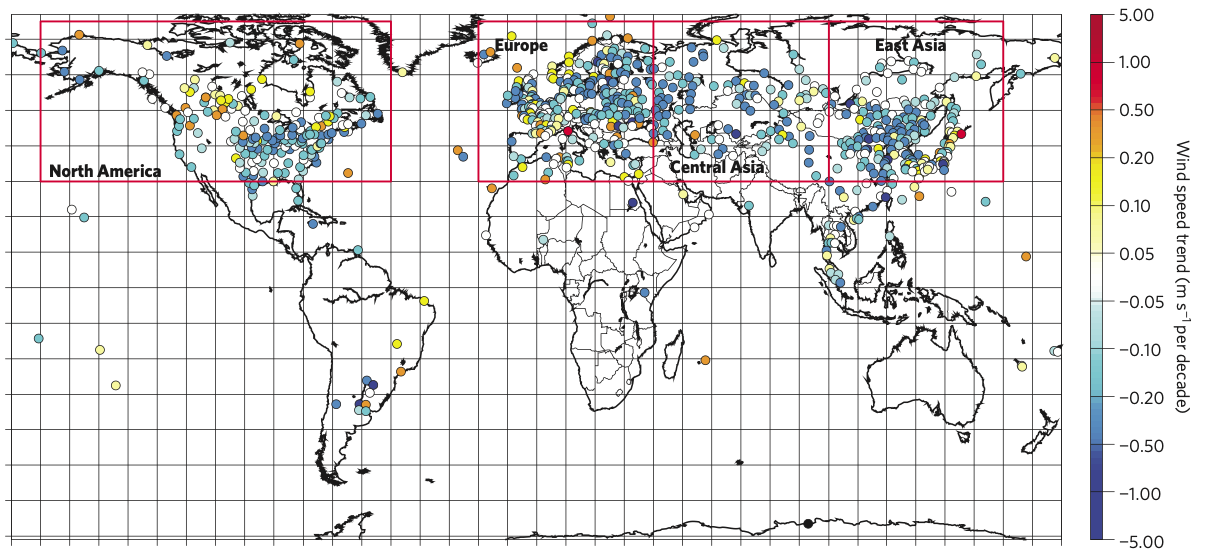
\includegraphics[width=1\textwidth]{北半球陆地地表风速趋势(Vautard等2010)}
    \bicaption{北半球陆地地表风速趋势。风速趋势使用1979-2008年地面观测计算得到。(来源:\citet{vautard2010northern})}{Land surface wind speed trends over the Northern Hemisphere. Wind speed trends were computed using surface observations from 1979 to 2016.(Source: \citet{vautard2010northern})}
    \label{fig:NHwindtrendVautard2010}
\end{figure}

\subsection{陆地地表风速长期变化的原因}

从动力学的角度,风速的变化满足下列关系:

\begin{equation} \label{eq:winddynmaic}
\frac{\mathrm{d} \vec{V}}{\mathrm{d} t} = \vec{G} + \vec{F} + \vec{g} + \vec{f}
\end{equation} ~\\
其中,$\vec{V}$为风矢量;$\vec{G} =\frac{1}{\rho} \nabla p $为气压梯度力,即为大气运动的驱动力,$\rho$ 为空气密度,$ p $为气压;$\vec{F} =-2 \Omega \times \vec{V} $为科里奥利力;$\vec{g}$ 为重力;$\vec{f}$为大气运动的阻力。由于科里奥利力和重力不会主动变化,因此,风速变化的可能原因可以分为两个方面:

\begin{enumerate}
 \item 大气运动驱动力的变化。大尺度的温度的变化会对大尺度大气运动驱动力产生影响,此外环流系统的变化也与大气运动驱动力变化密切联系。
 \item 大气运动阻力的变化。大气运动的阻力分为拖拽阻力和内部阻力,拖拽阻力主要由于城市化、植被变化等会引起地表粗糙度变化而产生;内部阻力主要则由于空气内部的湍流混合,与大气稳定度,风的垂直切变等有关。
\end{enumerate}

下面从主要从驱动力和阻力两个方面对前人研究进行回顾和总结:

\begin{enumerate}
\item 大气运动驱动力变化的影响

气温的不均匀变化可能会导致气压梯度力的变化,进而影响地表风速。\citet{klink1999trends}认为美国的地表风速变化可以由美国高纬度增温快于低纬度来解释。\citet{xu2006steady}认为冬季中国北部增温快于东边的西北太平洋,而夏季中国中部降温东边的西北太平洋增温,这使得东亚冬季风和夏季风均出现减弱,从而使得中国陆地地表风速减小。\citet{yan2002an}认为南半球变暖使得北大西洋风暴轴偏移,使得欧洲大陆风暴强度减小,从而使得欧洲陆地地表风速减小。

环流系统的变化会影响到地表风速。很多研究表明,北大西洋涛动(NAO)对欧洲陆地地表风速有显著影响\citep{beniston2005mountain, earl20131980–2010},而北极涛动(AO)与中国陆地地表风速有很好的相关\citep{chen2013wind}。此外,研究发现,厄尔尼诺南方涛动(ENSO)处于正为位相时,中国平均陆地地表风速相比ENSO负位相时高出55\%,表明ENSO对于中国陆地地表风速可能有影响\citep{chen2013wind}。\citet{wu2016estimating}发现,在东亚夏季风(EASM)强年,中国夏季陆地地表风速相比于EASM弱年高出$0.017 ~ m ~ s^{-1}$,表明了东亚夏季风可能影响中国陆地地表风速。近些年来,东亚季风有减弱的趋势\citep{zhu2012increases, ding2014interdecadal},也被认为是东亚陆地地表风速减小的原因之一\citep{xu2006steady}。

\begin{figure}[!htbp]
    \centering
    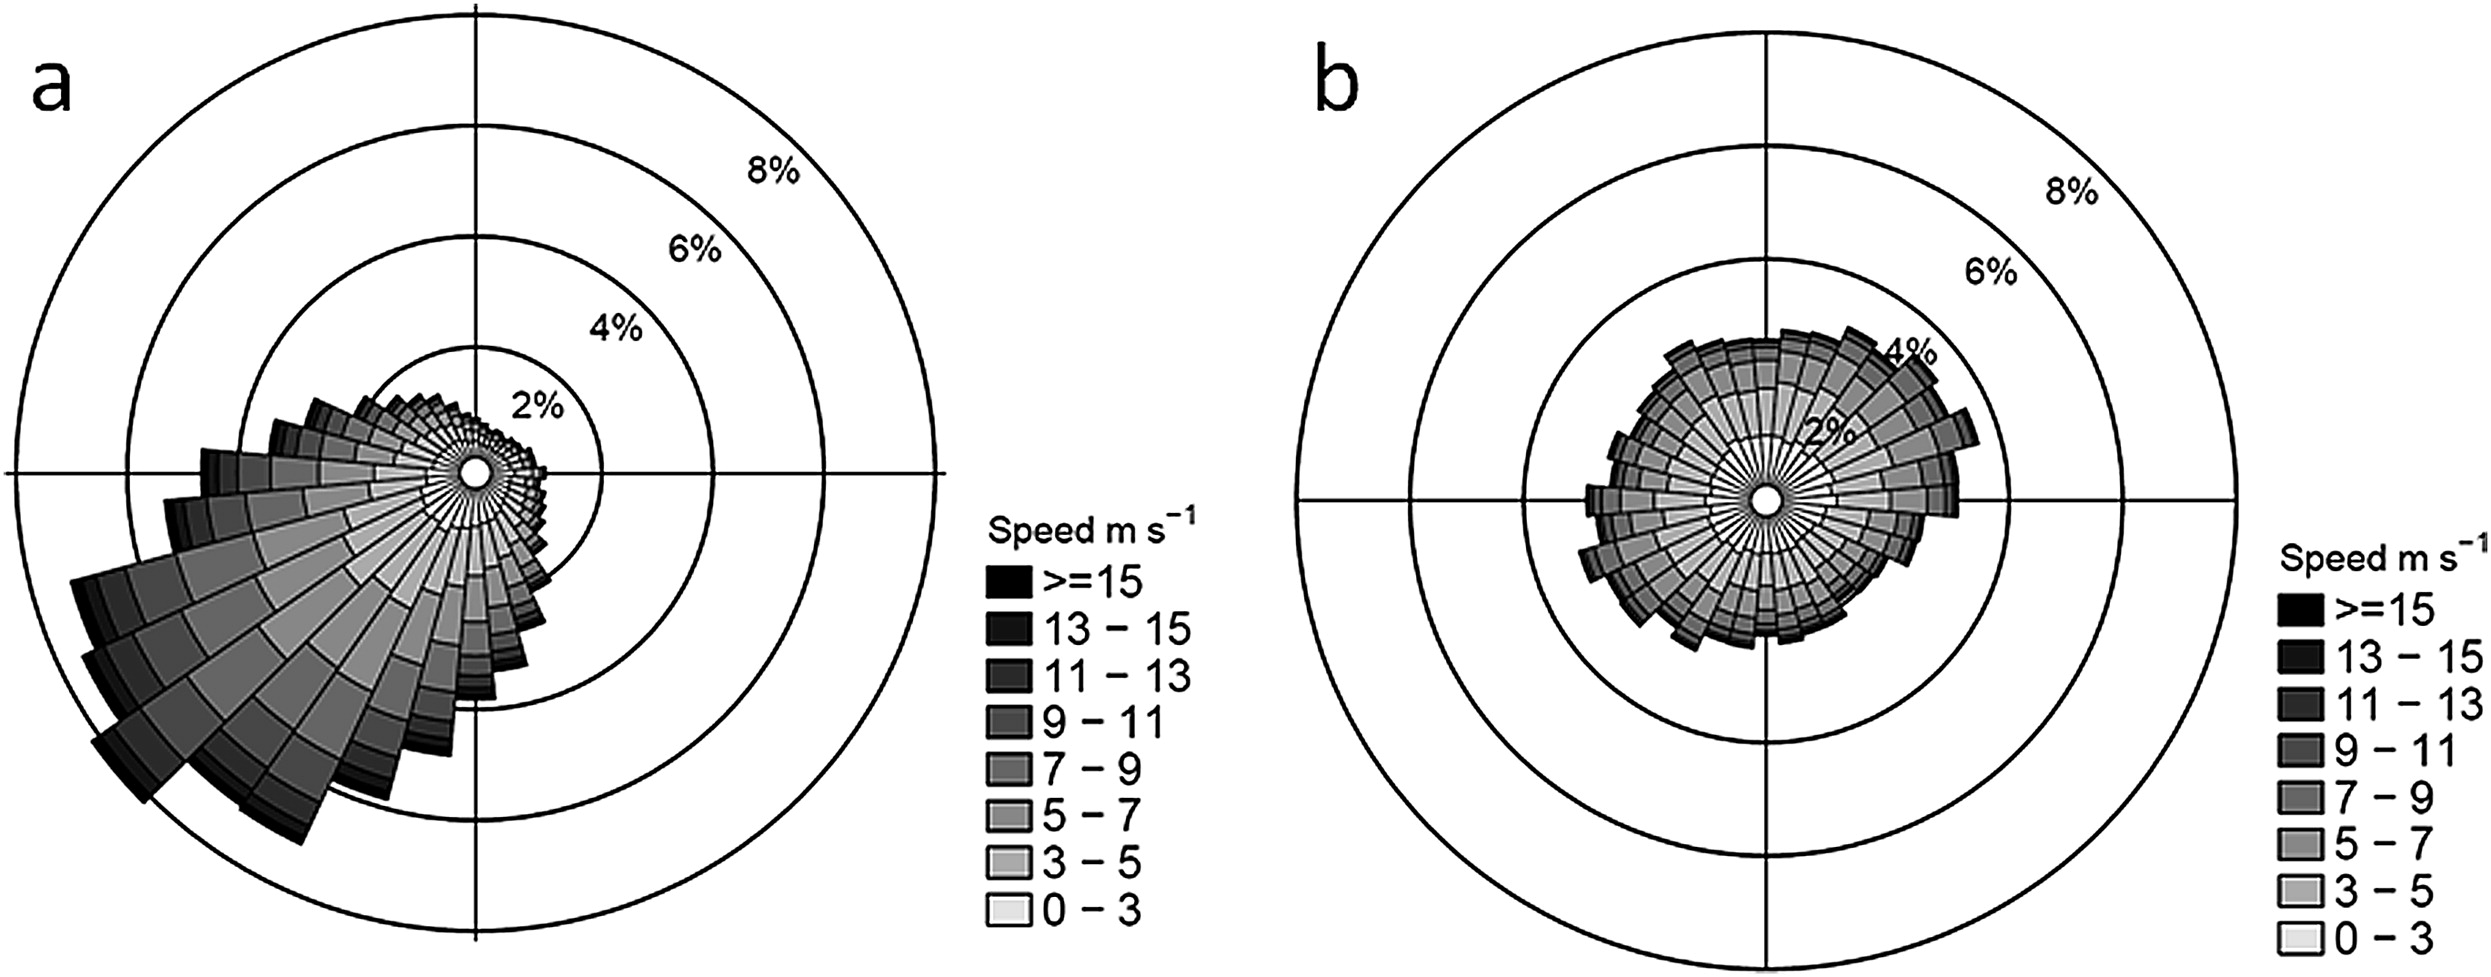
\includegraphics[width=1\textwidth]{英国地表风速与NAO(Earl等,2013)}
    \bicaption{不同NAO指数下的英国地表风。a)NAO指数大于2,b)NAO指数小于-2。(来源:\citet{earl20131980–2010})}{Surface winds over the United Kingdom under different NAO index. a)NAO index > 2, b)NAO index < -2. (Source: \citet{earl20131980–2010})}
    \label{fig:NAOUKwindEarl2013}
\end{figure}

\item 大气运动阻力变化的影响

如前文所述,观测陆地地表风速在近几十年来出现了显著减小,但海表风速却出现了增加\citep{tobin2014global, berrisford2015global, dunn2016surface},这从一定程度上反映了陆面拖拽阻力的变化对地表风速等影响。\citet{vautard2010northern}认为北半球陆地地表风速减弱的25\%–60\%可以由地表粗糙度变化解释。\citet{wever2012quantifying}发现欧洲地表粗糙度变化可以解释欧洲1981-2009年地表风速减弱的70\%。由于地表粗糙度观测数据的缺乏,地表粗糙度如何变化以及其对地表风速的影响难以直接考察,因而很多研究者采用了一些间接方式进行研究。例如,比较再分析资料(如NCEP/NCAR)与观测资料的差别来分析土地利用变化的影响\citep{kalnay2003impact, zha2017effects},比较城市与乡村站点风速变化来考察城市化的影响\citep{klaic2002modification, guo2011changes},也有利用数值试验来研究土地利用变化的影响\citep{vautard2010northern, zha2019numerical}。

\begin{figure}[!htbp]
    \centering
    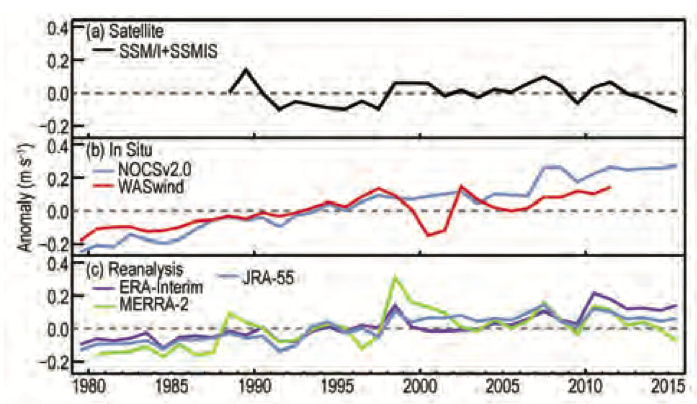
\includegraphics[width=0.9\textwidth]{海表风速变化(Dunn等,2016)}
    \bicaption{海表风速变化。a)卫星资料,b)观测资料,c)再分析资料。(来源:\citet{dunn2016surface})}{Changes in ocean surface winds. a) Satellite, b) In situ observation, c) Reanalysis. (Source: \citet{dunn2016surface})}
    \label{fig:Oceanwindchange}
\end{figure}

\begin{figure}[!htbp]
    \centering
    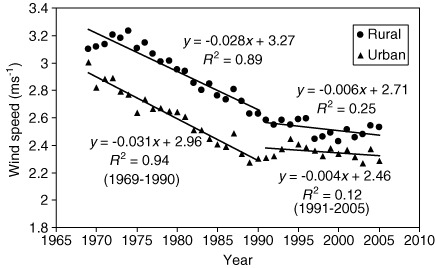
\includegraphics[width=0.95\textwidth]{中国城市化与风速变化(Guo等,2011)}
    \bicaption{中国城市与乡村风速变化,圆圈代表乡村站点风速,三角代表城市站点风速。(来源:\citet{guo2011changes})}{Wind speed evolution in urban and rural stations in China, circles denote rural station wind speeds, triangles denote urban station wind speeds . (Source: \citet{guo2011changes})}
    \label{fig:UrbanvsRuralChina}
\end{figure}

\begin{figure}[!htbp]
    \centering
    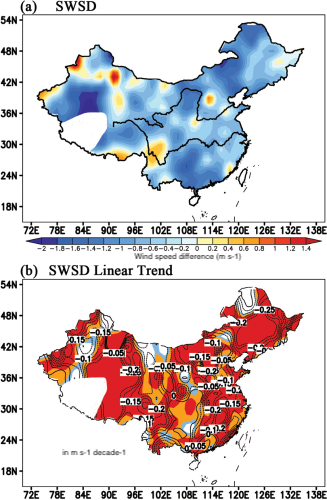
\includegraphics[width=0.85\textwidth]{中国地表风速OMR(Zha等,2017)}
    \bicaption{中国观测与再分析地表风速的差别。a)观测减ERA-Interim,b)观测减ERA-Interim的线性趋势。蓝色、黄色、红色区域分别代表显著性水平超过 90\%、95\%和99\%(来源:\citet{zha2017effects})}{Observations minus reanalysis surface wind speeds over China. a) Observation minus ERA-Interim, b) Linear trends of observation minus ERA-Interim. Blue, yellow, and red area denote that the significance levels outreach 90\%, 95\%, and 99\%, respectively. (Source: \citet{zha2017effects})}
    \label{fig:OMRchina}
\end{figure}


地表附近大气稳定度的变化会影响高层动量向下传递,从而影响地表风速。有研究表明,气溶胶和温室气体的变化可能改变大气稳定度\citep{ramanathan2005atmospheric, bichet2012causes}。气溶胶对于太阳辐射等吸收和反射会减少到达地面的短波辐射,从而增加大气稳定度。\citet{bichet2012causes}利用数值试验发现气溶胶增加使得印度和中国的地表风速分别减少了$ 0.13 ~ m ~ s^{-1}$和$0.03 ~ m ~ s^{-1}$。温室气体会使得不同层次的大气不均匀增温,从而改变大气的稳定度\citep{santer2011reproducibility}。\citet{bichet2012causes}的数值试验也探究了温室气体浓度对于地表风速的影响,但发现这种影响在1950年后并不显著。

\begin{figure}[!htbp]
    \centering
    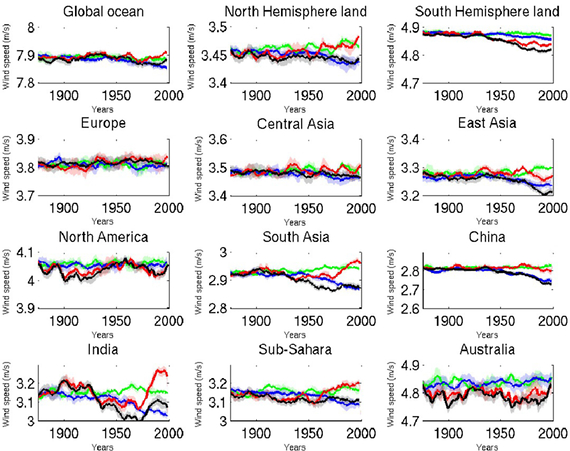
\includegraphics[width=1\textwidth]{外强迫对地表风速等影响(Bichet等,2012)}
    \bicaption{外强迫对地表风速等影响。黑线为控制试验,即包含所有外强迫,红线为气溶胶不变的情况,蓝线为海表温度保持不变的情况,绿色为气溶胶和海表温度均保持不变的情况(来源:\citet{bichet2012causes})}{Impact of external forcings on surface wind speed. Black line denotes control run, namely model run with all external forcings, red line denotes model run with aerosol remains unchanged, blue line denotes model run with sea surface temperature remains unchanged, and blue line denotes model run with aerosol and sea surface temperature remain unchanged. (Source: \citet{bichet2012causes})}
    \label{fig:ExternalForcing}
\end{figure}

\item 其他因素的影响

不可否认的是,一些人为因素同样会影响到观测的风速趋势,其中最主要的是观测仪器、规范以及观测环境的改变。\citet{mckee2000climate}指出,美国1990年左右安装的ASOS观测系统会使得大风风速相比之前的观测偏大,而小风风速偏小。\citet{刘学锋2012台站观测环境改变对我国近地面风速观测资料序列的影响}发现,台站障碍物视宽角对中国1971-2002年间地表风速趋势对贡献达到了1/3。

\end{enumerate}

\subsection{风能资源评估与变化}

\citet{archer2005evaluation}利用全球7753个地面观测站和446个探空观测站资料,计算了2000年全球的风能资源,发现风能资源总量相当于目前全球总用电量的约35倍,即约600 $PWh$。\citet{lu2009global}利用模拟的风场资料计算了2006年全球未被林地、冰川覆盖,城市以外地区的风能资源,发现其总量超过当年全球总用电量的200倍,全球总能源消耗的25倍。一些工作评估了未来气候变化对于风能资源的可能影响,\citet{pryor2011assessing}利用CMIP5全球气候模式未来情景预估,使用区域气候模式降尺度之后发现,美国的近地面风能资源没有显著变化。\citet{karnauskas2018southward}发现,在未来预估情景下,北半球中纬度风能资源会减小,而热带地区和南半球风能资源会增加。

\begin{figure}[!htbp]
    \centering
    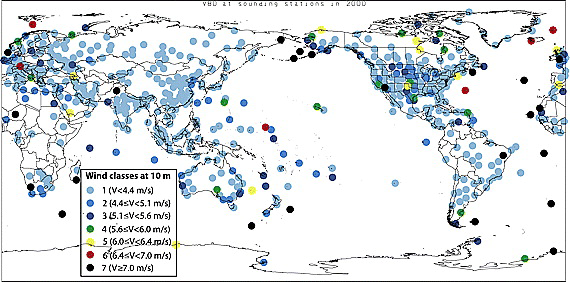
\includegraphics[width=1\textwidth]{风能资源分布(Archer和Jacobson,2005)}
    \bicaption{2000年风能资源分布。(来源:\citet{archer2005evaluation})}{Spatial distribution of wind energy resources in 2000. (Source: \citet{archer2005evaluation})}
    \label{fig:windenergyArcher2005}
\end{figure}

\section{论文主要内容}

从前面的回顾可以看出,陆地地表风速减弱是一个在全球普遍发生且颇为显著的现象,环流、温度、地表粗糙度等因素均可能对地表风速的变化产生影响。本文旨在于对大尺度陆地地表风速长期变化的相关问题做一个系统梳理,试图对以下问题作出回答:

\begin{enumerate}
\item 大尺度陆地地表风速的趋势,年代际变化有何特征?在不同区域,不同季节有何差别?
\item 大尺度陆地地表风速长期变化的背后的原因是什么?什么因素占主导作用?
\item 大尺度陆地地表风速长期变化对于风能资源有何影响?尤其对于风能资源较为丰富,有开发价值的地区的影响如何?
\end{enumerate}

由此,本文拟解决的主要科学问题如下:

\begin{enumerate}
\item 北半球陆地地表风速长期变化的时空特征

本文的分析主要以观测资料为基础,由于前期研究表明南半球高质量且长时间的地表风速序列较少,因而将主要研究区域选定为北半球。本文将北半球分为北美洲、欧洲、亚洲三个区域,对北半球总体状况和三个区域分别进行了分析,考察了陆地地表风速的长期趋势和年代际变化,以及在不同百分位,不同季节,不同高度的差别。由于仪器更换等人为误差的影响,观测地表风速长期变化存在不确定性,本文对比观测与多套再分析资料分析了这种不确定性。

\item 北半球陆地地表风速变化的机理

如前文所述,陆地地表风速变化的原因主要分为大气运动驱动力的变化和大气运动阻力的变化。本文从这两个方面出发,全面考察这两类变化的影响,包括海平面气压场、环流系统、大尺度海温、城市化、植被变化、大气稳定度等。

\item 北半球陆地地表风速长期变化对风能资源的影响

本文利用地面观测资料首先分析了北半球近38年来的风能资源整体状况,并筛选出了适于进行风能资源开发的地区,然后分析了陆地地表风速长期变化对风能资源的影响,特别是对于适于风能资源开发地区的影响。另外分析了全球气候模式对风能资源长期变化的模拟能力,以此作为评估全球气候模式风能资源预估可靠性的参考。

\end{enumerate}

论文章节安排如下:

第1章	\quad 绪论

第2章	\quad 北半球陆地地表风速长期变化的时空特征

第3章	\quad 大气运动驱动力变化对陆地地表风速长期变化的影响

第4章	\quad 大气运动阻力变化对陆地地表风速长期变化的影响

第5章	\quad 北半球陆地地表风速长期变化对风能资源的影响

第6章	\quad 总结与展望

%%  --------------------- chapter 2--------------------- %
\chapter{北半球陆地地表风速长期变化的时空特征}\label{chap:SpatiotemporalCharacteristics}

\section{引言}

如第\ref{chap:intro}章所述,近几十年来,全球陆地地表风速出现了普遍下降,平均趋势约为$-0.08 ~ m ~ s^{-1}$ 每十年(参见表  \ref{tab:globalwindtrend})。同时,不同区域的风速长期趋势又有显著的差别,例如,中国在1971-2008年平均风速趋势为$ -0.12 ~ m ~ s^{-1} $ 每十年\citep{yin2010determining},而印度在1971-2002年平均风速趋势却达到了$ -0.27 ~ m ~ s^{-1}$ 每十年 \citep{mcvicar2012global}。此外,同一区域不同时间段的趋势也可能会有差别,例如,西班牙在1961-2001年间平均风速趋势为$ -0.014 ~ m ~ s^{-1}$每十年,而在1979-2008年间平均风速趋势为$ -0.006 ~ m ~ s^{-1}$ 每十年\citep{azorinmolina2014homogenization}。不同季节间的风速趋势差别可能同样不可忽略,例如,韩国1954-2003年间风速变化最快的季节为春季,达到 $-0.19 ~ m ~ s^{-1}$每十年,而变化最慢的季节为夏季,为$-0.10 ~ m ~ s^{-1}$ 每十年 \citep{kim2015recent}。因而,为了对北半球陆地地表风速长期变化有完整的把握,本章将全面考察不同区域,不同年代和不同季节的状况。

长时间的气候资料会不可避免的受各种人为因素的影响,出现不均一的情况。通常,处理这种序列不均一的方法有两种:第一是通过严格的质量控制,剔除不均一的站点\citep{vautard2010northern, zeng2019a};另一种是通过均一化方法,将本来不均一的序列变为均一的序列\citep{wan2010homogenization, azorinmolina2014homogenization}。第一种方法通常会使得可以用于分析的观测序列大大减少,但保存了原始观测序列的信息;第二种方法能最大限度的保持观测序列的数量,但均一化方法本身依赖于一系列假设条件和高质量的参考序列,在实际操作中很难被满足,因而均一化过程本身的不确定性也不可忽略。本章内容使用了第一种方法来降低观测序列的不均一性对分析结果的影响。另外,再分析资料相对观测资料有更好的均一性,本章使用了多套再分析资料风场与观测资料进行对比来评估风速长期变化的不确定性。

\section{资料和方法}

本章中使用了以下2套地面观测数据:

\begin{enumerate}
\item NCEI-ISD数据集\citep{smith2011the}由美国大气海洋局(NOAA)制作,包含从全球超过100个数据源获得的小时地面观测资料,总共有超过35000个站点,其中14000个站点目前在每日上传数据。此数据集本身通过54种质量控制算法进行检测,包括有效性检验、极端值检验、内部一致性检验(与本站同一种观测数据进行比较)和外部一致性检验(与本站其他观测数据进行比较)。本章选取了1979-2016年地表风速数据进行研究,为了保证数据质量,另外增加了以下数据质量控制步骤:
\begin{enumerate}
\item 剔除站点水平迁移超过0.02度(约2 km)或垂直迁移超过20 m的站点。
\item 剔除未通过NCEI-ISD质量控制的数据,将剩余数据处理成日平均值。
\item 剔除存在较多缺测站点:首先,剔除一年中数据少于360天的年份;然后,剔除缺测年份多于序列长度10\%的站点(本研究序列长度为38年,即剔除缺测超过3年的站点)。
\end{enumerate}
\item 中国地面气候资料日值数据集(V3.0) 由中国气象数据服务中心(CMDC)制作,包含824个地面观测站点。此数据集进行了多项质量控制,包括极端值检验,内部一致性检验,外部一致性检验和人工检查。本章选取了1979-2016年地表风速数据,为了保证数据质量,进行了额外的质量控制步骤,方法与NCEI-ISD类似。
经过严格质量控制后,NCEI-ISD剩余785个站点序列,中国地面气候资料日值数据集(V3.0)剩余351个站点序列。NCEI-ISD原本包含了中国的站点,然而中国参与国际交换的站点仅有194个,所以使用中国地面气候资料日值数据集(V3.0)对中国地面观测序列进行补充。一致性检验表明两套数据在中国地表风速有较好的一致性。将两套数据合并,剔除掉98个重复的站点,形成一套包含全球1038个站点的高质量风速数据,命名为NCEI-CMDC集合数据集。本章\ref{sec:NHwindchange}节中所有的分析均是基于这套数据。由于这要数据所包括的站点超过90\%坐落于北半球,因而对于这套数据中对所有站点的分析主要体现的是北半球的状况。
\end{enumerate}

本章中使用了以下5套再分析数据集与观测数据进行对比:

\begin{enumerate}
\item NCEP/NCAR再分析资料\citep{kalnay1996the}的水平分辨率为$2.5 \times 2.5$度,有28个垂直层次。其地表粗糙度的数据不随时间变化,且陆地地表风速未被同化,10 m风速是由模式最底层的风速根据Monin-Obukhov相似理论外插得到。NCEP/NCAR使用的模式在近地面100 hPa内有5个垂直层次,最底层为$\sigma = 0.995$。本章研究使用了6小时分辨率10 m U、V风场资料。
\item NCEP-DOE再分析资料\citep{kanamitsu2002ncep–doe}的水平分辨率为$1.9 \times 1.9$度,垂直层次与NCEP/NCAR相同,为28个。其同化的数据也与NCEP/NCAR一致,只是算法上有所改进。与地表风速相关的改进包括地形平滑和边界层参数化方案以及土壤湿度的参数化。10 m风速的获得与NCEP/NCAR一致。本章研究使用了6小时分辨率10 m U、V风场资料。
\item ERA-Interim再分析资料\citep{dee2011the}的水平分辨率为$ 0.75 \times 0.75$ 度,60个垂直层次。其同化了海表风速,但没有同化陆地地表风速。10 m风速同样是由模式最底层的风速根据Monin-Obukhov相似理论外插得到。本章使用了6小时分辨率10 m U、V风场资料。
\item MERRA-2再分析资料\citep{molod2014development}的水平分辨率为0.5纬度$\times$ 0.625经度,72个垂直层次 。其同化了海表风速,但没有同化陆地地表风速。10 m风速的计算方式与前面提到的几套再分析资料类似。本章使用了1小时分辨率10 m U、V风场资料。
\item JRA-55再分析资料\citep{kobayashi2015the}的水平分辨率为$ 1.25 \times 1.25$度,60个垂直层次。JRA-55同化了陆地地表风速资料,但仅用于近地面层(screen level)的分析,不会用于大气模式。10 m风速的由模式最底层风速根据单变量二维最优差值得到。本章使用了6小时分辨率10 m U、V风场资料。
\end{enumerate}

本章中线性趋势的计算使用基于最小二乘方法的线性回归,计算方法如下:

建立线性回归模型:
\begin{equation} \label{eq:linearregression}
y = \beta_{0} + \beta_{1}x + \varepsilon
\end{equation} 
其中$\beta_{0}$和$\beta_{1}$为回归系数($\beta_{1}$即为“趋势”),$x$为回归量,$y$为回归子, $\varepsilon$为残差,为使得残差平方和最小,
\begin{equation} 
 \pmb{\beta} = \left( X^{T}X \right)^{-1} X^{T} Y 
\end{equation} 
$X$为回归量矩阵,$ \pmb{\beta} $为回归系数向量,$Y$为回归子向量。

统计显著性检验使用双侧t检验。突变点检测使用滑动t检验,人为设置某一时刻为基准点,t统计量计算方法为:

\begin{equation} \label{eq:mvttest}
t = \frac{\bar{x_{1}} - \bar{x_{2}}}{ s \sqrt{\frac{1}{n_{1}} + \frac{1}{n_{2}}}}
\end{equation} 
其中,
\begin{equation} 
s = \sqrt{\frac{n_{1}\sigma_{1}^{2} + n_{2}\sigma_{2}^{2}}{n_{1} - n_{2} - 2}}
\end{equation} ~\\
$\bar{x_{1}}$、$\bar{x_{2}}$分别为基准点前后子序列均值,$\sigma_{1}$ 、$\sigma_{2}$  为子序列标准差,$n_{1}$ 、$n_{2}$为子序列样本数量,对比$t$统计量与$t$分布临界值大小确定突变点的显著性水平。

\section{北半球陆地地表风速长期线性趋势}\label{sec:NHwindchange}

\subsection{陆地地表风速长期线性趋势的空间特征}

\begin{figure}[!b]
    \centering
    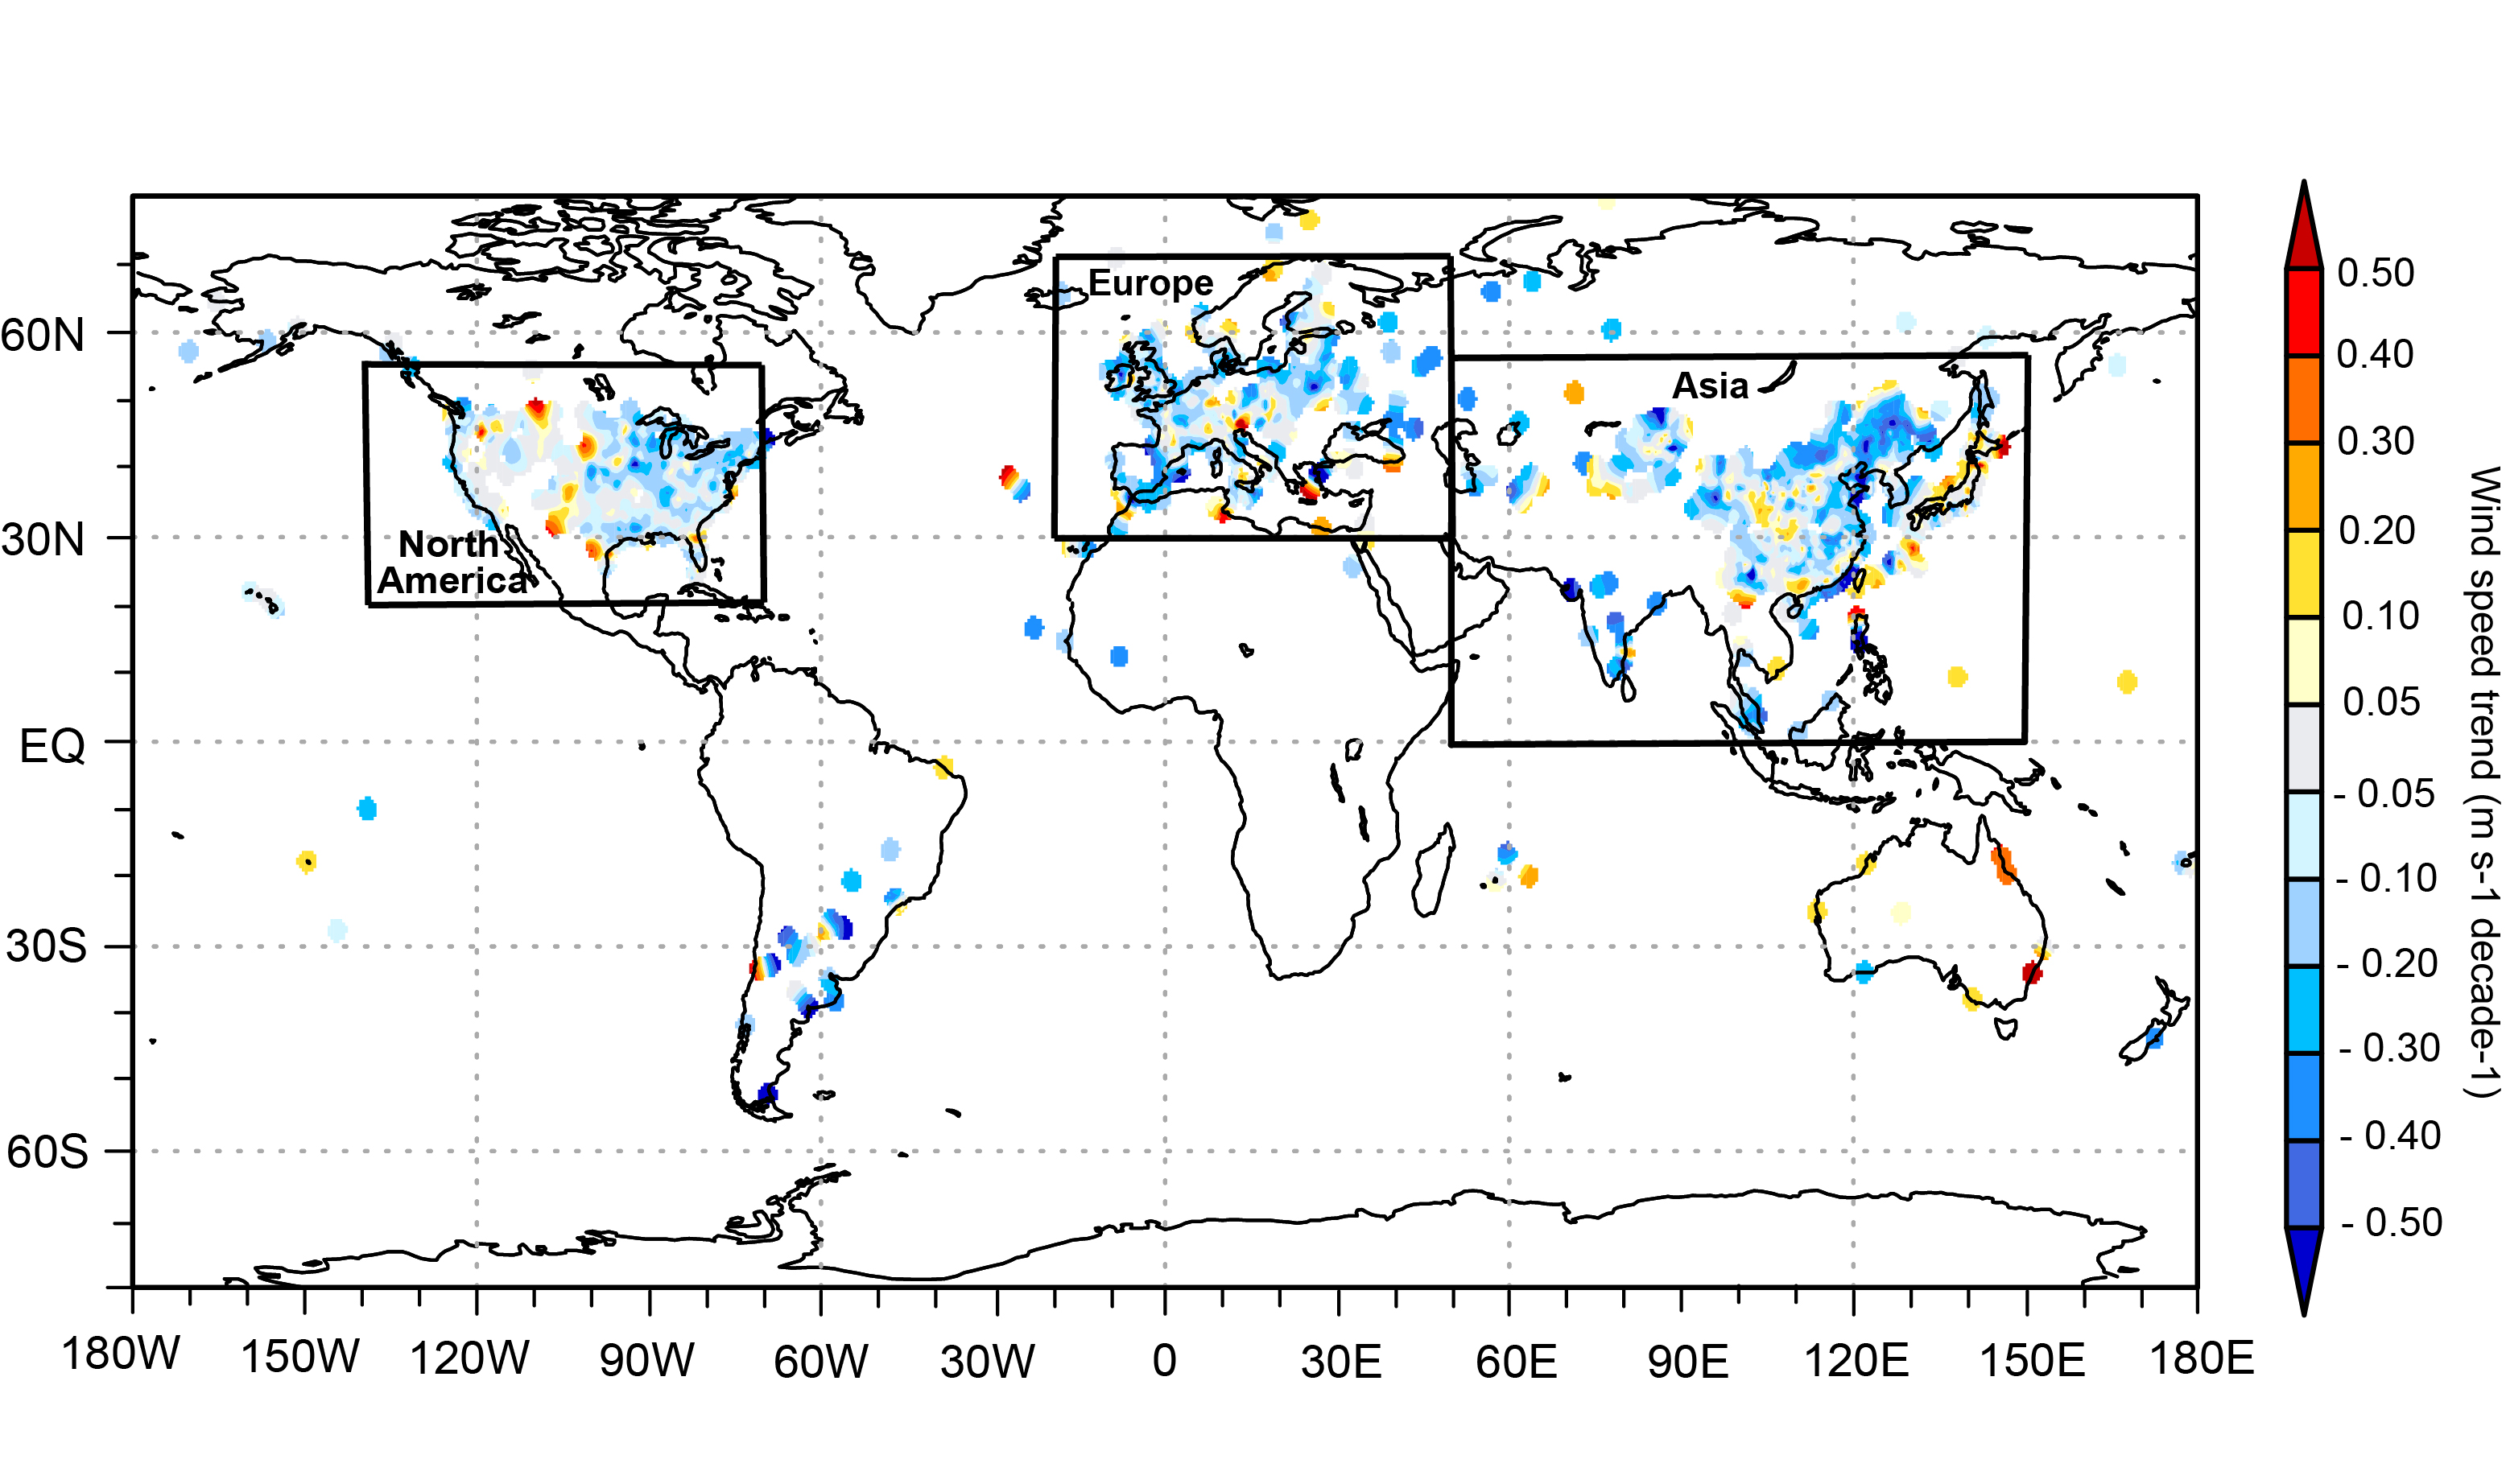
\includegraphics[width=1\textwidth]{全球年平均风速长期趋势}
    \bicaption{全球年平均风速长期趋势($m ~ s^{-1}$每十年)。图中三个框出的区域的范围分别为:北美洲 20-55 N,50-140 W;欧洲 30-70N,20W-50E;亚洲0-55N,50-150E。}{Long-term linear trends of annual mean wind speed across the globe (in $m ~ s^{-1} ~ decade^{-1}$). The spatial ranges of the framed areas are North America 20-55 N, 50-140 W, Europe 30-70N, 20W-50E, Asia 0-55N, 50-150E. }
    \label{fig:NHwindtrend}
\end{figure}

对NCEI-CMDC地表风速的年平均值进行线性回归,得到全球(主要是北半球)1979-2016年陆地地表风速的长期趋势。结果发现,全球有73\%的站点风速出现了下降趋势,其中有67\%显著下降(p < 0.01),中位数风速趋势为$ -0.081 ~ m ~ s^{-1}$每十年。将大部分观测站点分布的北半球分为三个区域:北美洲(20 - 55 N,50 - 140 W),欧洲(30 - 70 N,20 W - 50 E)和亚洲(0 - 55 N,50 - 150 E)分别进行分析,得到这三个地区中位数风速趋势分别为-0.075,-0.105和-0.075 $m ~ s^{-}$1每十年,即在38年中分别累计变化了-6.5\%,-9.6\%和-11.2\%。值得一提的是,中国的中位数风速趋势为-0.110 $m ~ s^{-1}$每十年,累计变化-17.5\%(图 \ref{fig:NHwindtrend})。这些结果与前人的研究具有较高的一致性(第\ref{chap:intro}章\;表 \ref{tab:globalwindtrend})。这里使用中位数而不是平均数,因为中位数相比平均数具有更好的鲁棒性,即更不容易受到极端值的影响,因而更适合于反映一个区域整体的状况,以下的许多分析也是基于中位数来进行。

\begin{figure}[!b]
    \centering
    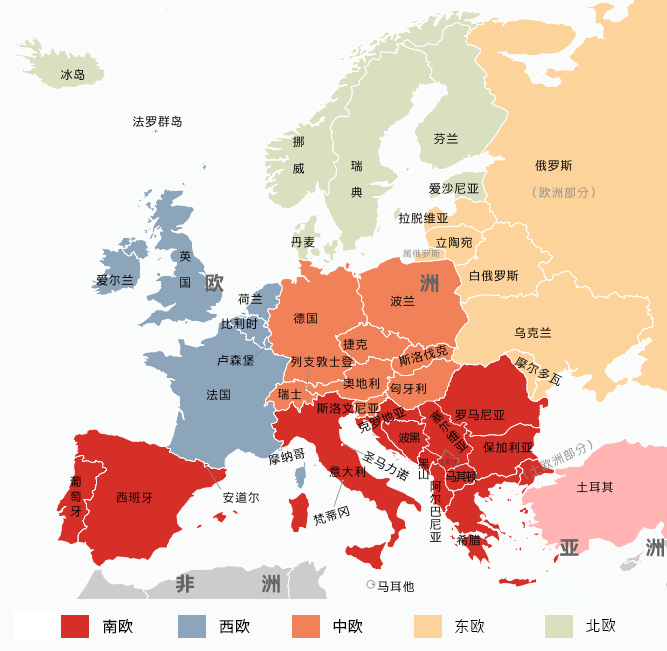
\includegraphics[width=0.6\textwidth]{欧洲分区}
    \bicaption{欧洲分区图}{European Zoning Map}
    \label{fig:EU}
\end{figure}

不同地区的地表风速长期趋势表现出了较大的差别。在北美洲,美国中北和东北地区风速下降最为明显,大部分站点趋势值小于-0.1 $m ~ s^{-1}$每十年;与之相对的,美国落基山脉地区多数站点风速趋势接近为0,个别站点出现了风速增强的情况;美国西海岸一线表现出了一定程度的风速下降,多数站点在-0.2 \textasciitilde -0.05 $m ~ s^{-1}$每十年。在欧洲,西欧地区(欧洲分区见图 \ref{fig:EU})有较为明显的风速下降;中欧地区,奥地利和斯洛文尼亚有较为明显风速上升,波兰中部风速有较为明显的下降,其他大部分地区没有明显的风速趋势;南欧地区,西班牙和葡萄牙风速有明显的上升;东欧地区大部分站点都表现了较为明显的风速下降。亚洲地区,印度风速下降明显,大部分站点趋势值小于-0.2 $m ~ s^{-1}$每十年;中国风速下降明显的地区是中国东北、华北和西北地区,中部地区部分站点风速有一定程度上升;日本风速部分站点风速明显下降,部分站点风速明显上升,二者数量大致相同(图 \ref{fig:NHwindtrend})。

\subsection{百分位风速长期线性趋势}

\begin{figure}[!b]
    \centering
    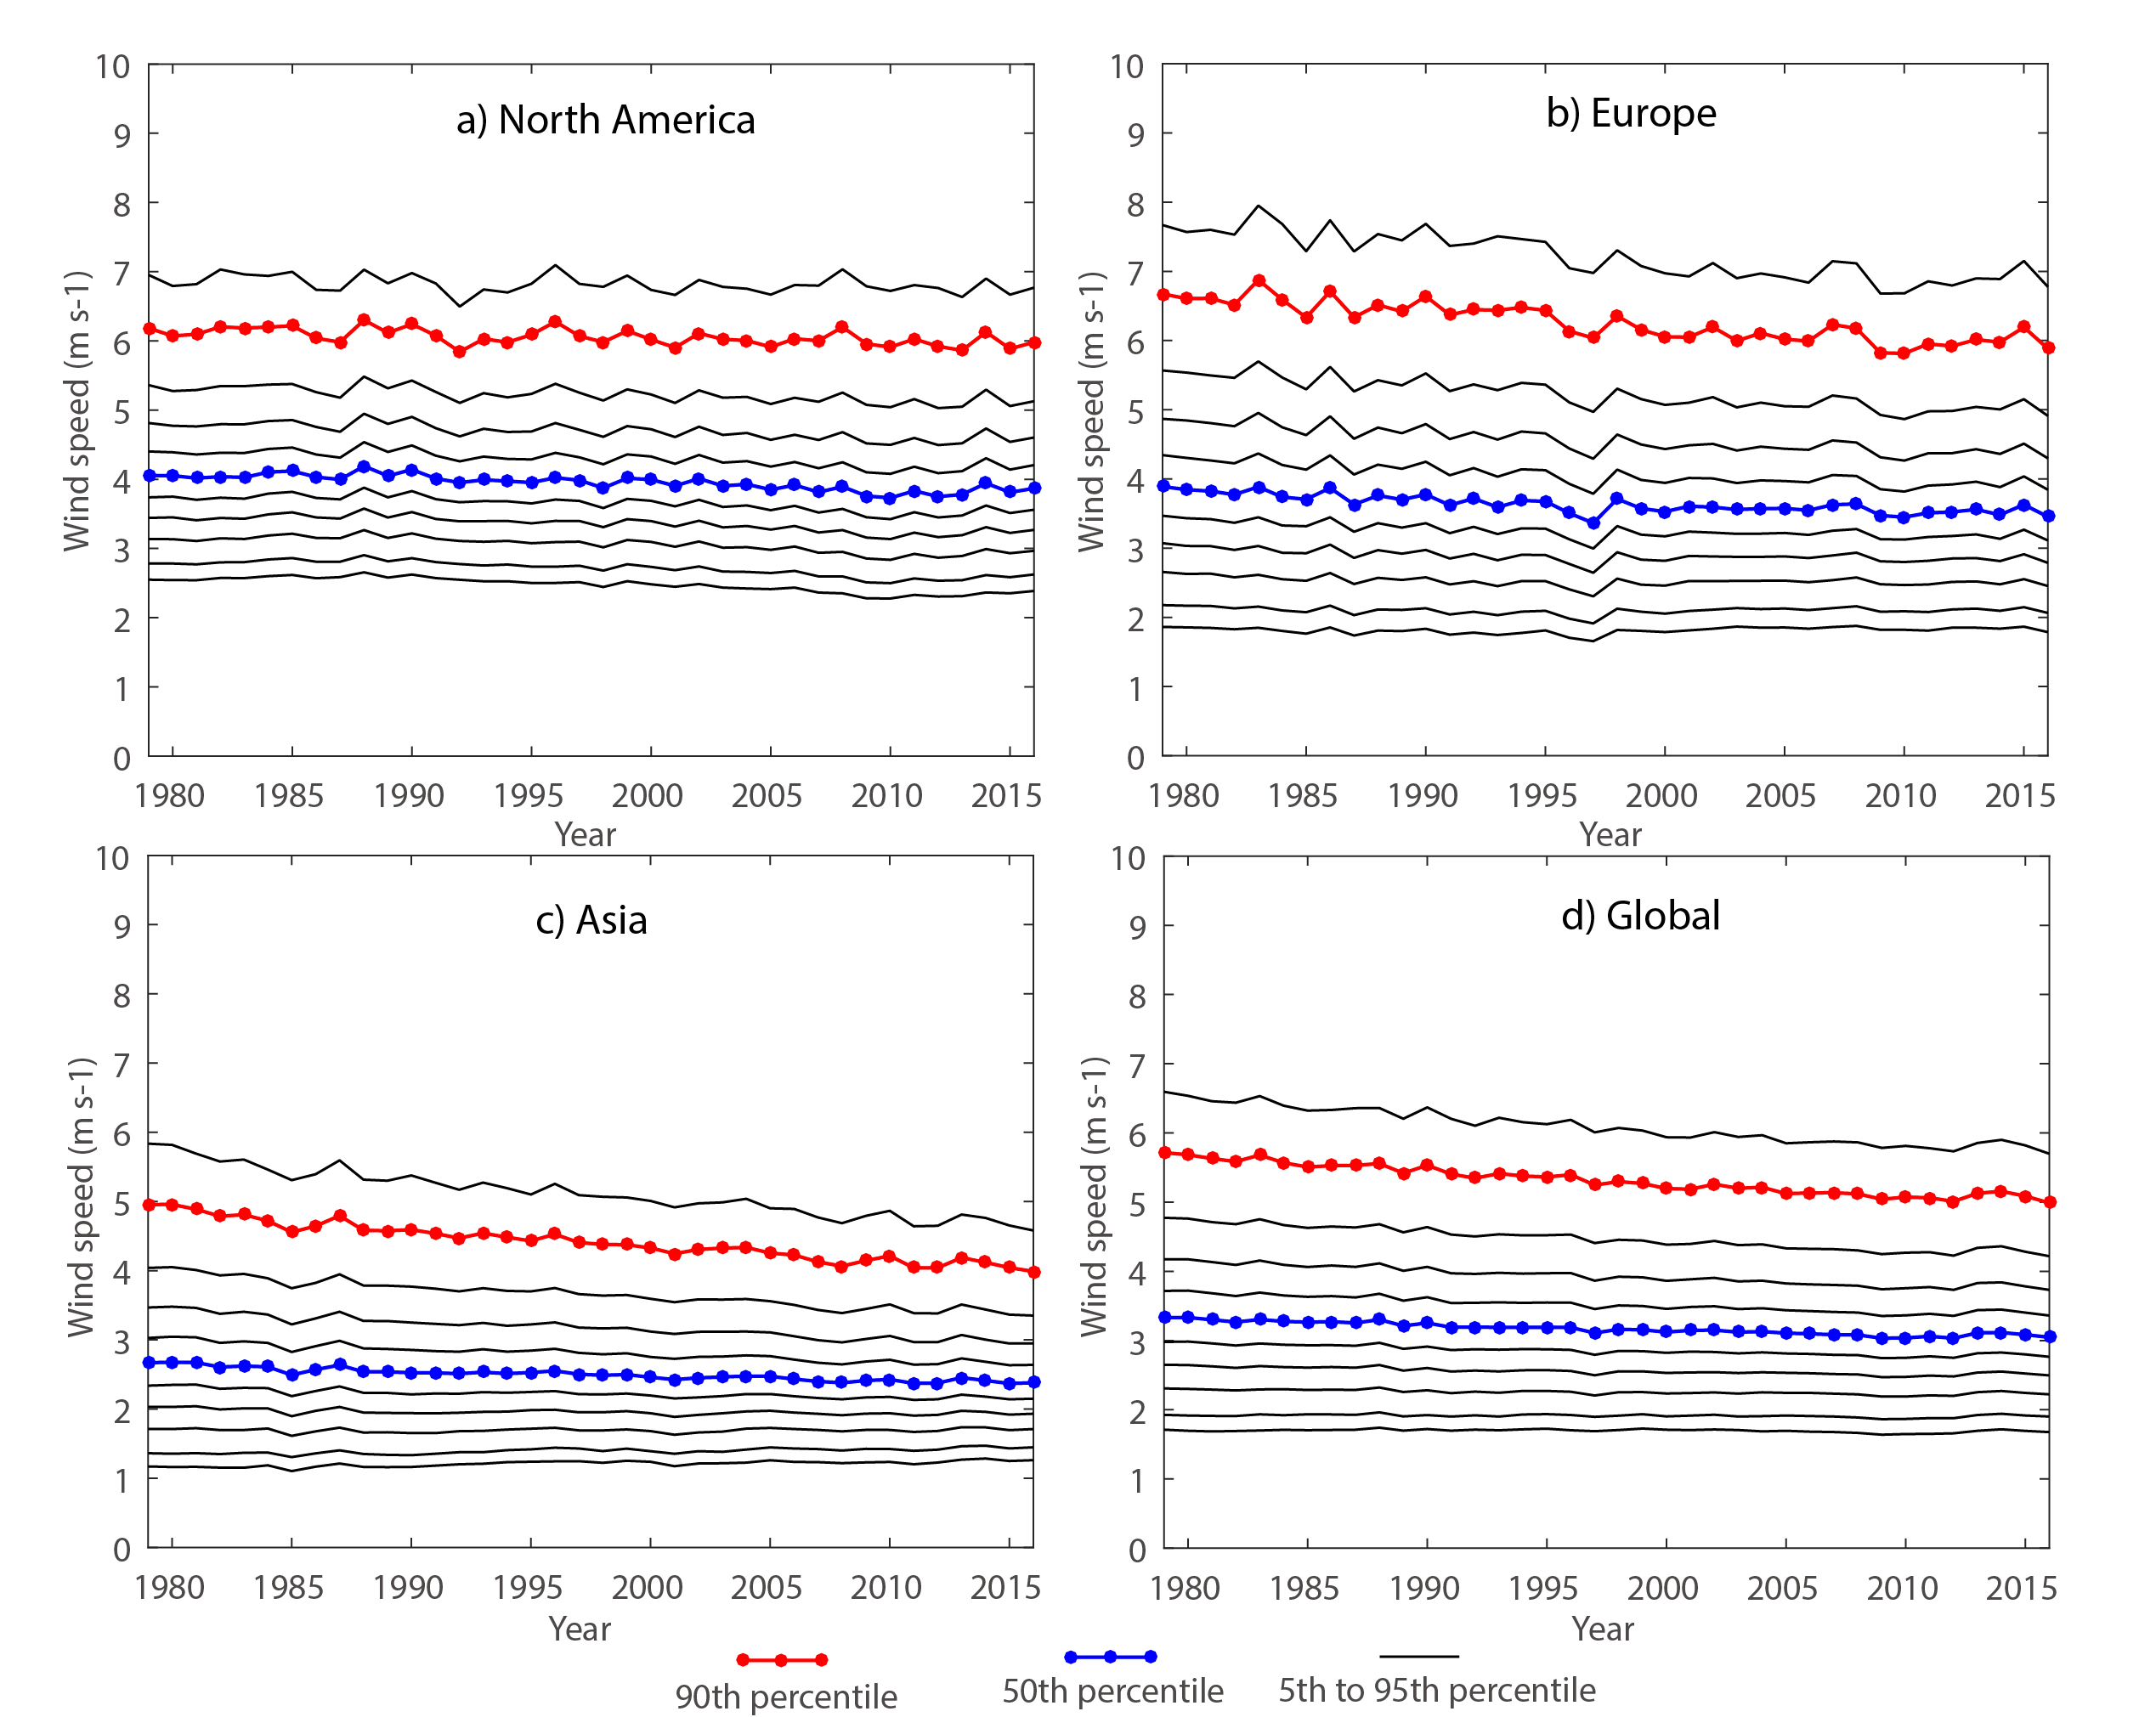
\includegraphics[width=1\textwidth]{百分位风速的演变}
    \bicaption{百分位风速的演变($m ~ s^{-1}$)。a)北美洲,b)欧洲,c)亚洲,d)全球。红色为90百分位,蓝色为50百分位,黑色为5、10、20、...、80、90、95百分位。}{Evolution of wind speeds at different percentiles (in $m ~ s^{-1}$). a) North America, b)Europe, c)Asia, d)Global. Red line denotes winds at 90 percentile, blue denotes 50 percentile, black denotes 5, 10, 20, ..., 80, 90, 95 percentile.}
    \label{fig:windpercentile}
\end{figure}

不同百分位风速变化也有不同特点。全球平均来看,大风下降快于小风(图 \ref{fig:windpercentile} d),表 \ref{tab:windpercentile})。各大洲分别来看,在北美洲,低百分位风速(即小风)下降快于高百分位风速(即大风)。5 - 40百分位风速的趋势约为-0.083 $m ~ s^{-1}$每十年,而80百分位风速趋势为-0.072 $m ~ s^{-1}$每十年,95百分位仅为-0.04 $m ~ s^{-1}$每十年。其中有部分原因可能是美国1990年代安装的ASOS观测系统测量的大风比之前观测系统偏大,而小风偏小\citep{mckee2000climate}。然而,在北美百分位风速演变中并未看到1990年代各百分位有显著变化,说明观测仪器变化的影响不是非常明显(图 \ref{fig:windpercentile} a),表 \ref{tab:windpercentile})。在欧洲,风速越大越趋向于减弱。5百分位风速略有上升,为0.008 $m ~ s^{-1}$每十年,从10百分位开始风速出现下降,到50百分位趋势达到了-0.093 $m ~ s^{-1}$每十年,90百分位下降速度超过了50百分位的两倍,达到了-0.218 $m ~ s^{-1}$每十年(图 \ref{fig:windpercentile} b),表 \ref{tab:windpercentile})。亚洲的情况与北美洲类似,5 – 20 百分位风速略有上升趋势,而从30百分位开始风速开始下降,50百分位趋势达到-0.074 $m ~ s^{-1}$每十年,90百分位达到-0.237 $m ~s^{-1}$每十年(图 \ref{fig:windpercentile} c),表 \ref{tab:windpercentile})。因为风力发电机只可以利用较大的风速进行,通常需超过3 $m ~s^{-1}$,因而在欧洲和亚洲出现的大风减弱更快的状况对风力发电十分不利。


\begin{table}[!htbp]
    \bicaption{全球及各大洲百分位风速趋势($m ~ s^{-1}$每十年)}{Global and regional wind speed trends at different percentiles (in $m ~ s^{-1} ~ decade^{-1}$) }
    \label{tab:windpercentile}
    \centering
    \small% fontsize
    \setlength{\tabcolsep}{15 pt}% column separation
    \renewcommand{\arraystretch}{1.0}%row space 
    \begin{tabular}{lcccc}
        \hline
        地区 & 北美洲 & 欧洲 & 亚洲 & 全球 \\
        %\cline{2-9}% partial hline from column i to column j
        \hline
        5th & -0.084 & 0.080 & 0.028 & -0.010 \\
        10th & -0.084 & -0.006 & 0.027 & -0.008 \\
        20th & -0.083 & -0.028 & 0.003 & -0.023 \\
        30th & -0.082 & -0.049 & -0.021 & -0.040 \\
        40th & -0.082 & -0.071 & -0.047 & -0.057 \\
        50th & -0.082 & -0.093 & -0.074 & -0.076 \\
        60th & -0.081 & -0.114 & -0.101 & -0.095 \\
        70th & -0.078 &  -0.141 & -0.134 & -0.118 \\
        80th & -0.072 & -0.171 & -0.174 & -0.177 \\
        90th & -0.057 & -0.218 & -0.237 & -0.184 \\
        95th & -0.040 & -0.261 & -0.296 & -0.222 \\           
        \hline
    \end{tabular}
\end{table}

\subsection{四季风速长期线性趋势}

\begin{figure}[!b]
    \centering
    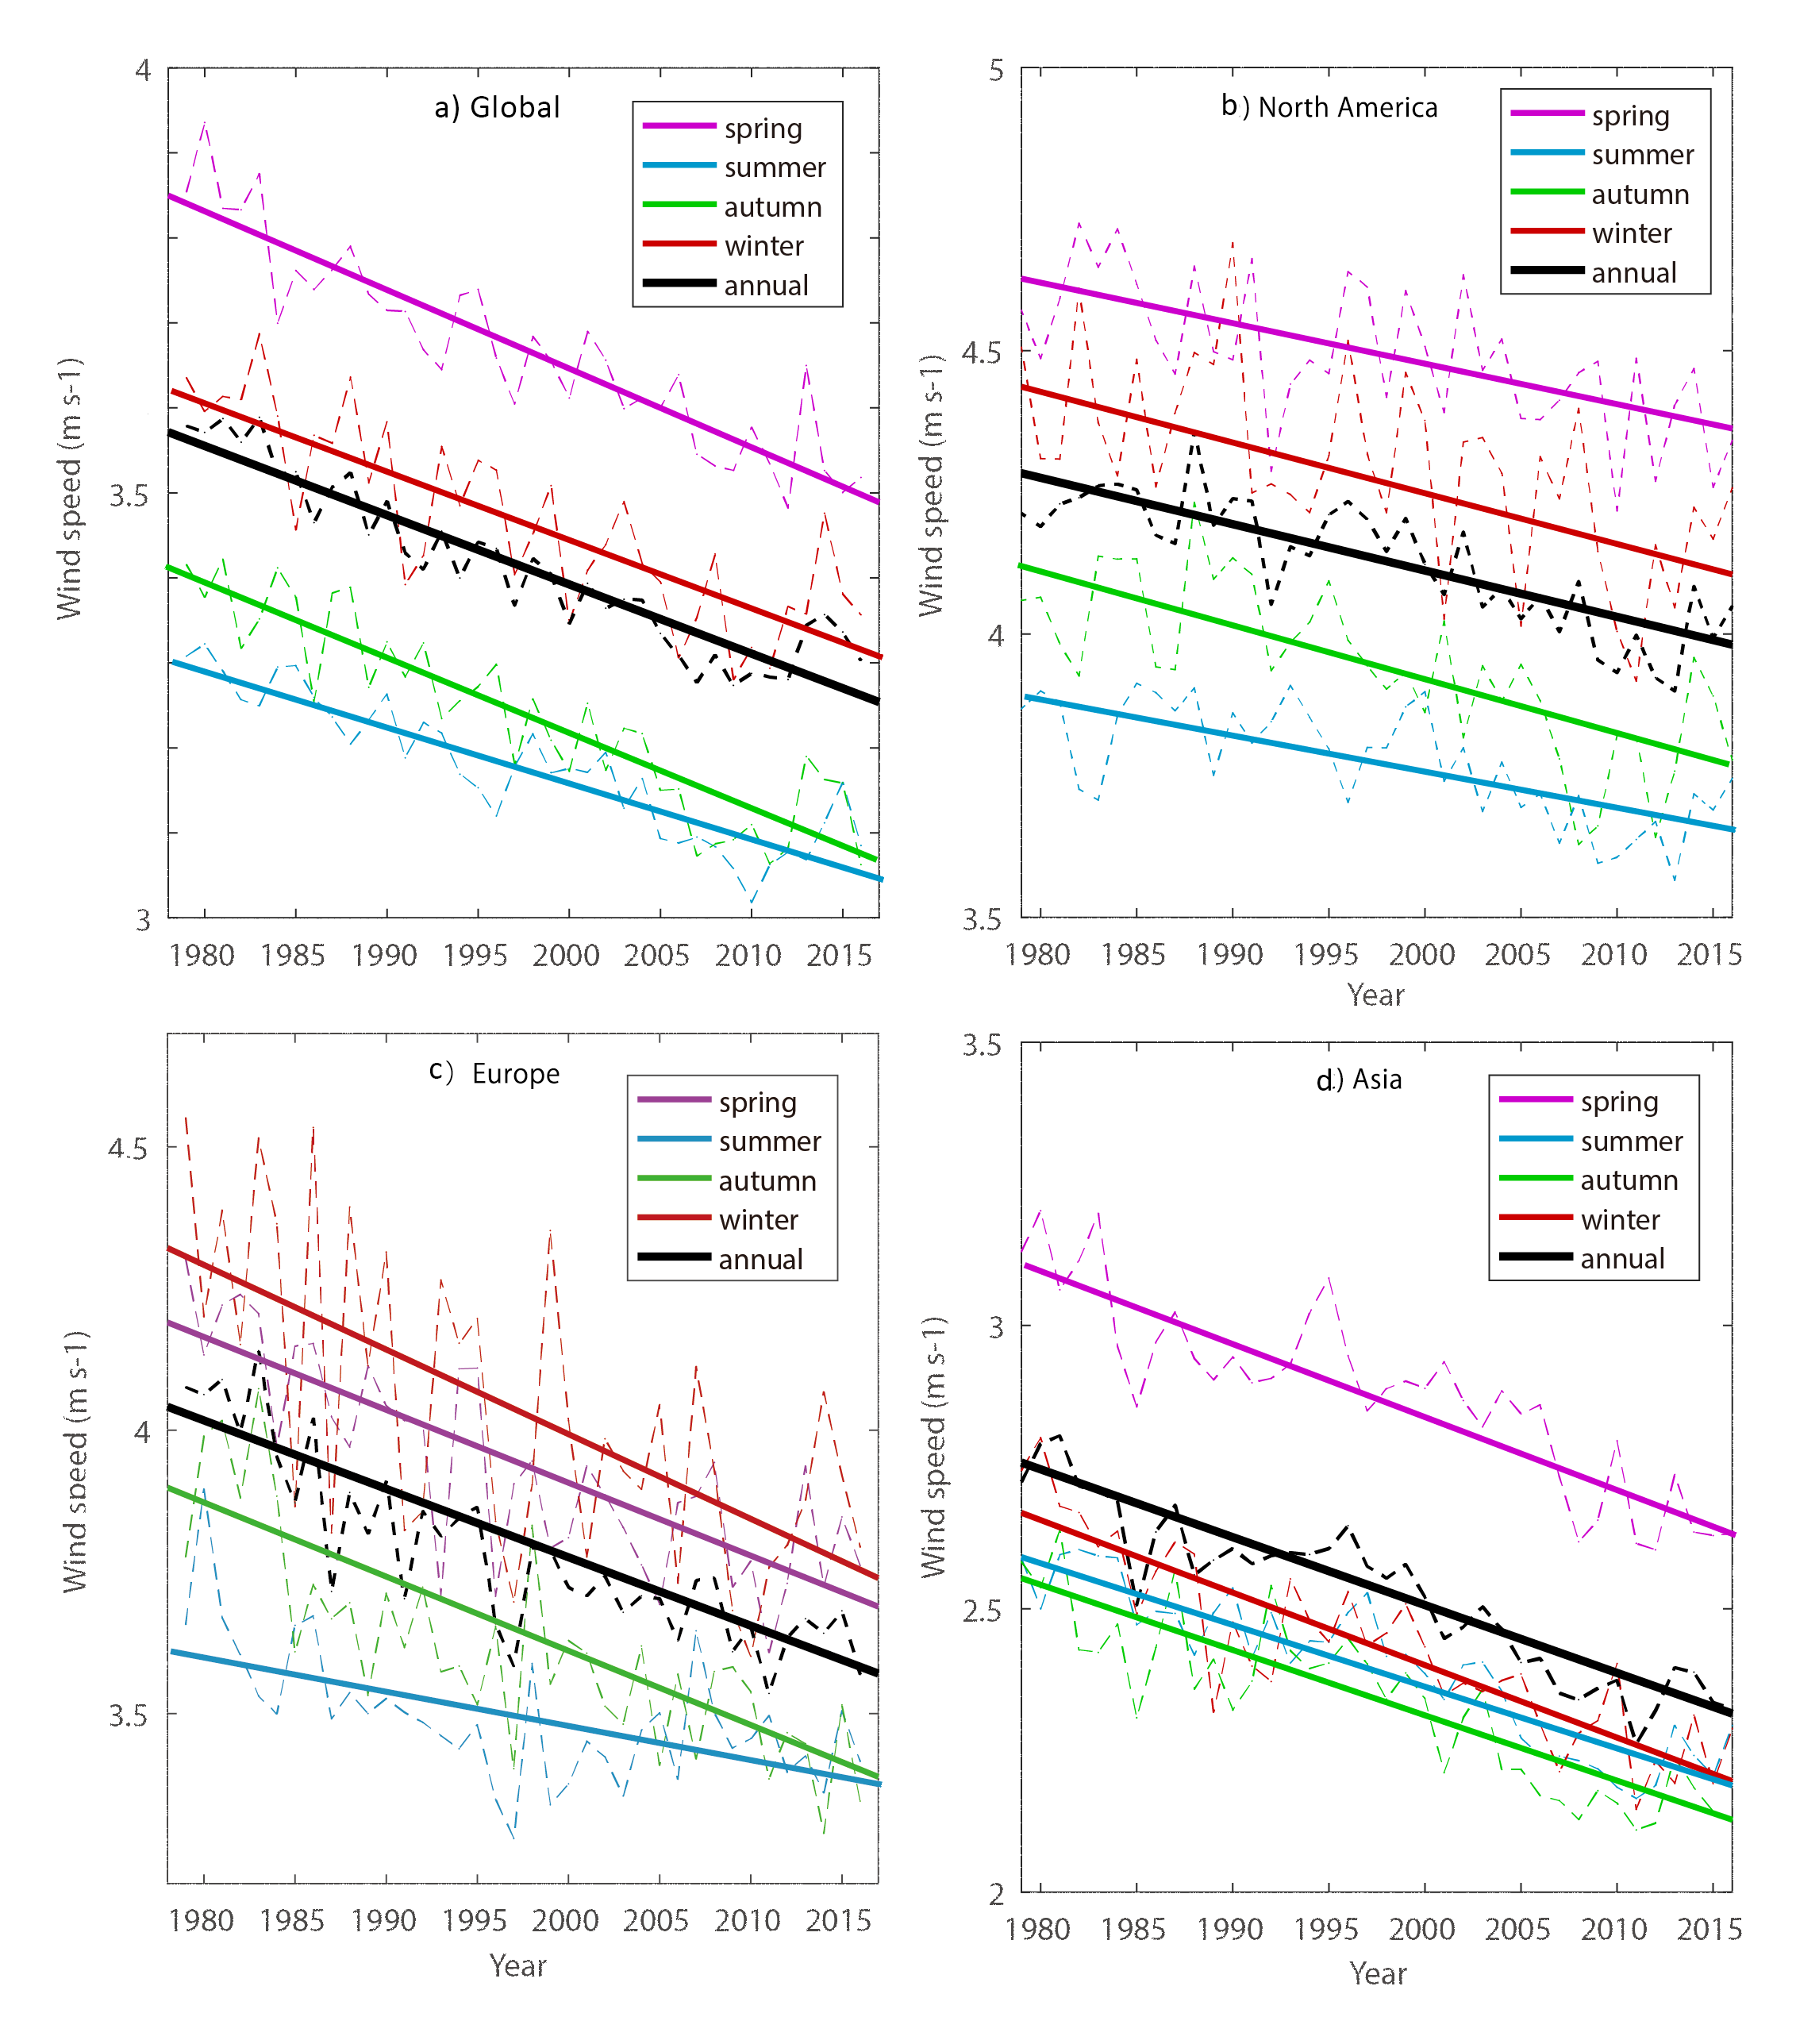
\includegraphics[width=0.9\textwidth]{各大洲中位数风速趋势}
    \bicaption{各大洲中位数风速趋势。a)全球,b)北美,c)欧洲,d)亚洲。紫色为春季,蓝色为夏季,绿色为秋季,红色为冬季,黑色为年平均。虚线为各年对应值,实线为虚线的线性趋势。}{Global and regional median wind speed trends. a)Global, b)North America, c)Europe, d)Asia. Purple color denotes spring, blue denotes summer, green denotes fall, red denotes winter, black denotes annual mean. Dash line denotes value for every year, soild line is linear trend line of dash line.}
    \label{fig:regionalmedianwindtrend}
\end{figure}

将一年划分为四个季节,分别是春季(3 - 5月)、夏季(6 - 8月)、秋季(9 - 11月)和冬季(12月至次年2月),风速在不同季节的长期线性趋势有一定差异。全球平均来看,平均风速和趋势的季节间差异明显,春季平均风速最大同时下降最快(-0.089 $m ~ s^{-1}$每十年),夏季平均风速最小同时下降最慢(-0.065 $m ~ s^{-1}$每十年)(图 \ref{fig:regionalmedianwindtrend} a))。在北美洲,平均风速春季最大而夏季最小,分别为4.5 $m ~ s^{-1}$和3.75 $m ~ s^{-1}$。风速在四季均出现了下降,秋季下降最快,达到-0.094 $m ~ s^{-1}$每十年(季节平均风速长期趋势的空间中位数,本段以下所提到的趋势均是此种方法计算),而夏季最慢,为-0.073 $m ~ s^{-1}$每十年。归一化风速趋势上(即趋势/气候态),秋季为-2.2\%每十年,为四季中最快,与之相对,春季为-1.7\%每十年,为四季中最慢。空间分布上四季差异不明显(图 \ref{fig:regionalmedianwindtrend} b),图 \ref{fig:NAwindtrend})。在欧洲,平均风速冬季最大(4.07 $m ~ s^{-1}$)而夏季最小(3.5 $m ~ s^{-1}$)。风速同样在四季都呈下降趋势,其中秋季下降最快,为-0.12 $m ~ s^{-1}$每十年,夏季趋势最平缓,为-0.072 $m ~ s^{-1}$每十年,归一化趋势四季分别为-2.8\%、-2.1\%、-3.3\%和-2.5\%每十年。空间分布上,东欧地区秋冬两季下降明显快于春夏,奥地利和斯洛文尼亚风速增加在春、秋、冬季快于夏季,英国和北爱尔兰风速下降在秋季达到最大值而夏季最小(图 \ref{fig:regionalmedianwindtrend} c),图 \ref{fig:EUwindtrend})。在亚洲,春季平均风速显著大于另外三个季节,达到2.8 $m ~ s^{-1}$,夏秋冬平均在2.4 $m ~ s^{-1}$左右。四季风速趋势都为负值,其中春季下降最快,达到-0.103 $m ~ s^{-1}$每十年,冬季最慢,为-0.057 $m ~ s^{-1}$每十年,归一化风速趋势排序与此相同,即春季最快(-3.9\% 每十年)而冬季最慢(-2.7\% 每十年)。空间分布上,中国东北地区春季风速下降明显快于其他季节,中国中部地区的风速增加在夏季最为剧烈(图 \ref{fig:regionalmedianwindtrend} d), 图 \ref{fig:ASwindtrend})。


\begin{figure}[!htbp]
    \centering
    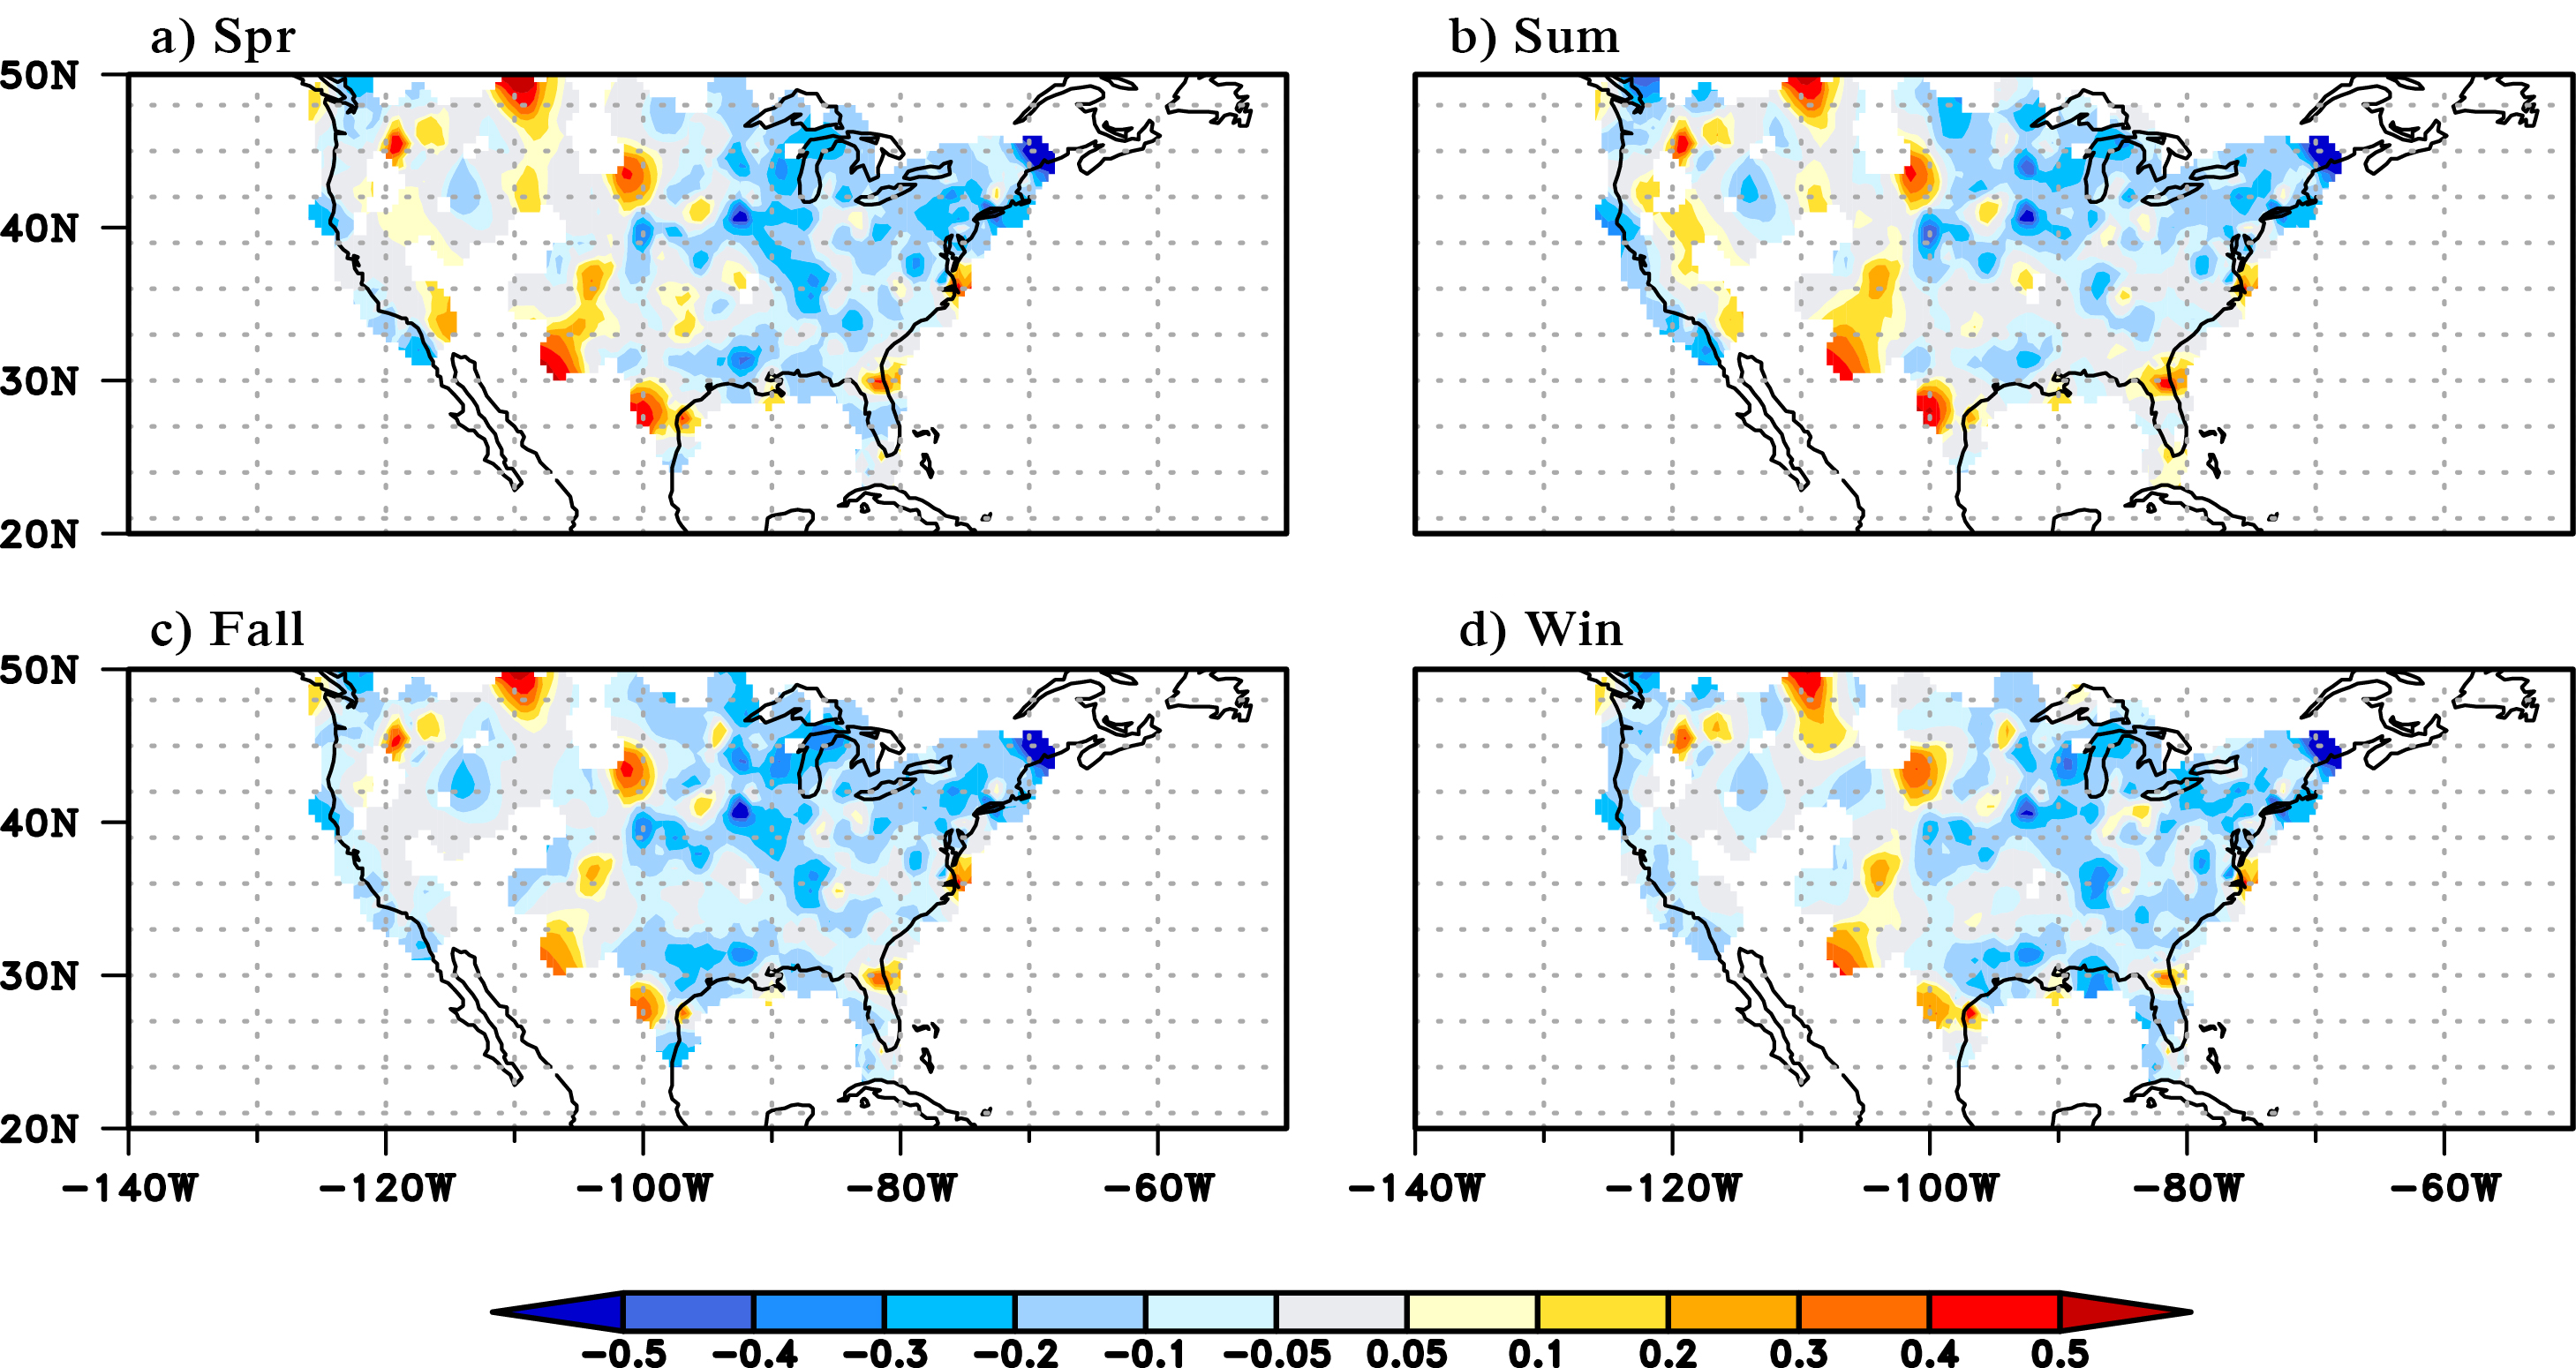
\includegraphics[width=0.85\textwidth]{北美洲四季风速长期趋势}
    \bicaption{北美四季风速长期趋势 ($m ~ s^{-1}$每十年)。a)春季(3-5月),b)夏季(6-8),c)秋季(9-11月),d)冬季(12月-次年2月)}{Long-term seasonal wind speed trends over North America (in $m ~ s^{-1} ~ decade^{-1}$). a) Spring (March to May), b) Summer (June to August), c) Fall (September to November), d) Winter (December to next February).}
    \label{fig:NAwindtrend}
\end{figure}

\begin{figure}[!htbp]
    \centering
    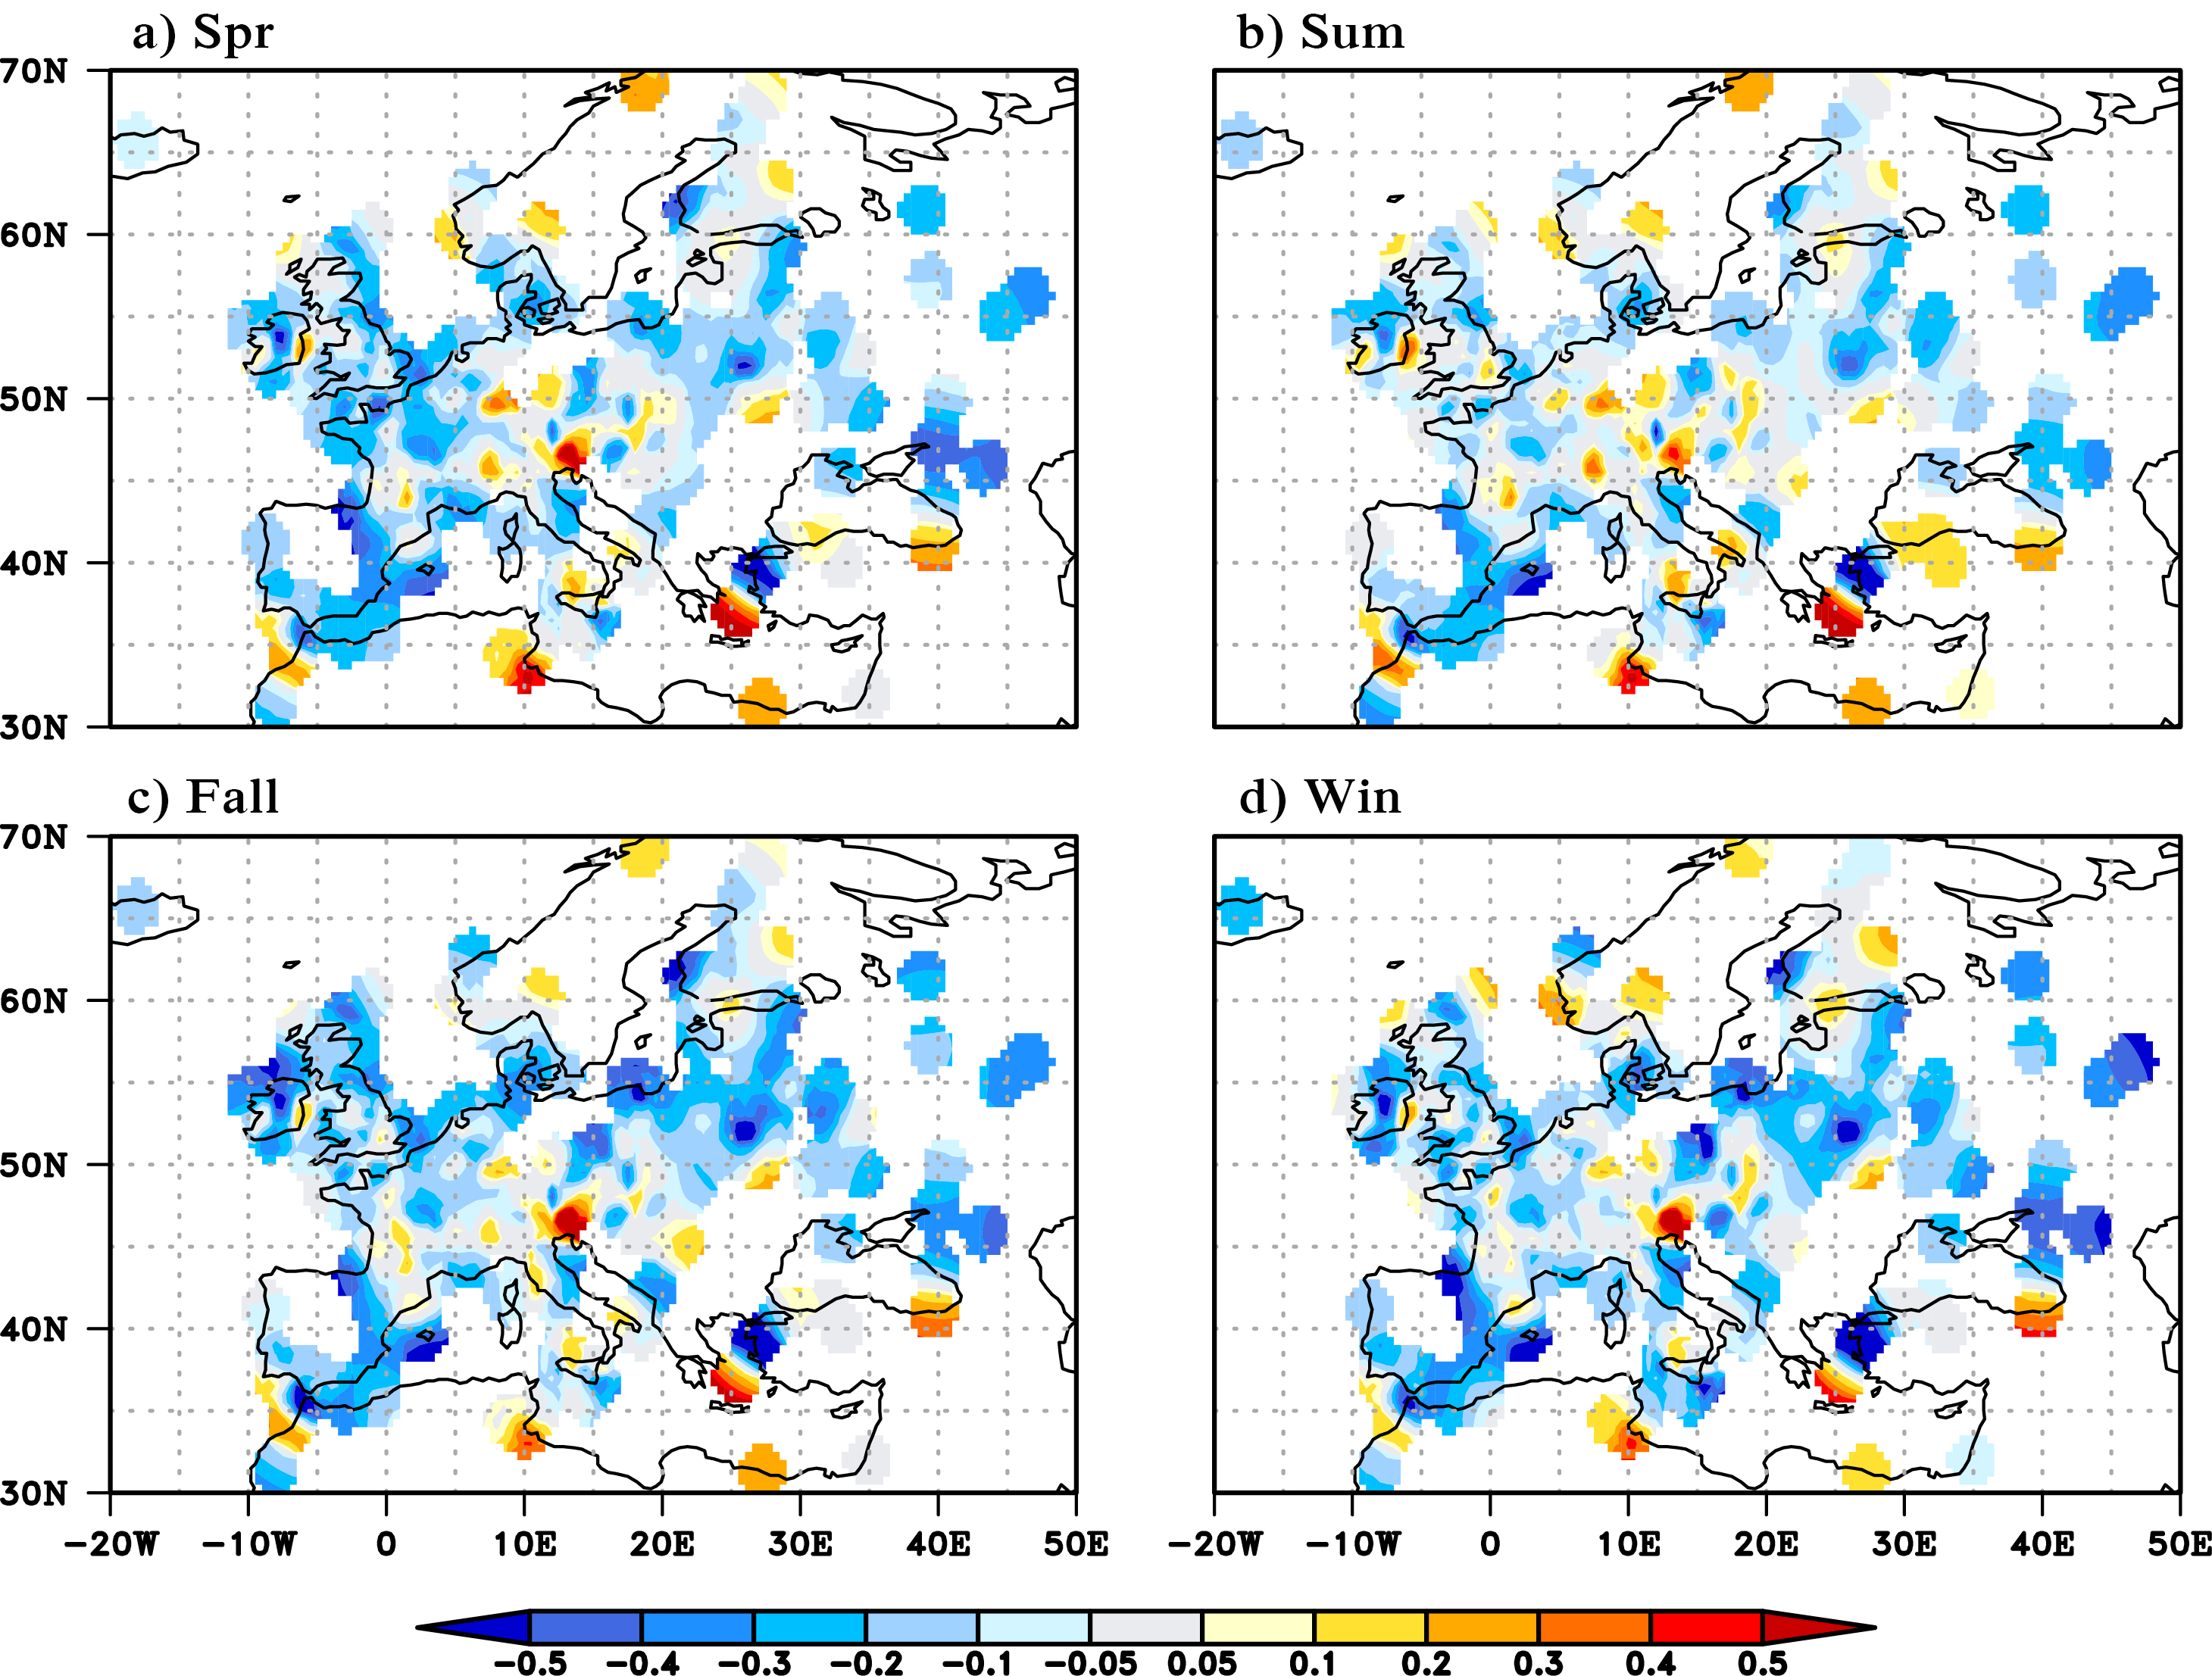
\includegraphics[width=0.85\textwidth]{欧洲四季风速长期趋势}
    \bicaption{欧洲四季风速长期趋势。与图 \ref{fig:NAwindtrend} 类似。}{Same as Figure \ref{fig:NAwindtrend}, but for Europe.}
    \label{fig:EUwindtrend}
\end{figure}

\begin{figure}[!htbp]
    \centering
    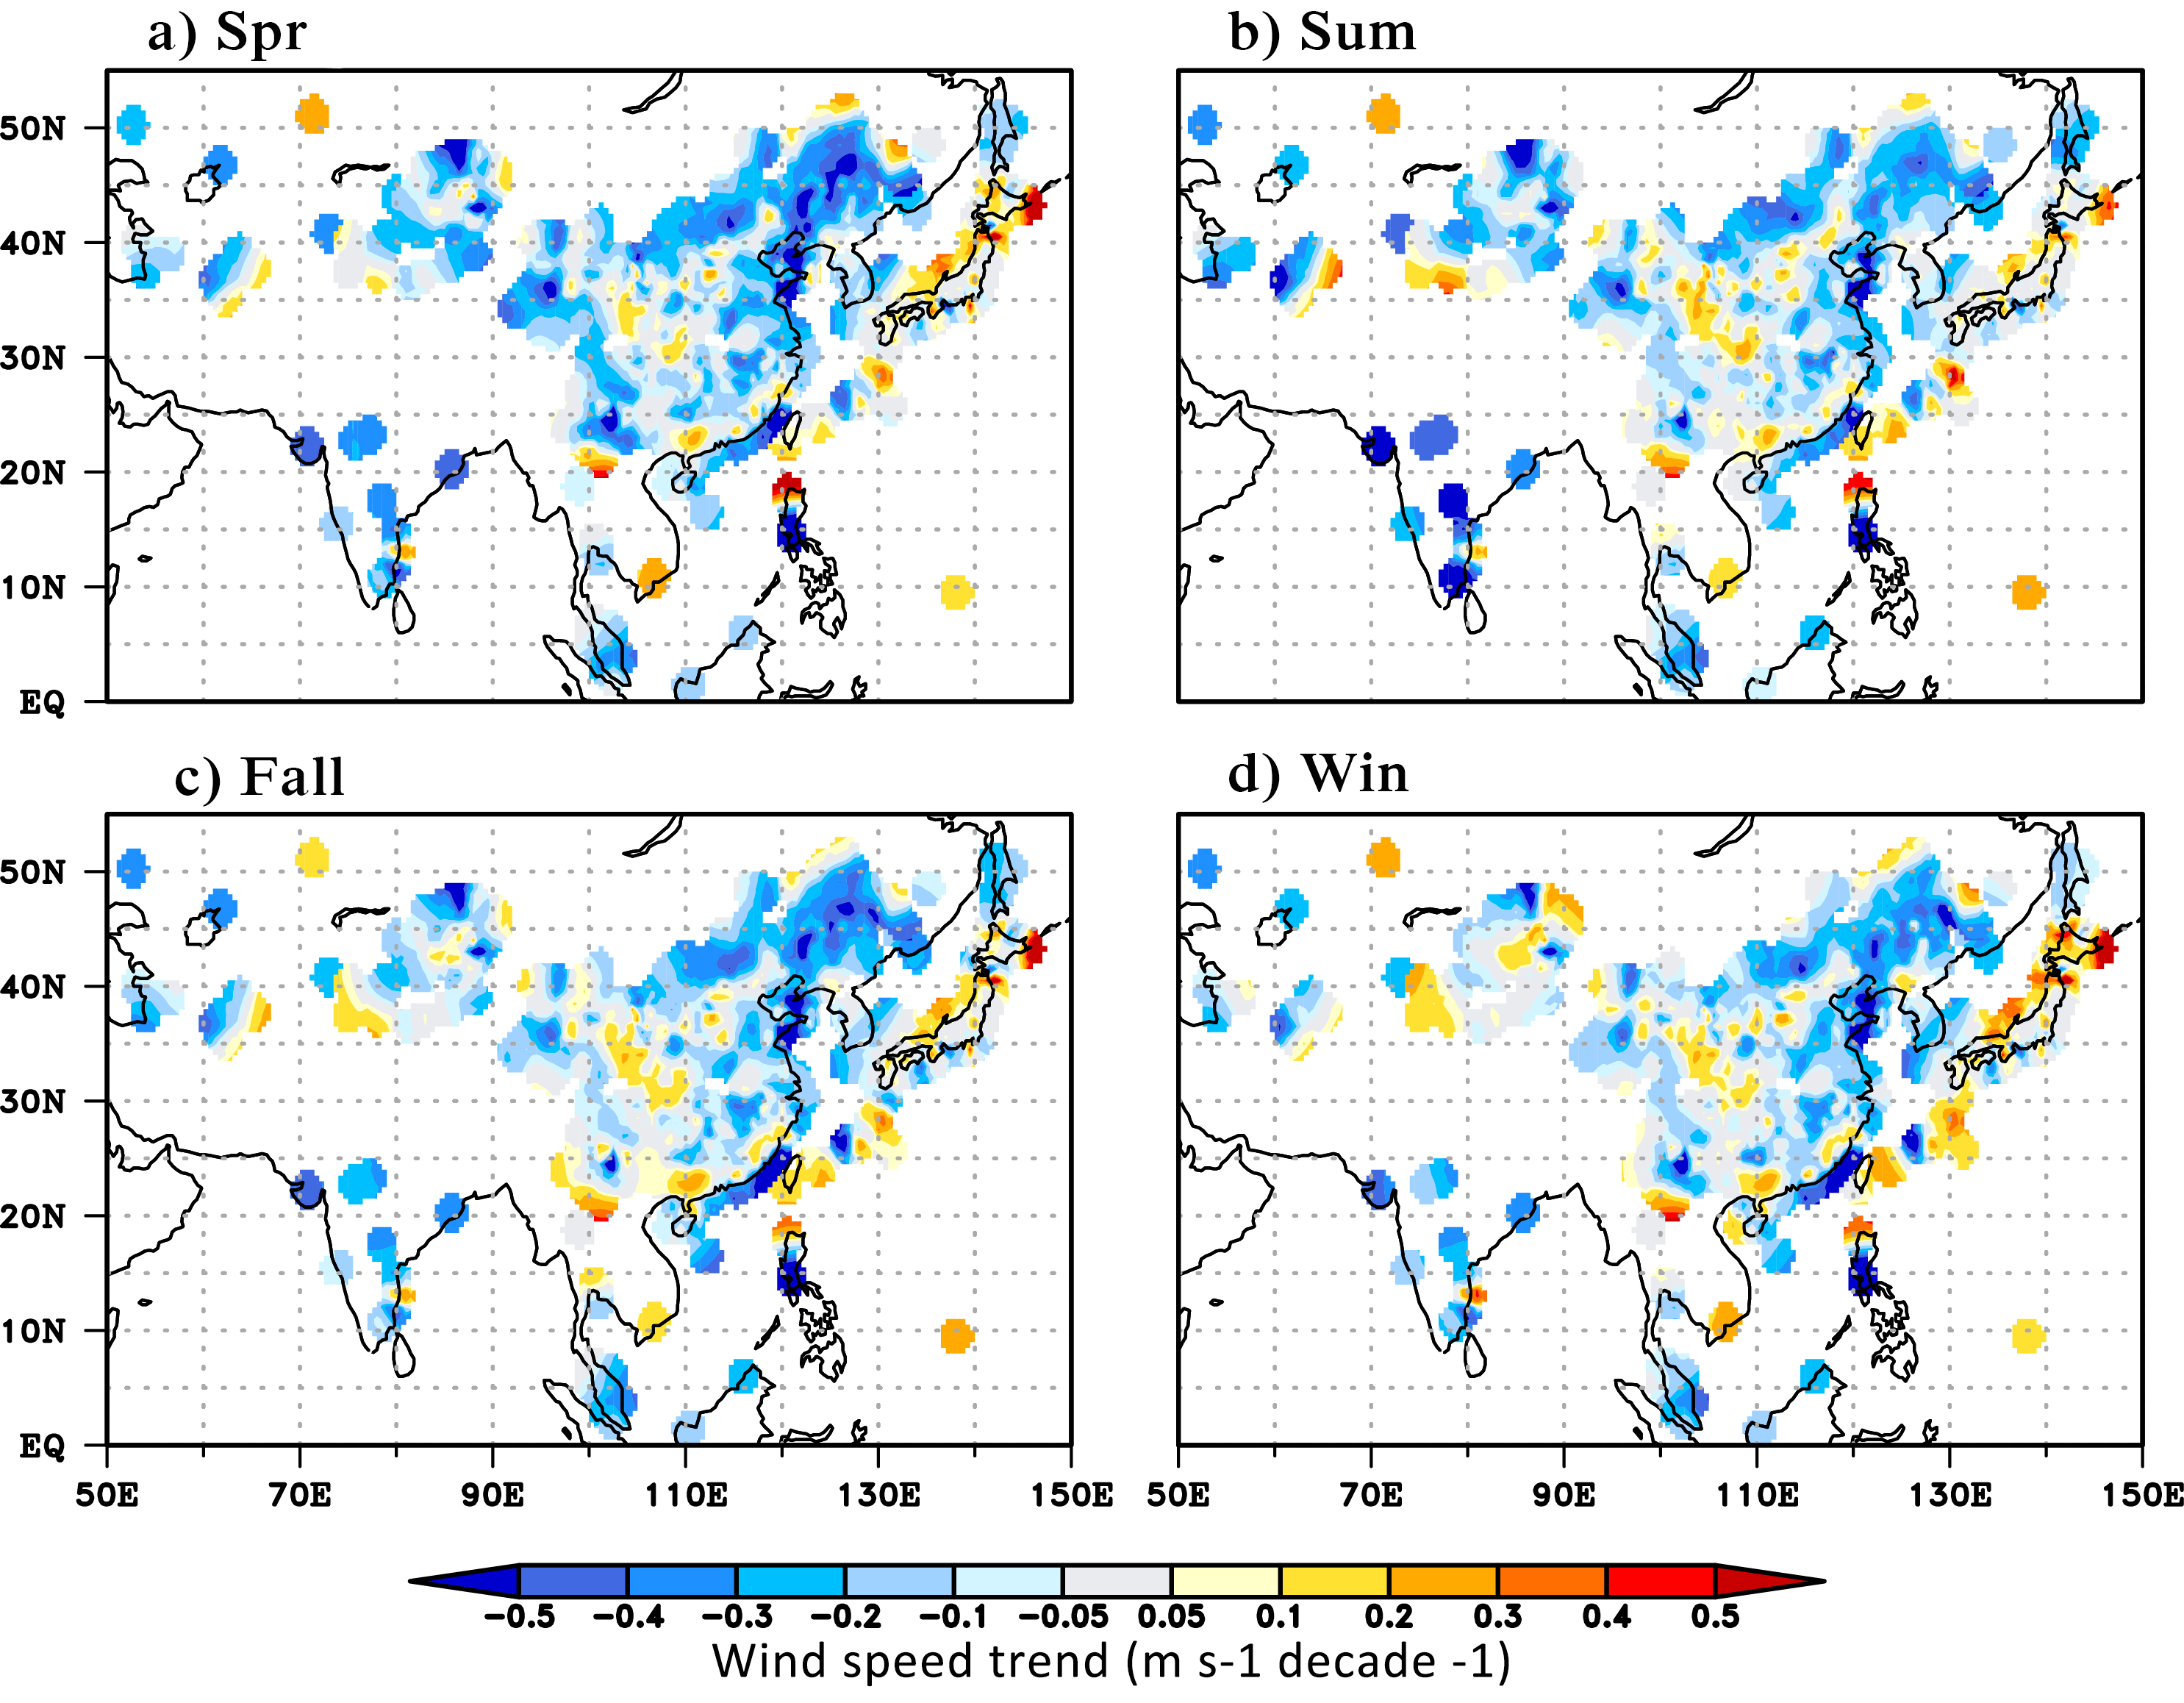
\includegraphics[width=0.85\textwidth]{亚洲四季风速长期趋势}
    \bicaption{亚洲四季风速长期趋势。与图 \ref{fig:NAwindtrend} 类似。}{Same as Figure \ref{fig:NAwindtrend}, but for Asia.}
    \label{fig:ASwindtrend}
\end{figure}

\subsection{不同海拔站点风速长期线性趋势}

根据\href{https://community.wmo.int/activity-areas/imop/cimo-guide/cimo-guide-preliminary-2018-edition}{国际气象组织(WMO)观测规范},地面观测风速在地面以上10 m高度,现有的大部分常规地面风速观测都遵照此规范进行。然而,由于地形的起伏,实际观测的海拔高度有较大差别,最高海拔可以达到5000 m左右,而最低在海平面以下。对不同海拔的地表风速长期趋势进行分析,发现具有一定的倾向性。在北美洲,总共有214个站点,其中海拔在500 m 以上的约为20\%,1000 m以上的约10\%。随着海拔的增加,风速趋向于上升(p < 0.01),倾向率为0.018\% 每十年(图 \ref{fig:regionalwindvselevation} a))。在欧洲,绝大多数站点海拔在500 m以下,在总共224个站点中仅有9个海拔超过500 m。与北美洲类似,欧洲风速趋势随海拔增加而趋向于正(p < 0.05),倾向率0.0256\% 每十年(图 \ref{fig:regionalwindvselevation} b))。在亚洲,由于青藏高原等大地形的存在,观测站海拔分布较为分散,在总共531个站点中,有约20\% 分布在1000 m以上,有7\% 在2000 m以上。然而,此区域风速趋势与海拔没有明显的相关性(图 \ref{fig:regionalwindvselevation} c))。

\begin{figure}[!htbp]
    \centering
    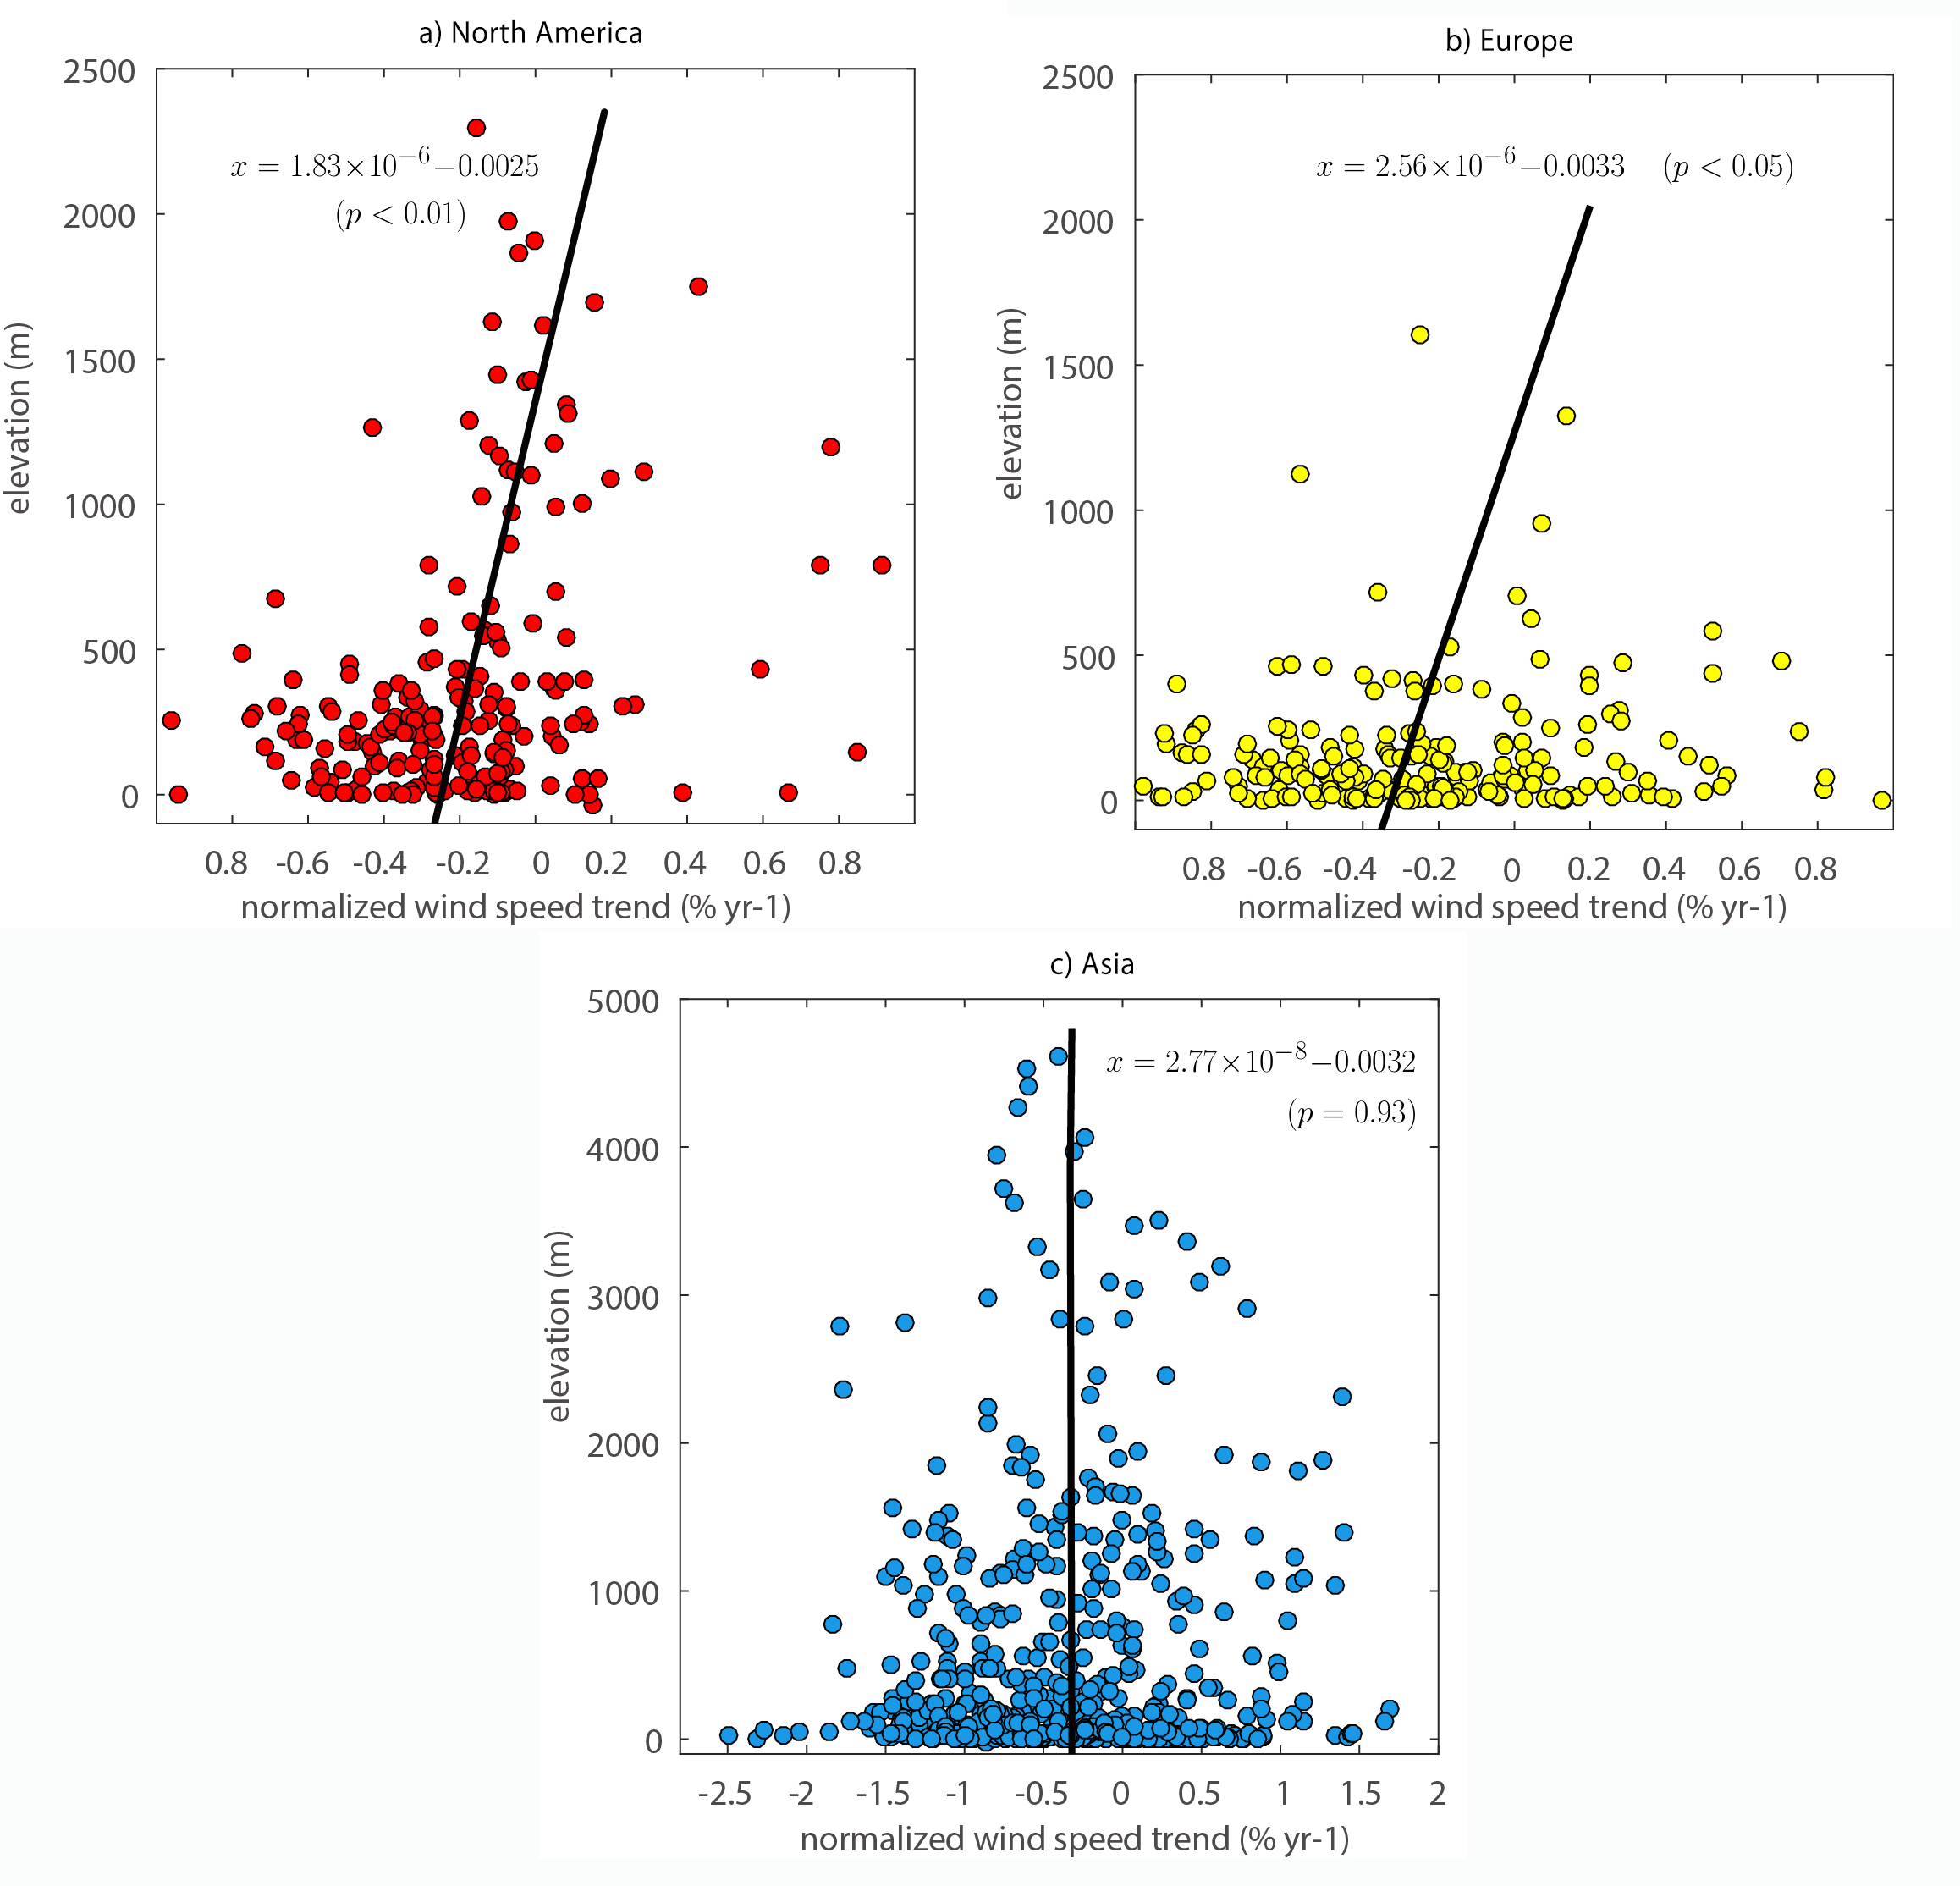
\includegraphics[width=0.9\textwidth]{各大洲归一化风速趋势与海拔的关系}
    \bicaption{各大洲归一化风速趋势与海拔的关系。a)北美洲,b)欧洲,c)亚洲。}{Normalized wind speed trends versus elevation in every continent. a)North America, b)Europe, c)Asia.}
    \label{fig:regionalwindvselevation}
\end{figure}

\section{北半球陆地地表风速趋势的年代际变化}

\begin{figure}[!b]
    \centering
    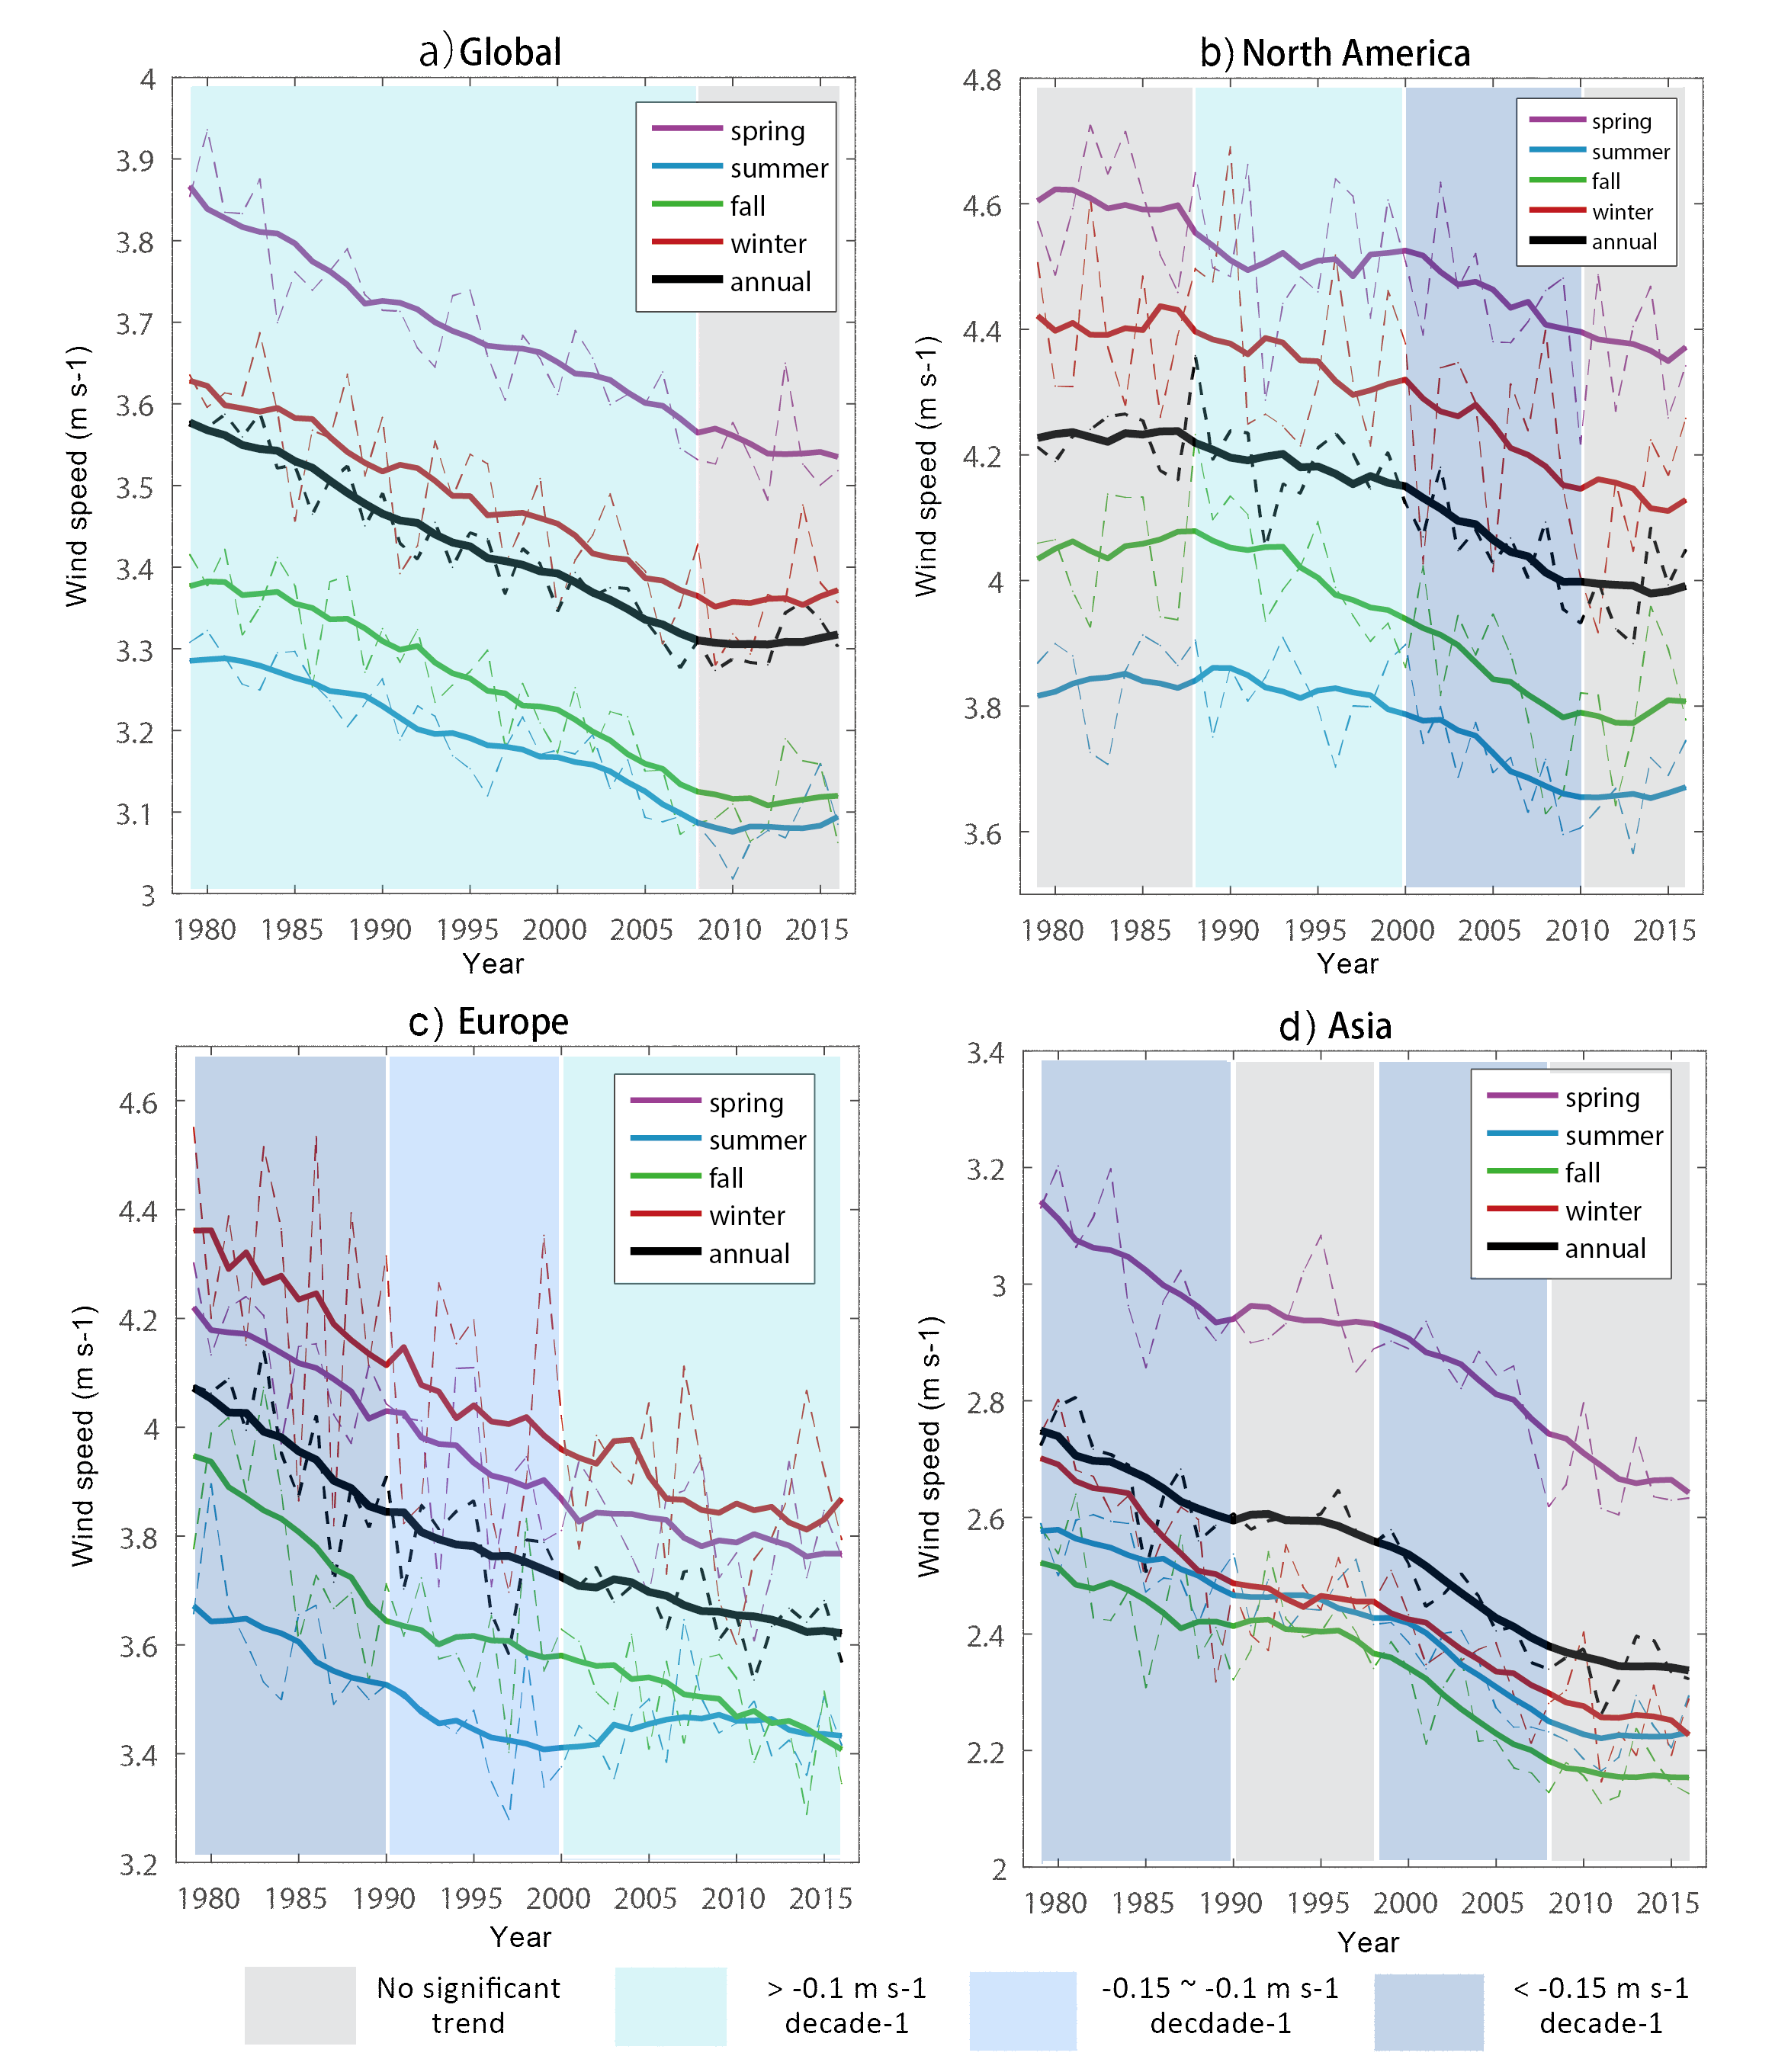
\includegraphics[width=0.9\textwidth]{各大洲中位数风速年代际演变}
    \bicaption{各大洲中位数风速年代际演变。a)全球,b)北美,c)欧洲,d)亚洲。紫色为春季,蓝色为夏季,绿色为秋季,红色为冬季,黑色为年平均。虚线为各年对应值,实线为虚线9点平滑的结果。底色为灰色、浅蓝、蓝色、深蓝的时段分别代表年平均风速无明显趋势、慢速下降、中速下降和快速下降。}{Decadal evolution of global and regional median wind speeds.  a)Global, b)North America, c)Europe, d)Asia. Purple color denotes spring, blue denotes summer, green denotes fall, red denotes winter, black denotes annual mean. Dash line denotes value for every year, soild line is 9-point moving mean of dash line. Periods with grey, light blue, blue, dark blue represent time when annual mean wind speeds have no trend, go down slowly, go down with medium speed, go down sharply, respectively.}
    \label{fig:regionalmedianwinddecadalchange}
\end{figure}

全球以及各大洲陆地地表风速趋势在不同年代际表现出了不同特征。全球平均来看,年平均风速趋势在2007年前后发生了一次显著变化(滑动t检验去趋势序列 p < 0.01,本段以下所提到年代际突变均采用此种方式计算得到),1979-2007年的趋势为-0.092 $m ~ s^{-1}$每十年,2007-2016年无明显趋势。这种年代际变化由夏、秋、冬季贡献,春季几乎没有体现出2007年后趋势减弱的现象(图 \ref{fig:regionalmedianwinddecadalchange} a))。在北美洲,年平均风速大致经历了1987年前平稳时期(无明显趋势),1987-2000缓慢下降时期(-0.059 $m ~ s^{-1}$每十年),2000-2010快速下降时期(-0.160 $m ~ s^{-1}$每十年)和2010年后平稳时期(无明显趋势)。1987年前风速较为平稳和2000-2010年快速下降在四季均有体现,而1981-2000四季表现差异较大,2010年后夏、秋季风速出现上升,春、冬季风速继续下降(图 \ref{fig:regionalmedianwinddecadalchange} b))。在欧洲,年平均风速经历了1990年前快速下降(-0.254 $m ~ s^{-1}$每十年),1990-2000中速下降(-0.131 $m ~ s^{-1}$每十年)和2000年后缓慢下降(-0.072 $m ~ s^{-1}$每十年)三个时期。冬季风速突变点大致与年平均风速相同,而春季和秋季经历了两个时期,即快速下降和缓慢下降时期,突变点分别在2000和1993年。夏季最为特殊,2000年前风速下降,其后风速逐渐上升(图 \ref{fig:regionalmedianwinddecadalchange} c))。在亚洲,风速在1990年前快速下降(-0.190 $m ~ s^{-1}$每十年),1990-1997年趋于平稳 (无明显趋势),1997-2007再次快速下降(-0.206 $m ~ s^{-1}$每十年),2007年后再次趋于平稳(无明显趋势)。四季风速均与年平均风速年代际变化较为吻合(图 \ref{fig:regionalmedianwinddecadalchange} d))。

\section{北半球陆地地表风速长期变化的不确定性分析}

如第\ref{chap:intro}章所述,观测风速可能由于仪器更换、观测环境变化等,不能反映出真实的变化,尽管本章分析使用的风速序列经过了严格质量控制,依然不能完全排除上述人为因素的影响。为此,使用NCEP/NCAR、NCEP-DOE、ERA-Interim、JRA-55和MERRA-2等5套再分析资料再次计算陆地地表风速的长期变化,并与观测进行对比。值得一提的是,除JRA-55外,其他4套再分析资料均没有同化陆地地表风速观测。以下分析基于5套再分析资料10 m U、V风场计算的年平均风速差值到观测点的结果。

\subsection{风速长期线性趋势的不确定性}

\begin{figure}[!t]
    \centering
    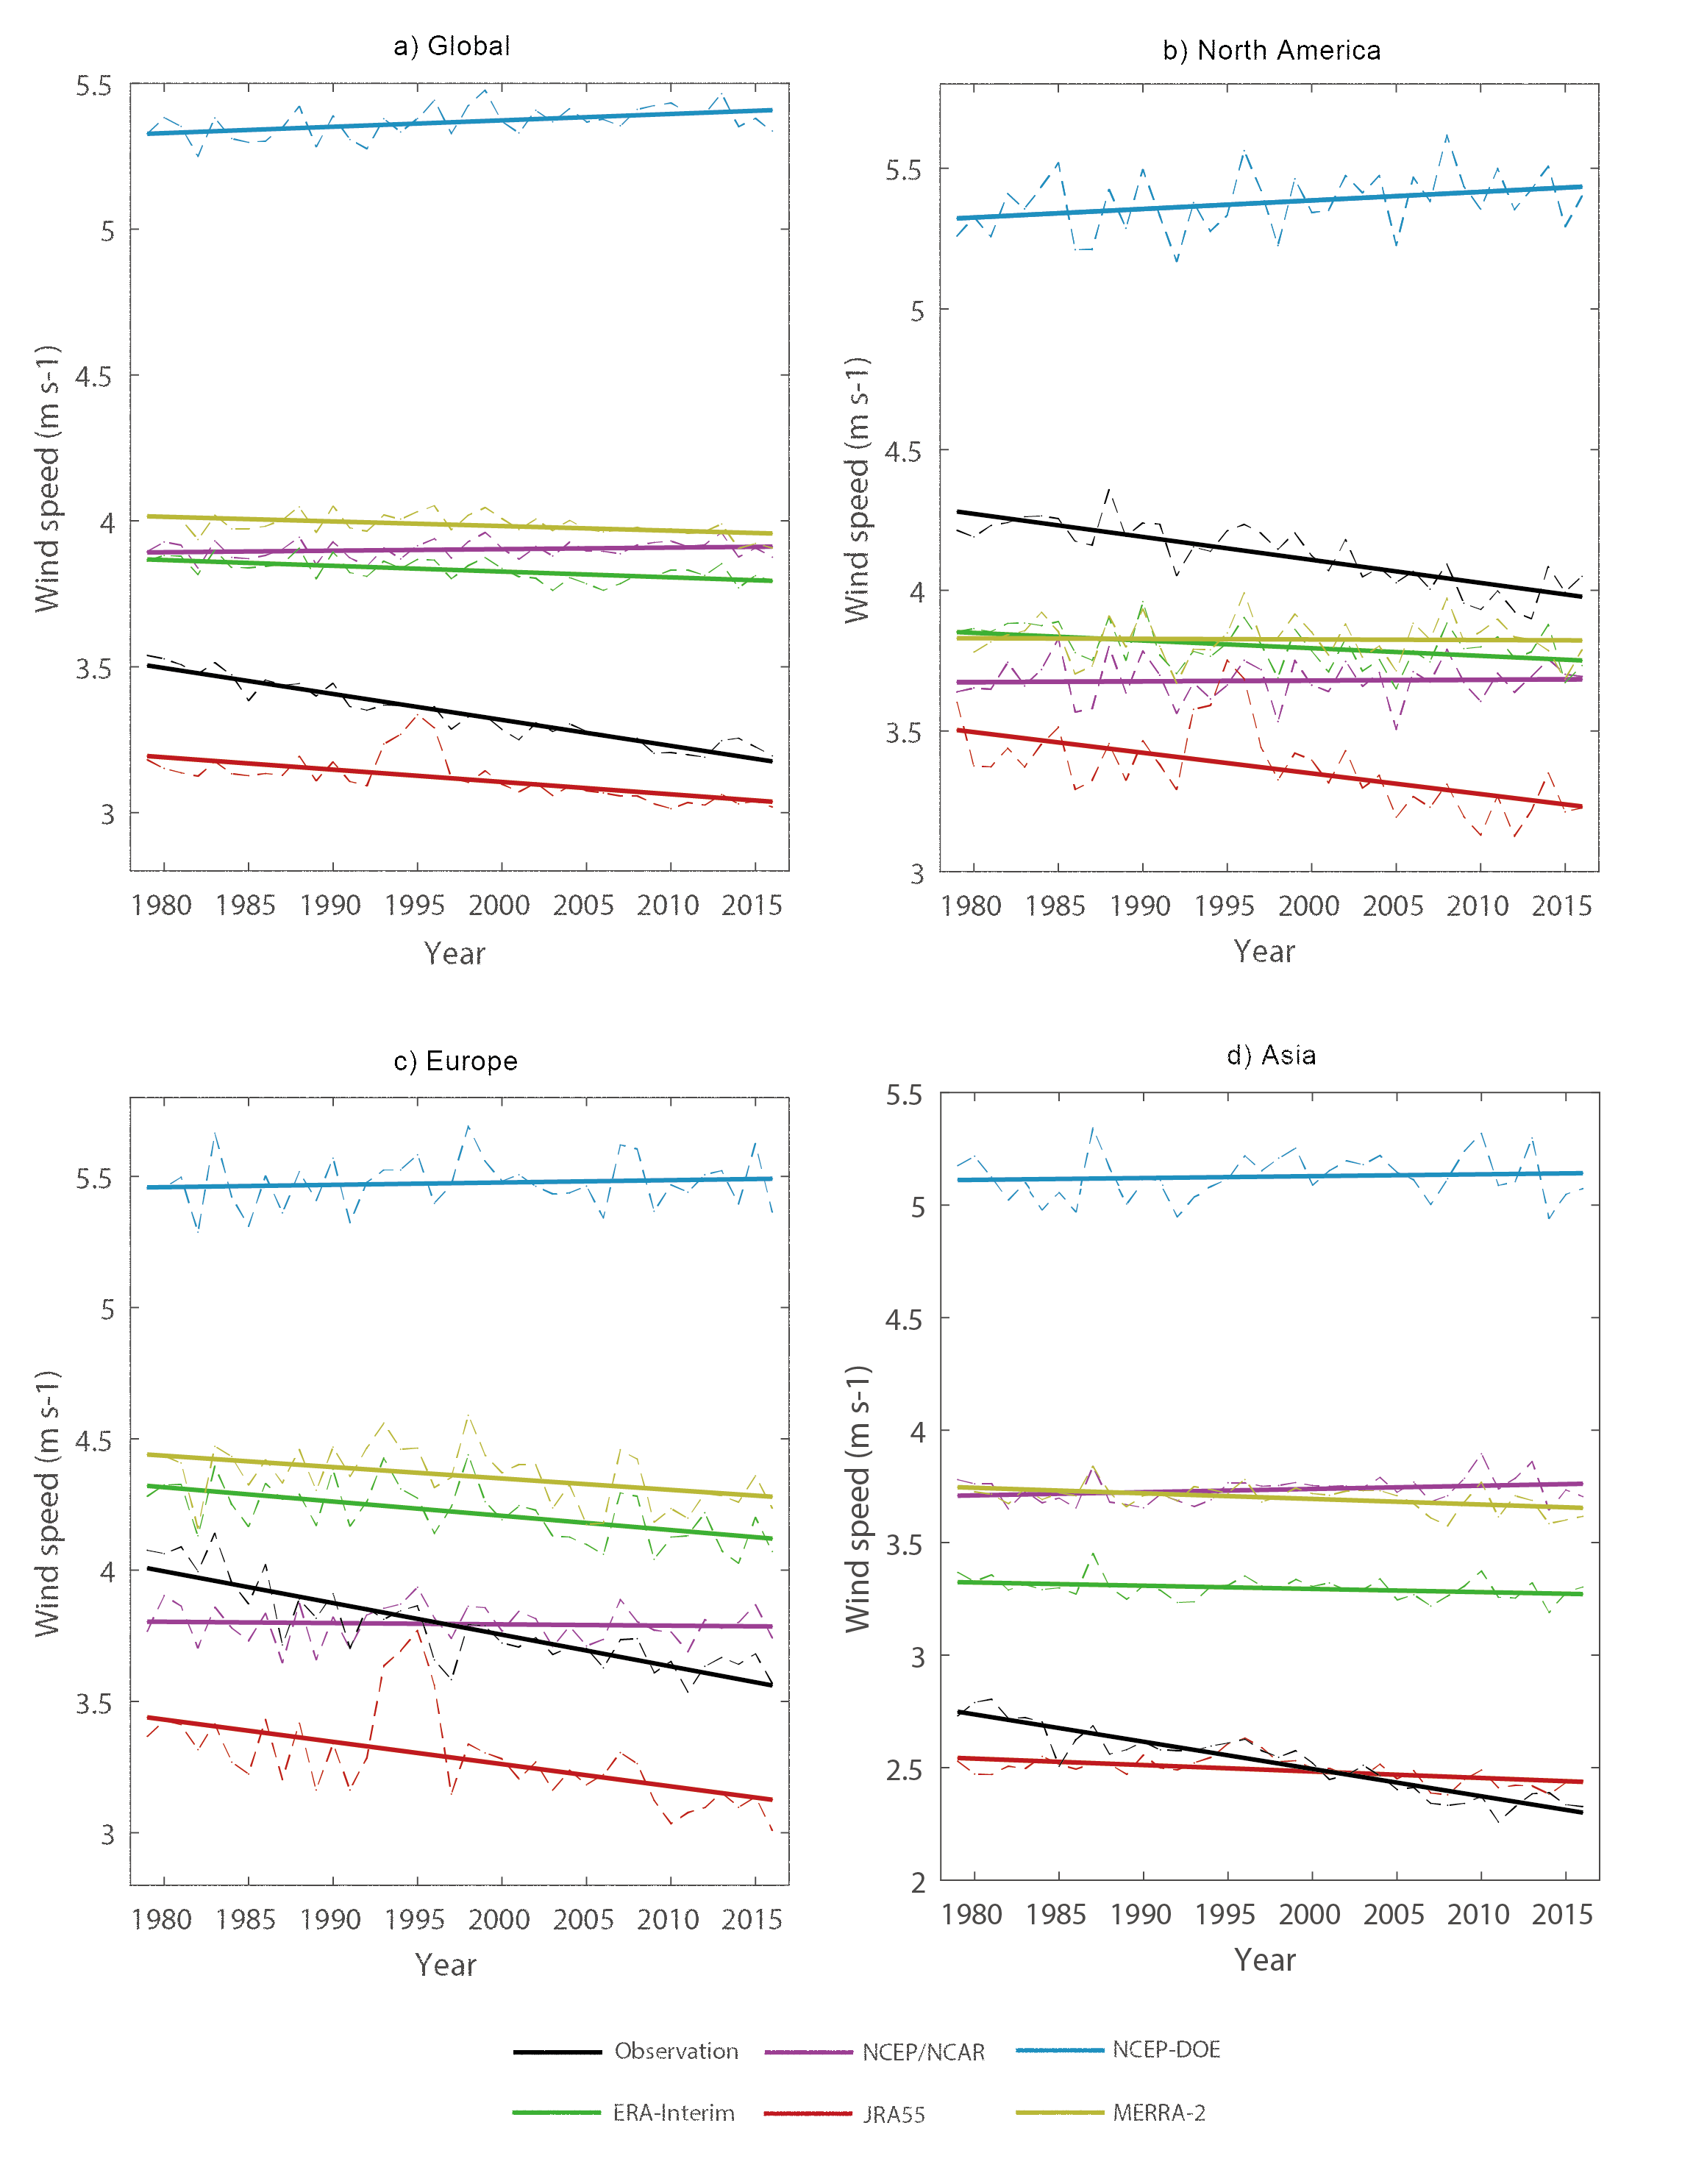
\includegraphics[width=0.9\textwidth]{风速趋势不确定性}
    \bicaption{观测及再分析资料风速长期线性趋势。a)全球,b)北美洲,c)欧洲,d)亚洲。虚线为年均值,实线为虚线的线性趋势。}{Wind speed trends in observation and reanalysis data. a)Global, b)North America, c) Europe, d)Asia. Dash line is annual mean value, solid line is linear trend line of dash line.}
    \label{fig:uncertaintywindtrend}
\end{figure}

全球平均风速上,NCEP-DOE风速明显偏大,与其他4套再分析资料及观测相差大于1 $m ~ s^{-1}$,NCEP/NCAR、ERA-Interim和MERRA-2非常接近,且都略大于观测(差别约0.5 $m ~ s^{-1}$),而JRA-55略小于观测(差别约0.3 $m ~ s^{-1}$)。风速长期趋势上,NCEP-DOE和ERA-Interim呈微弱上升趋势,分别为0.022和0.020 $m ~ s^{-1}$每十年;NCEP/NCAR无明显趋势;MERRA-2、JRA-55都呈现出下降趋势,分别为-0.016和-0.042 $m ~ s^{-1}$每十年,然而它们的下降速度都不及观测(-0.081 $m ~ s^{-1}$每十年)(图 \ref{fig:uncertaintywindtrend} a))。在北美洲,平均风速NCEP-DOE最大,其他4套再分析资料均小于观测,JRA-55最小。风速长期趋势上,NCEP-DOE风速以0.03 $m ~ s^{-1}$每十年的趋势上升,MERRA-2和NCEP/NCAR基本不变,ERA-Interim和JRA55分别以-0.027和-0.073 $m ~ s^{-1}$每十年的趋势下降,观测风速趋势为-0.075 $m ~ s^{-1}$每十年(图 \ref{fig:uncertaintywindtrend} b))。在欧洲,平均风速除NCEP-DOE偏大外,MERRA-2和ERA-Interim略大于观测,JRA-55略小于观测,NCEP/NCAR与观测接近。风速趋势NCEP/NCAR与NCEP-DOE无明显趋势,其余3套再分析资料均呈下降趋势(ERA-Inteirm:-0.054 $m ~ s^{-1}$每十年,JRA-55:-0.085 $m ~ s^{-1}$每十年,MERRA-2:-0.043 $m ~ s^{-1}$每十年),观测风速趋势为-0.105 $m ~ s^{-1}$每十年(图 \ref{fig:uncertaintywindtrend} c))。在亚洲,平均风速除JRA-55与观测接近外其他均大于观测,NCEP-DOE差别最为显著(> 2 $m ~ s^{-1}$)。风速趋势ERA-Interim、JRA-55、MERAA-2和观测均为负值,分别为-0.014、-0.029、-0.025和-0.075 $m ~ s^{-1}$每十年,而NCEP/NCAR和NCEP-DOE无明显趋势(图 \ref{fig:uncertaintywindtrend} d))。


\subsection{风速趋势年代际变化的不确定性}

\begin{figure}[!b]
    \centering
    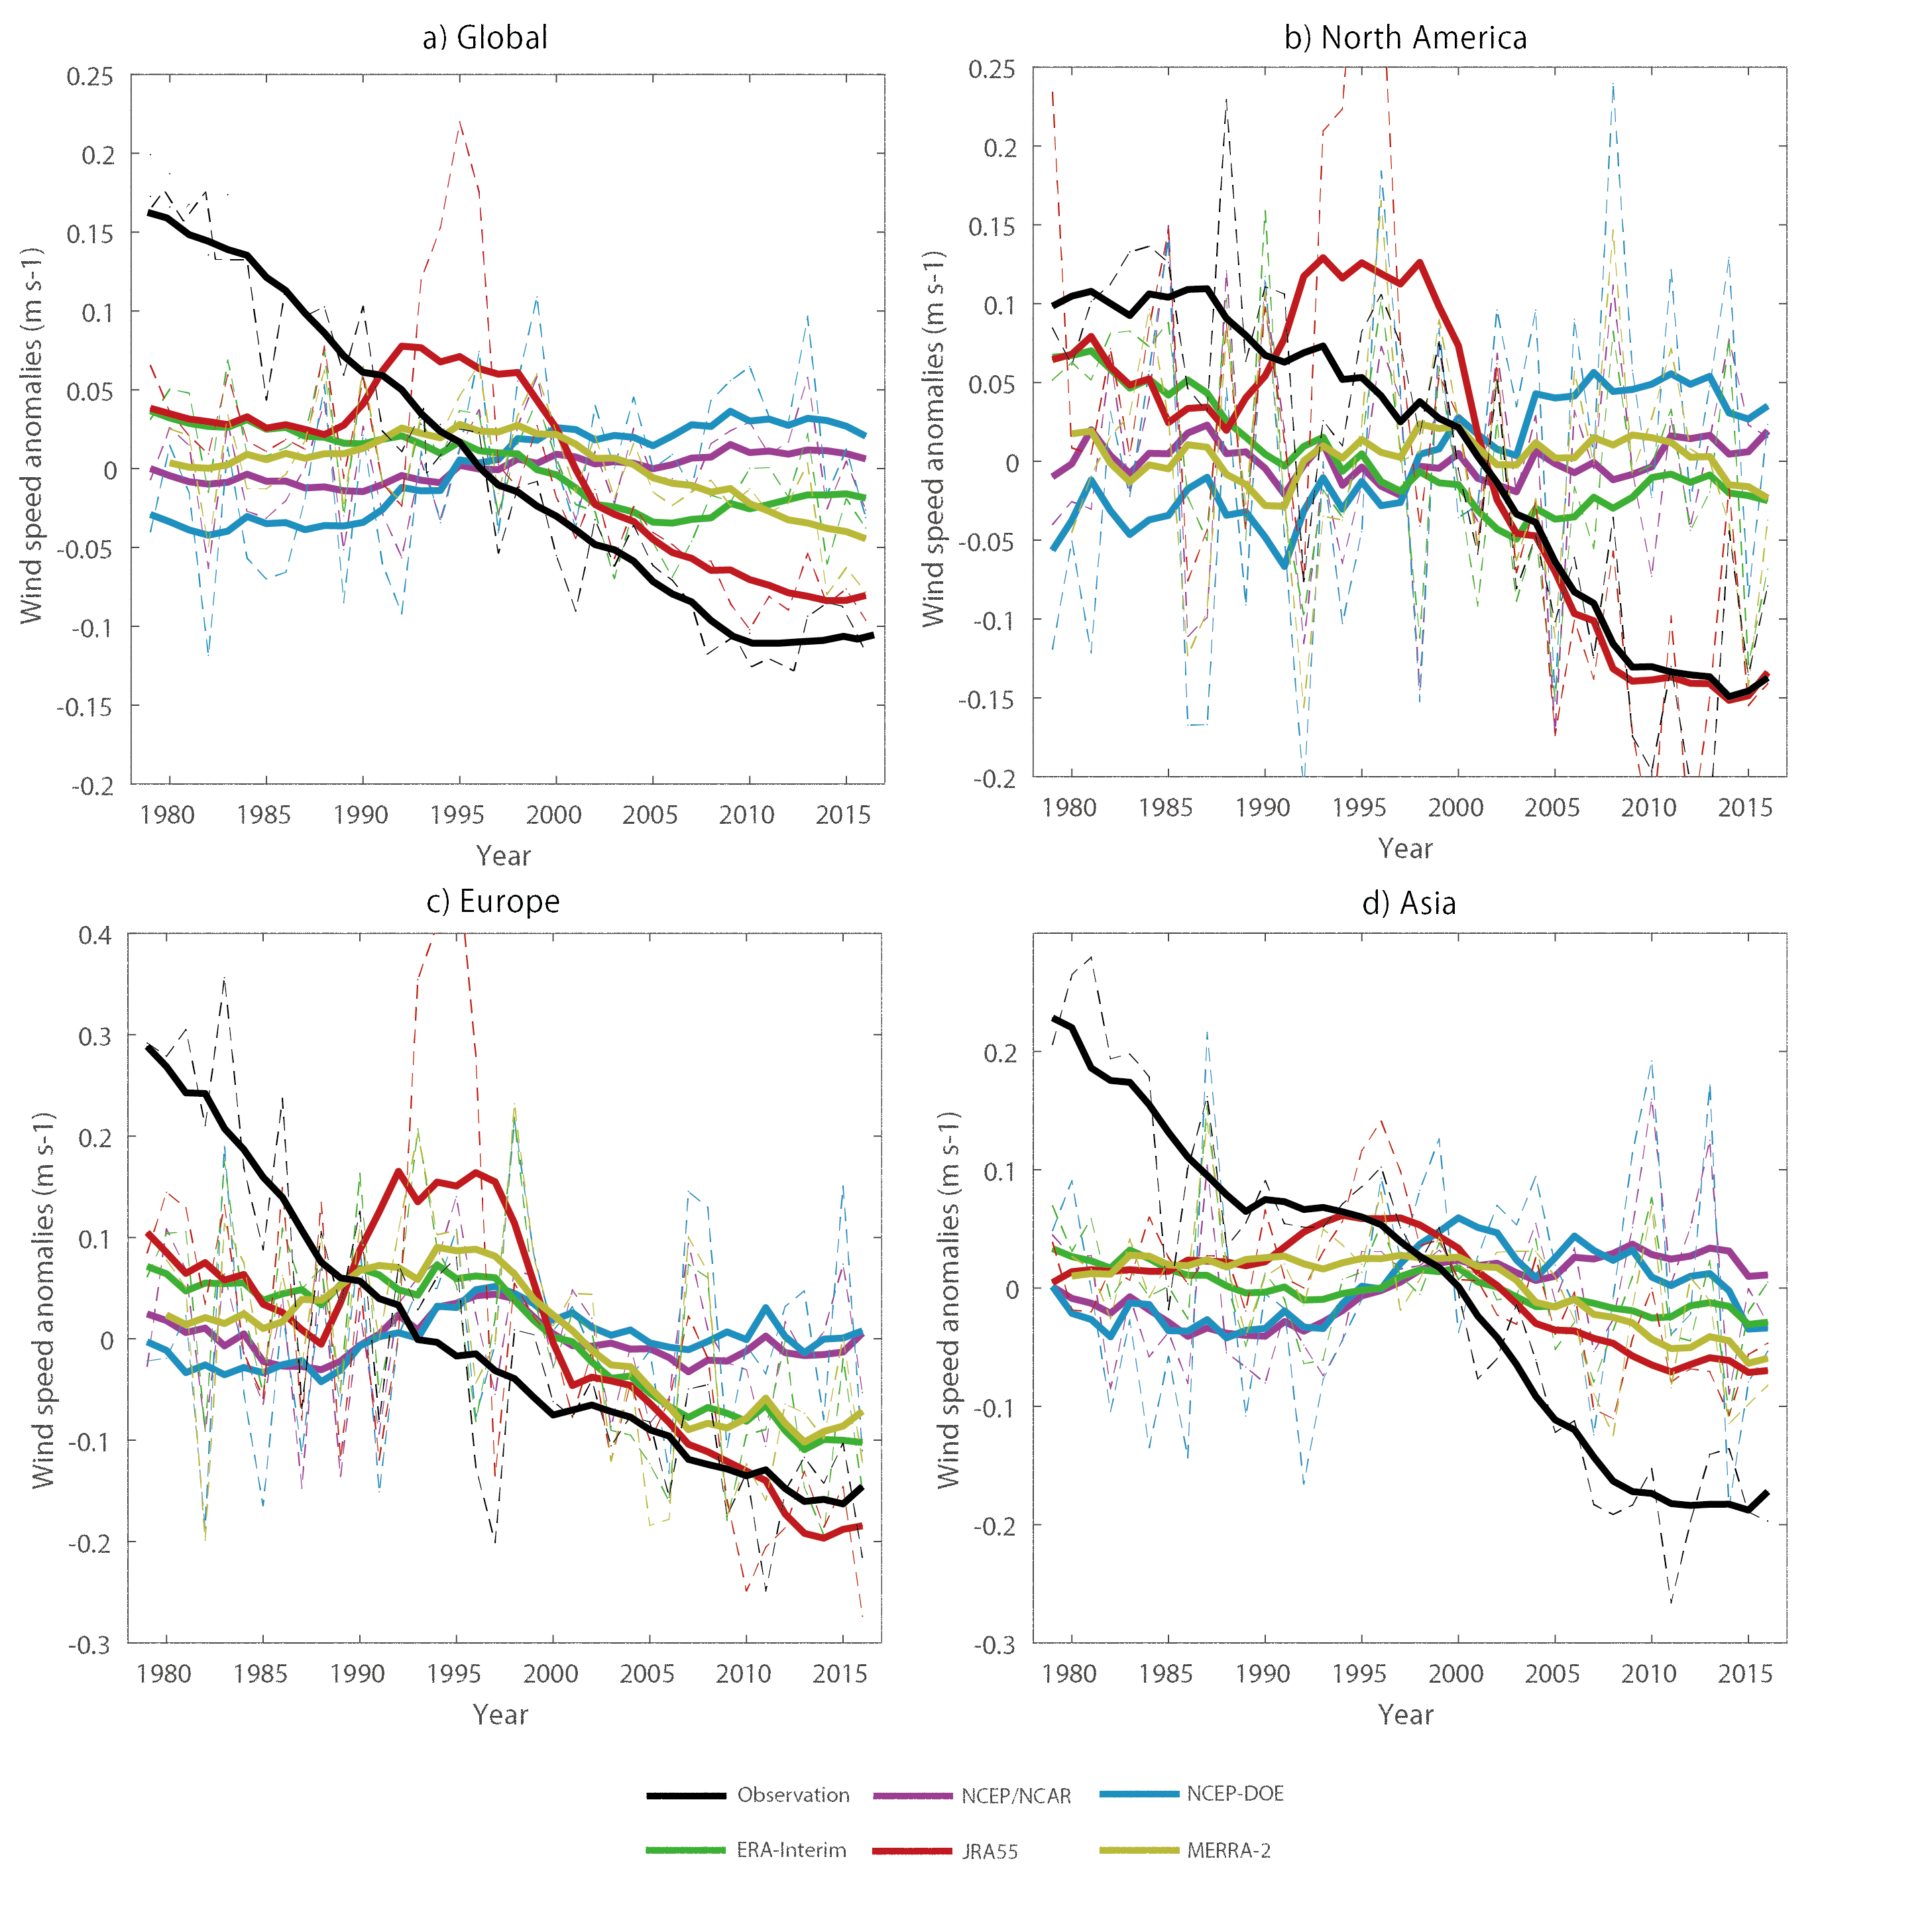
\includegraphics[width=0.9\textwidth]{风速年代际变化不确定性}
    \bicaption{观测及再分析资料风速年代际变化。a)全球,b)北美洲,c)欧洲,d)亚洲。虚线为年均值,实线为虚线9点平滑后的结果。}{Decadal changes of wind speed in observation and reanalysis data. a)Global, b)North America, c) Europe, d)Asia. Dash line is annual mean value, soild line is 9-point moving mean of dash line.}
    \label{fig:uncertaintywinddecadalchange}
\end{figure}

不同资料年平均风速年代际变化呈现的特点大不相同。全球平均来看,NCEP/NCAR和NCEP-DOE在1992-2000年期间风速有上升,1992年前和2000年后风速较为平稳;ERA-Interim在1995年前缓慢下降,1995-2005快速下降且下降速度与同期观测接近,2005年后风速回升;MERRA-2在1997年前风速上升而气候开始下降;JRA-55在1988年前缓慢下降,与同期ERA-Interim下降速度几乎一致,1988-2001年风速经历异常的极速上升,缓慢下降和异常的极速下降,后又快速下降,并且在2001-2007年下降速度与观测类似,其中1990年和2000年前后的极速上升和下降非常可能是由于JRA-55自身的错误所致,若将其扣除,JRA-55在1979-2016年间均呈下降趋势,2000年前下降较慢,其后下降较快(图 \ref{fig:uncertaintywinddecadalchange} a))。在北美洲,NCEP/NCAR和MERRA-2风速始终较为平稳;NCEP-DOE在1994年前和2005年后风速无显著趋势,1994-2005年间风速逐渐上升;ERA-Interim在2003年前风速下降而其后风速有上升趋势;JRA-55若扣除1990和2000前后的异常变化,表现为2000年前缓慢下降,2000-2010年快速下降,2010年后趋于平稳,与观测非常接近(图 \ref{fig:uncertaintywinddecadalchange} b))。在欧洲,NCEP/NCAR在1988年前风速缓慢下降,1988-1998风速上升,1988-2005风速再次缓慢下降,2005年后趋于平稳;NCEP-DOE与NCEP/NCAR年代际变化非常类似,不同之处在于NCEP-DOE在1988年前风速平稳;MERRA-2年代际变化也与NCEP/NCAR几乎一致除了1988-2005风速下降快于NCEP/NCAR;ERA-Interim在1995年前风速较为平稳,其后风速快速下降;JRA-55若扣除异常上升和下降,在1990年前快速下降,1990-2000趋于平稳,其后又快速下降(图 \ref{fig:uncertaintywinddecadalchange} c))。在亚洲,NCEP/NCAR在1998年前风速平稳,1998-2000风速上升,2000年后再次趋于平稳;NCEP-DOE前两个阶段与NCEP/NCAR接近,2000年后风速缓慢下降;ERA-Interim在1998年前风速缓慢下降,1995-2005缓慢上升后又缓慢下降,2005年后趋于平稳;MERRA-2在2000年前风速平稳,2000年后缓慢下降;JRA-55在1990年和2000年风速异常变化相对较小,扣除之后整体上体现为2000年前平稳,2000-2010缓慢下降,2010年后再次平稳(图 \ref{fig:uncertaintywinddecadalchange} d))。


\section{本章小结}

本章利用观测数据分析了全球(由于数据绝大多数来源于北半球,所以主要体现的是北半球的特征)以及北美洲、欧洲和亚洲分别的陆地地表风速长期趋势和趋势的年代际变化,并讨论了其中的不确定性,得到以下结论:

\begin{enumerate}

\item 陆地地表风速减弱是全球(主要是北半球)普遍发生的现象,中位数风速趋势为-0.081 $m ~ s^{-1}$每十年,北美洲、欧洲和亚洲分别为-0.075,-0.105和-0.075 $m ~ s^{-1}$每十年。

\item 风速趋势在不同百分位风速的表现有一定差别,总体来看,高百分位风速下降快于低百分位,但北美洲例外,其低百分位风速下降明显高于高百分位。

\item 风速趋势有明显的季节差异,总体来看,春季下降最快而夏季下降最慢。

\item 不同海拔的风速趋势有所差异,在北美洲和欧洲,海拔越高风速趋势越趋向于正,亚洲海拔与风速趋势无显著相关。

\item 风速趋势有显著的年代际变化。总体来看,风速下降发生在2010年前,之后风速趋于平稳。北美洲风速下降出现在1980至2010年间,其他时间风速平稳;欧洲近38年风速持续下降,2000年之后下降慢于之前;亚洲风速下降发生在1990年前和1997-2007年间,其他时间风速平稳。在不同季节上的风速年代际变化大多与年均值一致,欧洲夏季与其他季节差异明显,表现为2000年后显著增加。

\item 使用5套再分析资料得到的中位数风速趋势从0.022 $m ~ s^{-1}$每十年至-0.042 $m ~ s^{-1}$每十年不等,年代际变化也有较明显的不一致性,其中唯一同化了陆地地表风速观测的再分析资料JRA-55与观测的长期变化最为接近。
\end{enumerate}

%%  --------------------- chapter 3--------------------- %
\chapter{大气运动驱动力变化对陆地地表风速长期变化的影响}\label{chap:drivingforceonwind}

\section{引言}

第\ref{chap:SpatiotemporalCharacteristics}章全面分析了北半球陆地地表风速长期变化的时空特征,从本章开始探讨其背后的原因。如第一章所述,风速变化究其根本可以从大气运动驱动力的变化和大气运动阻力的变化两个方面来解释,本章将重点分析大气运动驱动力变化的影响。

垂直方向上来看,西风带大气运动的动量从高层向低层传递,并在地面被摩擦作用消耗掉。因此,了解高层大气风速变化对理解地表风速变化的原因非常重要。之前少有研究涉及风速的垂直变化,\citet{vautard2010northern}发现1979-2008年间北半球高层风速没有出现像地表风速一样的普遍减弱的情况,\citet{lin2013observed}发现1960-2009年间中国高层风速与地表风速变化存在一定的相似性,因而地表风速变化可以一定程度上由高层变化解释。本章将首先全面分析北半球自由大气各个层次的长期变化特征以及它们与地表风速长期变化的区别和联系。

气压场的变化与大气运动驱动力变化直接相关。\citet{zhang2019increase}利用简化的动力学模型分析发现海平面气压场变化是1970年以来北半球陆地地表风速月变化的主导因素,\citet{wu2016estimating}发现海平面气压场可以很大程度上解释中国东部地区陆地地表风速的季节和年际变率。本章对全球冬季和夏季的海平面气压场长期趋势进行了分析,探究大尺度气压场变化对于陆地地表风速的影响。

环流系统的变化是大气运动驱动力变化的重要反映,大尺度海温同样会影响大气驱动力,而环流系统与大尺度海温两者的变化又通常相互联系。例如,NAO的定义为500hPa位势高度场进行旋转经验正交分解(REOF)的第一模态,反映的是冰岛低压和亚速尔高压的强弱交替如跷跷板一般的变化\citep{wallace1981teleconnections}。诸多研究表明,NAO变率可以对欧洲地表风速产生显著影响\citep{beniston2005mountain, earl20131980–2010},同时,NAO变率受到大西洋海温的影响\citep{frankignoul2005observed}。与NAO类似,AO的变率也会影响大尺度陆地地表风速\citep{chen2013wind},也与海温有一定联系\citep{yasunaka2002regime}。大尺度海温模态太平洋年代际振荡(PDO)也被认为与大尺度陆地地表风速变化有一定联系\citep{fu2011temporal}。本章同样分析了环流系统及大尺度海温变化对于北半球陆地地表风速的影响。

\section{资料和方法}

本章研究使用了以下数据集:

IGRA V2全球探空数据集\citep{durre2006overview}由NOAA制作,包含全球超过2700个探空站点的观测数据。此数据集进行了一系列质量控制,对可疑和错误数据进行了标记。本章研究选取了1979-2016年850 hPa、700 hPa、500 hPa和200 hPa风速数据进行分析。为了保证数据质量,剔除了所有被标记为可疑和错误的数据;剔除了1981年1月的所有数据,因为此时间段数据有较大问题\citep{vautard2010northern};若某站点在某年内在某个层次任意一个季节内有记录天数少于45天,则移除此站点当年在此层次所有数据,若此站点在此层次有记录年数少于20年,则移除此层次所有数据。经过质量控制后,850 hPa、700 hPa、500 hPa和200 hPa分别剩余558、578、559和527个站点。本章中对流层风速相关分析均是基于此数据集。

\href{https://b2share.eudat.eu/records/159158152f4d4be79559e2f3f6b1a410}{高塔观测数据集}由巴塞罗那超算中心(BSC)制作,包含全球183个观测塔数据。此数据集针对风速进行了18项数据质量检测,删除了错误数据。此数据集中包含的观测序列大多时间较短,在北美洲仅有5个站点有30年以上的观测长度,因而选择此5个站点分析地表以上30 - 50 m高度风速变化。由于此5个站点均不包含10 m标准高度的风速观测,因而选取HadISD v3(\citet{dunn2012hadisd:},此数据集由第二章使用到的NCEI-ISD整理而成,不同于NCEI-ISD以时间为单位存储,即每月的数据存储在一个文件中,此套数据以站点为单位存储,即每个站点的数据存储在一个文件中,更易于少量站点数据的读取)中与它们距离最近的站点风速进行对比。

HadSLP2r全球海平面气压观测数据集\citep{allan2006a}由哈德莱中心(Hadley Centre)制作,包含1850年至今全球海平面气压场数据。此数据集使用ICOADS海洋观测数据和2228个陆地观测站数据,最终制作成$5 \times 5$度格点数据,并由NOAA PSD转换成NetCDF格式提供\href{https://www.esrl.noaa.gov/psd/gcos_wgsp/Gridded/data.hadslp2.html}{下载} 。此套数据进行了一系列质量控制减少人为误差造成的影响。本章使用此数据集1979-2016年数据分析全球海平面气压场的长期趋势。

HadSST3全球海表温度观测数据集\citep{kennedy2011reassessing1,kennedy2011reassessing2}由哈德莱中心制作,包含1850年至今全球海表温度。此数据集使用ICOADS、GST和ERDDAP海洋观测数据,制作成$5 \times 5$度格点数据。此数据集进行了一系列质量控制减少人为误差造成的影响。本章使用此数据集1979-2016年数据分析其与陆地地表风速序列的相关性。

中国气象局国家气候中心\href{https://cmdp.ncc-cma.net/Monitoring/cn_index_130.php}{百项气候系统指数集}整理了130项大气环流、海温和其他指数,其中涵盖了厄尔尼诺-南方涛动(ENSO),NAO、AO、PDO等环流和海温指数。经过检查,发现其中AO指数与其他研究存在较大差别,因而没有使用,转而使用NOAA计算的\href{https://www.ncdc.noaa.gov/teleconnections/ao/}{AO指数}。本章中使用这些环流和海温指数与陆地地表风速进行对比,以找出它们之间的联系。

本章中计算线性趋势和统计显著性检验的方法与第二章相同。相关系数计算使用Pearson相关系数,计算方法如下:

\begin{equation} \label{eq:pearsoncorr}
r = \frac{cov \left(A, ~ B \right)}{\sigma_{A}\sigma_{B}}
\end{equation} ~\\
其中,$cov \left(A, ~ B \right)$为序列$A$、$B$的协方差,$\sigma_{A}$、$\sigma_{B}$分别为$A$、$B$的标准差。

\section{对流层风速长期变化}

\subsection{对流层风速长期线性趋势}

\begin{figure}[!htbp]
    \centering
    \includegraphics[width=0.75\textwidth]{对流层风速趋势}
    \bicaption{对流层风速趋势($m ~ s^{-1}$每十年)。a)200 hPa,b)500 hPa,c)700 hPa,d)850 hPa,e)地面。}{Troposphere wind speed trends (in $m ~ s^{-1} ~ decade^{-1}$). a)200 hPa, b)500 hPa, c)600 hPa, d)850 hPa, e)Surface.}
    \label{fig:tropospherewindtrend}
\end{figure}

\begin{figure}[!b]
    \centering
    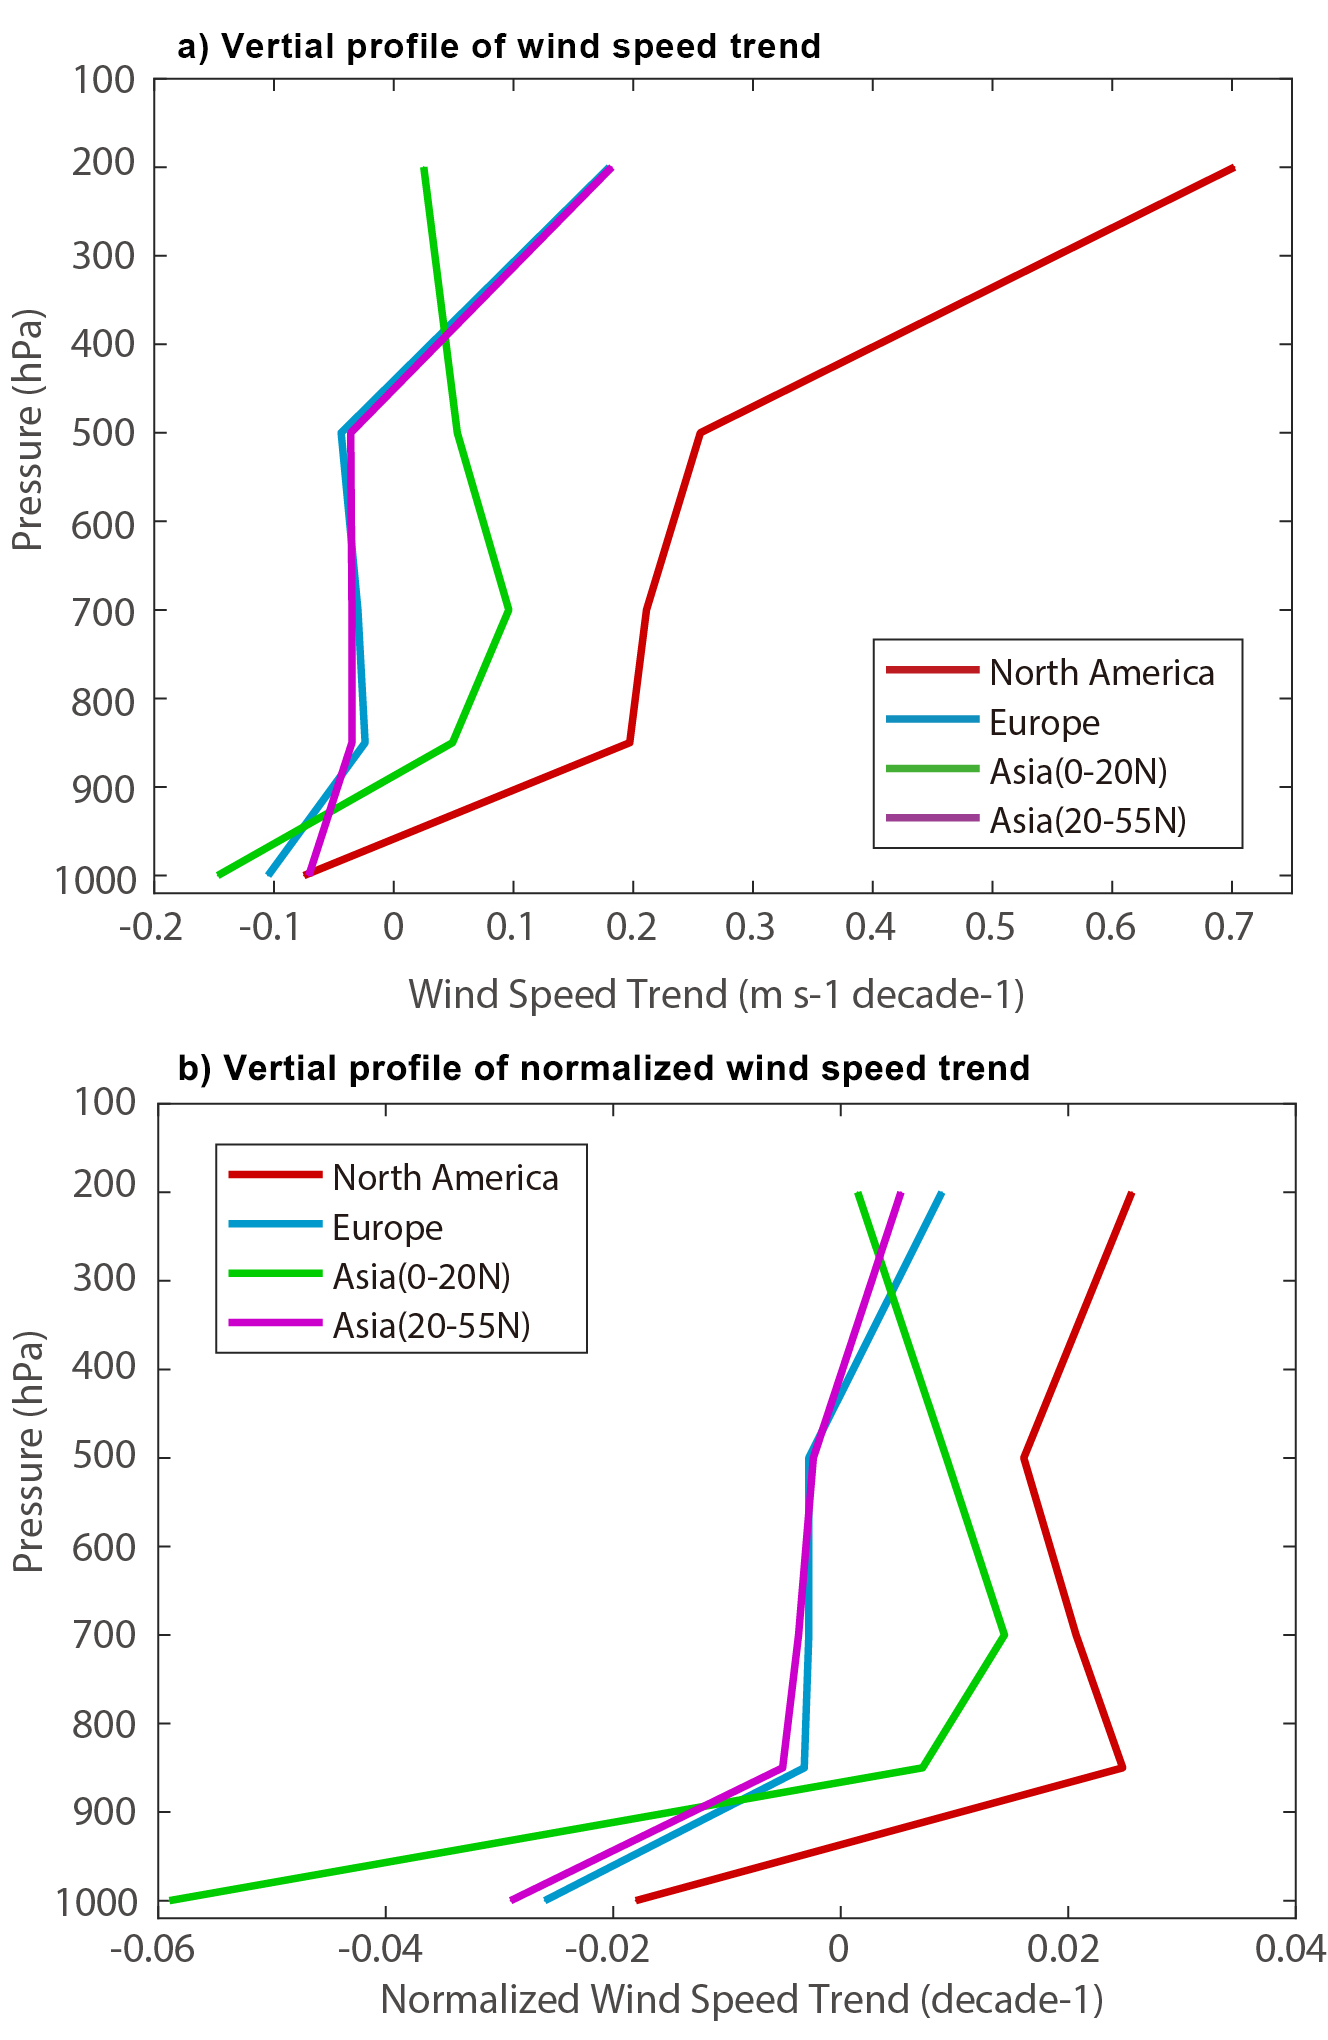
\includegraphics[width=0.65\textwidth]{对流层中位数风速趋势}
    \bicaption{对流层中位数风速趋势($m ~ s^{-1}$每十年)。a)原始风速趋势,b)归一化风速趋势,即原始风速趋势/平均风速。红线为北美洲,蓝线为欧洲,绿线为亚洲低纬度地区(0-20 N),紫线为亚洲中纬度地区(20-55 N)。}{Troposphere median wind speed trends (in $m ~ s^{-1} ~ decade^{-1}$). a) Original wind speed trends. b) Normalized wind speed trends, i.e. original wind speed trends divided by climatological wind speed. Red line denotes North America, blue denotes Europe, green denotes Asian low altitude area (0-20 N), purple denotes Asian mid-latitude area (20-55 N). }
    \label{fig:tropospheremedianwindtrend}
\end{figure}


使用IGRA V2探空风速数据计算了对流层850 hPa、700 hPa、500 hPa和200 hPa长期趋势,分别代表对流层低层、中低层、中层和高层的状况,发现风速的长期趋势在垂直方向上有很大的不均匀性,地表风速减弱最为剧烈,而对流层风速有微弱减小甚至增加(图 \ref{fig:tropospheremedianwindtrend})。在北美洲,地表风速普遍减小,而自由大气风速在各个层次均出现上升(图 \ref{fig:tropospherewindtrend})。为了进一步探究风速开始增加的高度,使用了5个观测塔资料(观测塔信息如图 \ref{fig:talltower}和表(观测塔与附近地面站点信息))分析,发现高度在40 m左右的5个观测塔风速均呈显著上升,相比之下,与其最邻近的地面站点有2个风速显著上升,2个风速显著下降,1个无明显趋势(图 \ref{fig:talltowerwindtrend1}, 图 \ref{fig:talltowerwindtrend2})。由此可以推测,在地面附近几十米的高度就出现了风速普遍上升的情况。在欧洲,地表风速同样普遍下降,而850 – 500 hPa伊比利亚半岛风速出现上升,欧洲其他大部分地区风速普遍下降,200 hPa欧洲风速普遍上升。总体来看,欧洲各层次中位数风速中地表风速下降最快,约为 -0.1 $m ~ s^{-1}$每十年,850  hPa和700 hPa风速微弱下降,趋势在 -0.02 \textasciitilde -0.03 $m ~ s^{-1}$ 每十年,200 hPa风速上升,趋势为0.17 $m ~ s^{-1}$每十年。如果考虑到高层平均风速比底层大得多,归一化后的风速趋势只有在地表较为显著(图 \ref{fig:tropospherewindtrend},图 \ref{fig:tropospheremedianwindtrend})。因为亚洲站点跨越热带和中纬度两个气候带,将其以20 N为界分为两个部分进行分析,其中亚洲低纬度地区地表风速普遍下降,850和700 hPa开始出现较多风速增加站点,500和200 hPa相比对流层底层有风速增加站点减小。总体来看,风速在地表减小(-0.15 $m ~ s^{-1}$每十年),在对流层由低层到高层风速增加,增加幅度先增加再减小,200 hPa风速变化接近为零。归一化风速趋势上,亚洲低纬度风速下降明显快于北美洲、欧洲和亚洲中纬度地区,达到-6\% 每十年(图 \ref{fig:tropospherewindtrend},图 \ref{fig:tropospheremedianwindtrend})。亚洲中纬度地区,除中部地区风速上升,中国其他大部分地区地表风速普遍下降,日本地表风速上升的下降站点相当;850 hPa上,中国大部分地区风速微弱下降或无明显变化,日本风速微弱上升或无明显变化;700和500 hPa上,中国东部地区风速微弱下降或无明显变化,中国西北和中亚风速上升,日本风速下降;200 hPa上,除中国东南地区外,亚洲中纬度大部分地区风速普遍上升。总体来看,亚洲中纬度风速在地面下降较快(-0.75 $m ~ s^{-1}$每十年),850和700 hPa风速微弱下降(-0.25 $m ~ s^{-1}$每十年),200 hPa风速上升(0.17 $m ~ s^{-1}$每十年),归一化风速趋势只有在地表较为明显(图 \ref{fig:tropospherewindtrend},图 \ref{fig:tropospheremedianwindtrend})。


\begin{figure}[!htbp]
    \centering
    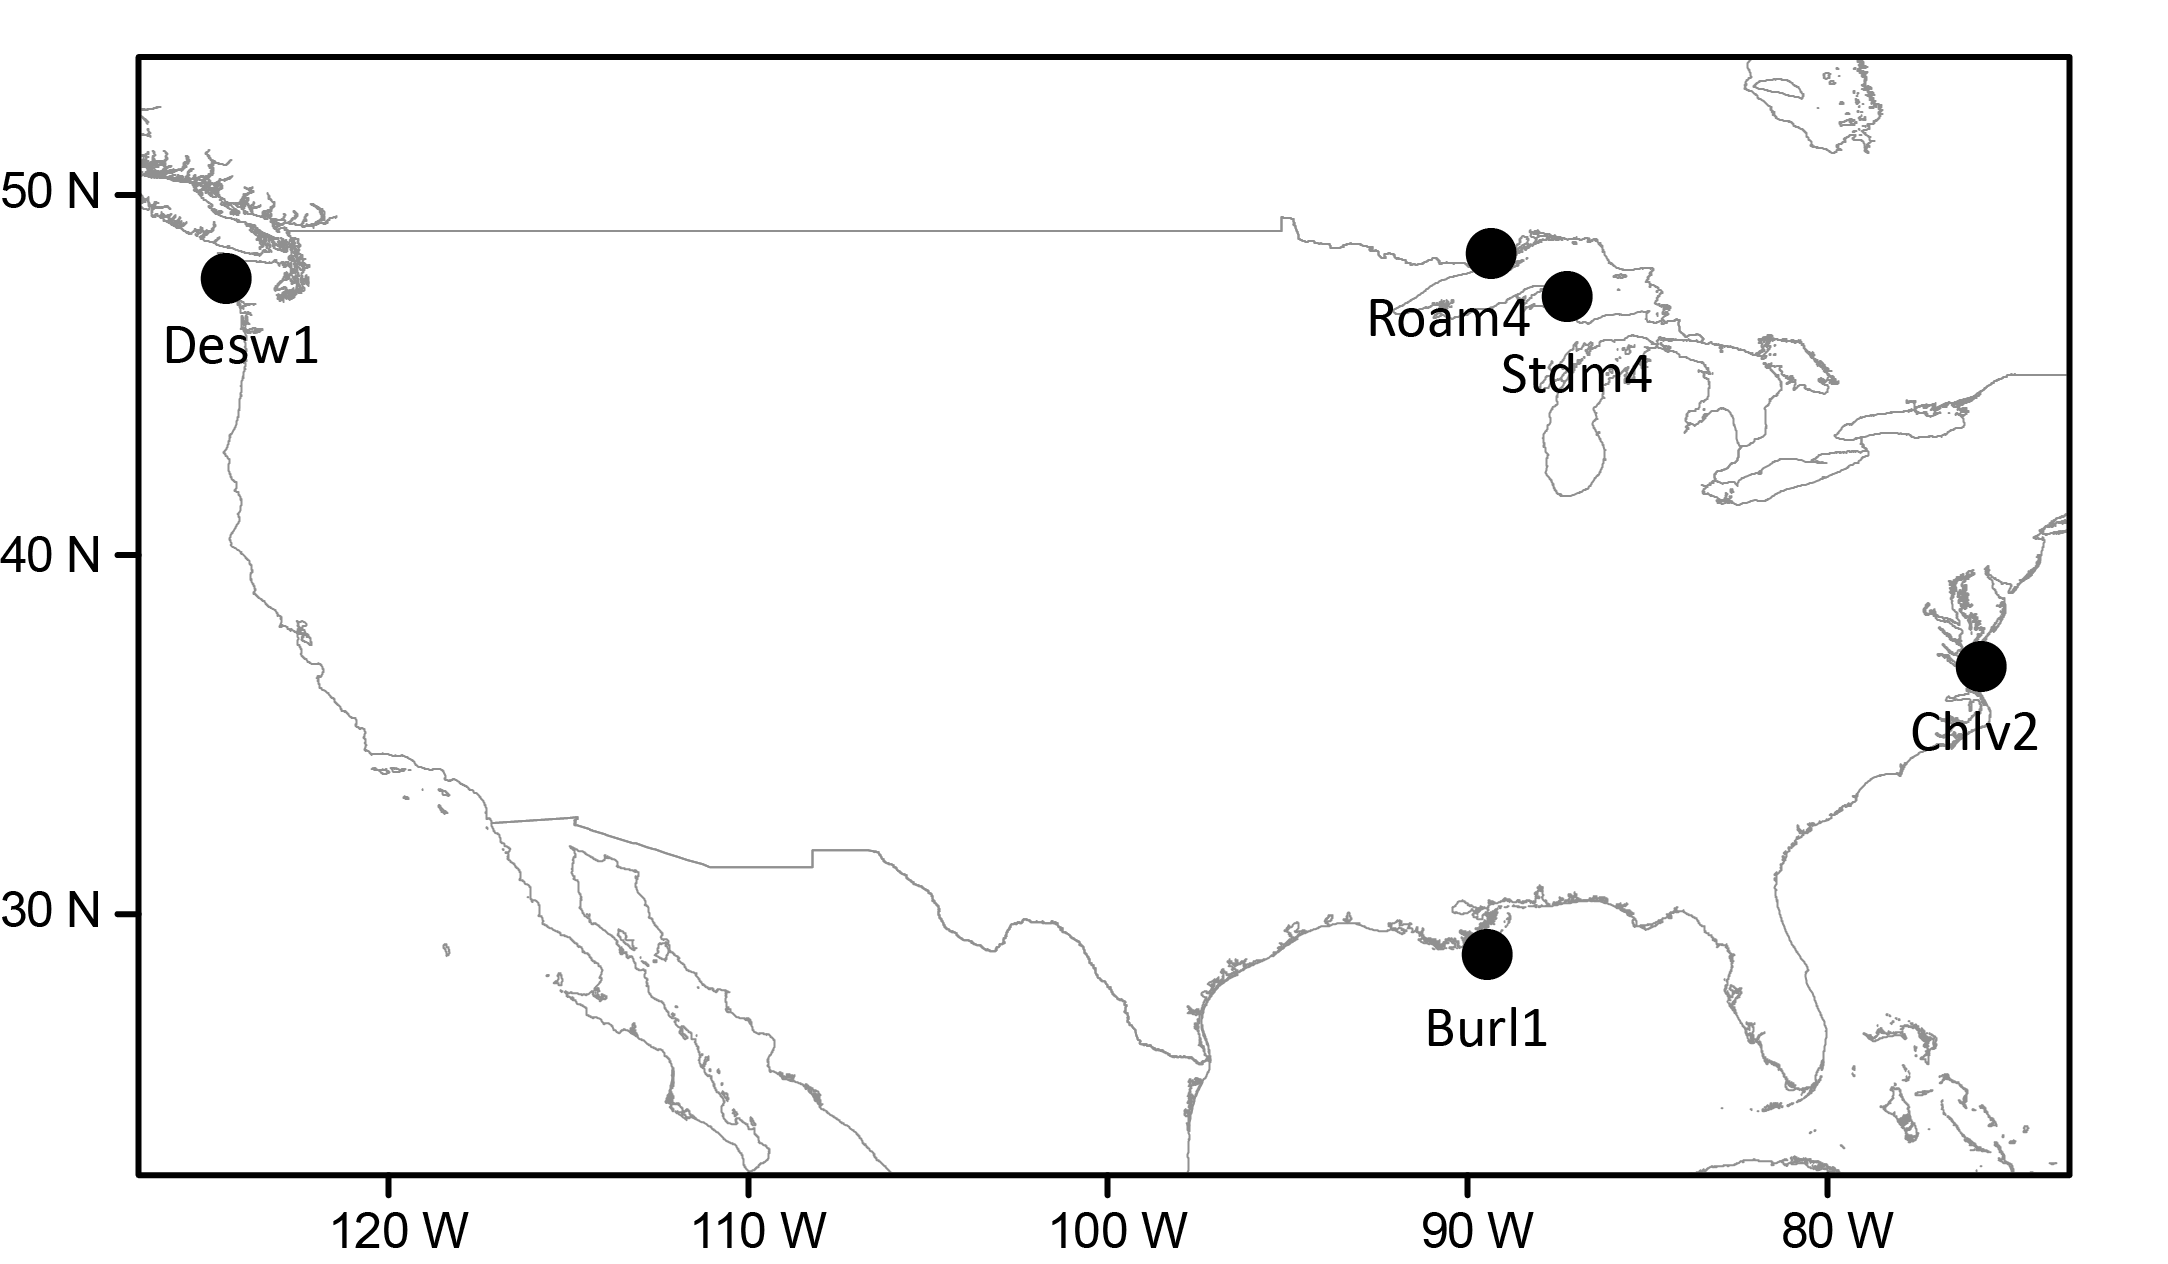
\includegraphics[width=0.75\textwidth]{北美观测塔分布}
    \bicaption{北美观测塔分布}{Locations of observation tower in North America}
    \label{fig:talltower}
\end{figure}

\begin{table}[!htbp]
    \bicaption{观测塔与附近地面站点信息}{Description of observation towers and the surface observation stations close to them}
    \label{tab:stationinfo}
    \centering
    \footnotesize% fontsize
    \setlength{\tabcolsep}{3 pt}% column separation
    \renewcommand{\arraystretch}{1.0}%row space 
    \begin{tabular}{lccccccc}
        \hline
        观测塔名称 & 观测塔经度 & 观测塔纬度 & 风速观测高度 & 距离最近地面 & 站点经度 & 站点纬度 & 风速观测高度 \\
        & & & (地面以上 m)& 站点号 & & &(地面以上 m)\\
        %\cline{2-9}% partial hline from column i to column j
        \hline
        Burl1 & -89.43 & 28.90 & 38 & 994010 & -89.43 & 28.91 & 10 \\
        Chlv2 & -75.71 & 36.91 & 43 & 723075 & -76.03 & 36.82 & 10 \\
        Desw1 & -124.49 & 47.68 & 31 & 727970 & -124.55 & 47.94 & 10 \\
        Roam4 & -89.31 & 47.87 & 47 & 717490 & -89.33 & 48.37 & 10 \\
        Stdm4 & -87.23 & 47.18 & 35 & 727440 & -88.49 & 47.17 & 10 \\ 
        \hline
    \end{tabular}
\end{table}

\begin{figure}[!htbp]
    \centering
    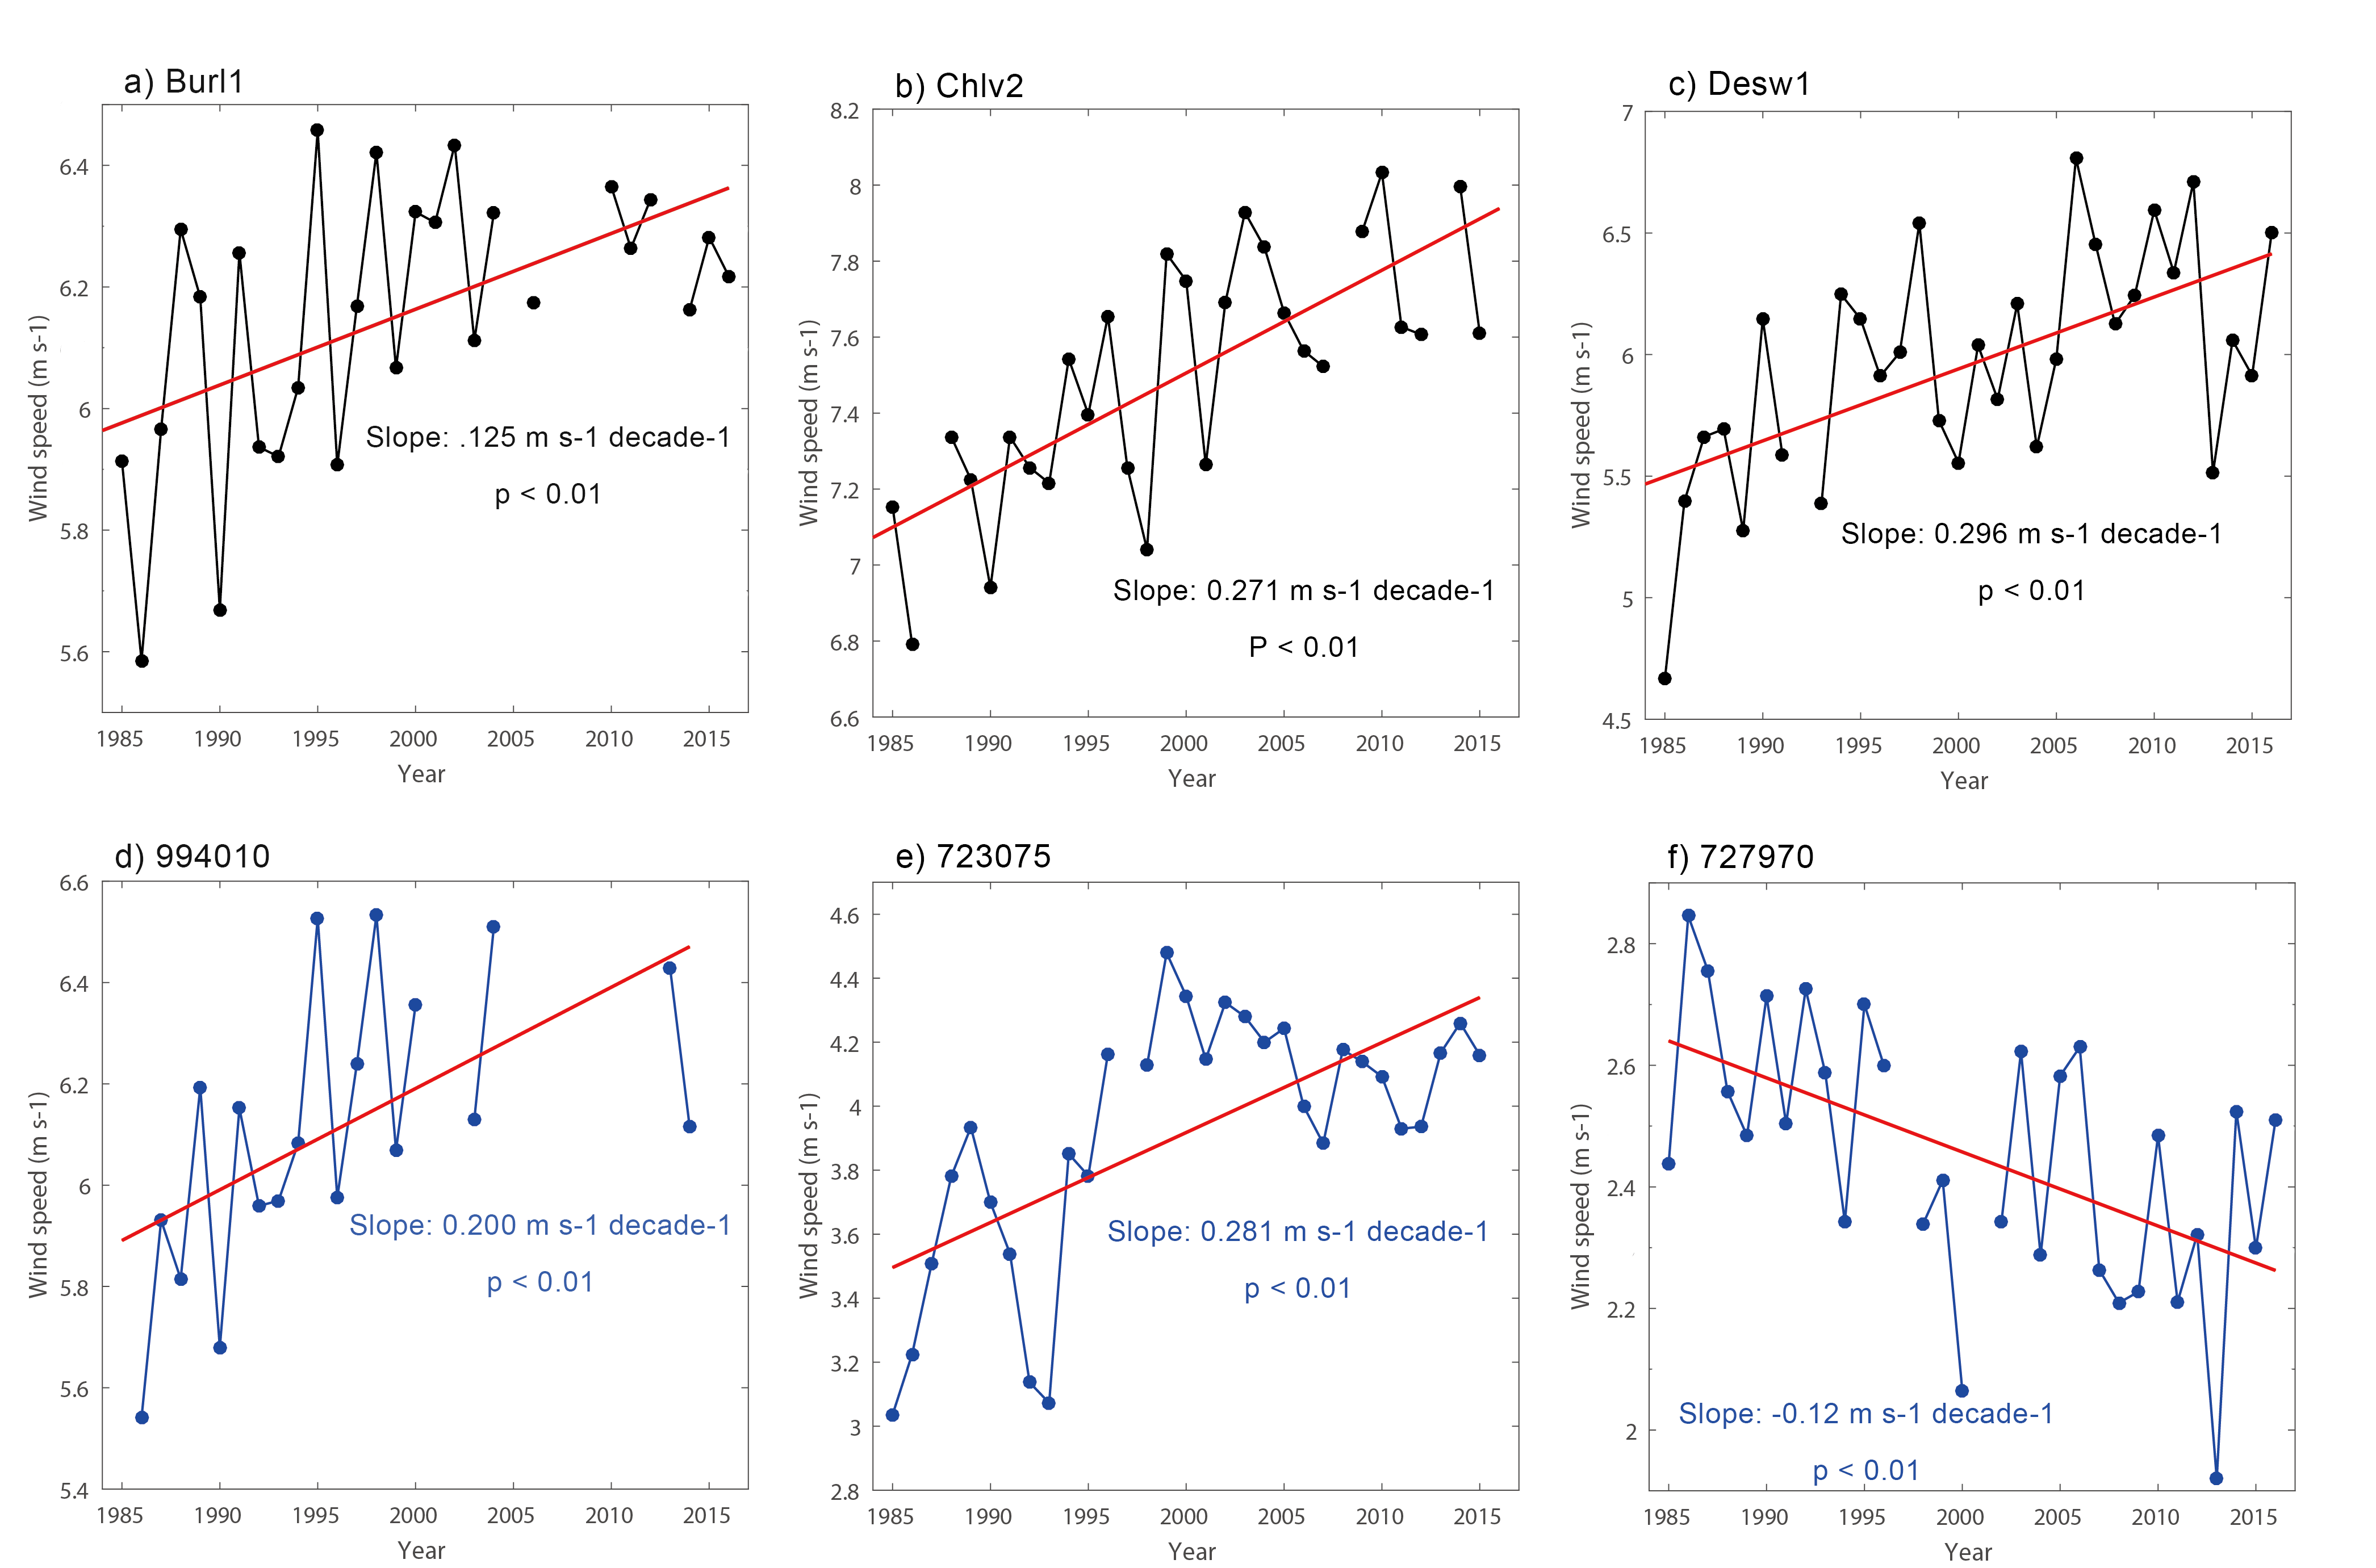
\includegraphics[width=1\textwidth]{北美观测塔风速趋势1}
    \bicaption{北美观测塔风速趋势(第一部分)。d)994010、e)723075、f)727970分别为距离观测塔a)Burl1、b)Chlv2、c)Desw1最近的地面观测站点。}{Wind speed trends of observation tower in North America (part 1). d)994010, e)723075, f)727970 are surface observation stations closest to a)Burl1, b)Chlv2, c)Desw1, respectively.}
    \label{fig:talltowerwindtrend1}
\end{figure}

\begin{figure}[!t]
    \centering
    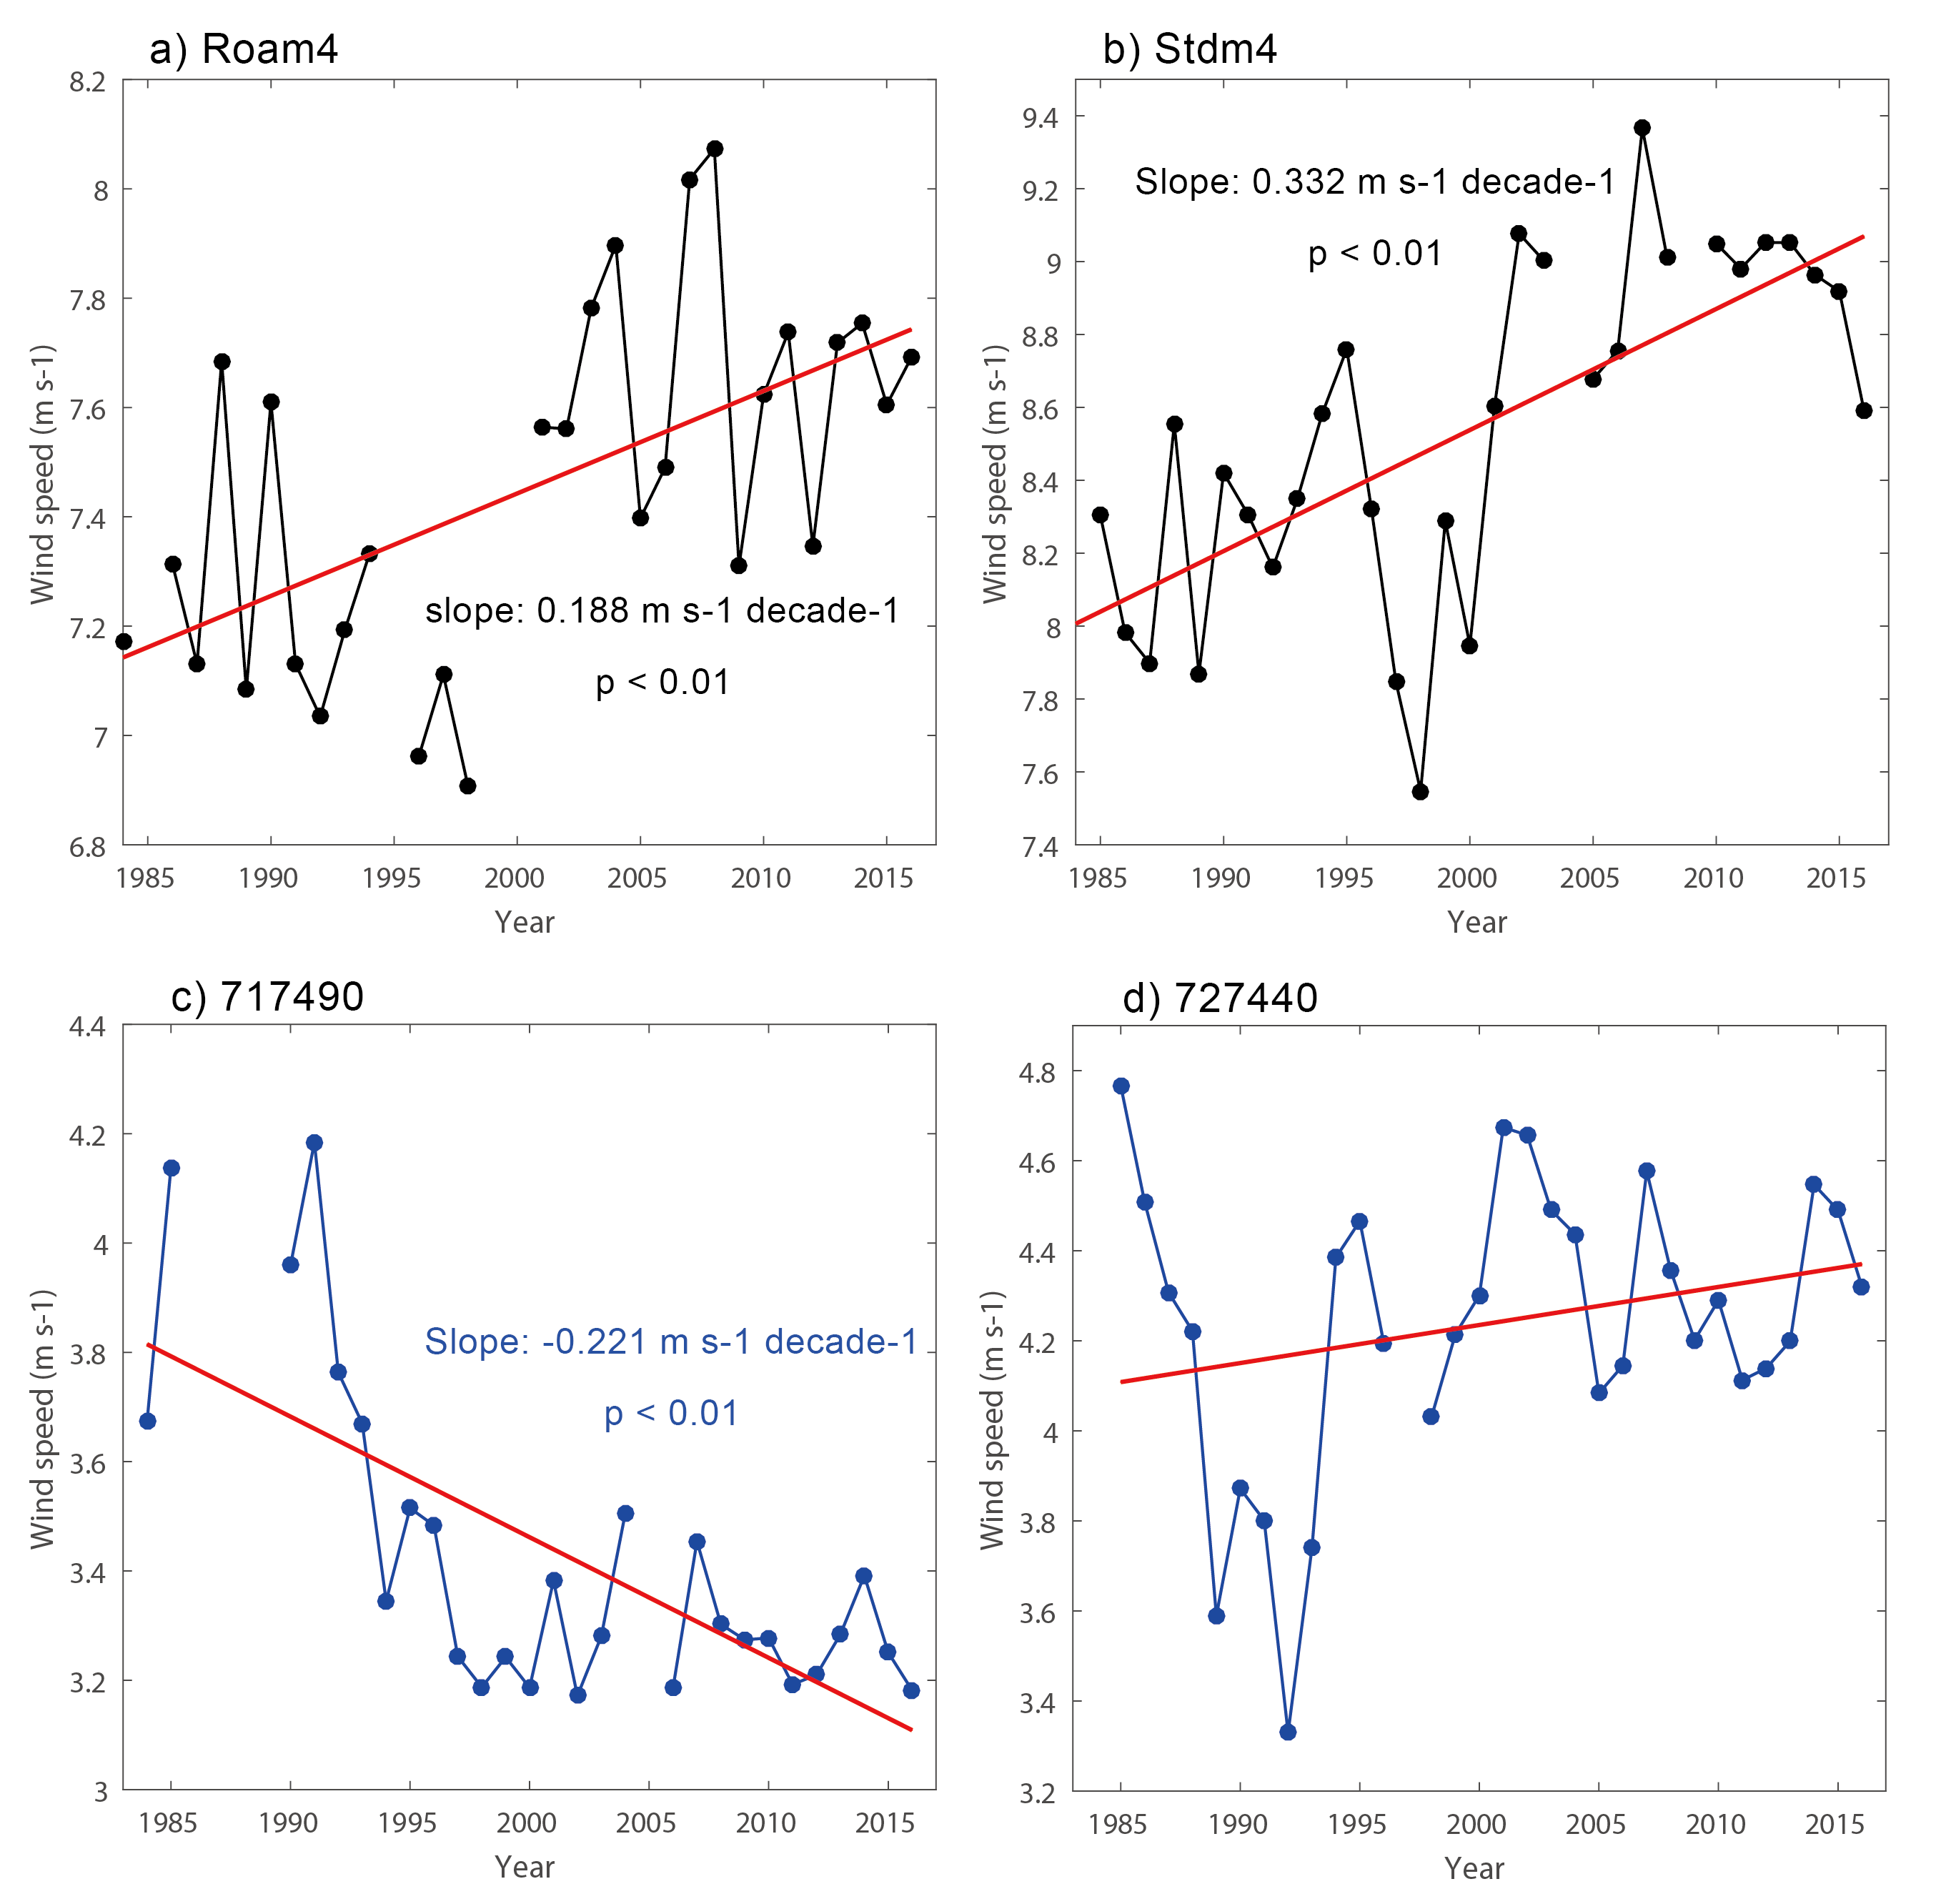
\includegraphics[width=0.65\textwidth]{北美观测塔风速趋势2}
    \bicaption{北美观测塔风速趋势(第二部分)。c)717490、d)727440分别为距离观测塔a)Roam4、b)Stdm4最近的地面观测站点。}{Wind speed trends of observation tower in North America (part 2). c)717490、d)727440 are surface observation stations closest to a)Roam4、b)Stdm4, respectively.}
    \label{fig:talltowerwindtrend2}
\end{figure}

\subsection{对流层风速年代际变化}

全球平均来看,地表风速在2007年前迅速下降,气候趋于平稳;850 hPa风速先上升(1990年前),后下降(1990-2000),再上升(2000年后)三个阶段;700 hPa在2005年前与850 hPa变化类似,2005年后趋于平稳;500 hPa风速在1995年前快速上升,气候缓慢下降;200 hPa风速1990年前缓慢下降,1990-2000快速上升,其后又缓慢下降(图 \ref{fig:globaltroposhereevolution})。在北美洲,地表风速经历了1987年前平稳时期,1987-2000缓慢下降时期,2000-2010快速下降时期和2010年后平稳时期;850和700 hPa,风速表现为1995年前快速上升时期,1995-2005缓慢上升时期和2005年后缓慢下降时期;500 hPa风速在1995年前快速上升,1995-2003缓慢下降,2003-2013又快速上升,其后在此出现下降;200 hPa风速在1988年前缓慢下降,1988-1995快速上升,1995-2005趋于平稳,2005年后再次快速上升(图 \ref{fig:NAtroposhereevolution})。在欧洲,地表风速1990年前快速下降,1990-2000中速下降,2000年后慢速下降;850和700 hPa年代际变化较为类似,均在1985年前无明显变化,1985-1993上升,1993-2003下降,不同之处在于850 hPa在2003年后又开始缓慢上升,而700 hPa趋于平稳;500和200 hPa,风速均经历了1990年前平稳时期,1990-2000年上升时期,2000-2010年下降时期和2010年后再次缓慢上升时期(图 \ref{fig:EUtroposhereevolution})。在亚洲低纬度地区,地表风速在1987年前快速下降,1987-1995年微弱上升,之后又快速下降;850 hPa在1990年前微弱上升,之后快速下降直到2000年,其后2000-2010再次缓慢上升,后又下降;700 hPa年代际变化不明显;500 hPa风速在1990年前缓慢上升,1990-2000缓慢下降,2000-2010快速上升,其后缓慢下降;200 hPa风速以2000年为界,前期风速上升,后期风速下降(图 \ref{fig:ASlowtroposhereevolution})。在亚洲中纬度地区,地表风速在1990年前快速下降,1990-1997年趋于平稳,1997-2007再次快速下降,2007年后再次趋于平稳;850 hPa和700 hPa风速变化都以1990和2000为界分为三个时期,850 hPa风速在这三个时期表现分别为平稳、下降和上升,而700 hPa表现为缓慢下降,快速下降和上升;500 hPa风速没有表现出明显年代际变化;200 hPa风速仅在1993-2003有一段上升时期,之前和之后风速均较为平稳(图 \ref{fig:ASmidtroposhereevolution})。

\begin{figure}[!htbp]
    \centering
    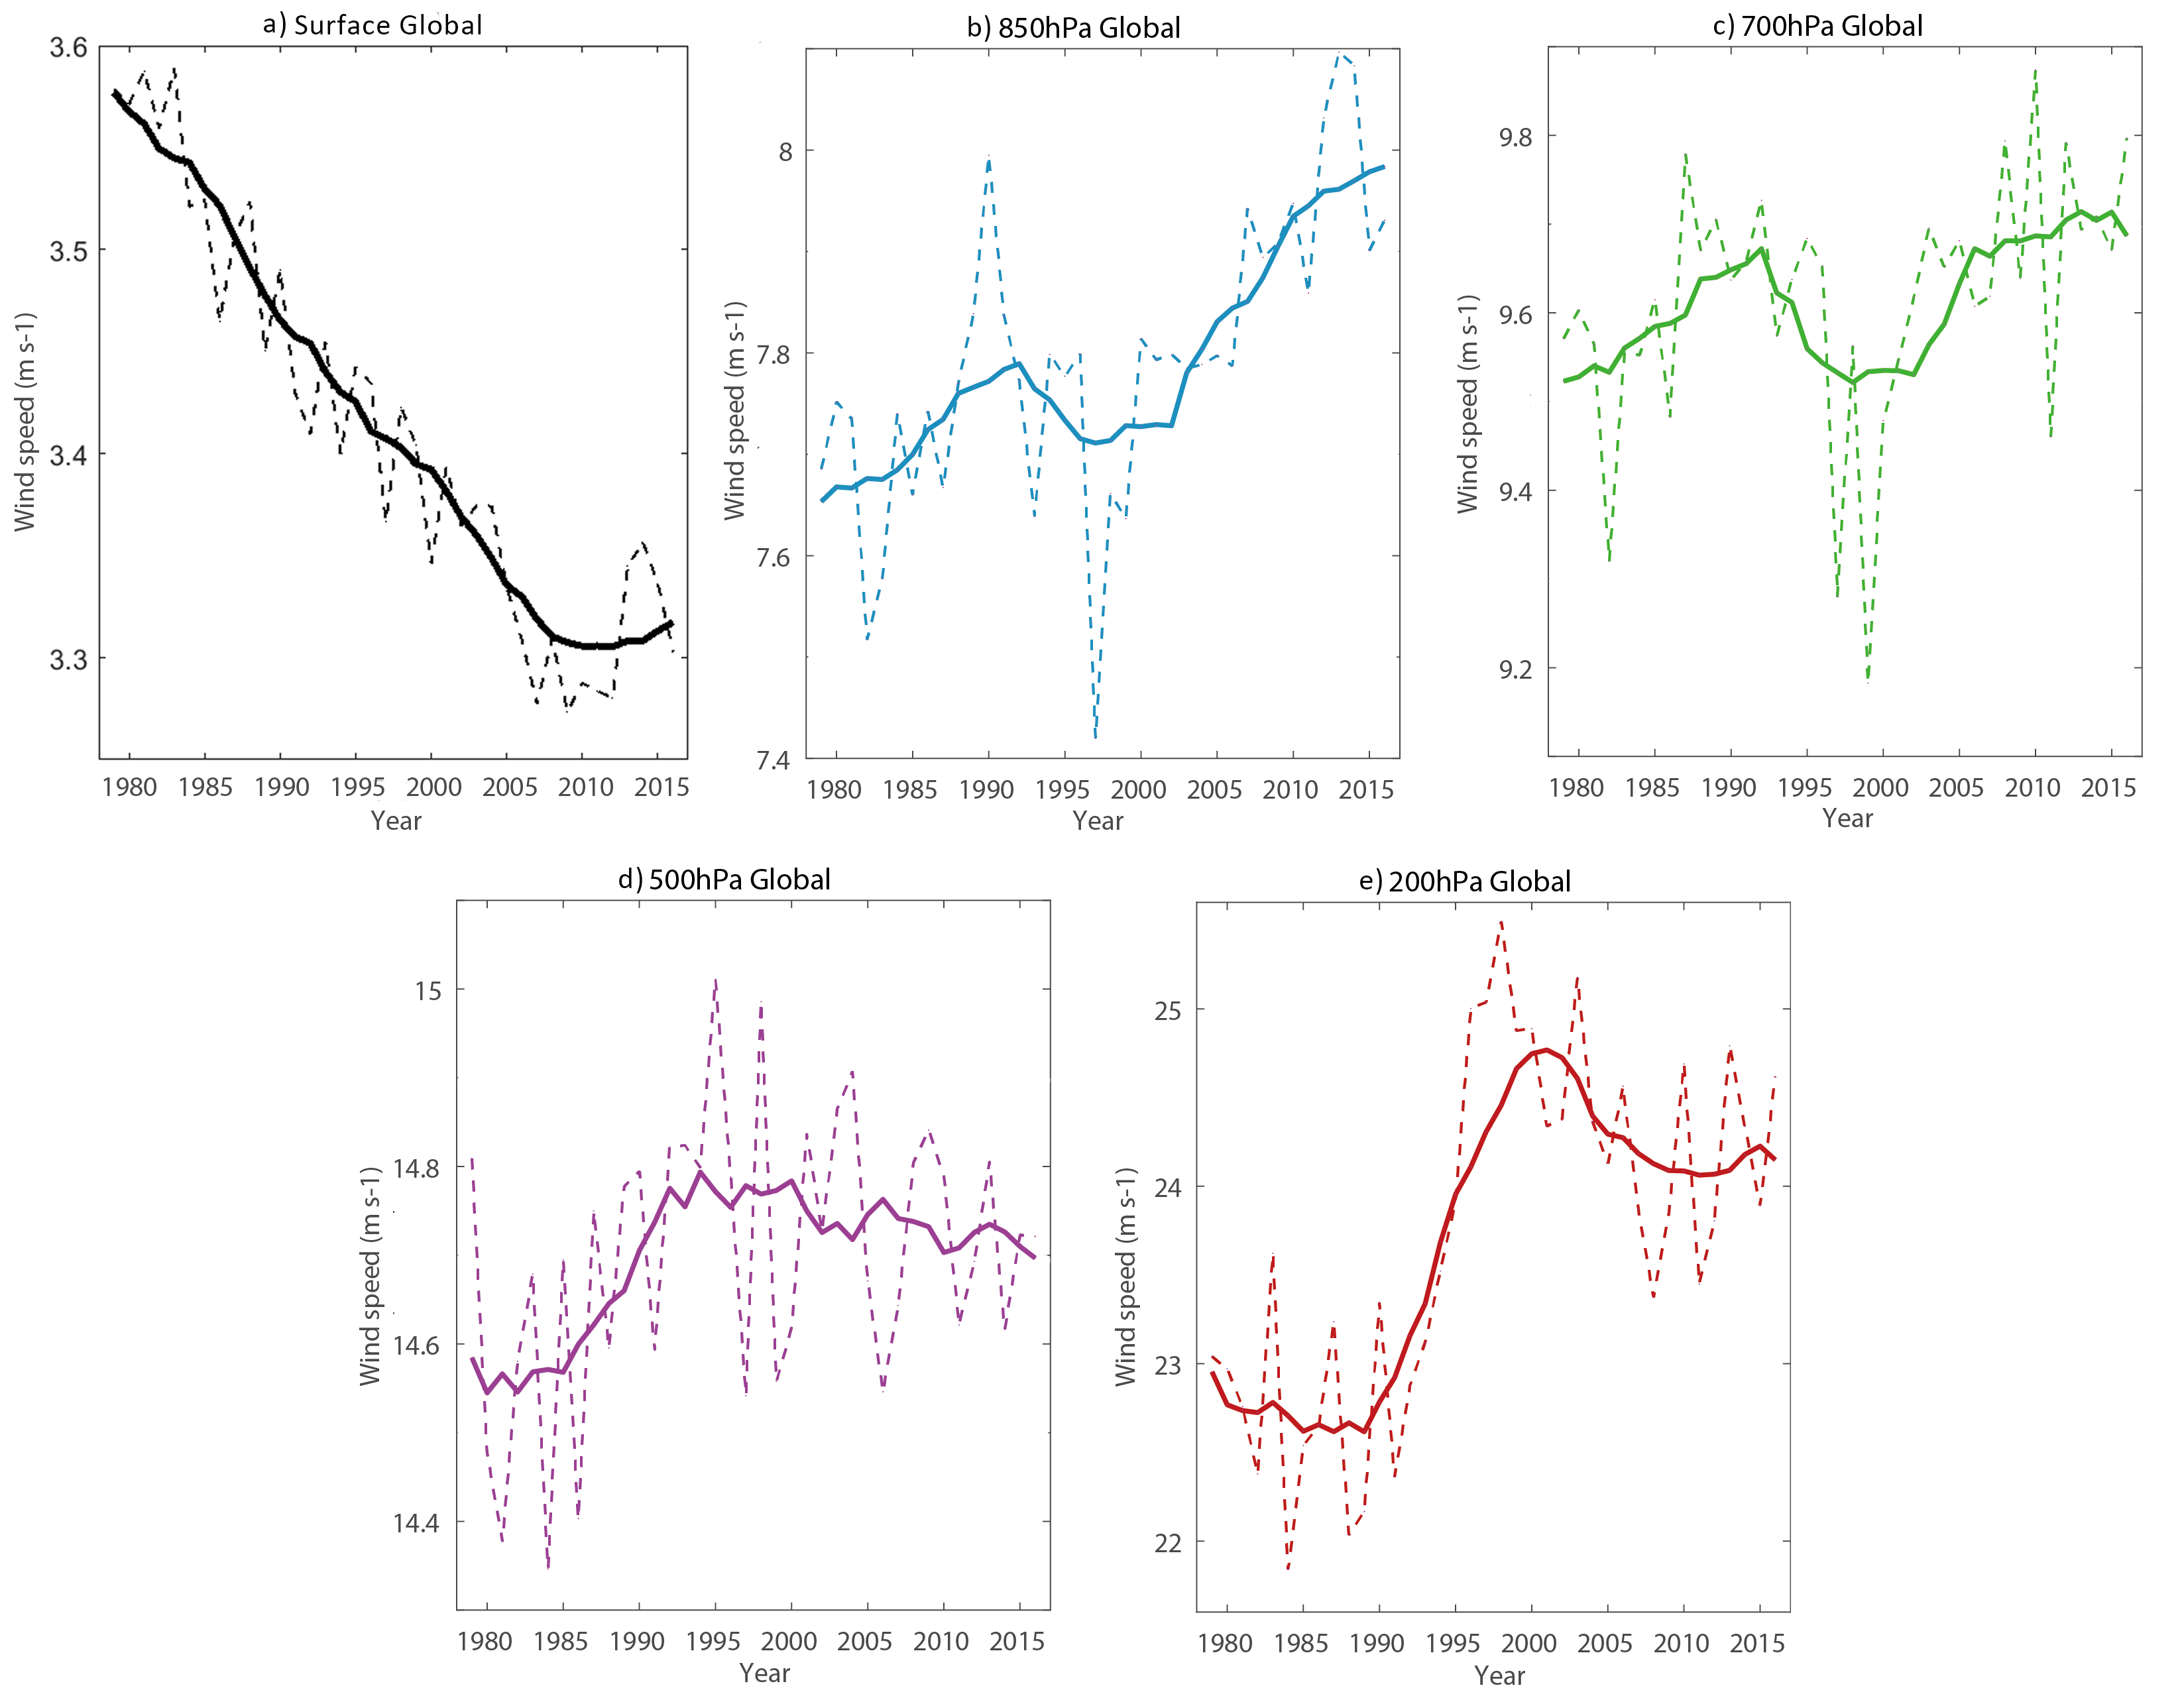
\includegraphics[width=0.85\textwidth]{全球对流层中位数风速演变}
    \bicaption{全球对流层中位数风速演变($m ~ s^{-1}$)。a)地面,b)850 hPa,c)700 hPa,d)500 hPa,e)200 hPa。虚线为各年对应值,实线为虚线9点平滑的结果。}{Global median troposhere wind speed evolution (in $m ~ s^{-1}$). a)Surface, b)850 hPa, c)700 hPa, d)500 hPa, e)200 hPa. Dash line denotes values for every year, solid line is 9-point moving mean of dash line.}
    \label{fig:globaltroposhereevolution}
\end{figure}

\begin{figure}[!t]
    \centering
    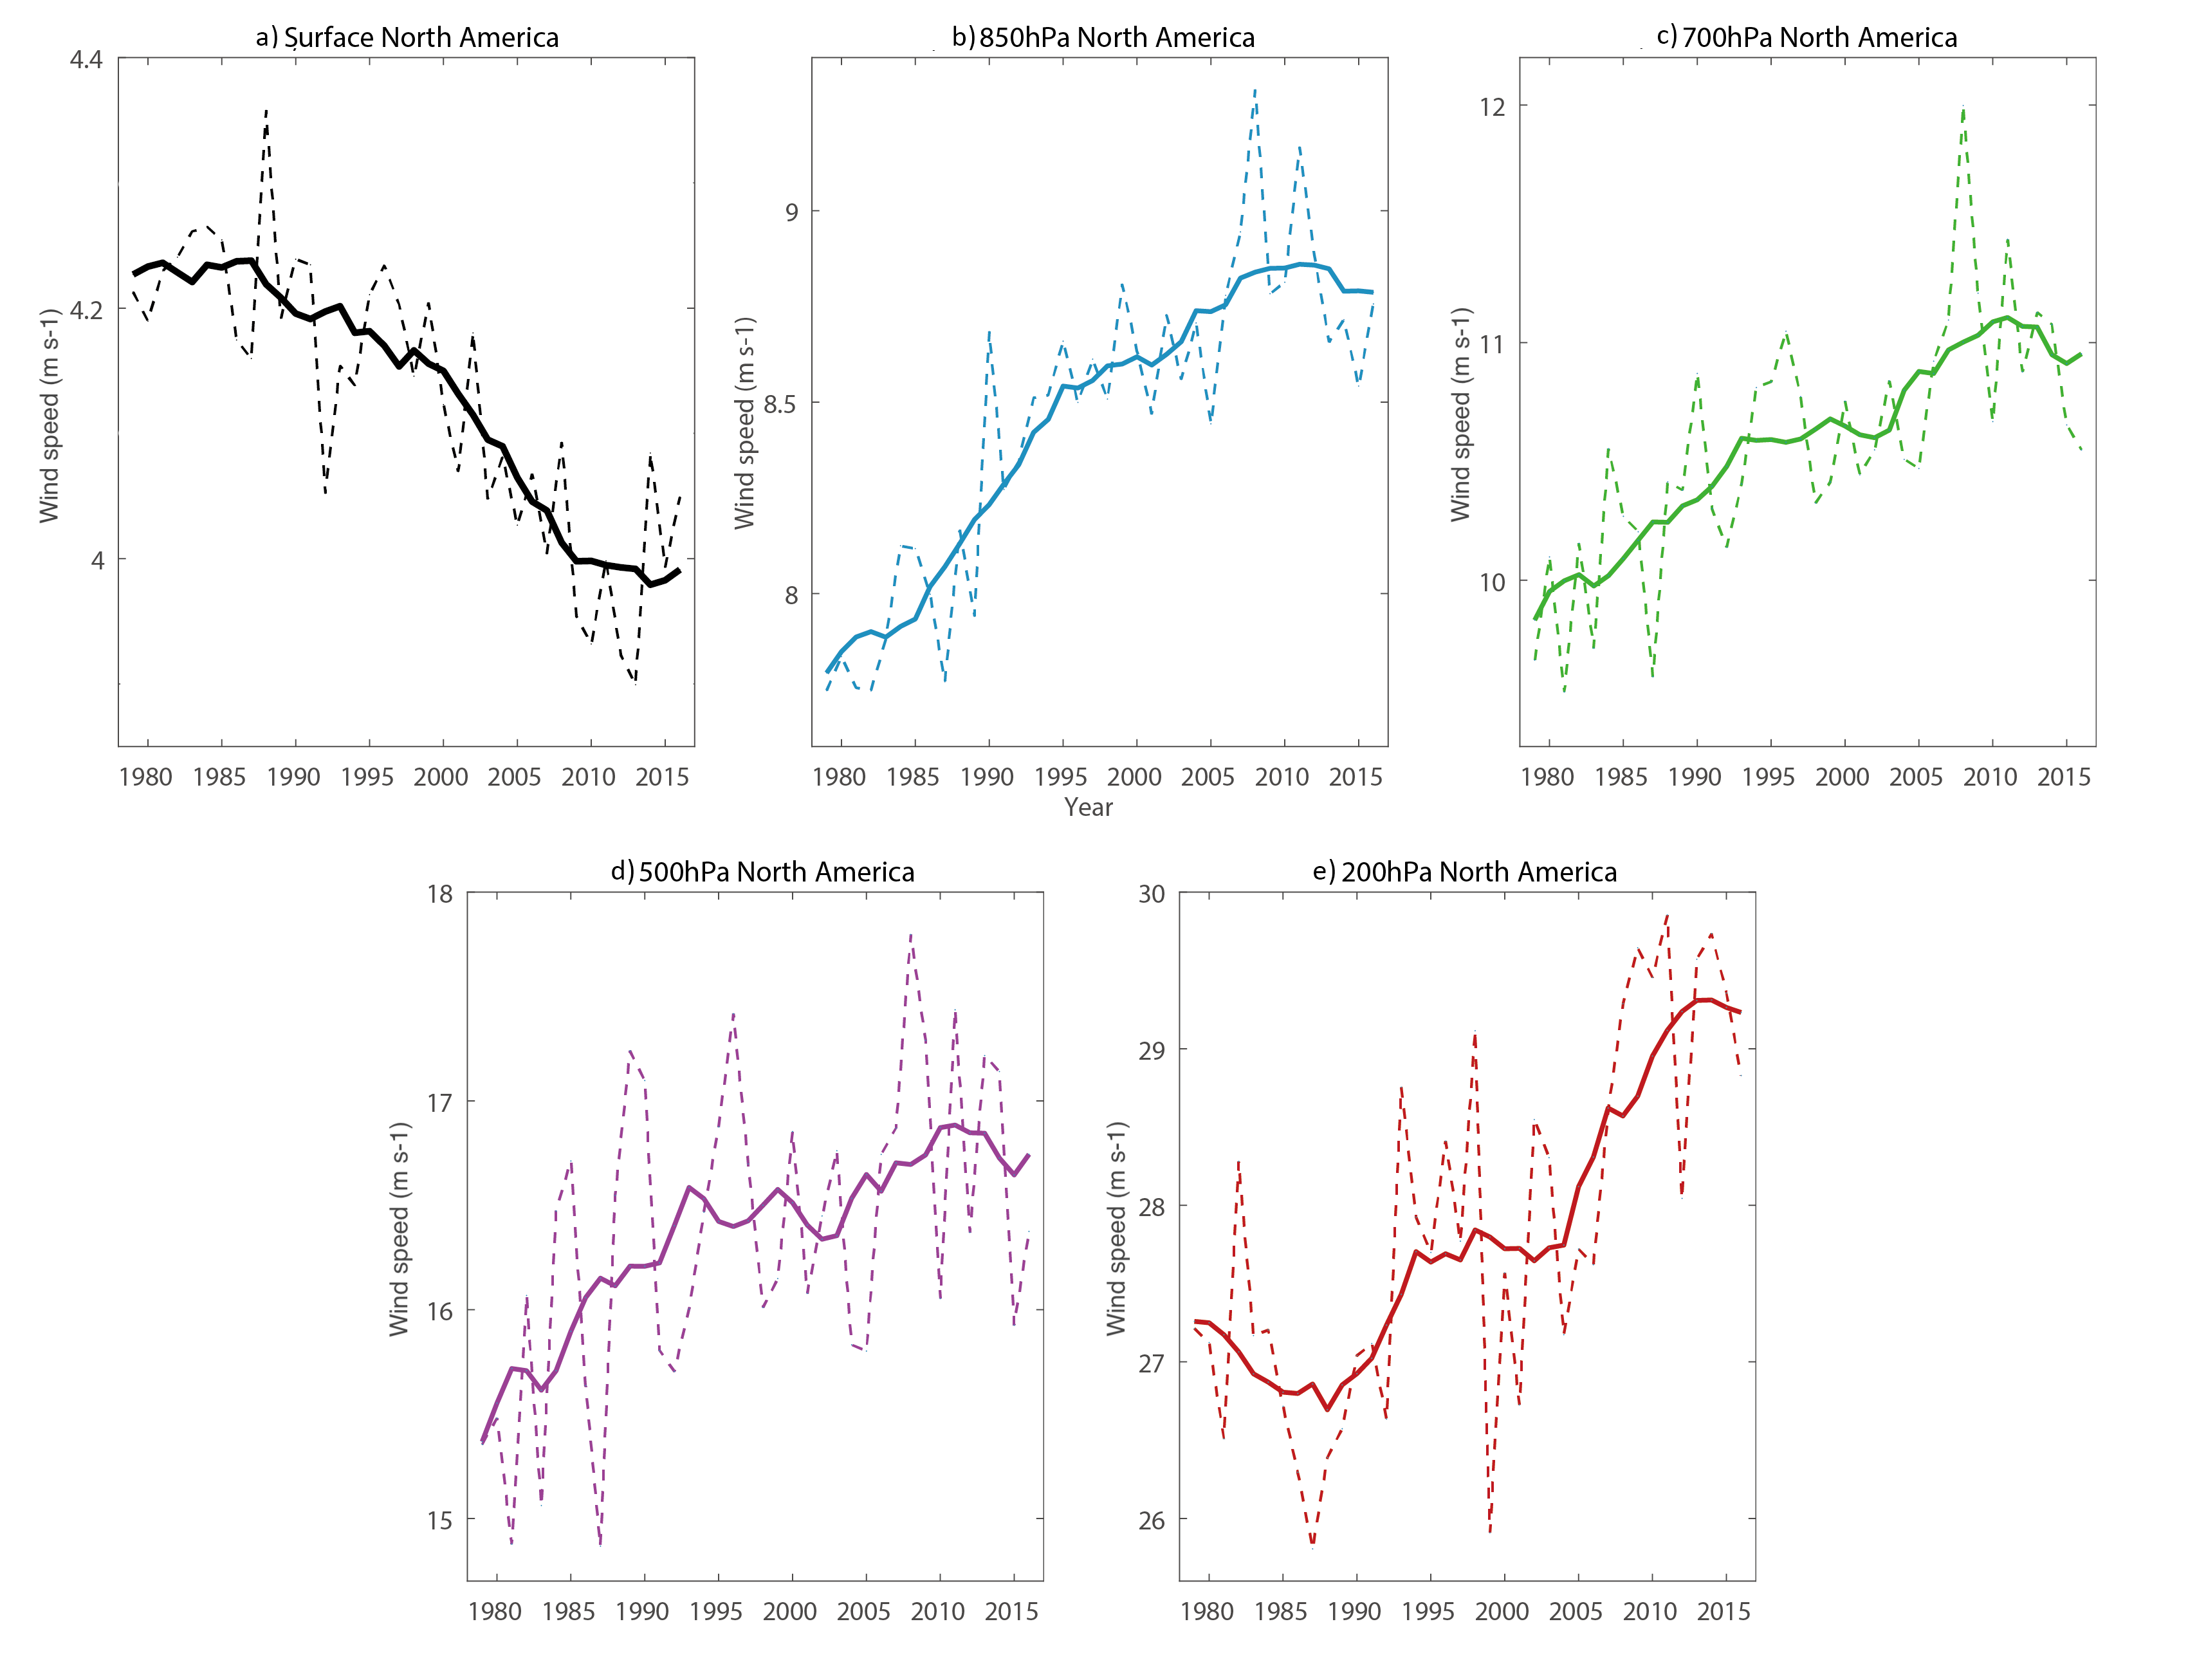
\includegraphics[width=0.85\textwidth]{北美对流层中位数风速演变}
    \bicaption{北美洲对流层中位数风速演变($m ~ s^{-1}$)。与图 \ref{fig:globaltroposhereevolution}类似。}{North American median troposhere wind speed evolution (in $m ~ s^{-1}$). Same as \ref{fig:globaltroposhereevolution}, but for North America.}
    \label{fig:NAtroposhereevolution}
\end{figure}

\begin{figure}[!b]
    \centering
    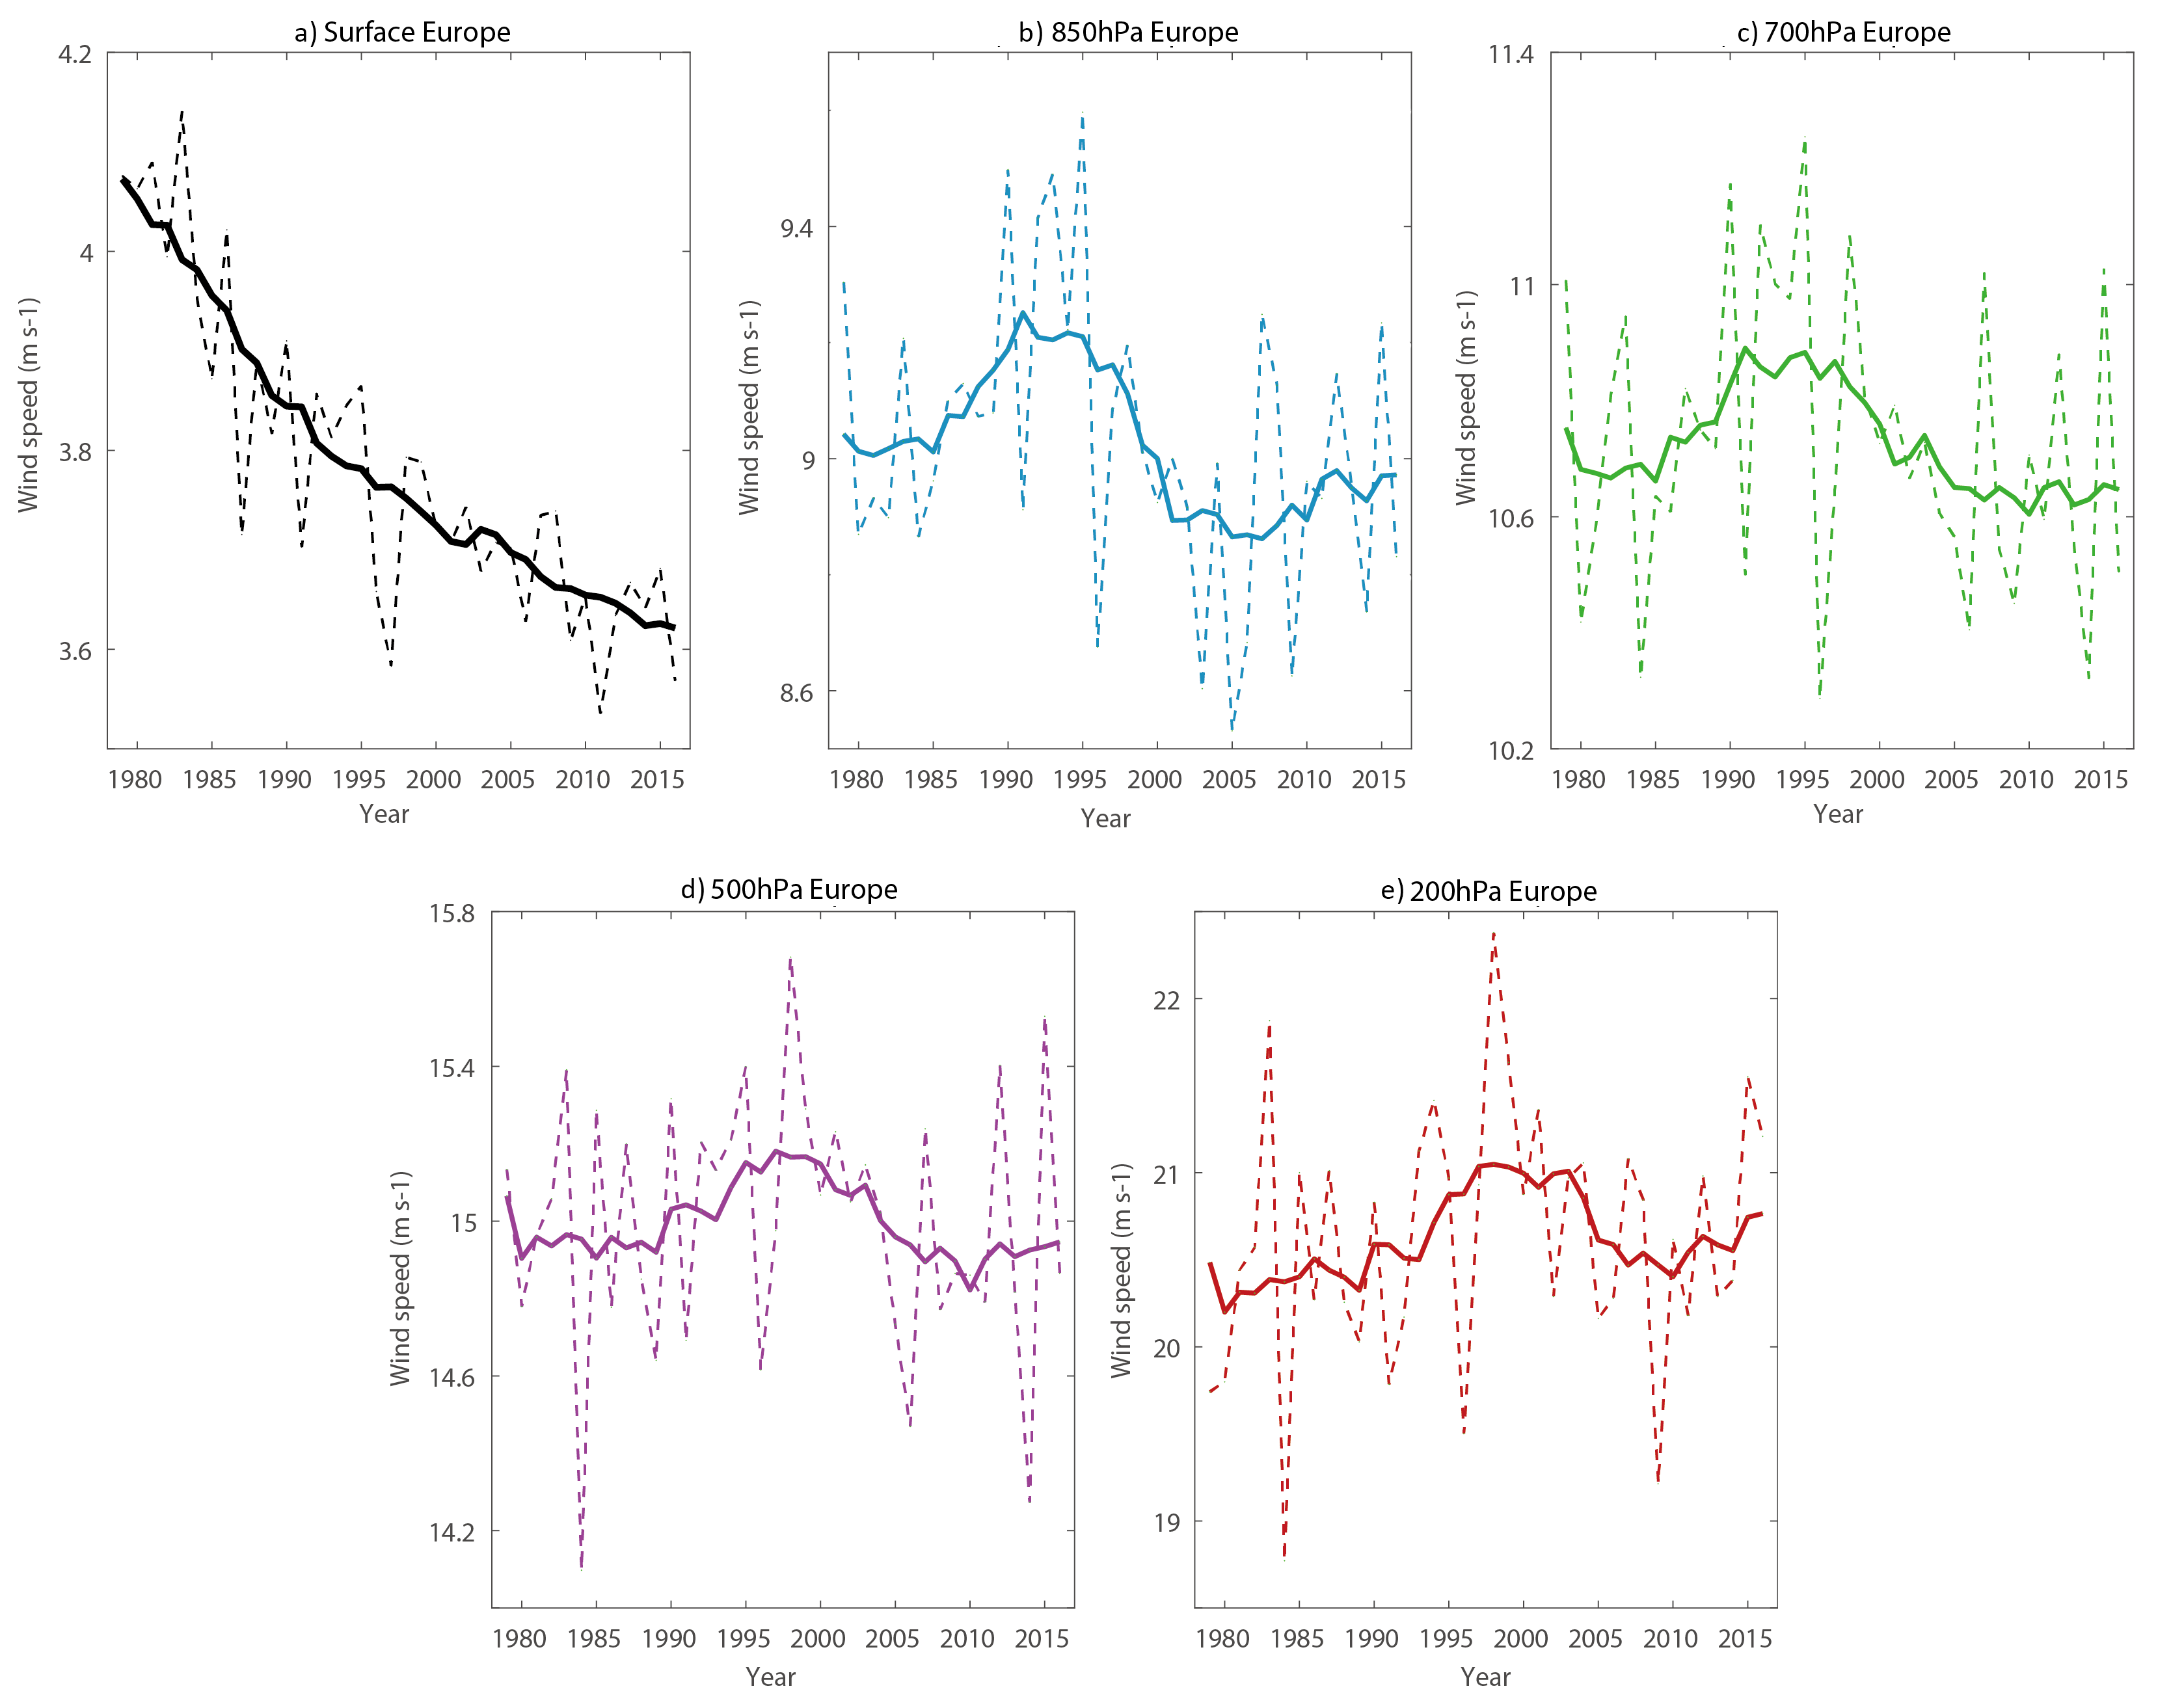
\includegraphics[width=0.85\textwidth]{欧洲对流层中位数风速演变}
    \bicaption{欧洲对流层中位数风速演变($m ~ s^{-1}$)。与图 \ref{fig:globaltroposhereevolution}类似。}{European median troposhere wind speed evolution (in $m ~ s^{-1}$). Same as \ref{fig:globaltroposhereevolution}, but for Europe.}
    \label{fig:EUtroposhereevolution}
\end{figure}

\begin{figure}[!t]
    \centering
    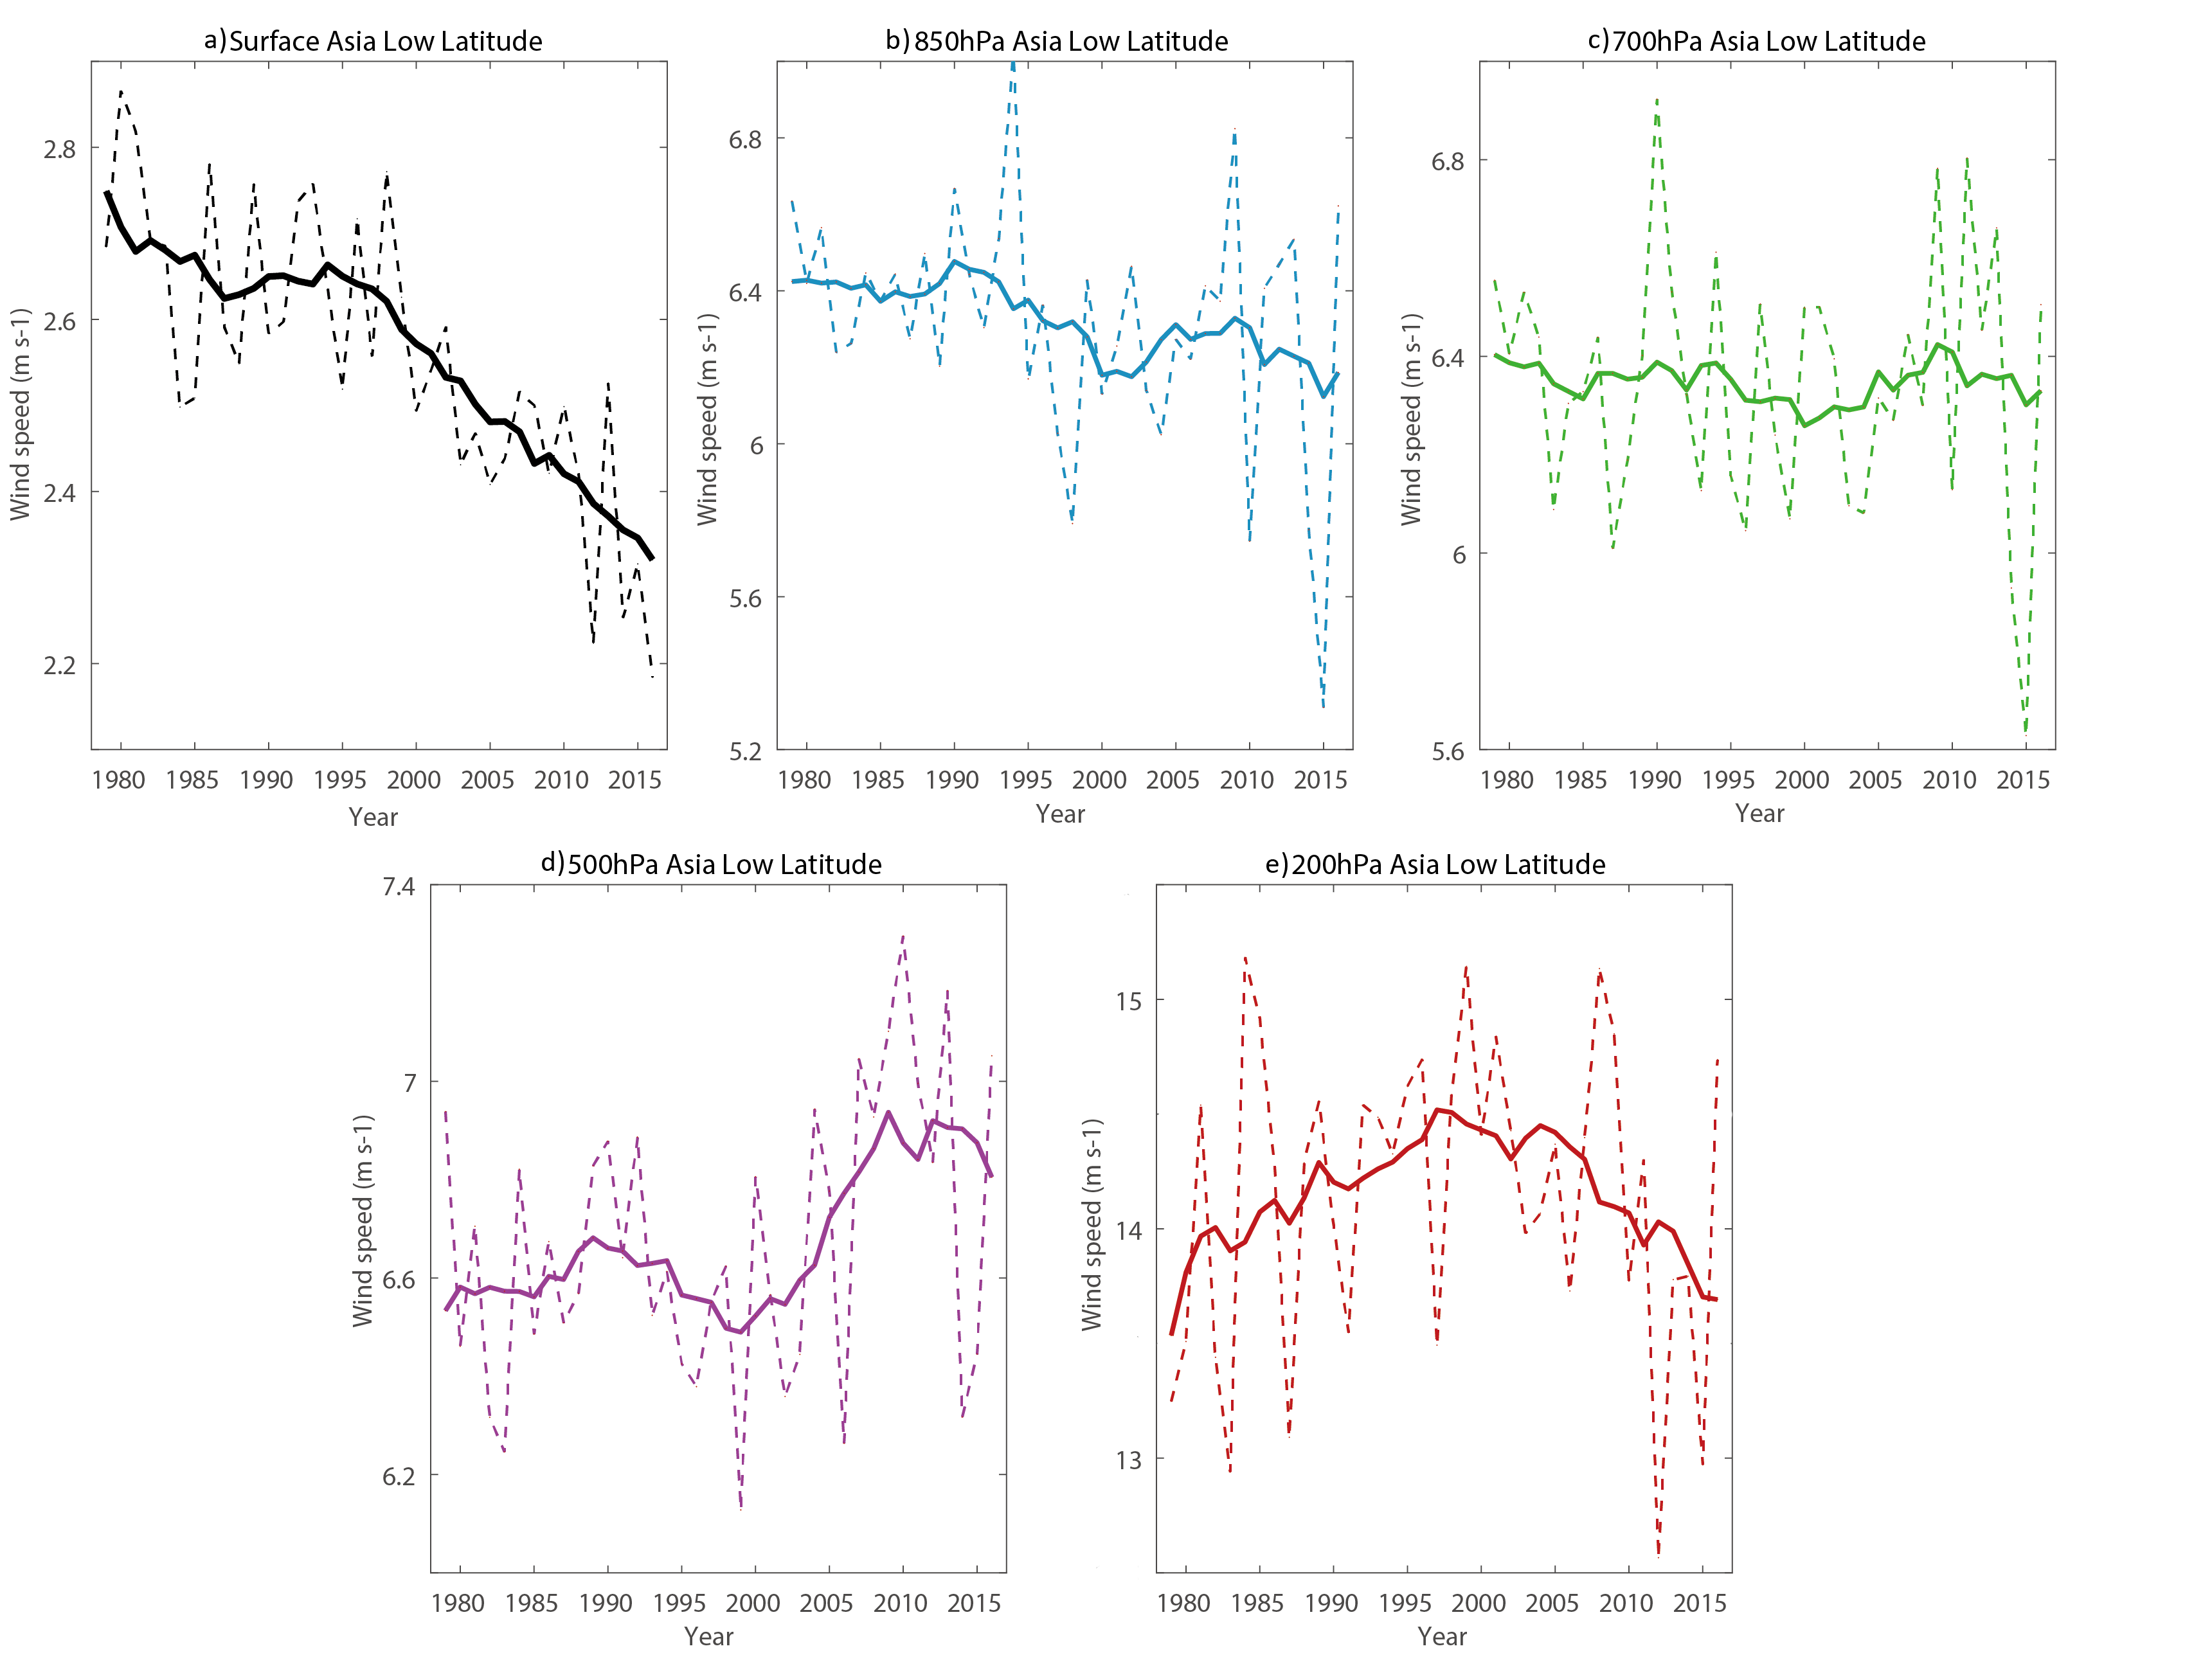
\includegraphics[width=0.85\textwidth]{亚洲低纬度对流层中位数风速演变}
    \bicaption{亚洲低纬度(0 - 20 N)对流层中位数风速演变($m ~ s^{-1}$)。与图 \ref{fig:globaltroposhereevolution}类似。}{Asian low latitude (0 - 20 N) median troposhere wind speed evolution (in $m ~ s^{-1}$). Same as \ref{fig:globaltroposhereevolution}, but for Asia low latitude.}
    \label{fig:ASlowtroposhereevolution}
\end{figure}

\begin{figure}[!b]
    \centering
    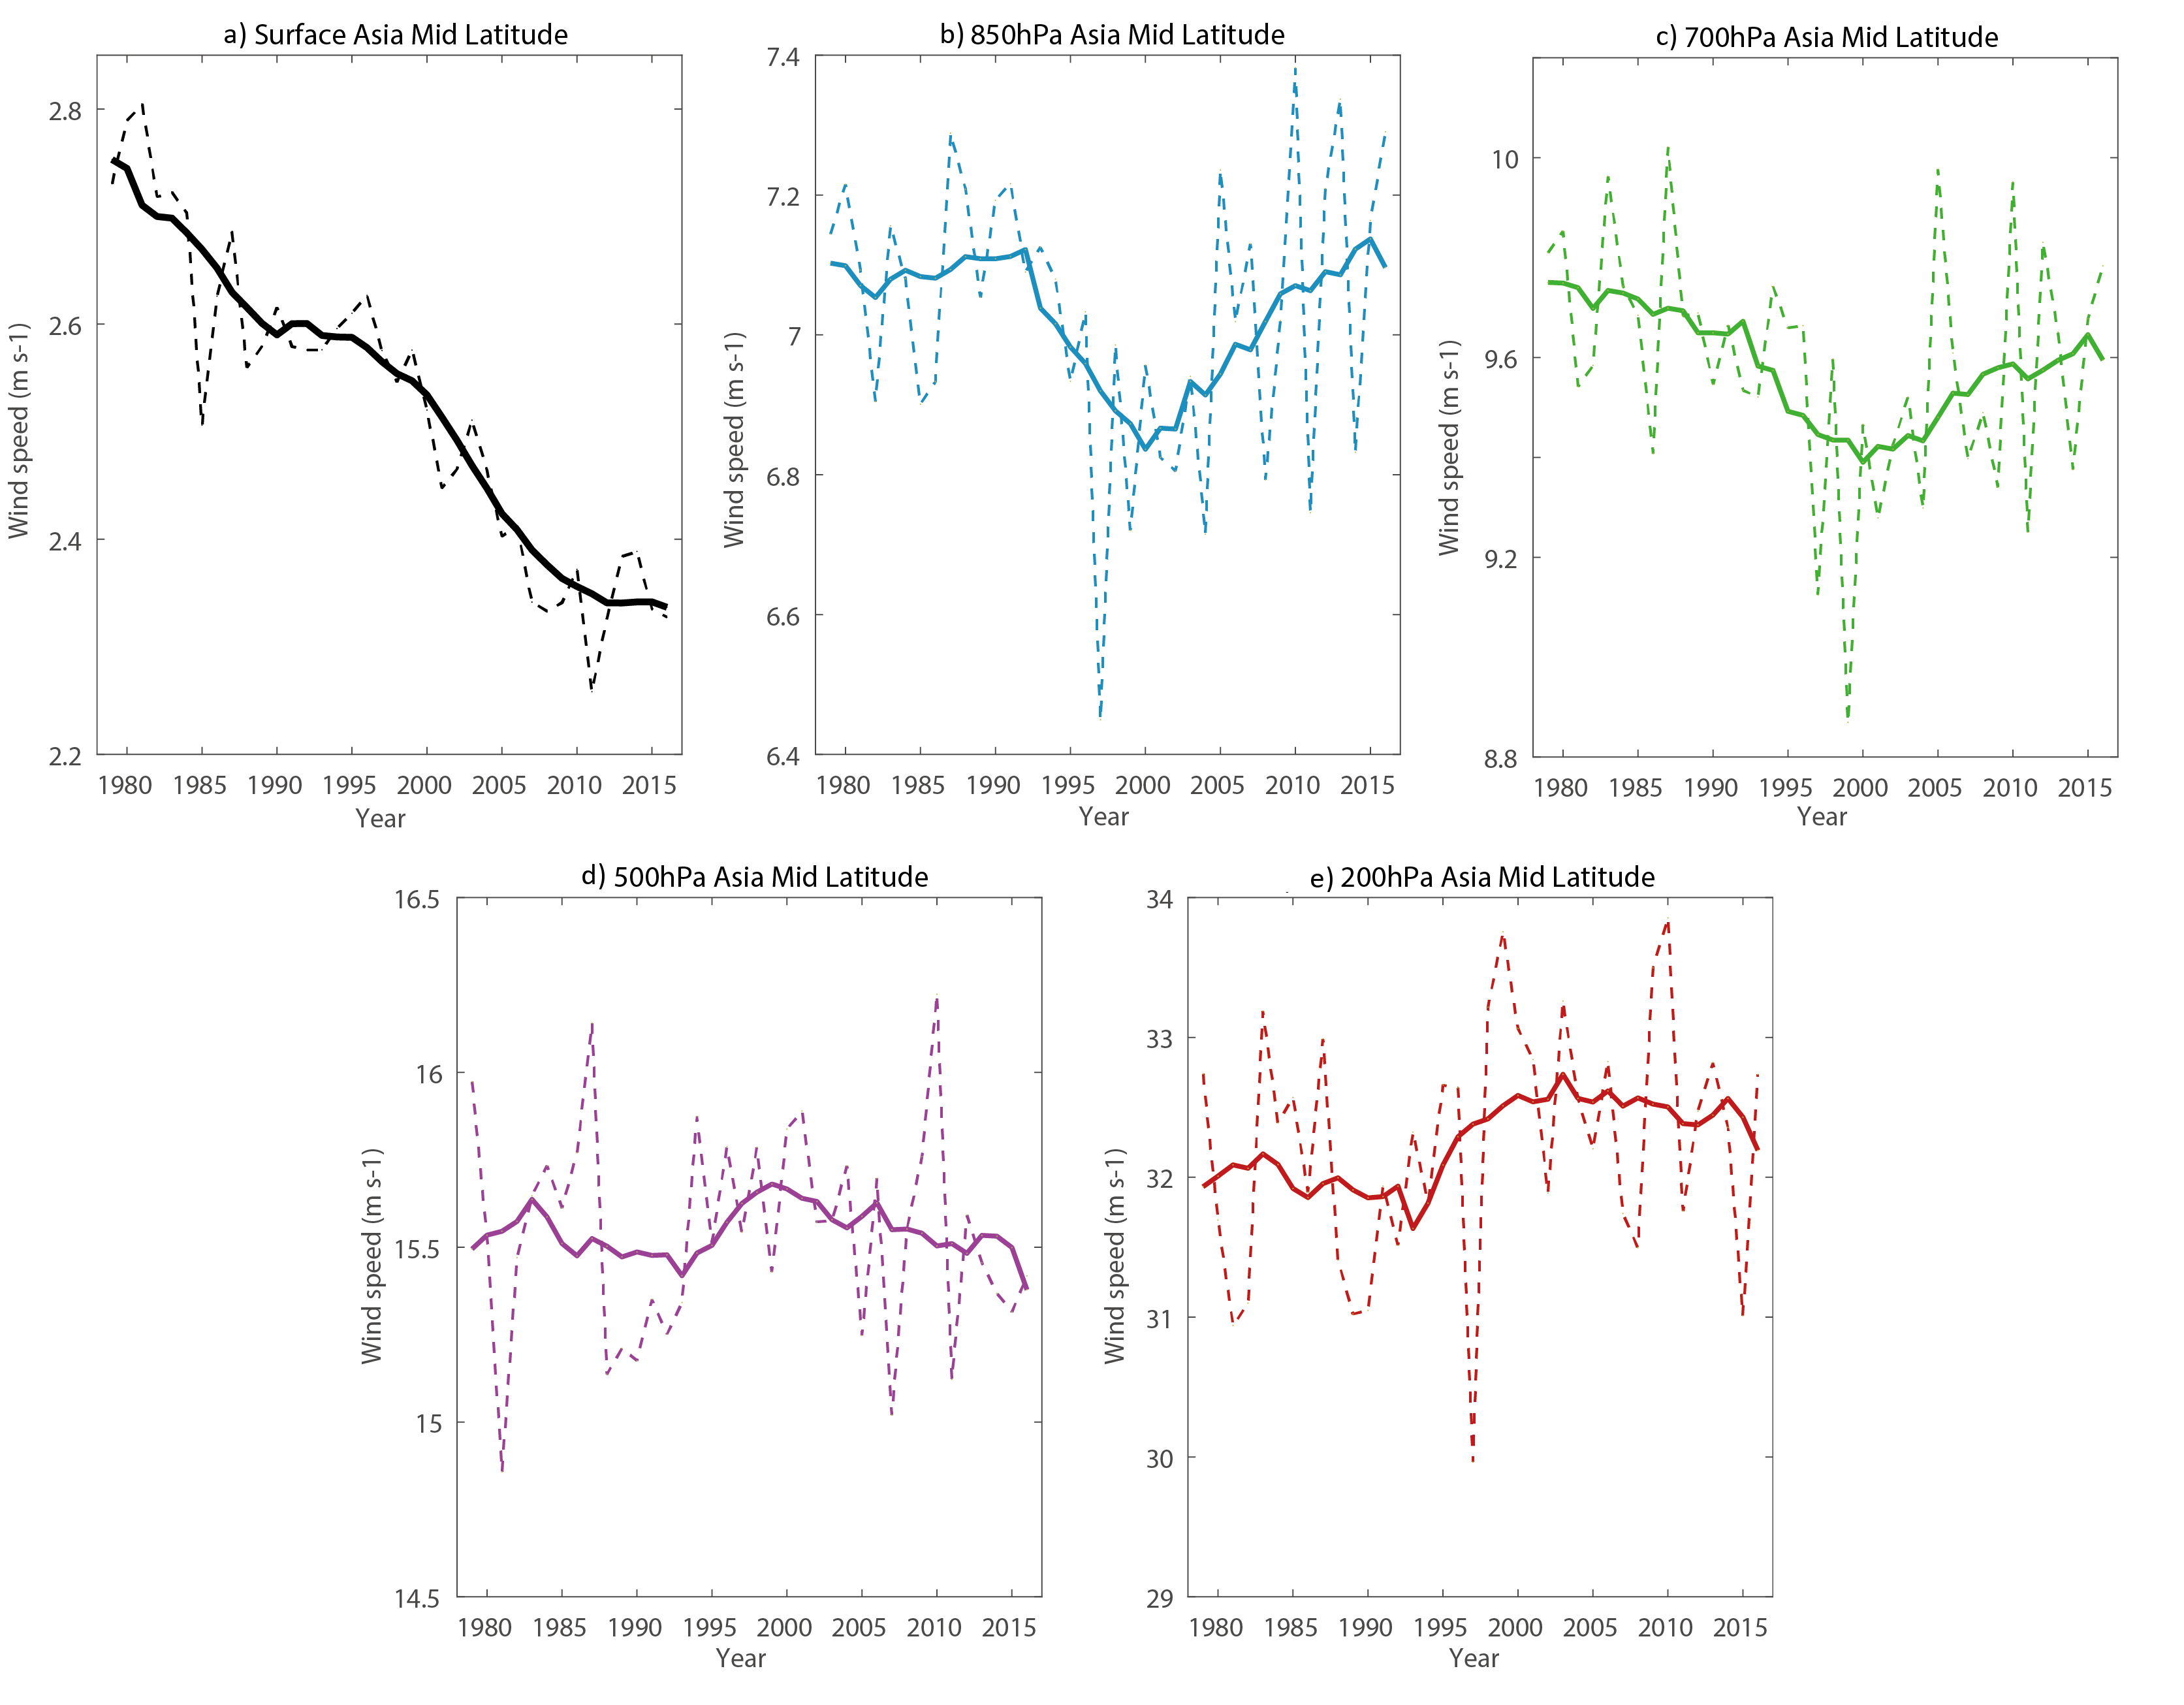
\includegraphics[width=0.85\textwidth]{亚洲中纬度对流层中位数风速演变}
    \bicaption{亚洲中纬度(20 - 55 N)对流层中位数风速演变($m ~ s^{-1}$)。与图 \ref{fig:globaltroposhereevolution}类似。}{Asian mid latitude (20 - 55 N) median troposhere wind speed evolution (in $m ~ s^{-1}$). Same as \ref{fig:globaltroposhereevolution}, but for Asia mid latitude}
    \label{fig:ASmidtroposhereevolution}
\end{figure}

\section{气压场变化的影响}

\begin{figure}[!b]
    \centering
    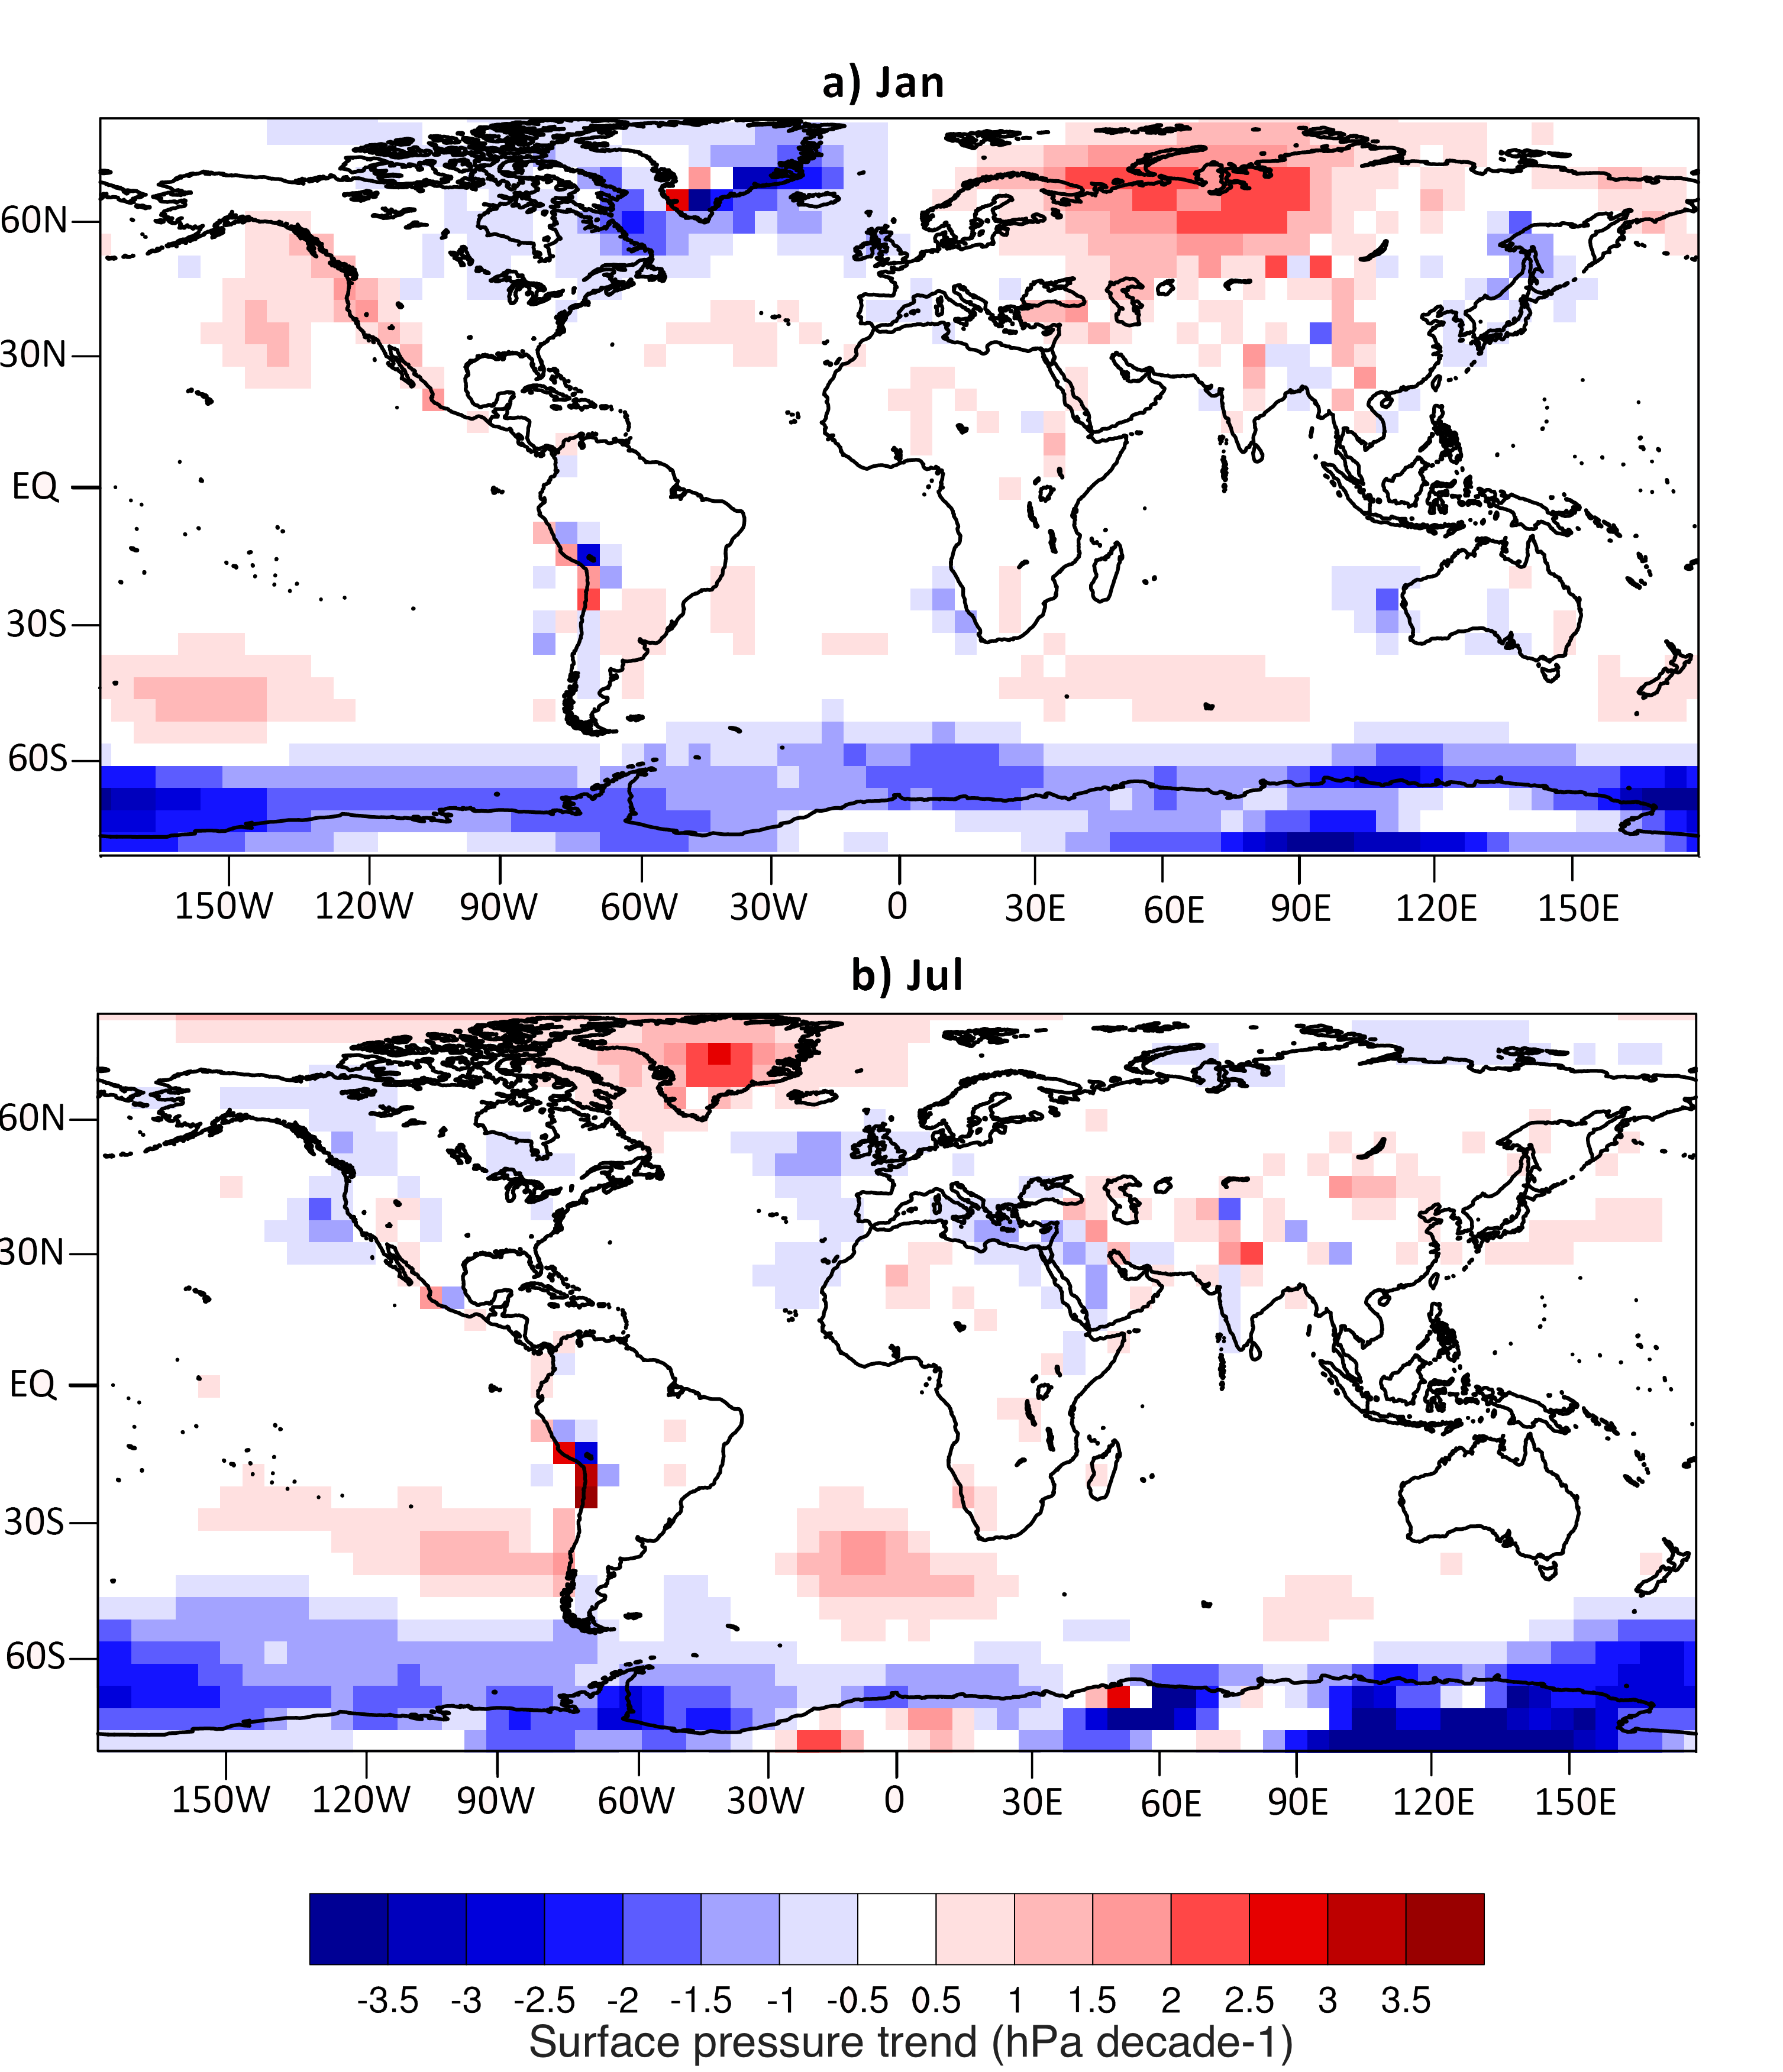
\includegraphics[width=0.8\textwidth]{海平面气压变化}
    \bicaption{海平面气压变化(hPa每十年)。a)一月海平面气压趋势,b)七月海平面气压趋势。}{Change in sea level pressure (in $ hPa ~ decade^{-1}$). a)Trend in January, b)Trend in July. }
    \label{fig:SLPchange}
\end{figure}

1月份海平面气压场的变化主要体现为冰岛低压和西伯利亚高压北部的增强,以及阿留申低压东部的减弱(图 \ref{fig:SLPchange} a))。其中冰岛低压增强会使得北大西洋风暴轴向北偏移,使得欧洲南部风速减小,北部风速增加 \citep{lifland2003the}。而西伯利亚高压北部增强配合日本以北气压下降使得冬季冷空气更容易侵入东亚,这也解释了为何亚洲冬季风速减弱慢于其他季节(第\ref{chap:SpatiotemporalCharacteristics}章 图 \ref{fig:regionalmedianwindtrend})。阿留申低压东南部减弱(即阿留申低压向西北偏移)会使得北太平洋风暴轴向北偏移,造成北美中低纬度风速减小\citep{任雪娟2007北太平洋风暴轴的变异特征及其与中纬度海气耦合关系分析},同时北美风速也会因为冰岛低压增强在北美形成异常偏南气流使得北极冷空气更不容易南下而减小。7月份海平面气压场的变化主要表现为冰岛低压的减弱(图 \ref{fig:SLPchange} b))。冰岛低压的减弱会使得北大西洋风暴轴向南偏移,使得欧洲南部风速增加,北部风速减小。如前文所述,1月份的情况与此刚好相反。这也解释了为何欧洲南部夏季风速减弱明显慢于冬季(第\ref{chap:SpatiotemporalCharacteristics}章 图 \ref{fig:EUwindtrend})。

\section{大尺度海温和环流系统变化的影响}

将北美洲、欧洲、亚洲中纬度和低纬度中位数风速分别与海表温度(SST)做相关,发现它们分别与一些海区SST相关性较高,下面逐个进行分析。

\begin{figure}[!htbp]
    \centering
    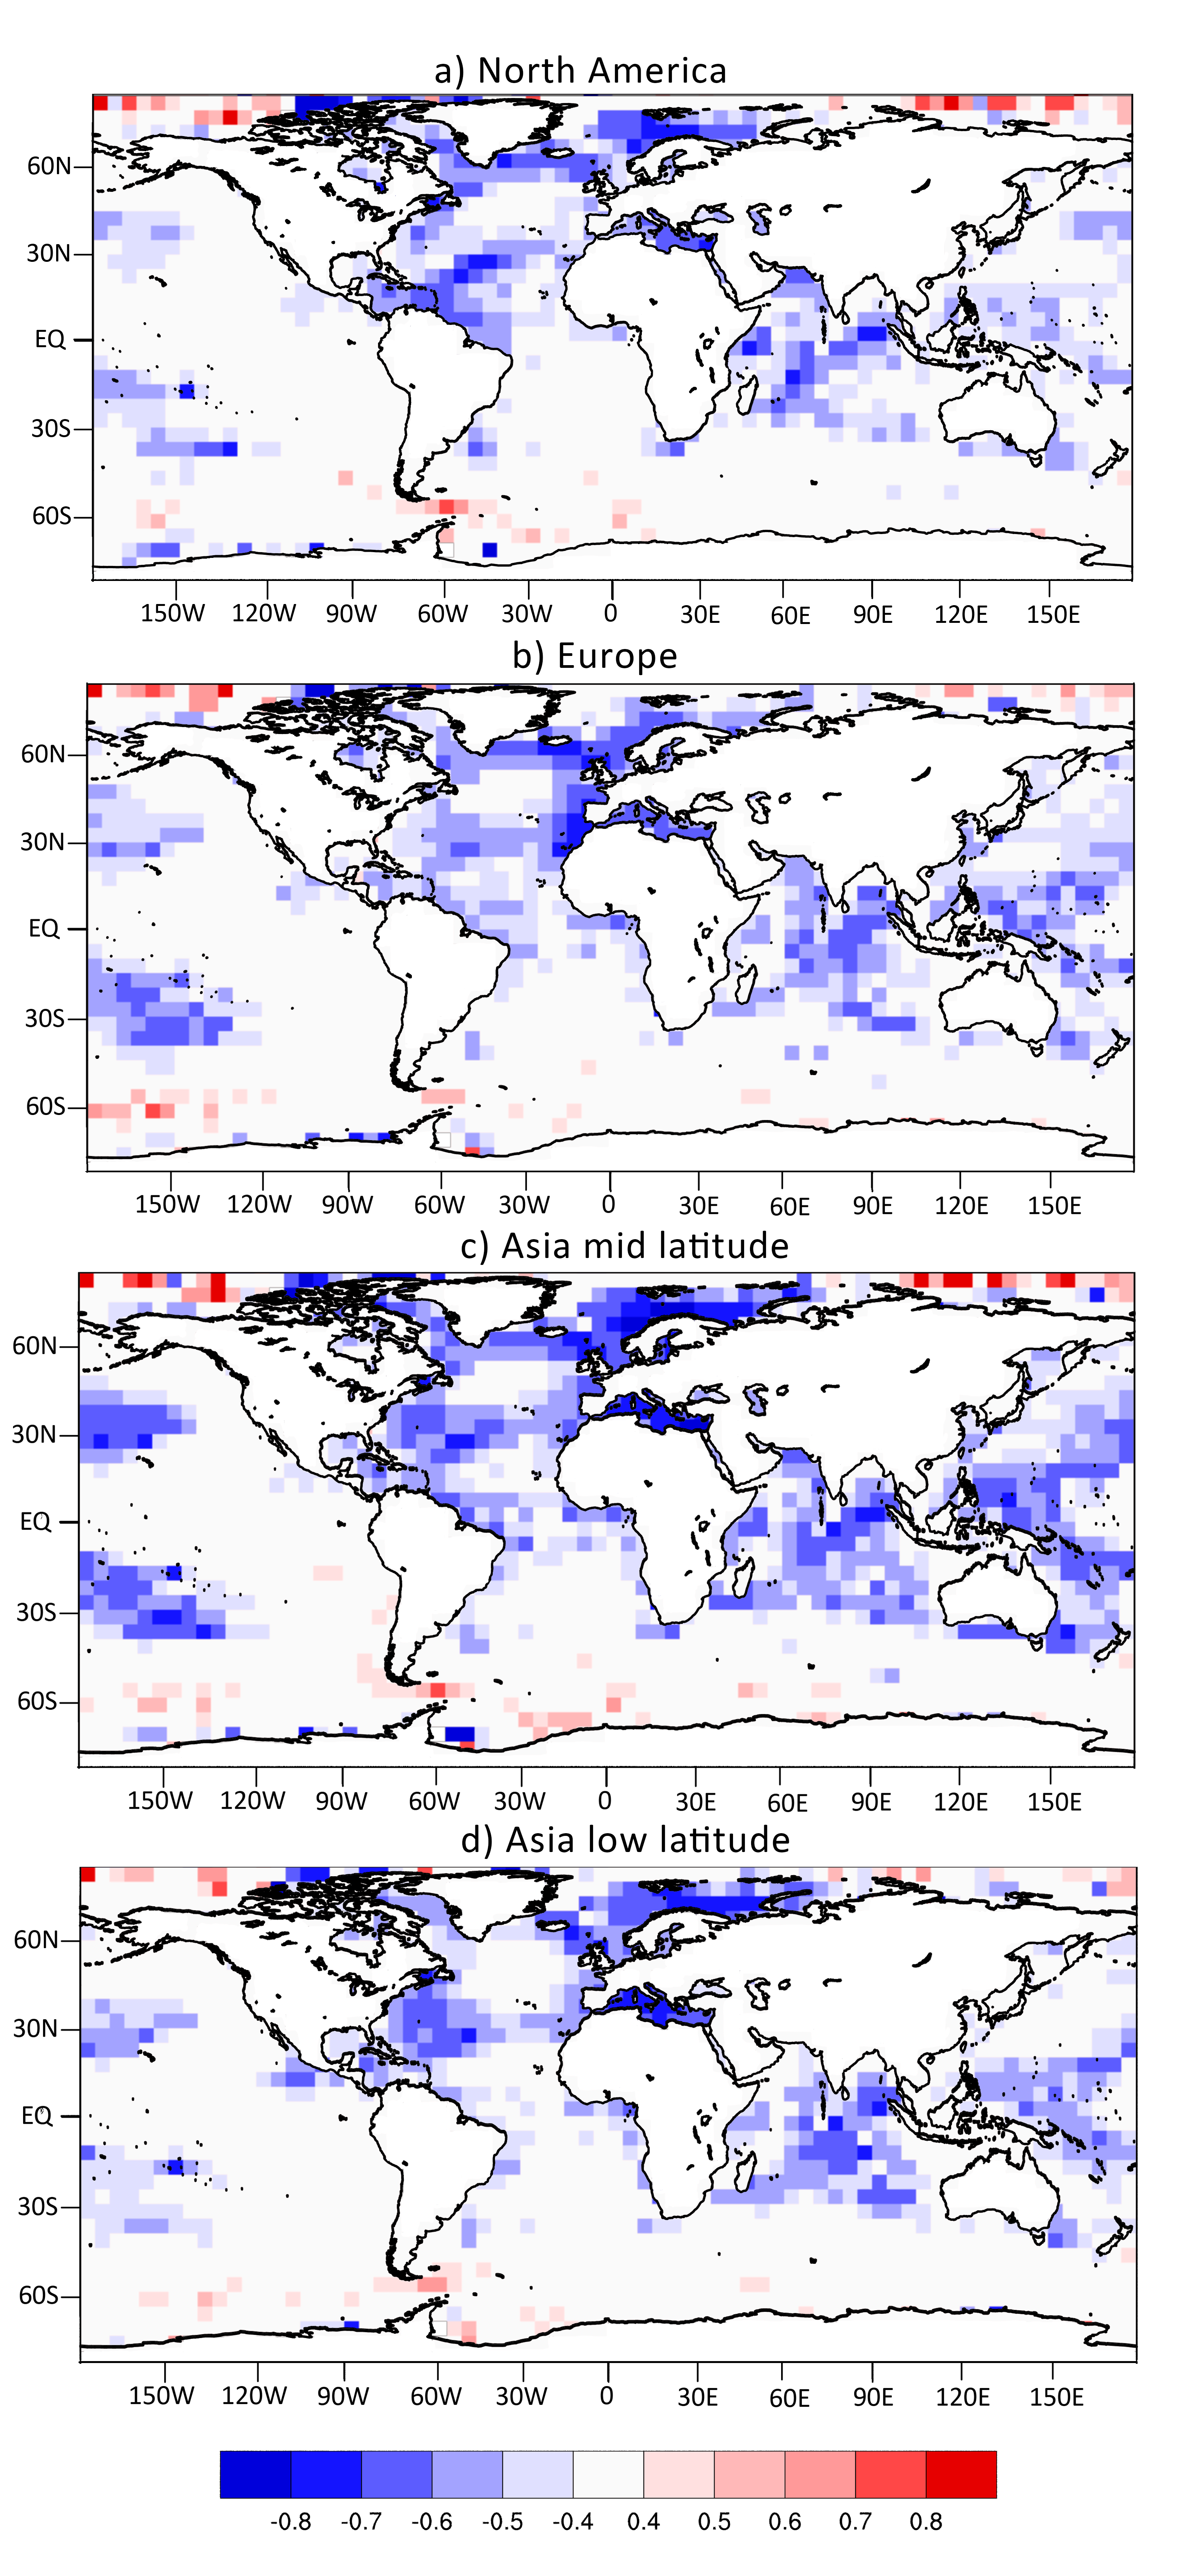
\includegraphics[width=0.63\textwidth]{风速与海温相关系数}
    \bicaption{ 地表风速与海温相关系数。a)北美洲,b)欧洲,c)亚洲中纬度(20 - 55 N)和d)亚洲低纬度(0 - 20 N)中位数风速与海温相关。相关系数0.4对应 p = 0.01}{Correlation coefficient between surface wind speed and SST. Correlation coefficient between median wind speed of a)North America, b)Europe, c)Asia mid latitude (20 - 55 N), d)Asia low latitude (0 - 20 N) and SST. Correlation coefficient of 0.4 corresponds to p = 0.01.}
    \label{fig:windspeedcorrSST}
\end{figure}

北美洲风速与附近的热带北大西洋以及北大西洋高纬海区SST有显著相关关系(图 \ref{fig:windspeedcorrSST} a))。其中,热带北大西洋海温变化可以由热带北大西洋指数(TNA)来表示,对比北美洲中位数风速和TNA的年代际变化,发现二者有相当好的对应关系(r = -0.95, p < 0.01),1987年前二者均较为平稳,1990-2010 北美洲风速持续下降,而TNA指数持续上升,2010年后二者又都回归平稳(图 \ref{fig:NAwindspeedTNA})。有研究表明,TNA正位相会使得中纬度到热带大气低层形成异常的偏北风,此异常风与北美洲中纬度气候态偏南风相反,从而对北美中纬度实际风速产生减弱的效果\citep{wang2002atlantic}。而北美风速与北大西洋高纬海区SST相关则预示着它可能与NAO存在联系。NAO强年冬季北美东部会出现较强的西南气流,阻止北极的冷空气南下,从而使北美东部风速减小。不过这种影响不是非常显著,因而NAO与北美风速没有体现很好的相关关系。

\begin{figure}[!t]
    \centering
    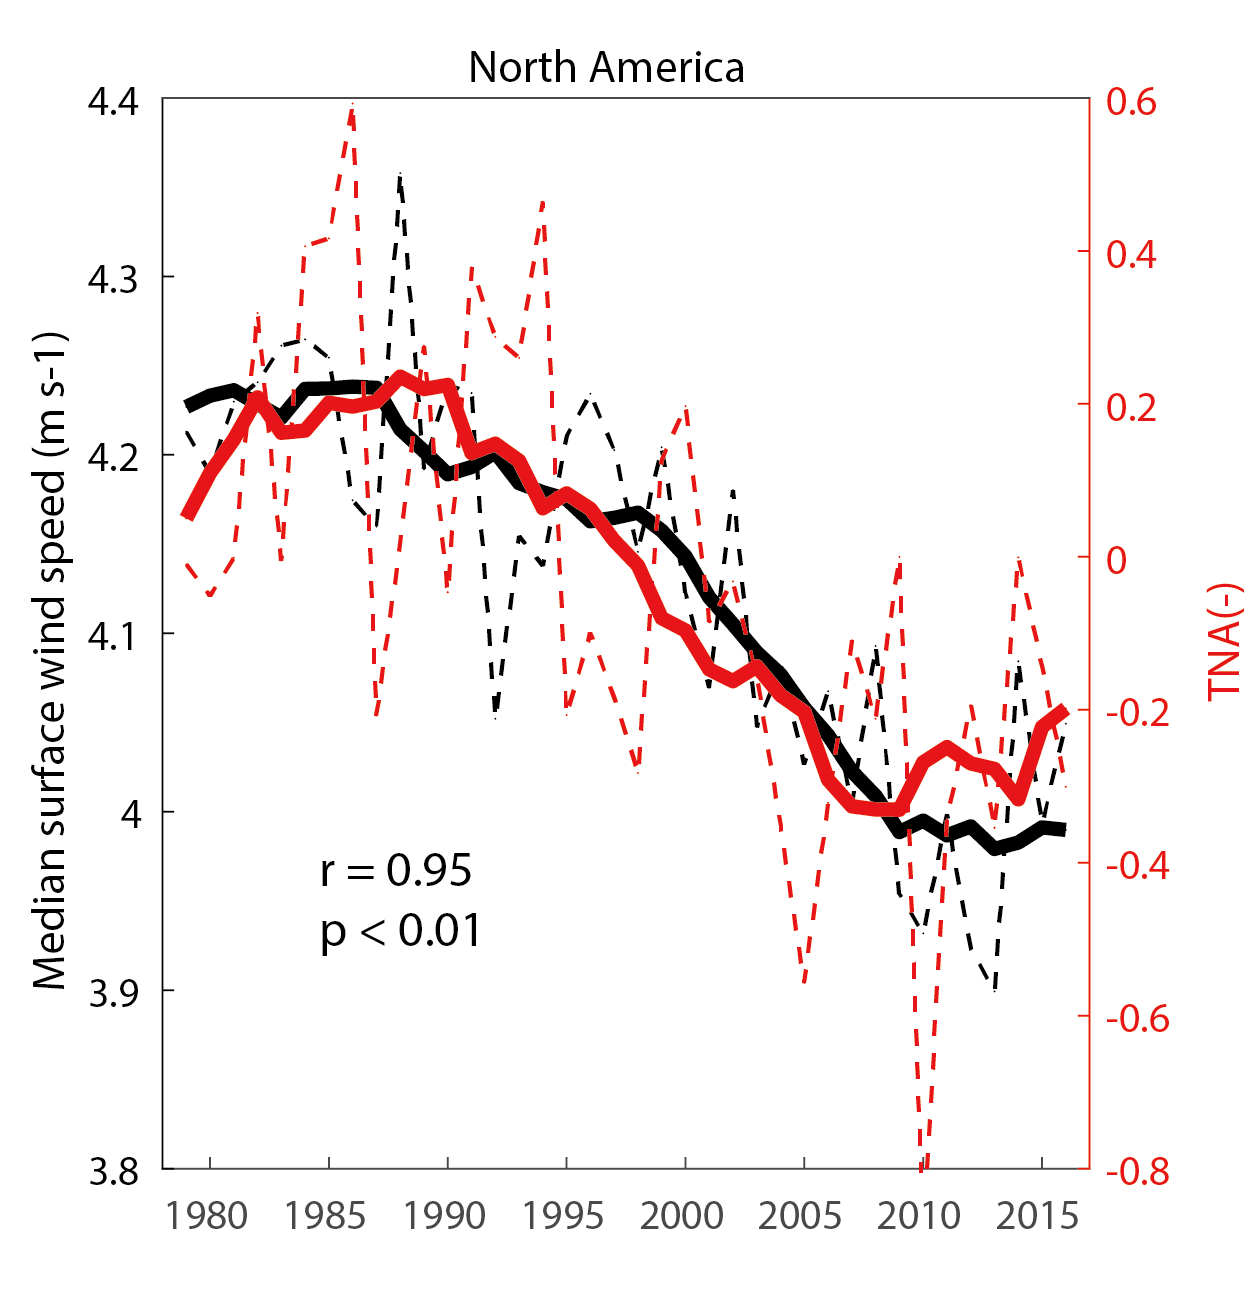
\includegraphics[width=0.45\textwidth]{北美风速与TNA}
    \bicaption{ 北美风速与TNA指数演变。黑色(红色)虚线为北美洲中位数风速(TNA指数年平均值),实线为虚线9年滑动平均结果,两实线的相关系数为0.95,p < 0.01。}{Evolution of North American wind speed and PDO index. Black (red) dash line is North American annual median wind speed (annual mean value of TNA index), solid line is 9-point moving mean of dash line, correlation coefficient between two solid lines is 0.95, p < 0.01.}
    \label{fig:NAwindspeedTNA}
\end{figure}

欧洲风速与北大西洋高纬海温有显著相关,预示着它可能与NAO存在关联(图 \ref{fig:windspeedcorrSST} b))。将去趋势的欧洲中位数风速序列与NAO指数对比发现,二者有显著相关,相关系数达到 -0.48(p < 0.01)(图 \ref{fig:EUwindspeedNAO})。之前已有许多研究发现NAO与欧洲风速的相关关系\citep{beniston2005mountain, earl20131980–2010, zeng2019a}。目前普遍认为,NAO对欧洲风速的影响通过以下过程进行:NAO的强弱会影响北大西洋上空急流的位置,而急流位置的改变又会使风暴轴发生偏移,当NAO处于正位相是,风暴轴偏北,使得气旋在欧洲活动的位置偏北,最终造成欧洲南部风速偏小,而北部偏大,NAO处于负位相时刚好相反\citep{lifland2003the, zeng2019a}。由于研究所用到的站点位于欧洲北部的较少,所以NAO对于欧洲南部的影响会主导分析的结果。

\begin{figure}[!b]
    \centering
    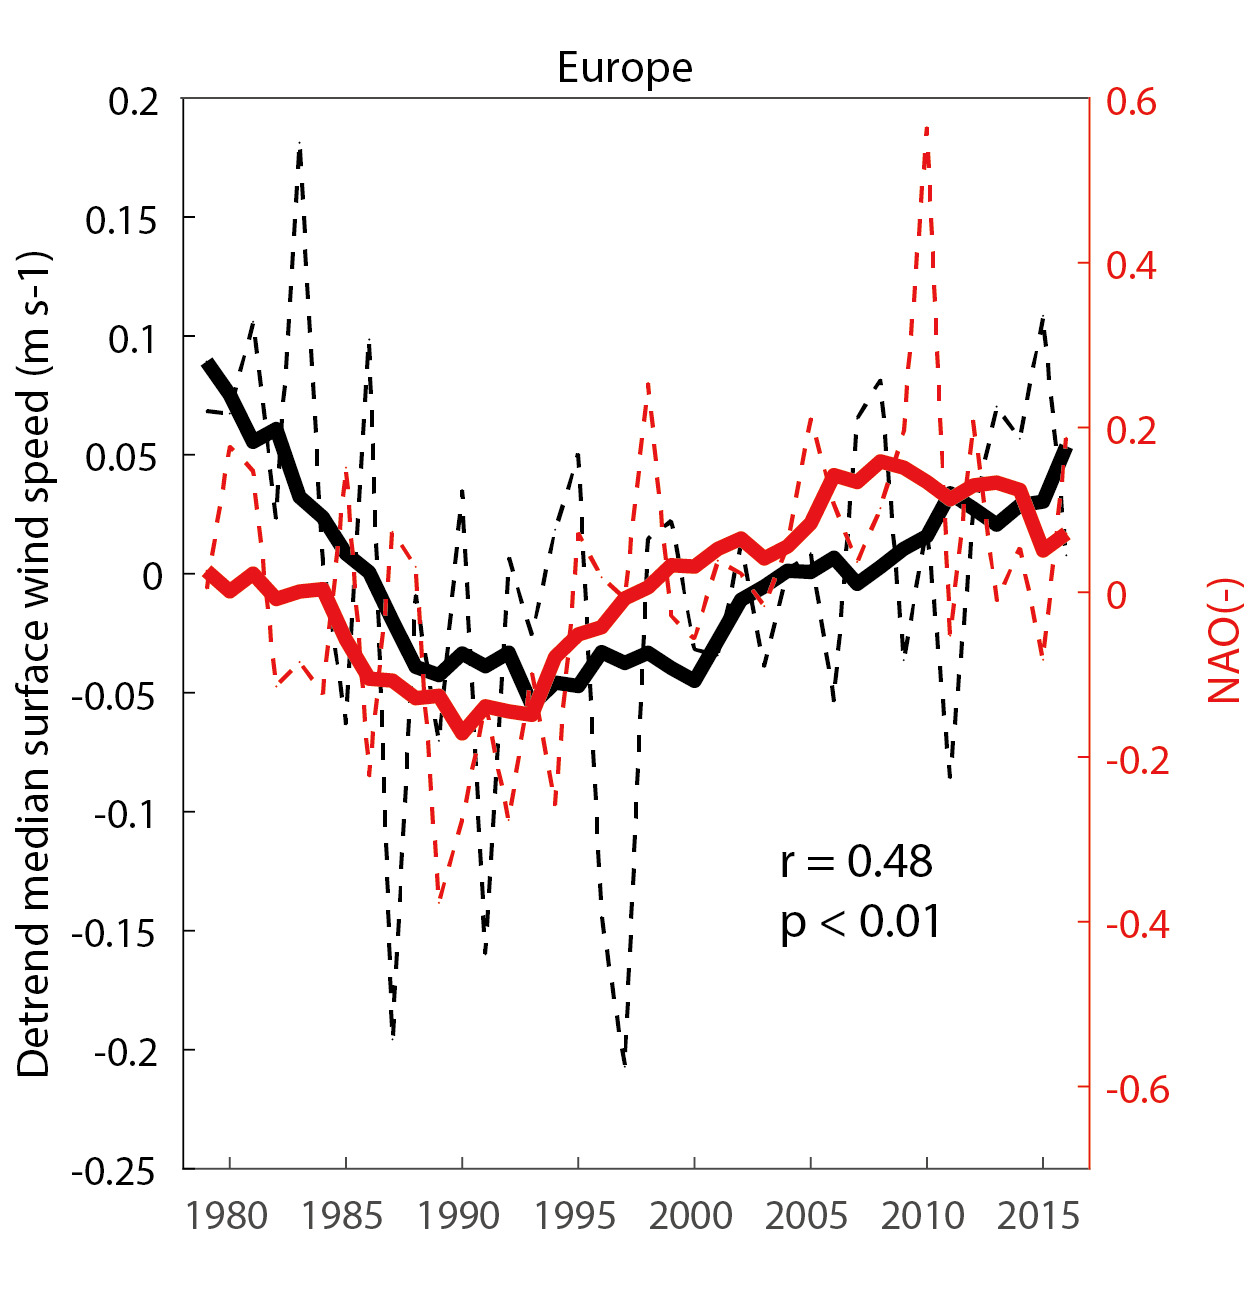
\includegraphics[width=0.45\textwidth]{欧洲风速与NAO}
    \bicaption{ 欧洲风速与NAO指数演变。黑色(红色)虚线为欧洲中位数风速(NAO指数年平均值),实线为虚线9年滑动平均结果,两实线的相关系数为0.48,p < 0.01。}{Evolution of European wind speed and NAO index. Black (red) dash line is European annual median wind speed (annual mean value of NAO index), solid line is 9-point moving mean of dash line, correlation coefficient between two solid lines is 0.48, p < 0.01.}
    \label{fig:EUwindspeedNAO}
\end{figure}

亚洲低纬度风速与印度洋海温有较强的相关(图 \ref{fig:windspeedcorrSST} d))。\citet{yang2010linking}发现,印度洋偶极子模态(IOB)会使得印度冬季风减弱,从使亚洲低纬度陆地地表风速减小。近期有许多研究表明,南亚季风出现了减弱的现象\citep{bollasina2011anthropogenic, sooraj2015global},印度洋海温变化或许在其中起到了一定作用。

亚洲中纬度风速与中纬度北太平洋、中纬度南太平洋和西太平洋以及印度洋海温有较强相关(图 \ref{fig:windspeedcorrSST} c))。其中它与中纬度北太平和中纬度南太平相关预示着于PDO之间的联系。PDO负位相会产生异常的东风,与中纬度盛行的西风相抵消,从而使亚洲中纬度风速减小\citep{zeng2019a}。此外,西太平洋暖池区也与亚洲中纬度风速有很好的负相关,其中的关联在于夏季西太平洋暖池增温速度快于东亚大陆,海陆热力对比减小从而减弱了东亚夏季风,造成亚洲中纬度风速减小\citep{xu2006steady}。将PDO指数与去趋势的西太平洋暖池面积指数作为回归量回归到去趋势的亚洲中纬度风速序列,发现有一定的相关性(图 \ref{fig:ASwindspeedPDOandWPWPA})。印度洋海温影响亚洲中纬度风速的方式应与其影响亚洲低纬度类似,但影响可能并不显著。

\begin{figure}[!b]
    \centering
    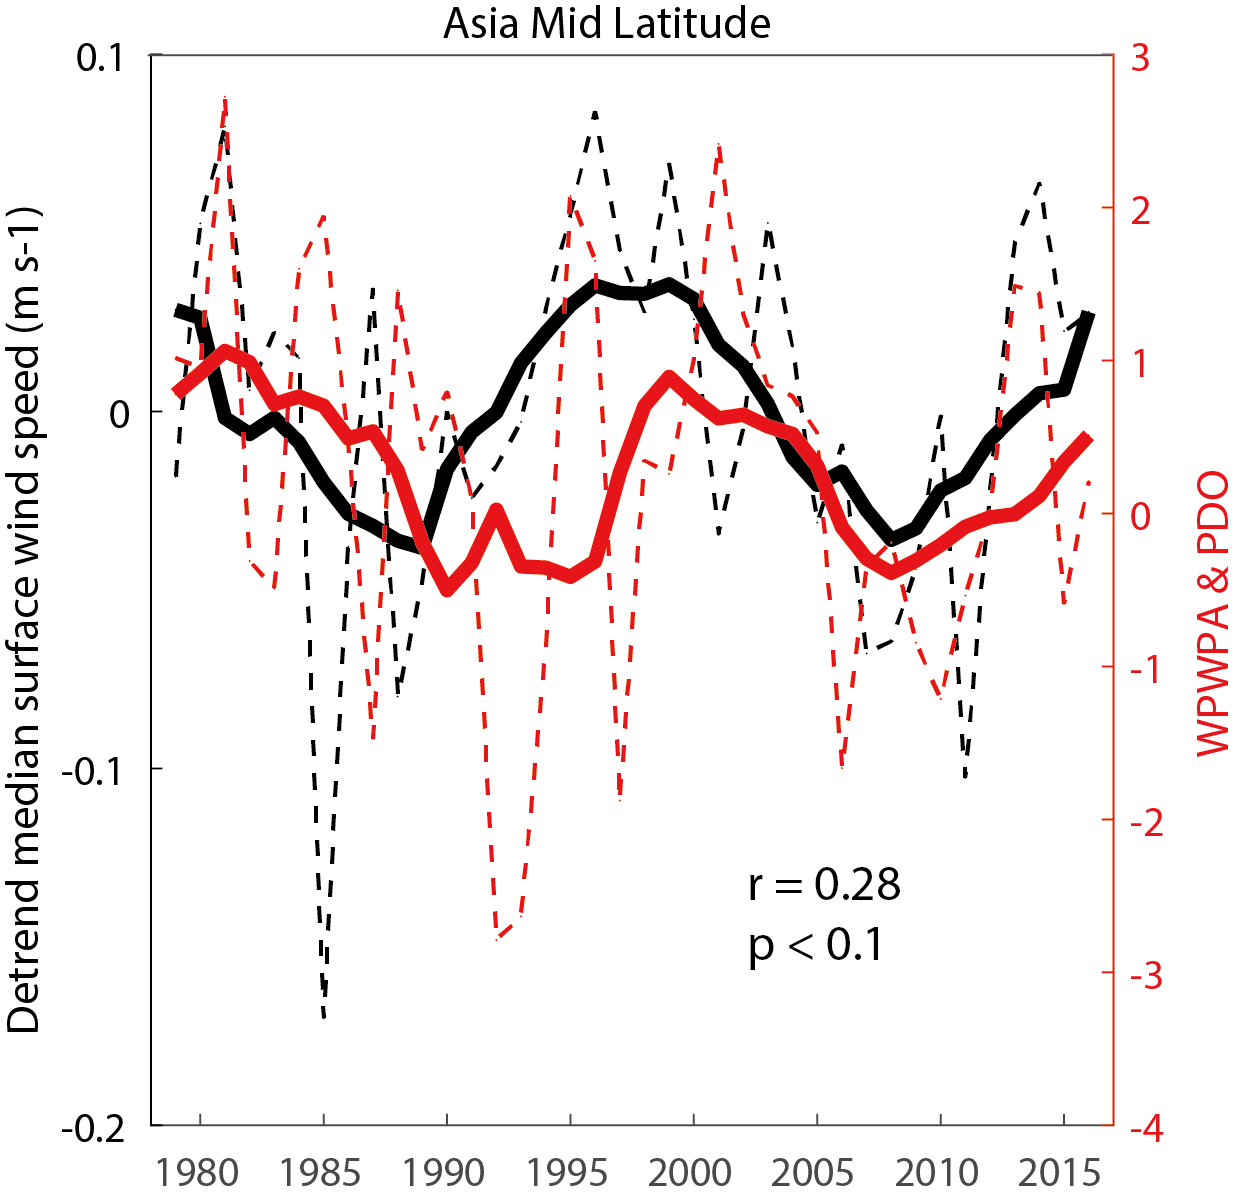
\includegraphics[width=0.45\textwidth]{亚洲中纬度风速与WPWPA和PDO}
    \bicaption{ 亚洲中纬度风速与西太平洋暖池面积指数(WPWPA)和PDO指数演变。黑色(红色)虚线为亚洲中纬度地区中位数风速(PDO指数年均值 $\times$-0.88 $+$ 去趋势WPWPA指数年均值 $\times$ -1.44),实线为虚线9年滑动平均结果,两实线的相关系数为0.28,p < 0.1。}{Evolution of Asian mid latitude wind speed, WPWPA index and PDO index. Black (red) dash line is Asian mid latitude annual median wind speed (annual mean value of PDO index $\times$ -0.88 $ + $ detrend annual mean value of WPWPA index $\times$ -1.44 ), solid line is 9-point moving mean of dash line, correlation coefficient between two solid lines is 0.28, p < 0.1.}
    \label{fig:ASwindspeedPDOandWPWPA}
\end{figure}

\section{本章小结}

本章从大气运动驱动力的变化出发,分析了对流层风速的变化,气压场变化,大尺度海温和环流系统对于陆地地表风速的影响,得到以下主要结论:

\begin{enumerate}

\item 在欧洲和亚洲中纬度地区,对流层低层风速都出现了下降,因而这两个地区地表风速下降可以由高空风速下降部分解释,但高空风速下降的速度远小于地表,因而高空风速变化不是地表风速下降的主要原因。而在北美洲和亚洲低纬度地区,对流层低层风速都出现了上升,尤其是北美洲,几乎所有探空站点都表现出风速上升,因而这两个地区地表风速下降难以由高空风速变化解释。无论在在北美洲、欧洲、亚洲低纬度和中纬度地区,地表与高层风速年代际变化均没有表现出很好的一致性。

\item 1月海平面气压场变化主要表现为冰岛低压减弱、西伯利亚高压北部增强和阿留申低压向西北偏移,会使得南欧和北美风速减小,而北欧和亚洲风速增加。7月海平面气压场变化主要表现为冰岛低压增强,会使得南欧风速增加而北欧风速减小。

\item 北美洲和欧洲陆地地表风速年代际变化分别受到TNA和NAO的显著影响,亚洲中纬度陆地地表风速年代际变化受到PDO和西太平洋暖池面积的共同影响。

\end{enumerate}
%  --------------------- chapter 4--------------------- %
\chapter{大气运动阻力变化对陆地地表风速长期变化的影响}\label{chap:dragingforceonwind}

\section{引言}

第\ref{chap:drivingforceonwind}章从大气运动驱动力变化的角度分析了陆地地表风速长期变化的原因,本章将从大气运动阻力变化的角度进行分析。

土地利用的变化是大气运动阻力变化的主要原因之一。如第\ref{chap:intro}章所述,已有许多相关研究分析了土地利用变化对于陆地地表风速的影响\citep{vautard2010northern, wu2016estimating, kalnay2003impact, guo2011changes}。以往的研究主要采用对比城市与乡村站点风速变化,建立参考序列与观测序列对比,或是建立简化动力模型和数值模拟的方法。其中,许多以往研究将观测站点分为城市站点和乡村站点(通常是基于人口),通过比较两类站点的风速趋势差别来确定城市化对于风速的影响\citep{guo2011changes}。这种方法能够成立基于以下假设:城市站点周边建设用地增加总是显著快于乡村站点周边,而同时乡村站点周边建设用地增加几乎可以忽略,即人口多的地区的城市化速度显著快于人口少的地区。然而这个假设存在一定问题,更好的方式是通过计算城市人口或建设用地的动态变化来确定城市化的速度。此外,也有研究通过建立不受土地利用变化影响的参考序列,并对比观测序列来考察土地利用变化的影响。有些再分析资料(如NCEP/NCAR)没有同化陆地观测资料,因而被认为可以作为参考序列\citep{kalnay2003impact}。\citet{zha2017effects}将此思路用于了土地利用变化对中国东部地区风速的影响。这种方法能一定程度上反映土地变化的作用,但即便同样是没有同化地表风速观测的再分析资料之间,对于地表风速变化也存在很大分歧(参见第\ref{chap:SpatiotemporalCharacteristics}章),因而这种方法的可靠性也在疑问。另外一种方式是利用简化动力学模型(形式类似于第\ref{chap:intro}章公式 \ref{eq:winddynmaic}),将土地利用的影响简化为拖拽系数的变化(例如\citet{wu2016estimating}),这种简化不一定能够代表土地利用变化对于边界层内湍流混合过程的复杂影响,因而对分析结果造成一定的不确定性。也有研究尝试用数值模拟的手段进行研究,但这些研究多是采用假设的土地利用变化情景而不是真实的土地利用变化进行研究(例如\citet{vautard2010northern})。由此,为了克服前人研究的不足,本章先是利用动态的土地利用数据与风速观测数据进行统计分析,然后设计数值试验考察真实的土地利用变化对于风速的影响。由于模拟城市化、植被变化等对气候的影响需要很高分辨率(1~5 $km$ 水平分辨率),对计算资源的消耗巨大,因而难以进行大尺度的模拟。因此,本章的数值试验选取在城市化和植被变化明显的代表性区域进行。

大气运动的动量由边界层以上的自由大气向边界层内传递主要依赖湍流混合过程。垂直温度递减率是影响湍流强度的主要变量之一,原因是垂直温度递减率的改变会引起大气稳定度变化,当下层增温超过上层时气块会在浮力的作用下形成不稳定运动\citep{J2004An}。\citet{gaffen2000multidecadal}发现,1979-2000年间地表附近的增暖快于对流层低层,表明边界层稳定度增加。据我所知,目前还没有研究分析近几十年来大尺度的边界层垂直温度递减率变化,本章将对这个问题进行分析。

\section{资料和方法}

本章使用了以下数据集:
NCEI-CMDC陆地地表风速观测数据集。此数据集的相关信息已在第\ref{chap:SpatiotemporalCharacteristics}章中做过描述,这里不再重复。本章使用此数据进行大尺度长期风速变化的分析。

中国地面气候资料日值数据集(V3.0)。此数据集同样在第\ref{chap:SpatiotemporalCharacteristics}章中已有介绍。本章将此数据集经过均一化处理后(处理方法将在下文详细介绍)用于珠江三角洲风速长期变化的分析。之所以在此区域的分析中没有使用NCEI-CMDC数据集是由于此数据集由于严格的质量控制过程剔除了大量站点,使得珠江三角洲的风速观测序列只有一个,以此分析珠江三角洲风速长期变化不确定性很大。而相比之下,经过均一化之后的中国地面气候资料日值数据集在珠江三角洲有6个站点,分析结果的不确定性大大降低。

\href{http://www.resdc.cn}{中国土地利用/土地覆盖遥感监测数据集} 由中国科学院资源环境科学数据中心制作,包含20世纪70年代末期、80年代末期、90年代中期、90年代末期、2005年、2010年和2015年7个时期中国土里利用/土地覆盖数据,空间分辨率为1 $\times$ 1 $km$。此数据集使用Landsat遥感影像数据制作而成,包含耕地、林地、草地、水域、城乡工矿居民用地、未利用土地6个大类和25各小类。本章使用了20世纪70年代末和2015年土地利用数据作为数值模拟的边界条件进行珠江三角洲城市化对于风速长期变化影响的数值试验。

MODIS12Q1土地利用数据集\citep{sullamenashe2019hierarchical}由美国宇航局(NASA)制作,包含全球2001年至今每年500 $\times$ 500 $m$分辨率土地利用数据。此数据集使用Terra和Aqua卫星上搭载的中分辨率成像光谱仪(MODIS)传感器数据制作而成,包含IGBP、UMD、LAI、BGC和PFT等5个分类标准下的土地利用数据。本章使用了2001年和2016年土地利用数据作为数值模拟的边界条件进行芬兰南部植被变化对于风速长期变化影响的数值试验。

\href{http://www.atlasofurbanexpansion.org/data}{Atlas of Urban Expansion城市变化数据集} 由纽约大学(NYU)制作,包含20世纪80年代至21世纪前10年全球200个城市发展的动态数据,包括人口、城市建设面积、街区和道路等。此数据集使用Landsat遥感影像数据制作而成。本章使用了全球200个城市的城市建设面积动态数据分析城市化与风速长期变化的关系。

\href{https://climatedataguide.ucar.edu/climate-data/ndvi-normalized-difference-vegetation-index-3rd-generation-nasagfsc-gimms}{GIMMS NDVI 3g}由NASA制作,包含全球1981年至2015年0.083 $\times$ 0.083度归一化植被指数(NDVI)数据。此数据集由卫星上搭载的超高分辨率辐射计(AVHRR)数据制作而成,NDVI计算公式如下:

\begin{equation} \label{eq:ndvi}
NDVI = \frac{NIR - VIS}{NIR + VIS}
\end{equation} ~\\
其中NIR表示近红外光反射率,VIS表示可见光反射率。健康的植被会吸收大部分可见光,而反射大部分近红外光,然而不健康或者稀疏的植被会反射更多可见光和更少近红外光。NDVI的范围是-1 \textasciitilde 1,当没有绿叶存在时NDVI接近于0,当绿叶密度非常高时NDVI接近1。本章使用1982和2015年NDVI数据分析植被变化与风速长期变化的关系。

HadGHCND全球地表温度观测数据集\citep{caesar2006large-scale}由哈德莱中心制作,包含全球1950年至今2.5纬度$\times$3.75经度分辨率日最高和最低温度观测数据。此数据集由NCEI等全球历史气候网络(GHCN)日观测数据集制作而成,制作过程中包含了质量控制步骤以减少错误和可疑数据等影响,并使用角度-距离加权算法将站点数据插值到格点。本章使用1979-2012年地表日最高气温分析边界层日间垂直温度递减率变化。

HadAT全球对流层温度数据集\citep{thorne2005revisiting}由哈德莱中心制作,包含全球1985-2012年5纬度$\times$10经度分辨率对流层850、700、500、300、200、150、100、50和30 $hPa$共9个层次的月平均温度。此数据集由676个探空站点数据制作而成,由于这些探空站点多分布于北半球,因而此数据集有效数据也多集中于北半球。制作过程中使用了质量控制步骤来减小仪器和观测方式等变化的影响。本章使用了1979-2012年850 $hPa$温度数据分析边界层垂直温度递减率的变化。

本章使用了RHtest V4观测序列均一化算法\citep{wang2014rhtests}对风速观测序列进行均一化处理。此算法基于penalized maximal t test\citep{wang2007penalized}和penalized maximal F test\citep{wang2008penalized},可以在有参考序列和没有参考序列的情况下检测观测序列的异常突变点,并进行修正,修正方式包括均值修正和Quantile-Matching(QM)修正,后者既可以调整均值也可以使突变点前后的经验分布一致\citep{wang2010new},获得广泛应用\citep{vincent2012second, baule2014climatology, yang2019causes}。本章在处理珠江三角洲风速数据时使用ERA-Interim 10 $m$风场资料作为参考序列检测观测序列的突变点,并使用QM修正,最后用人工检查确认突变点检测和修正无明显不当之处。

本章数值试验使用了WRF-ARW 4.0\citep{skamarock2019description},此模式是由美国国家大气研究中心(NCAR)开发的下一代中尺度数值天气预测系统,是目前模拟效果最好、应用最广泛的中尺度天气数值模式。本章的数值试验使用FNL作为初始和边界条件,分别针对城市化和植被变化在珠江三角洲和芬兰南部进行了两组数值试验,模式参数设置和数值试验设计将在下文中详细描述。

本章计算趋势和相关系数以及统计显著性水平的方法与第\ref{chap:SpatiotemporalCharacteristics}、\ref{chap:drivingforceonwind}章相同。RMSD计算方法如下:

\begin{equation} \label{eq:rmsd}
RMSD = \frac{\frac{1}{N} \sum_{n=1}^{N} \left( c_{n} - \bar{c} \right) \left( d_{n} - \bar{d} \right) }{\sigma_{c} \sigma_{d}}
\end{equation} ~\\
其中$\bar{c}$和$\bar{d}$分别为空间场c和d的均值,$\sigma_{c}$和$\sigma_{d}$为c和d的标准差。

\section{城市化的影响} \label{sec:urbanimpact}

\subsection{基于城市动态变化和风速观测数据的统计学分析}

\begin{figure}[!htbp]
    \centering
    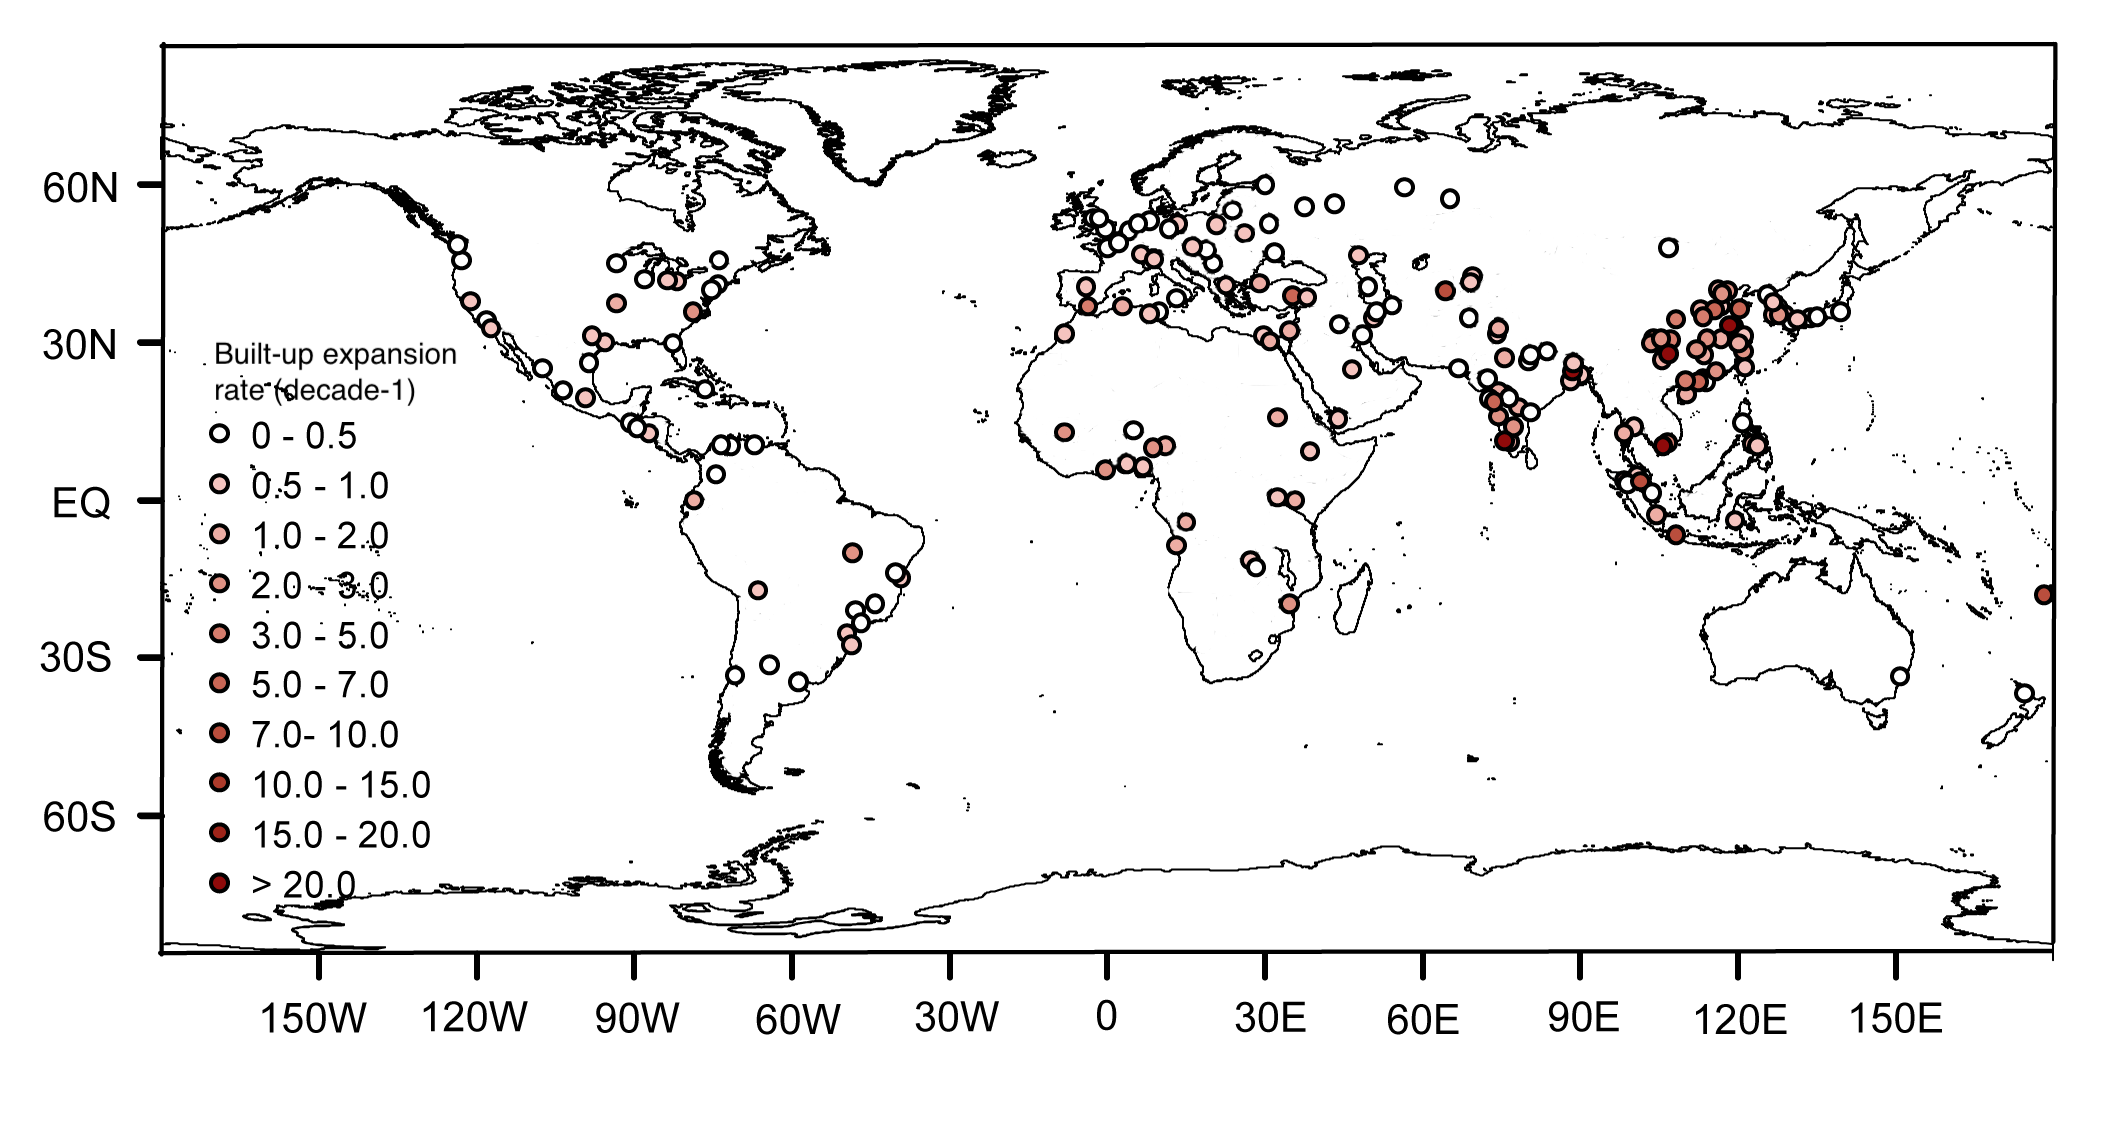
\includegraphics[width=1\textwidth]{城市扩张速度}
    \bicaption{ 城市扩张速度(变化率 每十年)}{City expansion rate (in $changing ~ rate ~ per ~ decade$)}
    \label{fig:cityexpansionrate}
\end{figure}

%\setupctable{captionsleft}% 标题朝向
\begin{figure}[!htbp]
    \centering
    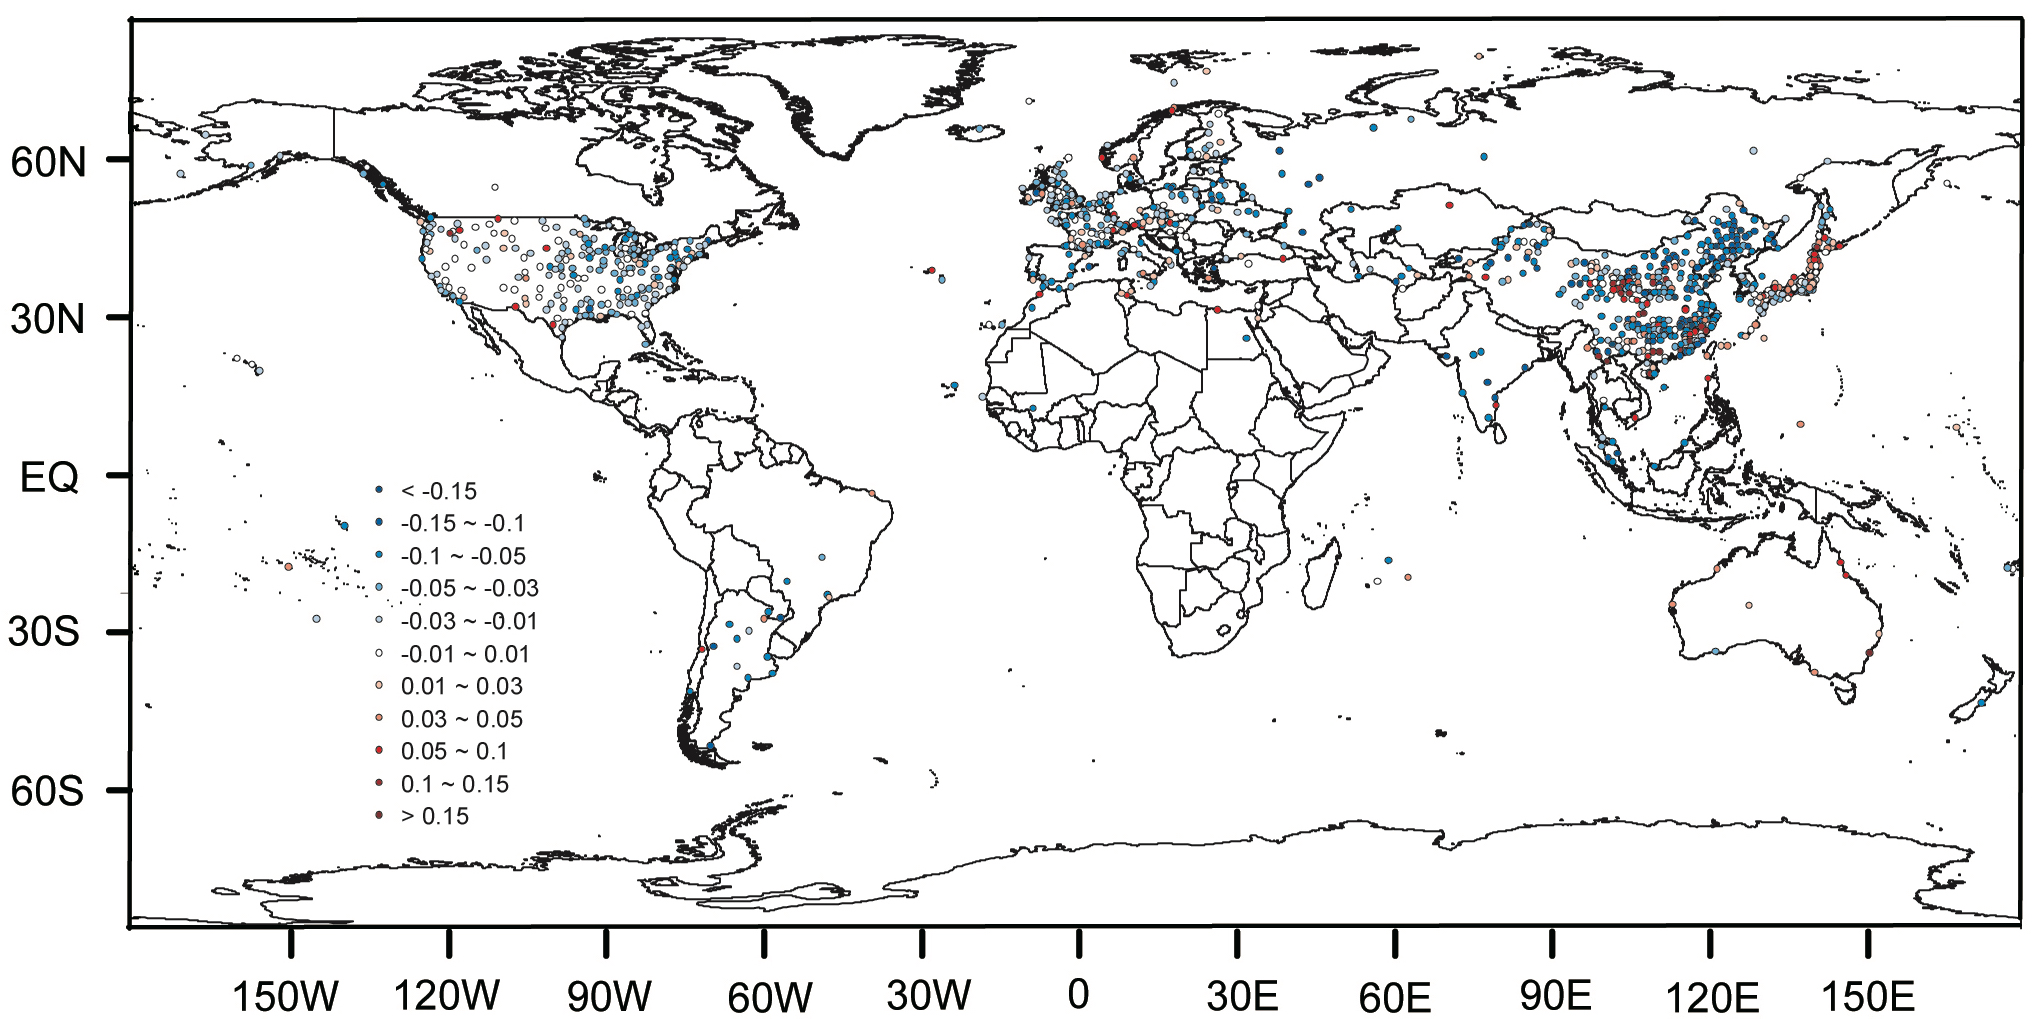
\includegraphics[width=1\textwidth]{归一化地表风速趋势}
    \bicaption{ 归一化地表风速趋势(变化率 每十年)}{Normalized surface wind speed trends (in $changing ~ rate ~ per ~ decade$)}
     \label{fig:normalizedwindtrend}
\end{figure}

\begin{figure}[!htbp]
    \centering
    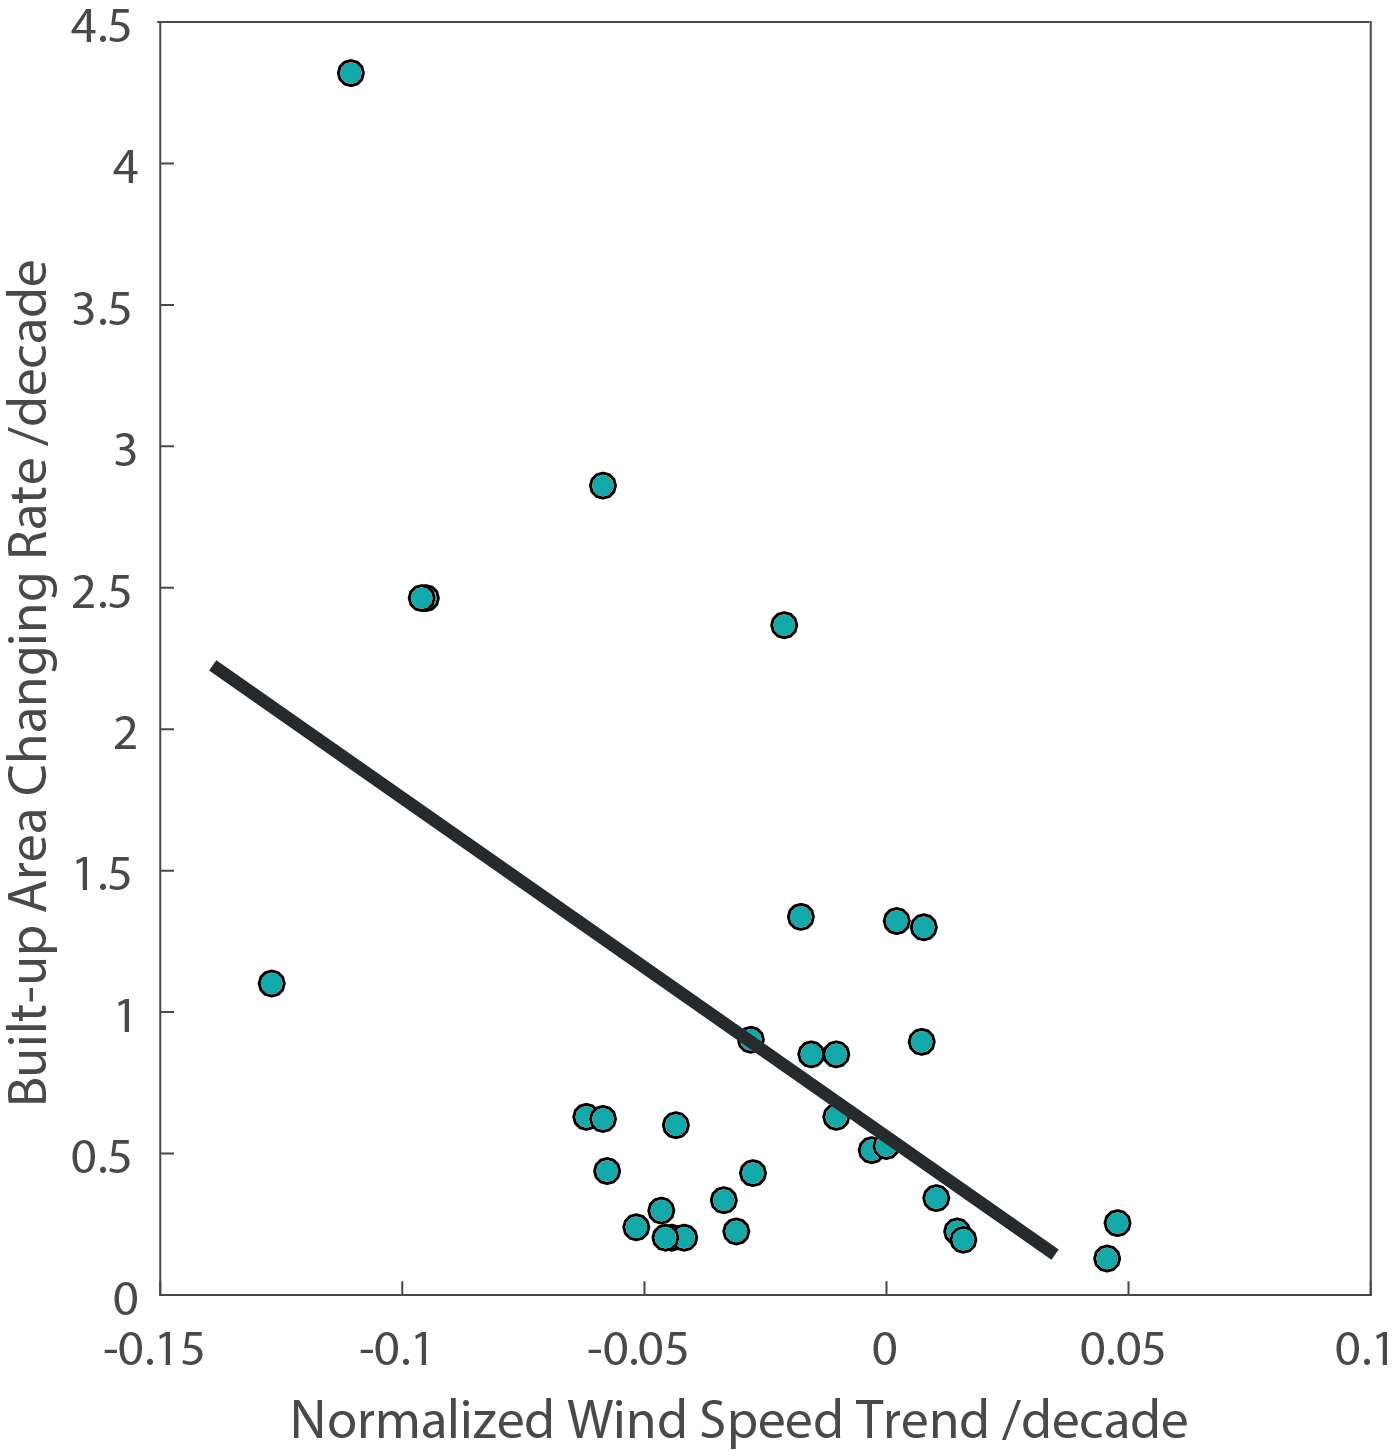
\includegraphics[width=0.5\textwidth]{城市扩张与风速变化}
    \bicaption{ 城市扩张速度与对应地区风速变化}{City expansion versus wind speed change in the corresponding area.}
    \label{fig:cityexpansionvswindchange}
\end{figure}

\begin{figure}[!htbp]
    \centering
    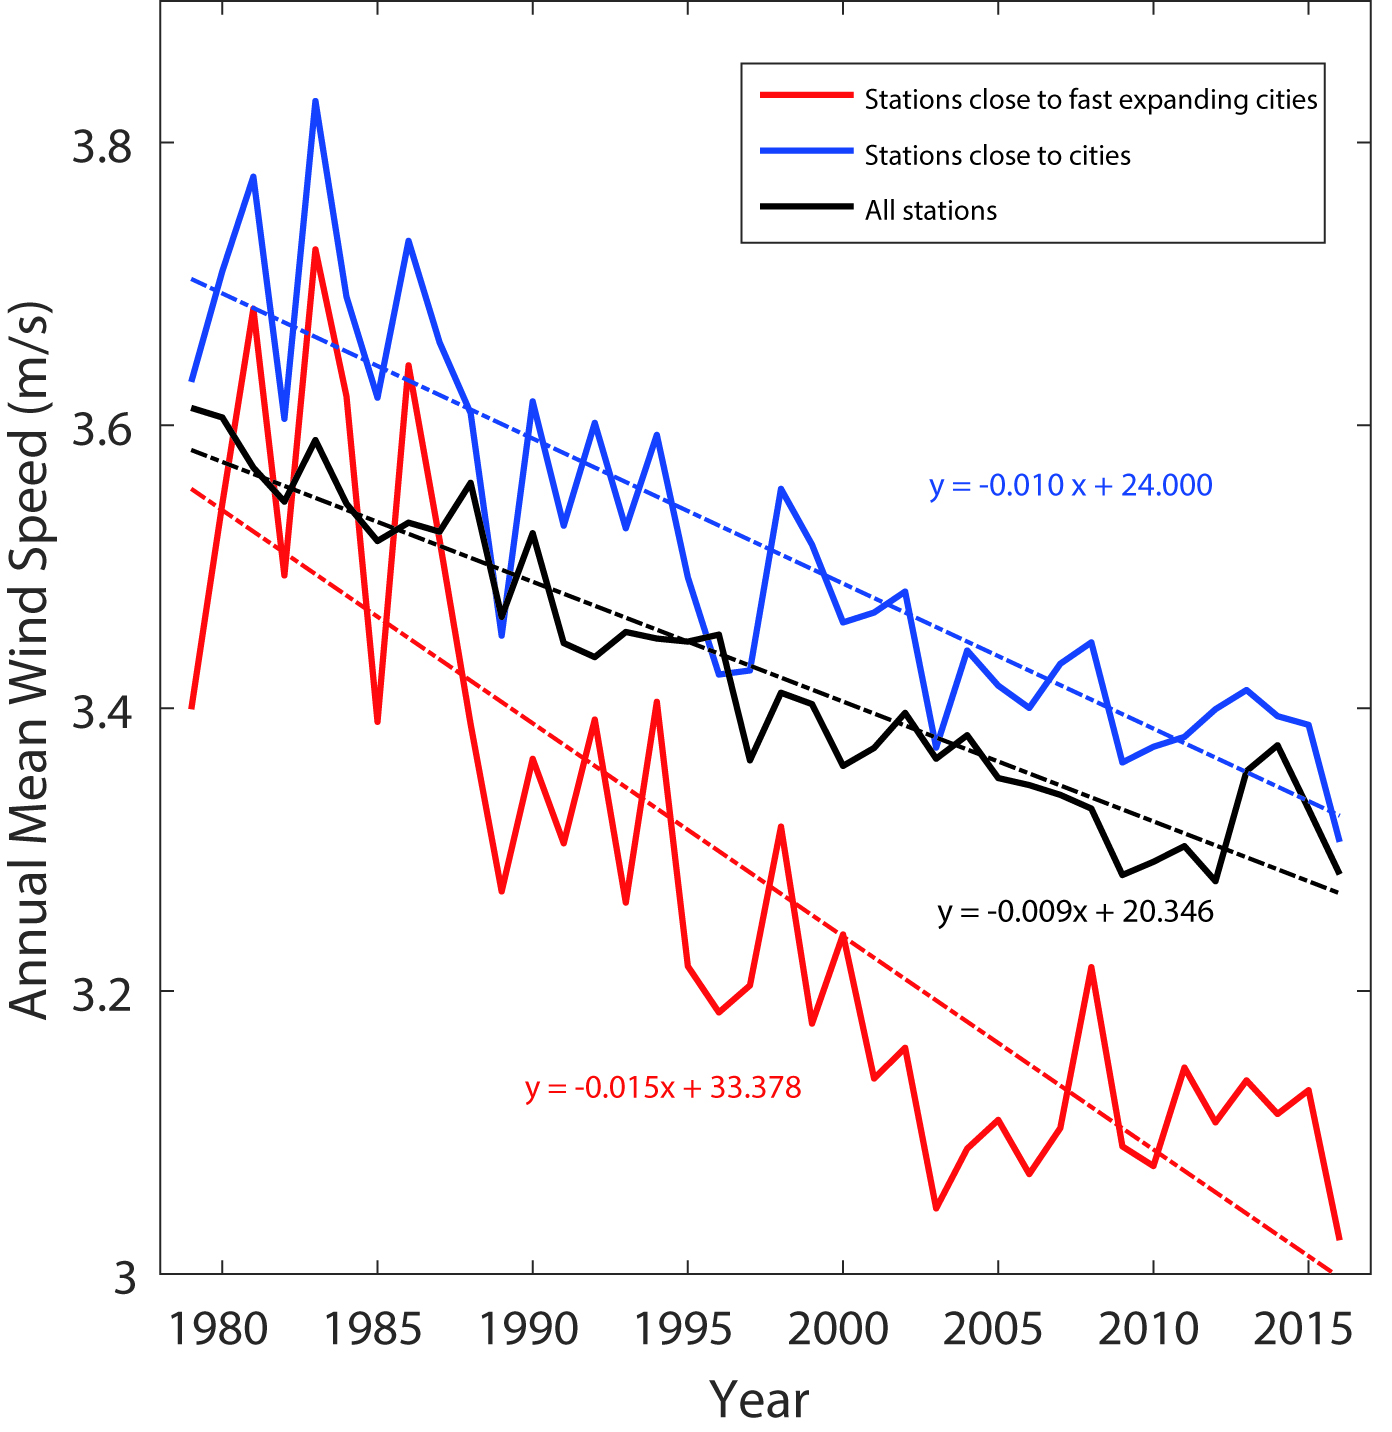
\includegraphics[width=0.5\textwidth]{不同城市化速度风速对比}
    \bicaption{ 不同城市化速度地区风速演变。红色实线为快速城市化的城市附近站点风速演变,蓝色实线为所有靠近城市站点风速演变,黑色实线为所有站点风速演变。虚线为对应实线的线性趋势。}{Wind speed evolution under different urbanization rates. Red solid line is evolution of wind speed near fast urbanizing cities, blue solid line is evolution of wind speed near all cities, black solid line is evolution of wind speed across the world. Dash lines are trends for solid lines.}
    \label{fig:windunderdiffurban}
\end{figure}

使用Atlas of Urban Expansion数据计算城市建设面积自20世纪80年代至21世纪前10年的变化率,发现所有200个城市建设面积都有增加,其中62\%增加速度超过50\% 每十年,36\%超过100\% 每十年,增加最快的中国江苏盱城和孟加拉国Rajshahi增加速度超过4000\% 每十年。相比之下,北美洲和欧洲城市建设面积增加速度较慢,原因是欧美发达国家的城市化在更早时候就已经基本完成,而亚洲的中国、印度和东南亚各国,近30多年来城市化进程非常迅速(图 \ref{fig:cityexpansionrate})。对比使用NCEI-CMDC风速数据计算的1979-2016年归一化风速趋势,发现亚洲整体风速下降速度大于欧洲和北美(图 \ref{fig:normalizedwindtrend}),似乎预示着城市化在其中起到了一定作用。选择距离城市中心0.15度(约15 $km$)以内的观测站点,将地表风速趋势与城市建设面积变化速度对比,发现二者有显著的负相关(p < 0.01),即城市扩张越快的地区,风速越趋向于减小(图 \ref{fig:cityexpansionvswindchange})。对比上述城市中心附近站点中城市扩张速度在前50\%的风速趋势,所有城市中心附近站点风速趋势和所有站点风速趋势发现,所有城市中心附近站点和所有站点平均风速趋势接近,分别为-0.1 和 -0.09 $m ~ s^{-1}$每十年,相比之下快速扩张城市周边站点风速趋势则小得多,达到-0.15 $m ~ s^{-1}$每十年(图 \ref{fig:windunderdiffurban})。由此说明城市化进程会使得附近的风速显著减小。

\subsection{数值试验}

为了进一步验证城市化与风速变化的关系,使用WRF-ARW 4.0进行数值试验,选择中国东南沿海的珠江入海口附近的珠江三角洲作为模拟区域(图 \ref{fig:PRDlocation}),因为它包含广州、深圳、珠海、香港、澳门等城市,是中国近30多年来城市化最快的地区之一(图 \ref{fig:PRDcityexpand}),而中国是全球近30多年来城市化最快的国家之一。此地区地势较为平坦,海拔高度基本在800 $m$以下 (图 \ref{fig:PRDlocation})。

\begin{figure}[!htbp]
    \centering
    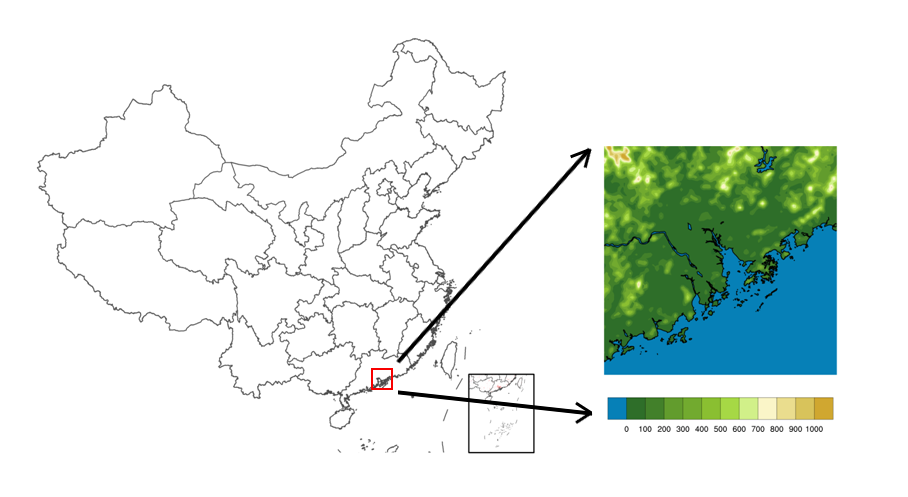
\includegraphics[width=0.9\textwidth]{珠江三角洲地理位置}
    \bicaption{ 珠江三角洲地理位置}{Location of the Pearl River Delta.}
    \label{fig:PRDlocation}
\end{figure}

\begin{figure}[!t]
    \centering
    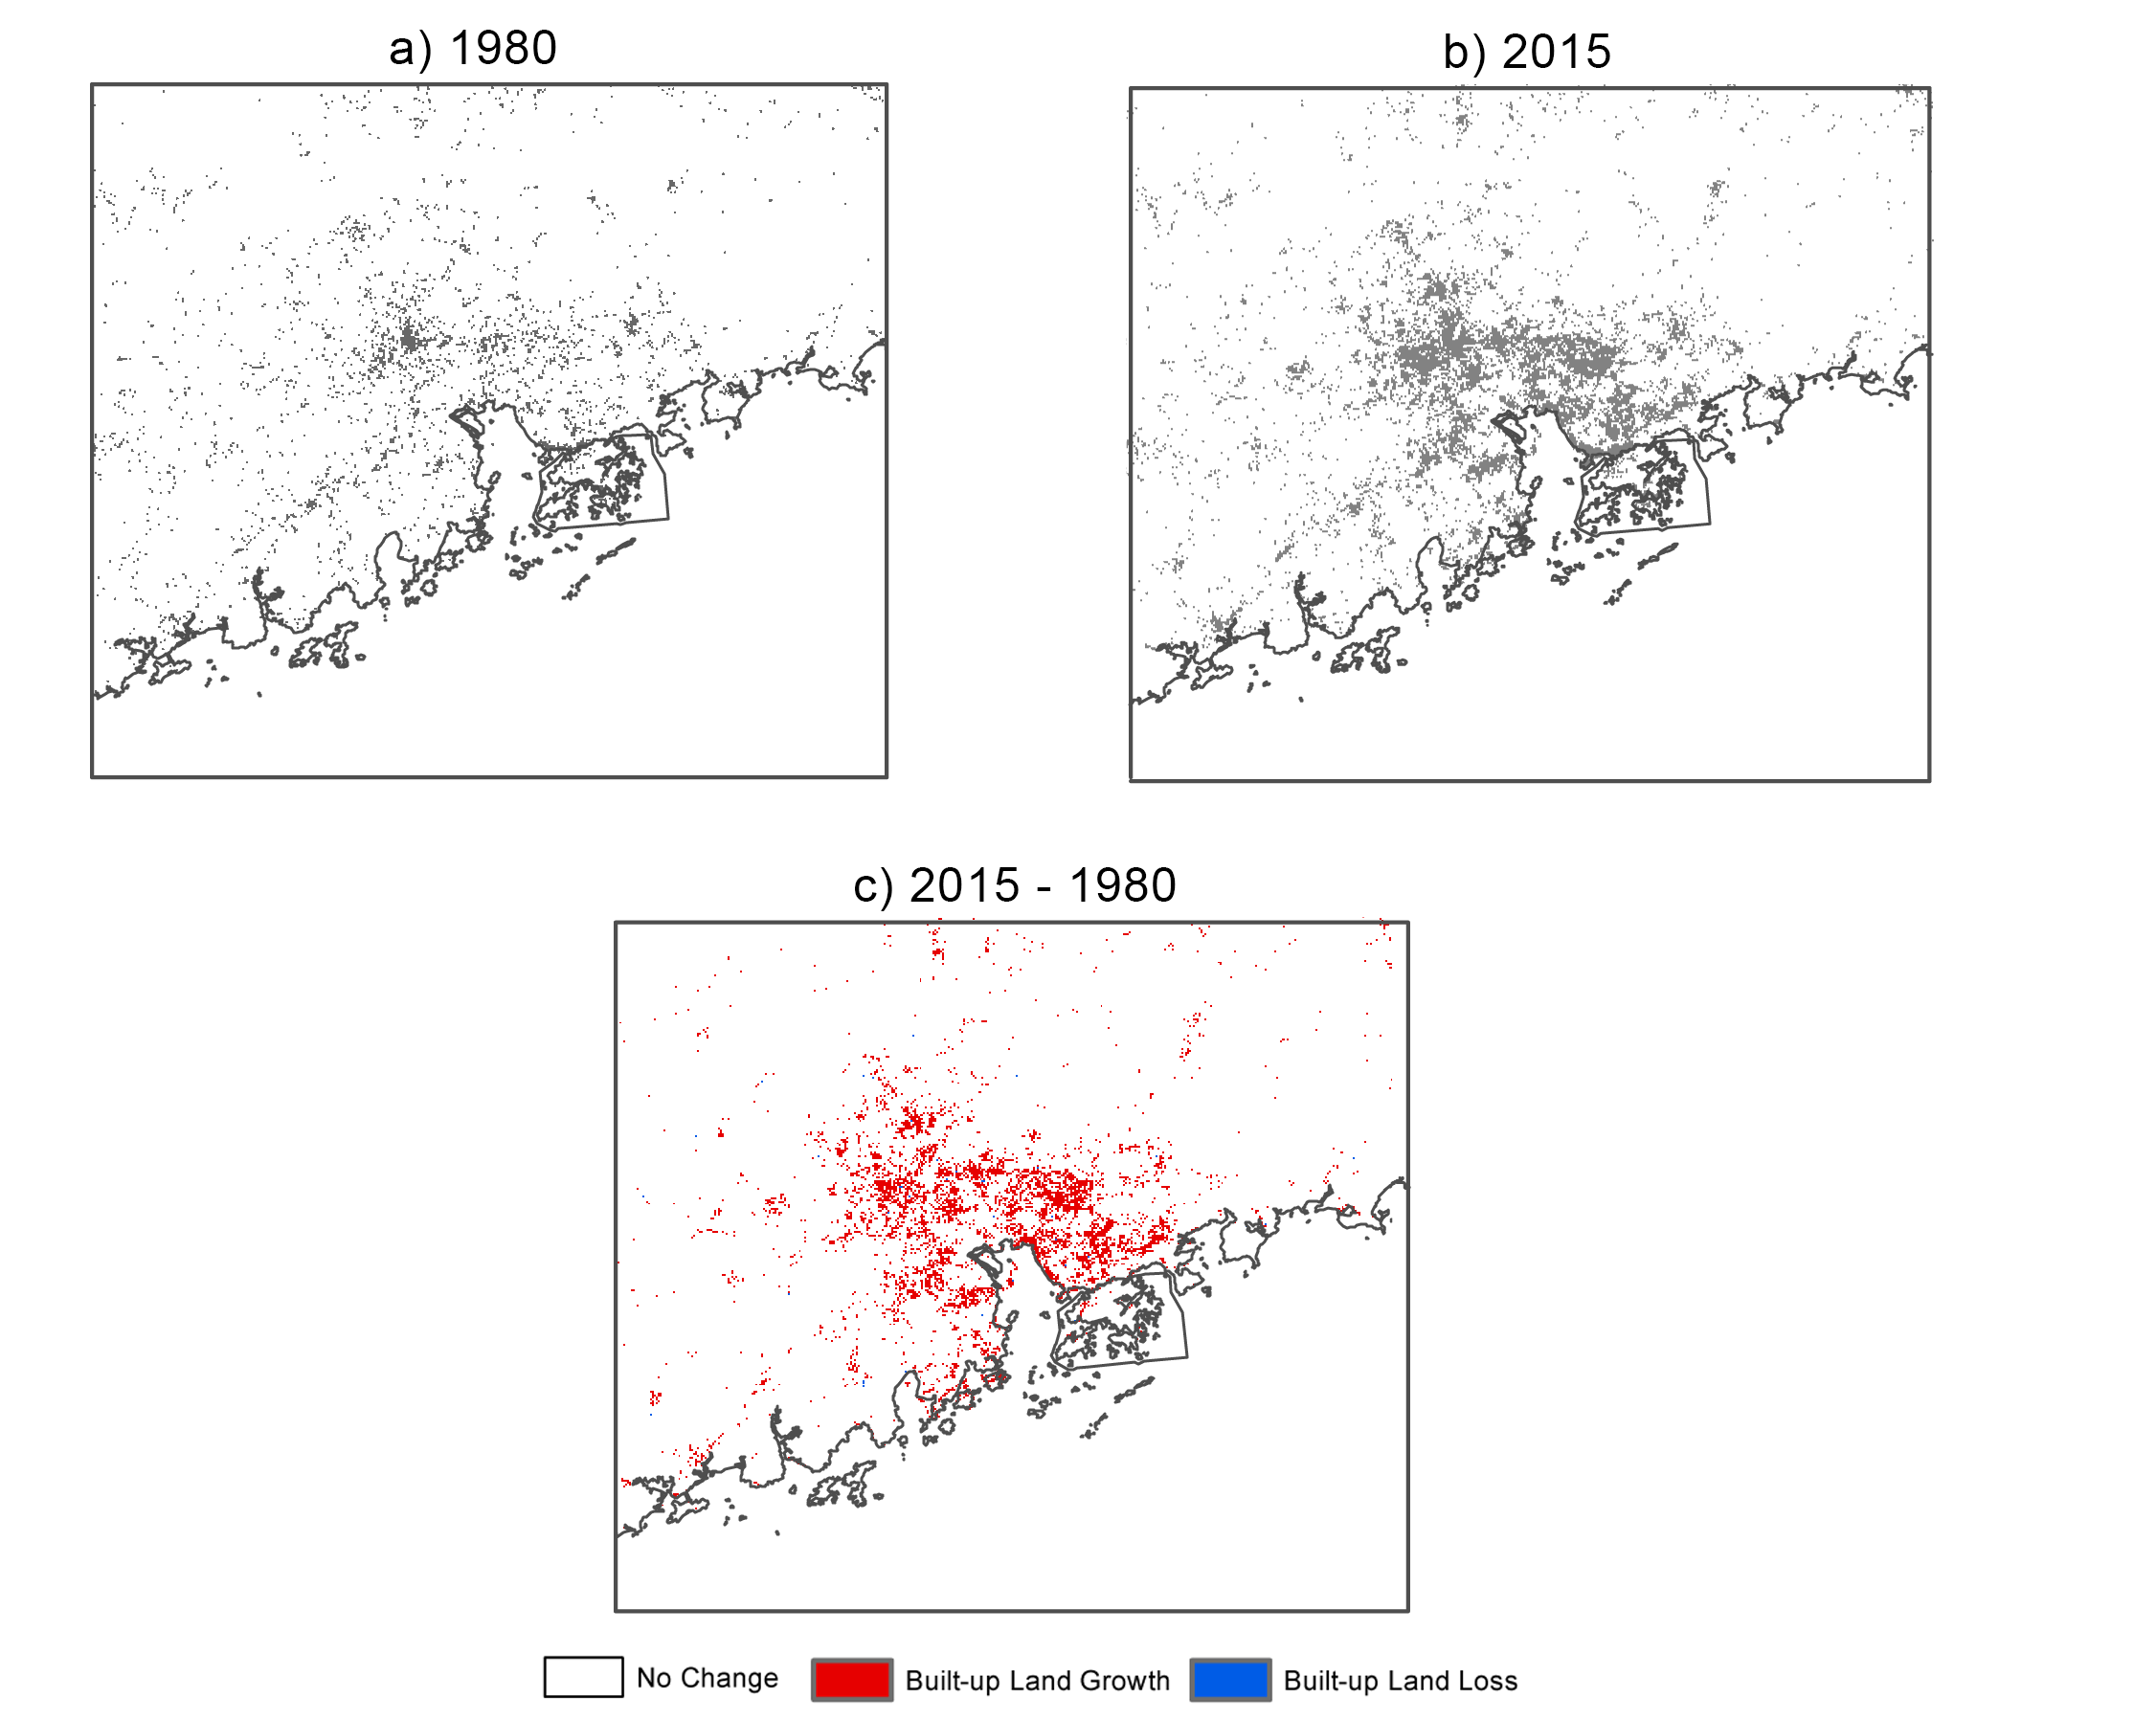
\includegraphics[width=1\textwidth]{珠江三角洲城市扩张}
    \bicaption{ 珠江三角洲城市扩张。a)1980年城市范围,b)2015年城市范围,c)2015年相对1980年城市范围的变化,白色表示没有变化,红色表示增加,蓝色表示减少。}{City expansion in the Pearl River Delta. a)Built-up extension in 1980, b)Built-up extension in 2015, c)Built-up change from 1980 to 2015, white color denotes no change occurred, red denotes add, blue denotes lose.}
    \label{fig:PRDcityexpand}
\end{figure}

将模式设置为三层双向嵌套,空间分辨率分别为30 $km$、10 $km$和3.3 $km$(图 \ref{fig:PRDmodeldomain}),垂直包含40个层次,其中边界层内(1km高度以下)10个层次;时间步长为100 $s$;微物理参数化方案为WRF Single-Moment 6-class scheme \citep{hong2006the};积云参数化方案为Grell 3D \citep{grell1993prognostic, grell2002a},在较高分辨率的两层网格关闭积云参数化;云量使用Xu-Randall method \citep{xu1996a};长波辐射参数化方案为RRTM scheme \citep{mlawer1997radiative},短波辐射参数化方案为Dudhia scheme \citep{dudhia1989numerical};边界层采用BouLac PBL \citep{bougeault1989parameterization},陆面模式选择Noah-MP \citep{niu2011the};城市参数化方案采用Building Environment Parameterization (BEP) \citep{salamanca2010a}。

\begin{figure}[!htbp]
    \centering
    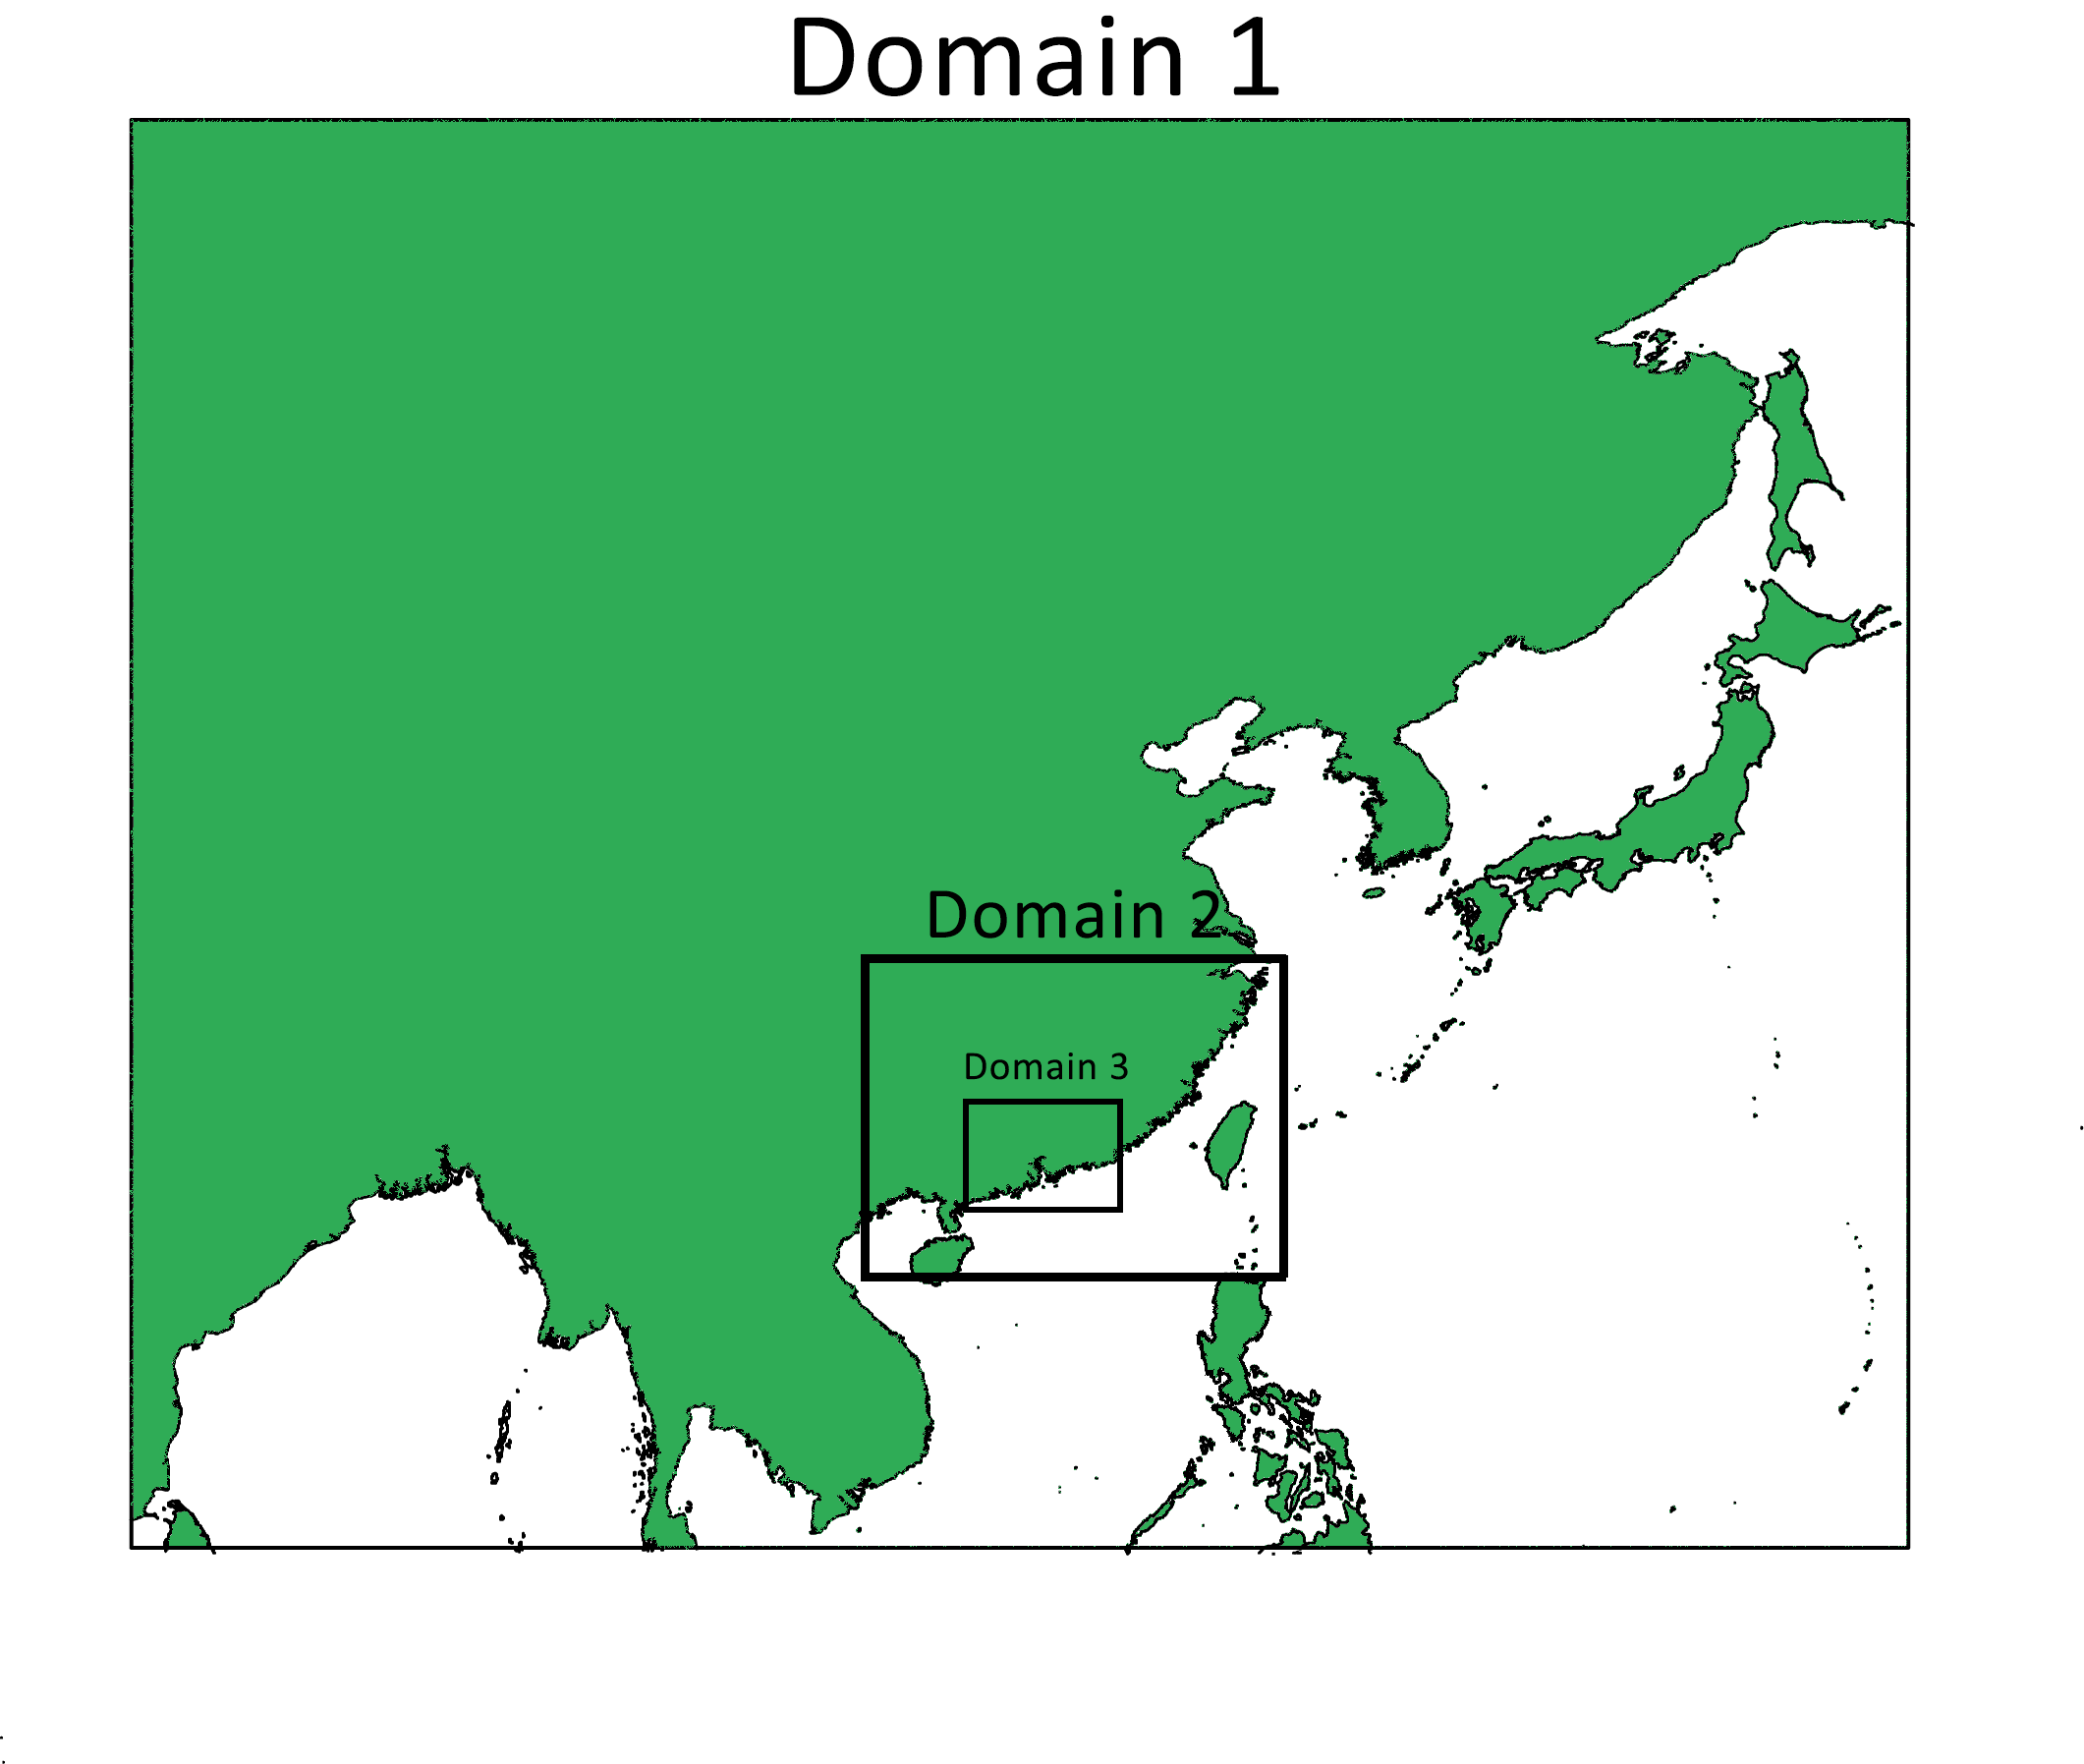
\includegraphics[width=0.7\textwidth]{模拟区域}
    \bicaption{模拟区域}{Model simulation domains}
    \label{fig:PRDmodeldomain}
\end{figure}

采用以上模式设置进行三组模拟,分别为:

\begin{enumerate}

\item \label{sim:1.1} 以华南地区20世纪70年代末土地利用类型(来自中国土地利用/土地覆盖遥感监测数据集)作为下边界条件进行模拟。

\item \label{sim:1.2} 以华南地区20世纪70年代末土地利用类型叠加2015年珠江三角洲地区建设用地范围作为下边界条件进行模拟。
	
\item \label{sim:1.3} 以华南地区2015年土地利用类型作为下边界条件进行模拟。

\end{enumerate}

\begin{figure}[!htbp]
    \centering
    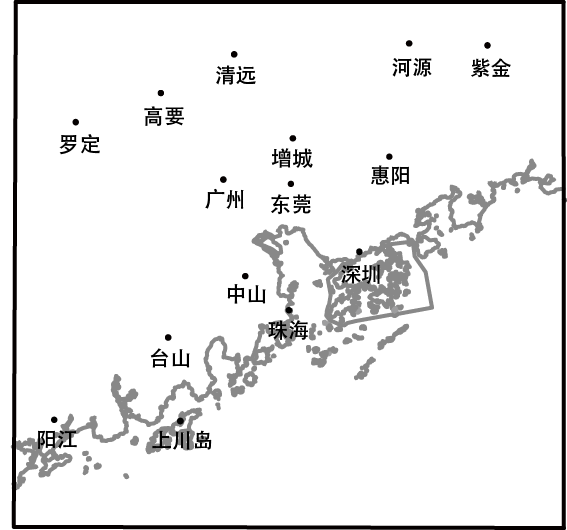
\includegraphics[width=0.5\textwidth]{珠江三角洲测站位置}
    \bicaption{ 珠江三角洲测站位置}{Observation stations in the Pearl River Delta.}
    \label{fig:PRDobssites}
\end{figure}

对以上三组模拟,气象场采用FNL2015年6月和2015年12月(分别代表珠江三角洲雨季和旱季)1 $\times$ 1度6小时分辨率物理量场,经确认,在模拟时段内无台风和寒潮过程发生。模式积分过程分为3段,每段约10天。

使用模拟\ref{sim:1.3}结果对比观测进行模式性能评估,珠江三角洲及周边区域地面观测站点位置和信息可在图 \ref{fig:PRDobssites}和表 \ref{tab:PRDsiteinfo}找到。对比模拟与观测结果,发现模拟风速普遍大于观测,这在以往的研究中也被发现\citep{zhang2010modeling, yu2015evaluation, zha2019numerical}。为了减少这种模拟偏差的影响,在模拟结果的分析时,应使用归一化风速变化而不是风速变化的绝对值。模拟与观测风速体现出了很好的相关,说明模拟结果可以很大程度上抓住风速的时间变化。RMSD结果对比以往研究\citep{zhang2010modeling, zha2019numerical}也表明模式对珠江三角洲区域风速有较好的模拟效果(表 \ref{tab:PRDsiteinfo})。

\begin{table}[!htbp]
    \bicaption{珠江三角洲站点信息及模式性能评估结果}{Description of observation stations in the Pearl River Delta and model validation results}
    \label{tab:PRDsiteinfo}
    \centering
    \small% fontsize
    \setlength{\tabcolsep}{5 pt}% column separation
    \renewcommand{\arraystretch}{1.0}%row space 
    \begin{tabular}{lccccccc}
        \hline
        站名 & 站号 & 纬度 & 经度 & 海拔($m$)&  \multicolumn{3}{c}{10 $m$ 风速} \\
         & & & & & 均值($m ~ s^{-1}$)$^*$ &  相关系数 $^ {**}$ & RMSD \\
        %\cline{2-9}% partial hline from column i to column j
        \hline
        高要 & 59278 & 23.02 & 112.27 & 41.9 & 3.7(-1.8) & 0.07 & 1.21 \\
        清远 & 59280 & 23.43 & 113.05 & 79.2 & 3.4(0.1) & \textbf{0.39} & 0.95 \\
        广州 & 59287 & 23.13 & 113.29 & 70.7 & 2.9(-0.4) & \textbf{0.40} & 0.65 \\
        东莞 & 59289 & 22.58 & 113.44 & 56.8 & 2.3(0.5) & \textbf{0.44} & 0.54 \\
        河源 & 59293 & 23.48 & 114.44 & 71.6 & 4.1(-2.1) & \textbf{0.59} & 1.10 \\
        增城 & 59294 & 23.20 & 113.50 & 31.5 & 4.4(-2.0) & \textbf{0.34} & 1.40 \\
        惠阳 & 59298 & 23.04 & 114.22 & 109.3 & 3.2(-0.6) & \textbf{0.55} & 1.23 \\
	   紫金 & 59304 & 23.38 & 115.11 & 177.6 & 3.0(-1.4) & \textbf{0.38} & 0.77 \\
	   罗定 & 59462 & 22.42 & 111.36 & 60.9 & 2.3(-0.7) & 0.21 & 0.89 \\
	   台山 & 59478 & 22.15 & 112.47 & 33.7 & 4.0(-1.4) & \textbf{0.47} & 0.70 \\
	   中山 & 59485 & 22.3 & 113.24 & 34.5 & 3.2(-1.0) & \textbf{0.35} & 0.87 \\
	   珠海 & 59488 & 22.17 & 113.34 & 52.3 & 6.7(-4.2) & \textbf{0.41} & 1.69\\
	   深圳 & 59493 & 22.32 & 114.00 & 63.9 & 3.6(-1.2) & \textbf{0.45} & 1.42 \\
	   阳江 & 59663 & 21.5 & 111.58 & 90.8 & 4.2(-0.1) & 0.30 & 0.90 \\
	   上川岛 & 59673 & 21.44 & 112.46 & 22.3 & 5.5(0.0) & \textbf{0.48} & 1.66 \\    
        \hline
    \end{tabular}
    
     \vspace*{3ex}
     
    \begin{minipage}{0.9\textwidth}% choose width suitably
    注:$^*$ 括号外数值为模拟结果,括号内为观测减去模拟。\\ 
    $^{**}$ 加粗的数值代表 p < 0.01。r = 0.33 对应 p = 0.01, r = 0.25 对应 p = 0.05。
    \end{minipage}
\end{table}

\begin{figure}[!htbp]
    \centering
    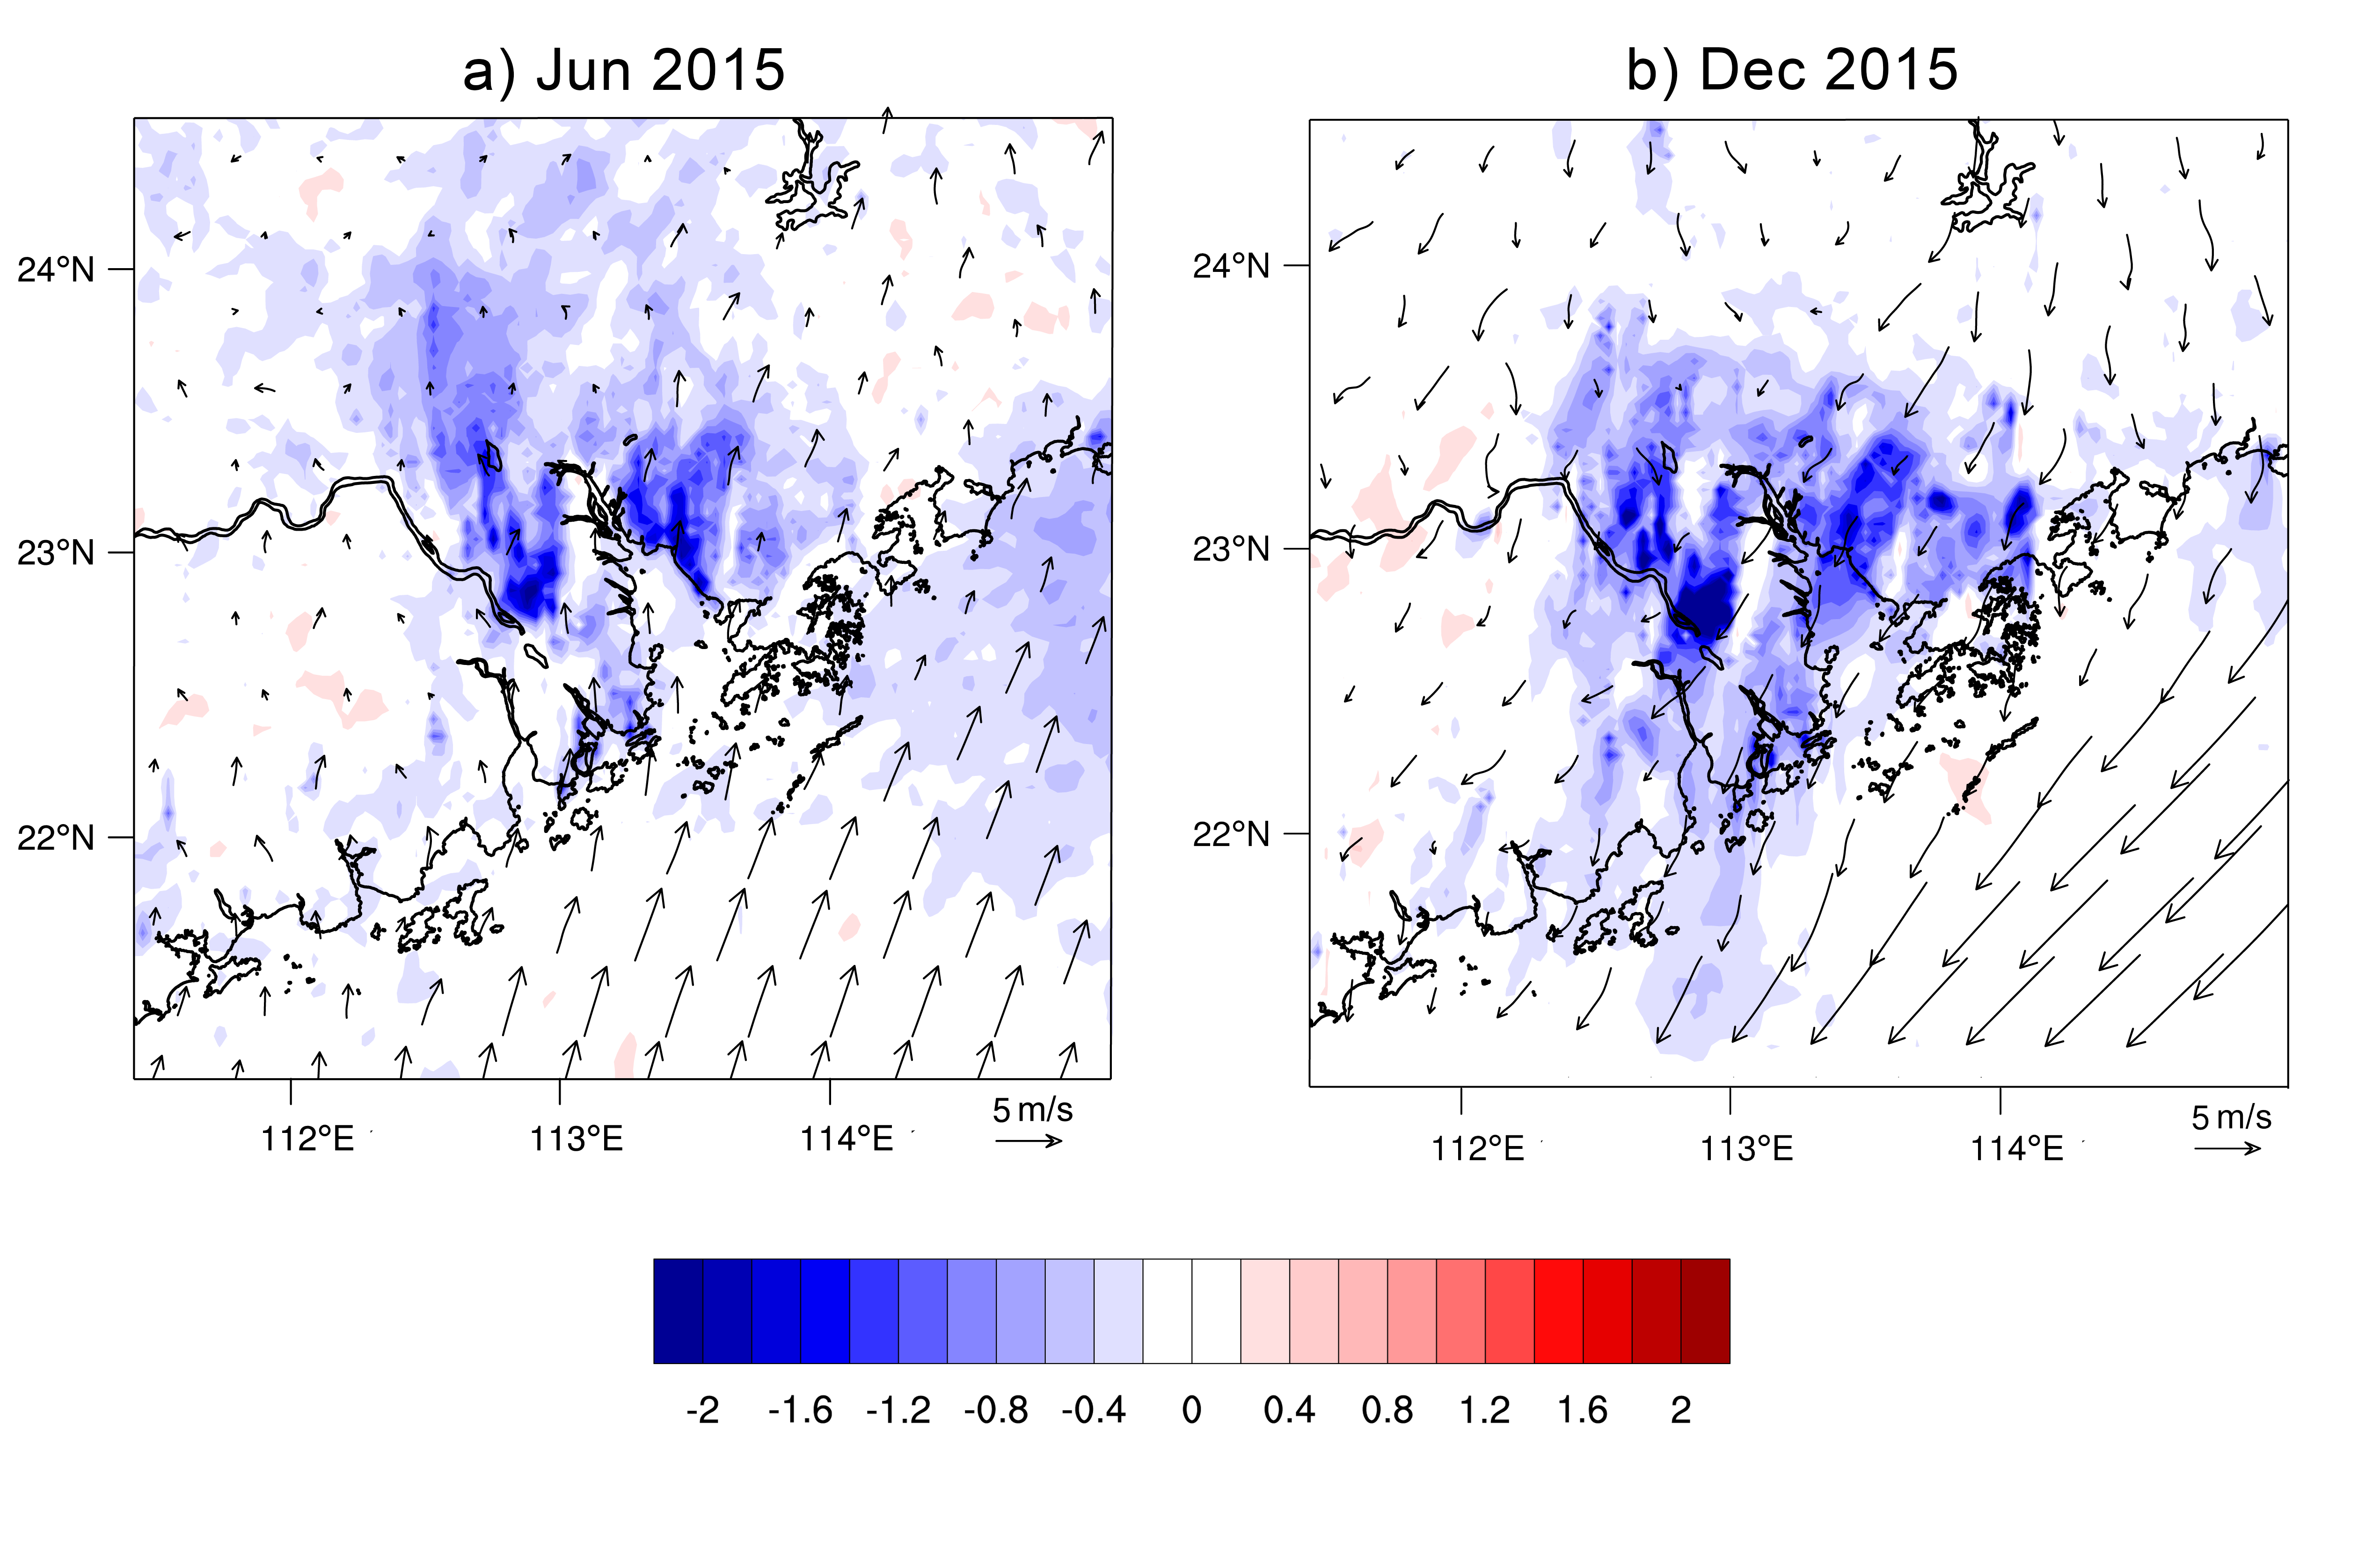
\includegraphics[width=0.9\textwidth]{城市化对地表风速的影响}
    \bicaption{ 城市化对地表风速的影响($m ~ s^{-1}$)。a)使用2015年6月气象场模拟结果,b)使用2015年12月气象场模拟结果,矢量箭头为对应时间背景风矢量。}{Impact of urbanization on surface wind speed (in $m ~ s^{-1}$). a)Model simulation using June 2015 meteorological fields, b)Model simulation using December 2015 meteorological fields, vectors are background wind vectors during corresponding periods.}
    \label{fig:urbanizationonwind}
\end{figure}

\begin{figure}[!htbp]
    \centering
    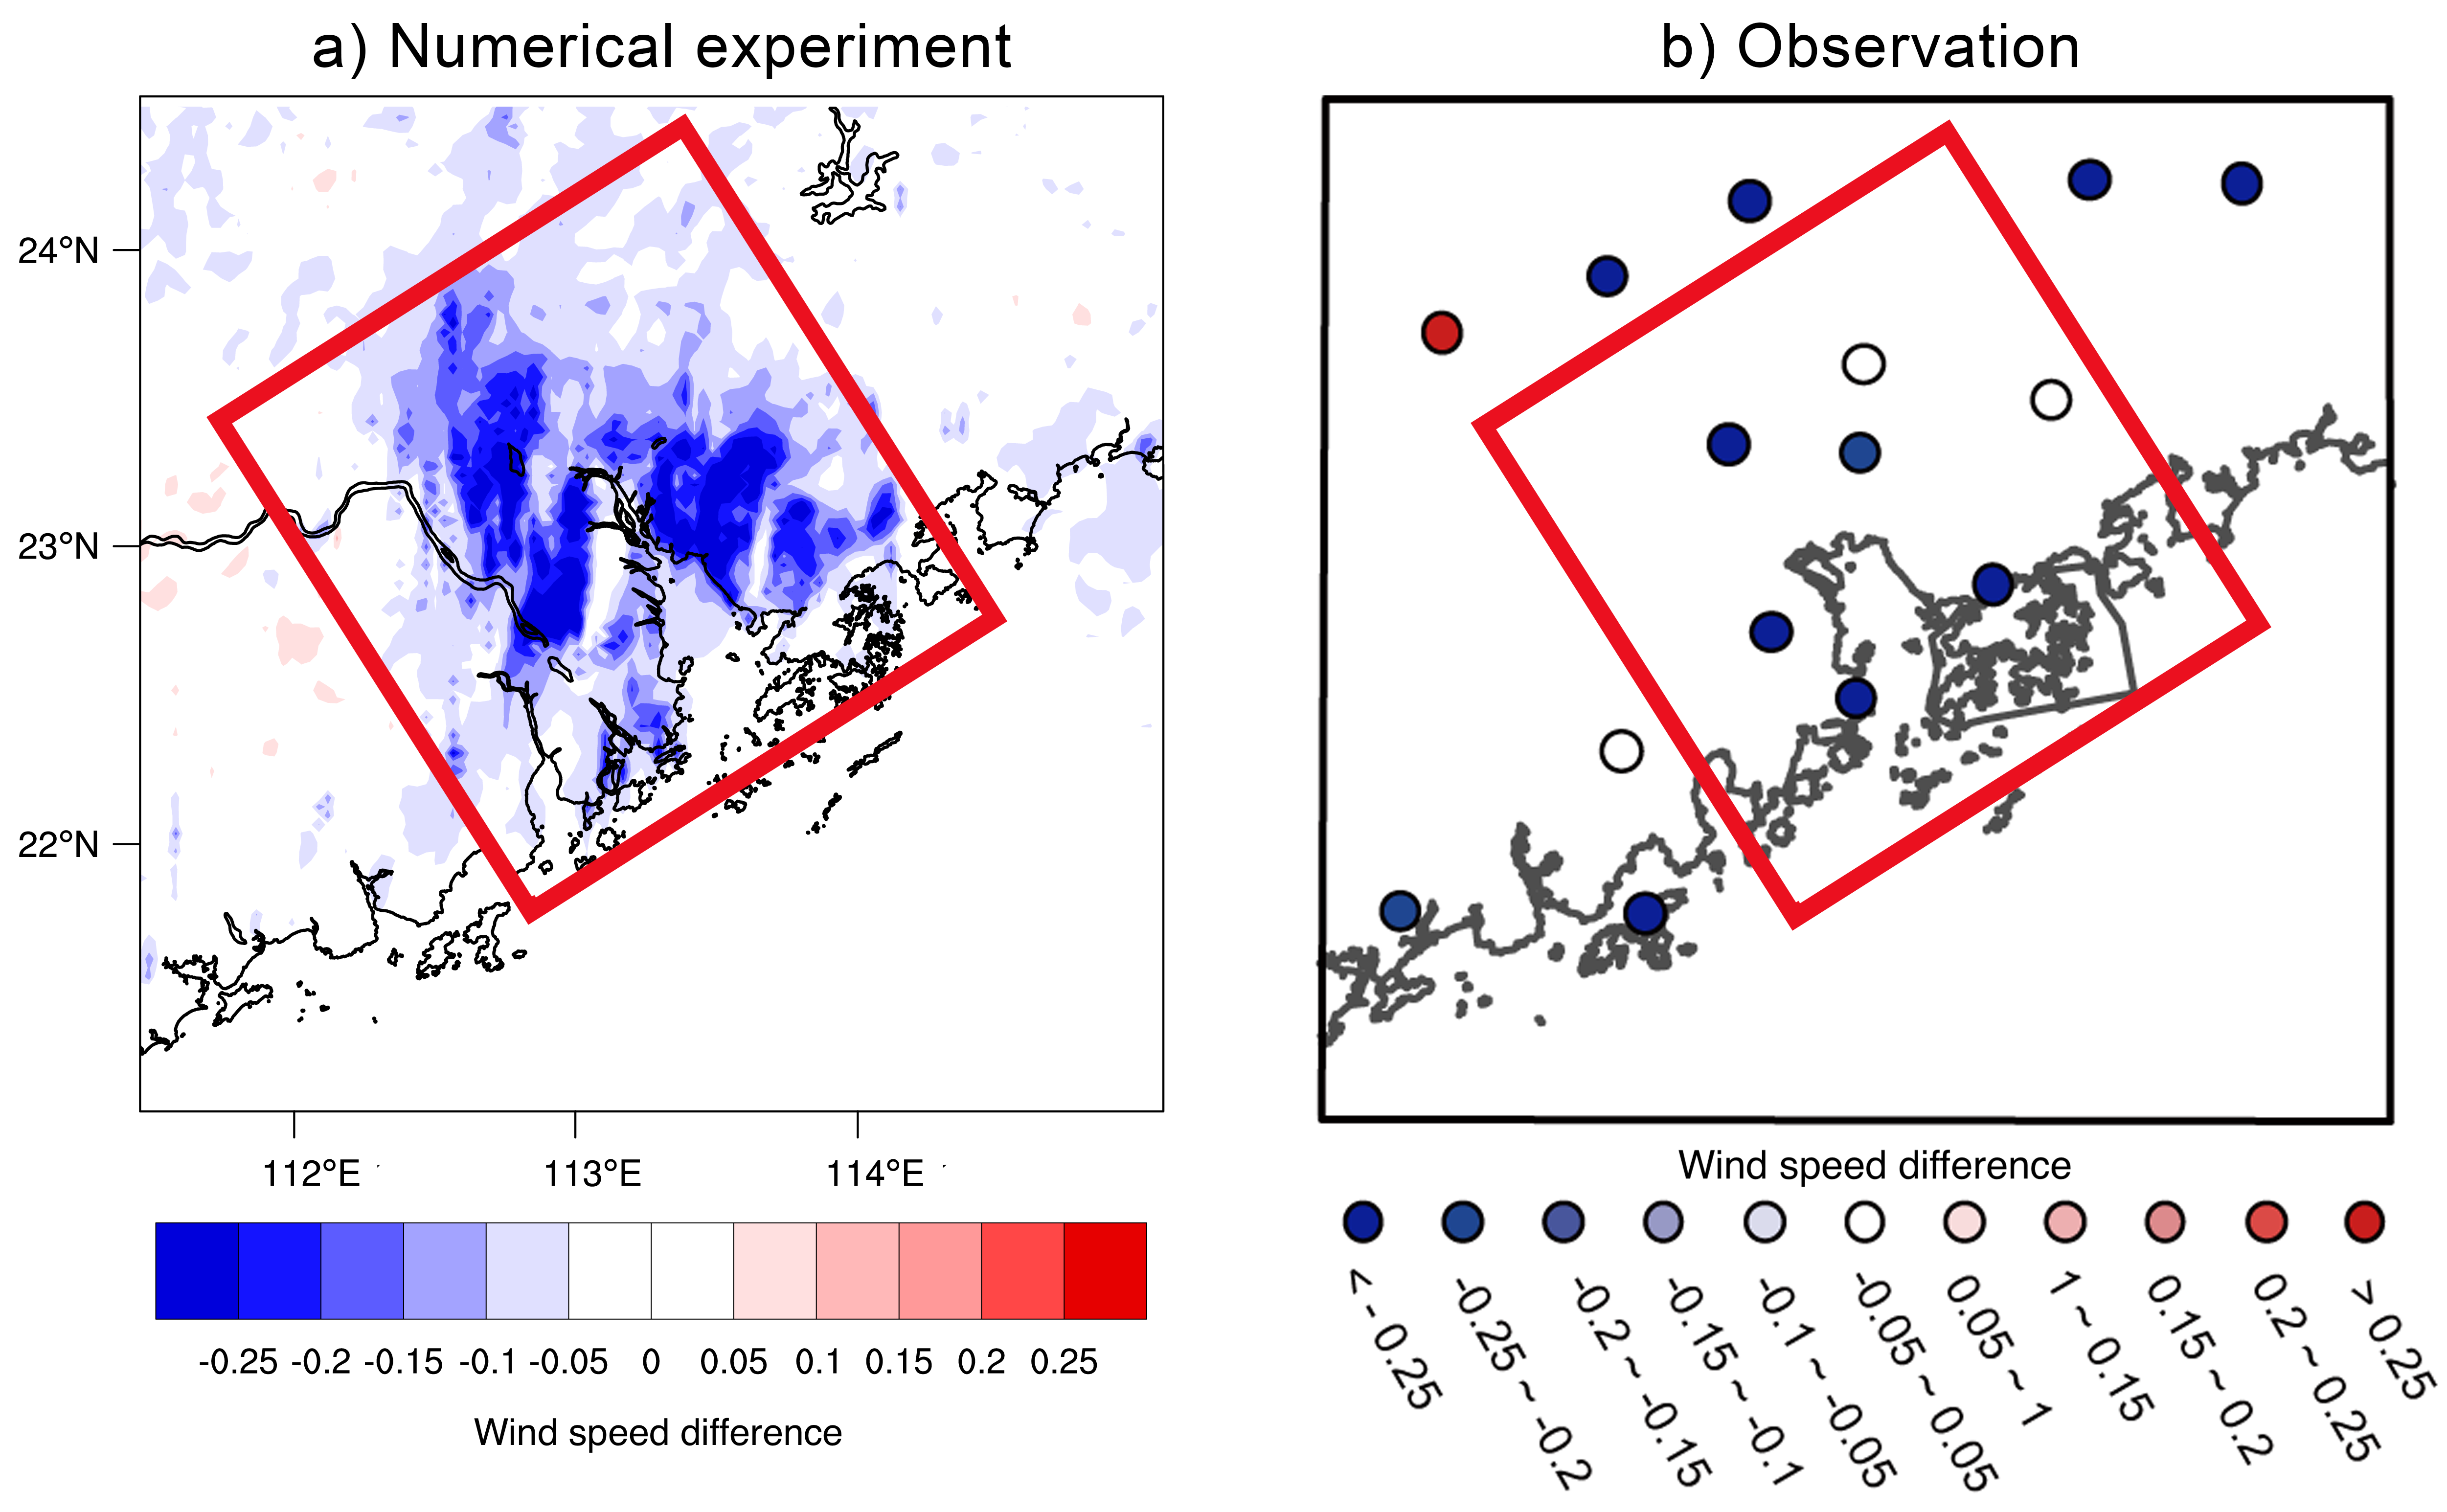
\includegraphics[width=0.9\textwidth]{珠江三角洲模拟结果与观测对比}
    \bicaption{ 珠江三角洲模拟与观测风速变化(变化率)。a)模拟结果,b)观测结果。}{Simulated and observed wind speed change in the Pearl River Delta (in $changing ~ rate$). a)Simulation, b)Observation.}
    \label{fig:wrfvsobs}
\end{figure}

\begin{figure}[!htbp]
    \centering
    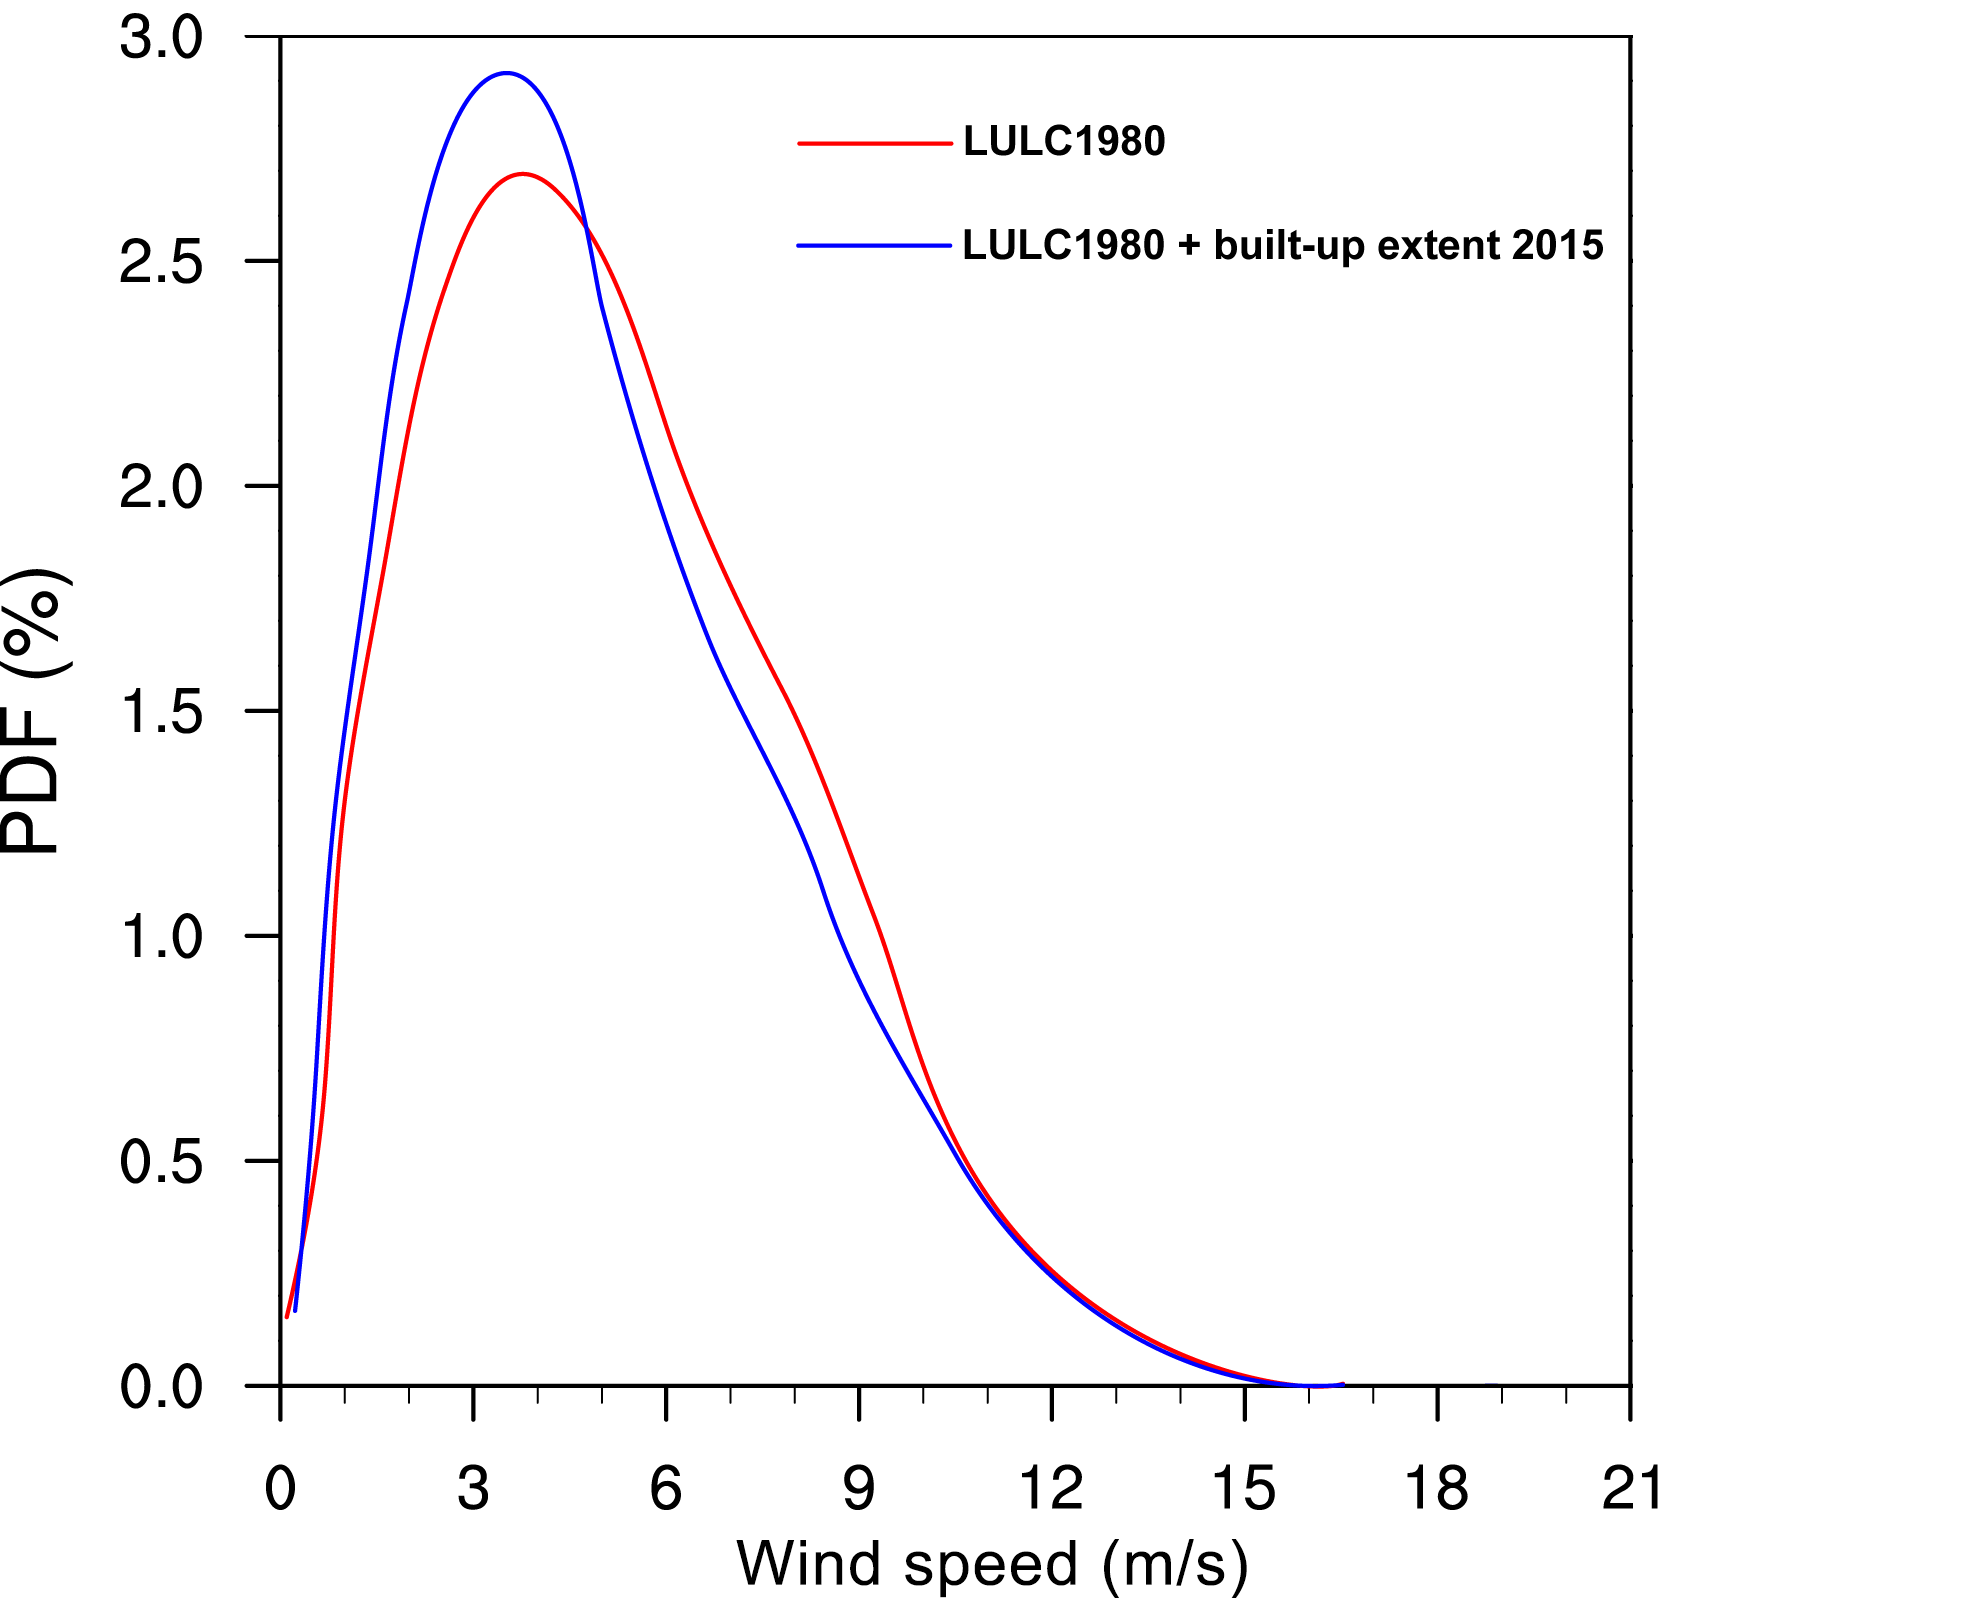
\includegraphics[width=0.5\textwidth]{城市化对风速概率密度分布的影响}
    \bicaption{ 珠江三角洲20世纪70年代末与2015年城市化状况下风速概率密度分布。红色(蓝色)实线为使用20世纪70年代末城市化状况(2015年城市化状况)的模拟结果。}{Probability distribution function of wind speed in the Pearl River Delta under the built-up condition in late 1970s and 2015. Red (Blue) line is the simulation result using built-up condition in late 1970s (2015).}
    \label{fig:windPDF}
\end{figure}

将模拟\ref{sim:1.2} 与模拟\ref{sim:1.1} 的模拟结果相减,得到城市建设面积变化对于地表风速的影响。发现相对20世纪70年代末,珠江三角洲在2015年城市化状况下风速显著偏小,城市群所在区域风速差可达 1 $m ~ s^{-1}$以上。同时,城市群下风向地区风速也表现出偏小,6月珠江三角洲盛行偏南风,城市群北部有风速偏小区域;12月珠江三角洲盛行偏北风,城市群南部有风速偏小区域(图 \ref{fig:urbanizationonwind})。将两个月模拟结果平均,并插值到6个观测站点(图 \ref{fig:wrfvsobs} b) 红框内),得到风速平均减小了11.6\%,相比之下,观测风速在1979-2016平均减小了33.4\%,由此可得城市化对于风速减小的贡献达到35\%(图 \ref{fig:wrfvsobs})。此外,城市化对于风速的影响主要体现在大风,2 $m ~ s^{-1}$以下风速变化很小(图 \ref{fig:windPDF})。

\section{植被变化的影响}

\subsection{基于NDVI和风速观测数据的统计学分析}

使用GIMMS NDVI 3g观测站点周围3 $ \times$ 3(\textasciitilde 25 $\times$ 25 $km$)北半球植被生长期(4-9月)平均计算得到1982-2015年NDVI趋势,发现亚洲和欧洲的大部分区域NDVI有显著增加,表明植被有明显增加,相比之下,北美洲NDVI无明显趋势(图 \ref{fig:NDVItrend})。将NDVI趋势与风速趋势对比,没有发现有明显的相关关系,原因可能是草地等低矮植被的变化对10 $m$风速无明显影响,而林地等高大植被变化才能够对10 $m$风速产生影响。选取林地覆盖面积超过90\%的芬兰,且其在2001-2016年间有超过95\%的植被变化来自林地变化(图 \ref{fig:Finlandvegetation}),发现NDVI趋势与风速趋势呈显著负相关(p < 0.05)(图 \ref{fig:FinlandwindvsNDVI}),表明植被(主要是林地)增加的区域风速趋向于减小。

\begin{figure}[!htbp]
    \centering
    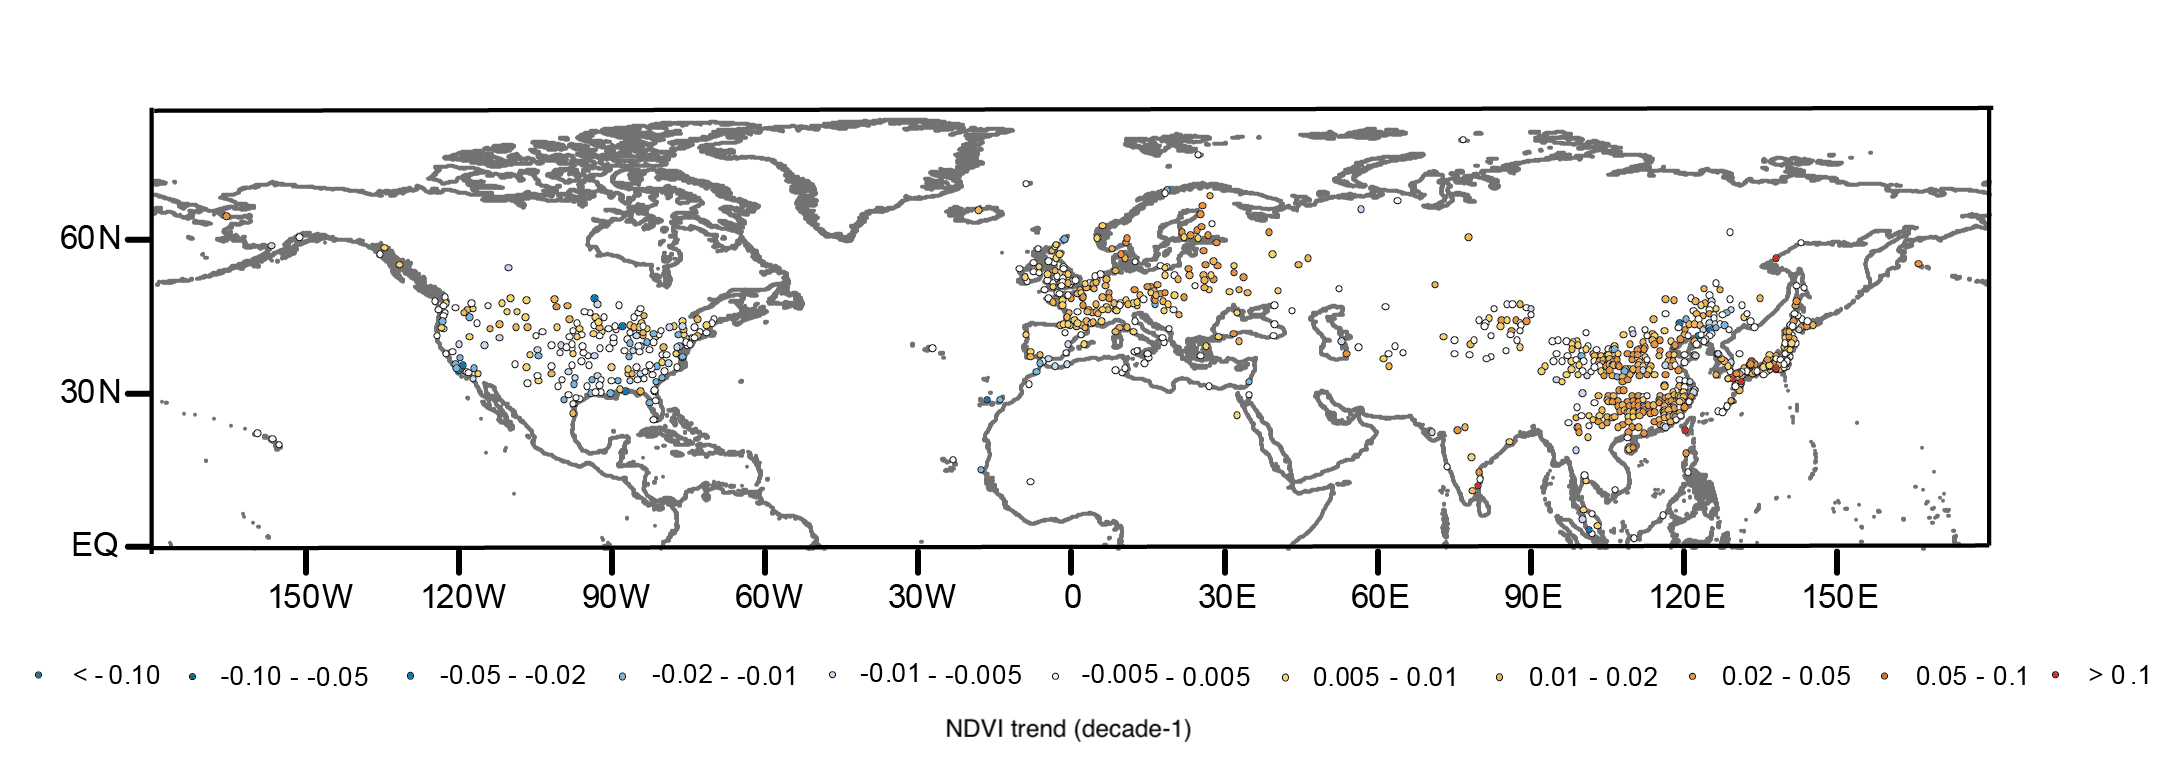
\includegraphics[width=1 \textwidth]{NDVI趋势}
    \bicaption{北半球植被生长季NDVI趋势( 每十年)}{Growing season NDVI trend over the Northern Hemisphere (in $decade^{-1}$).}
        \label{fig:NDVItrend}
\end{figure}

\begin{figure}[!htbp]
    \centering
    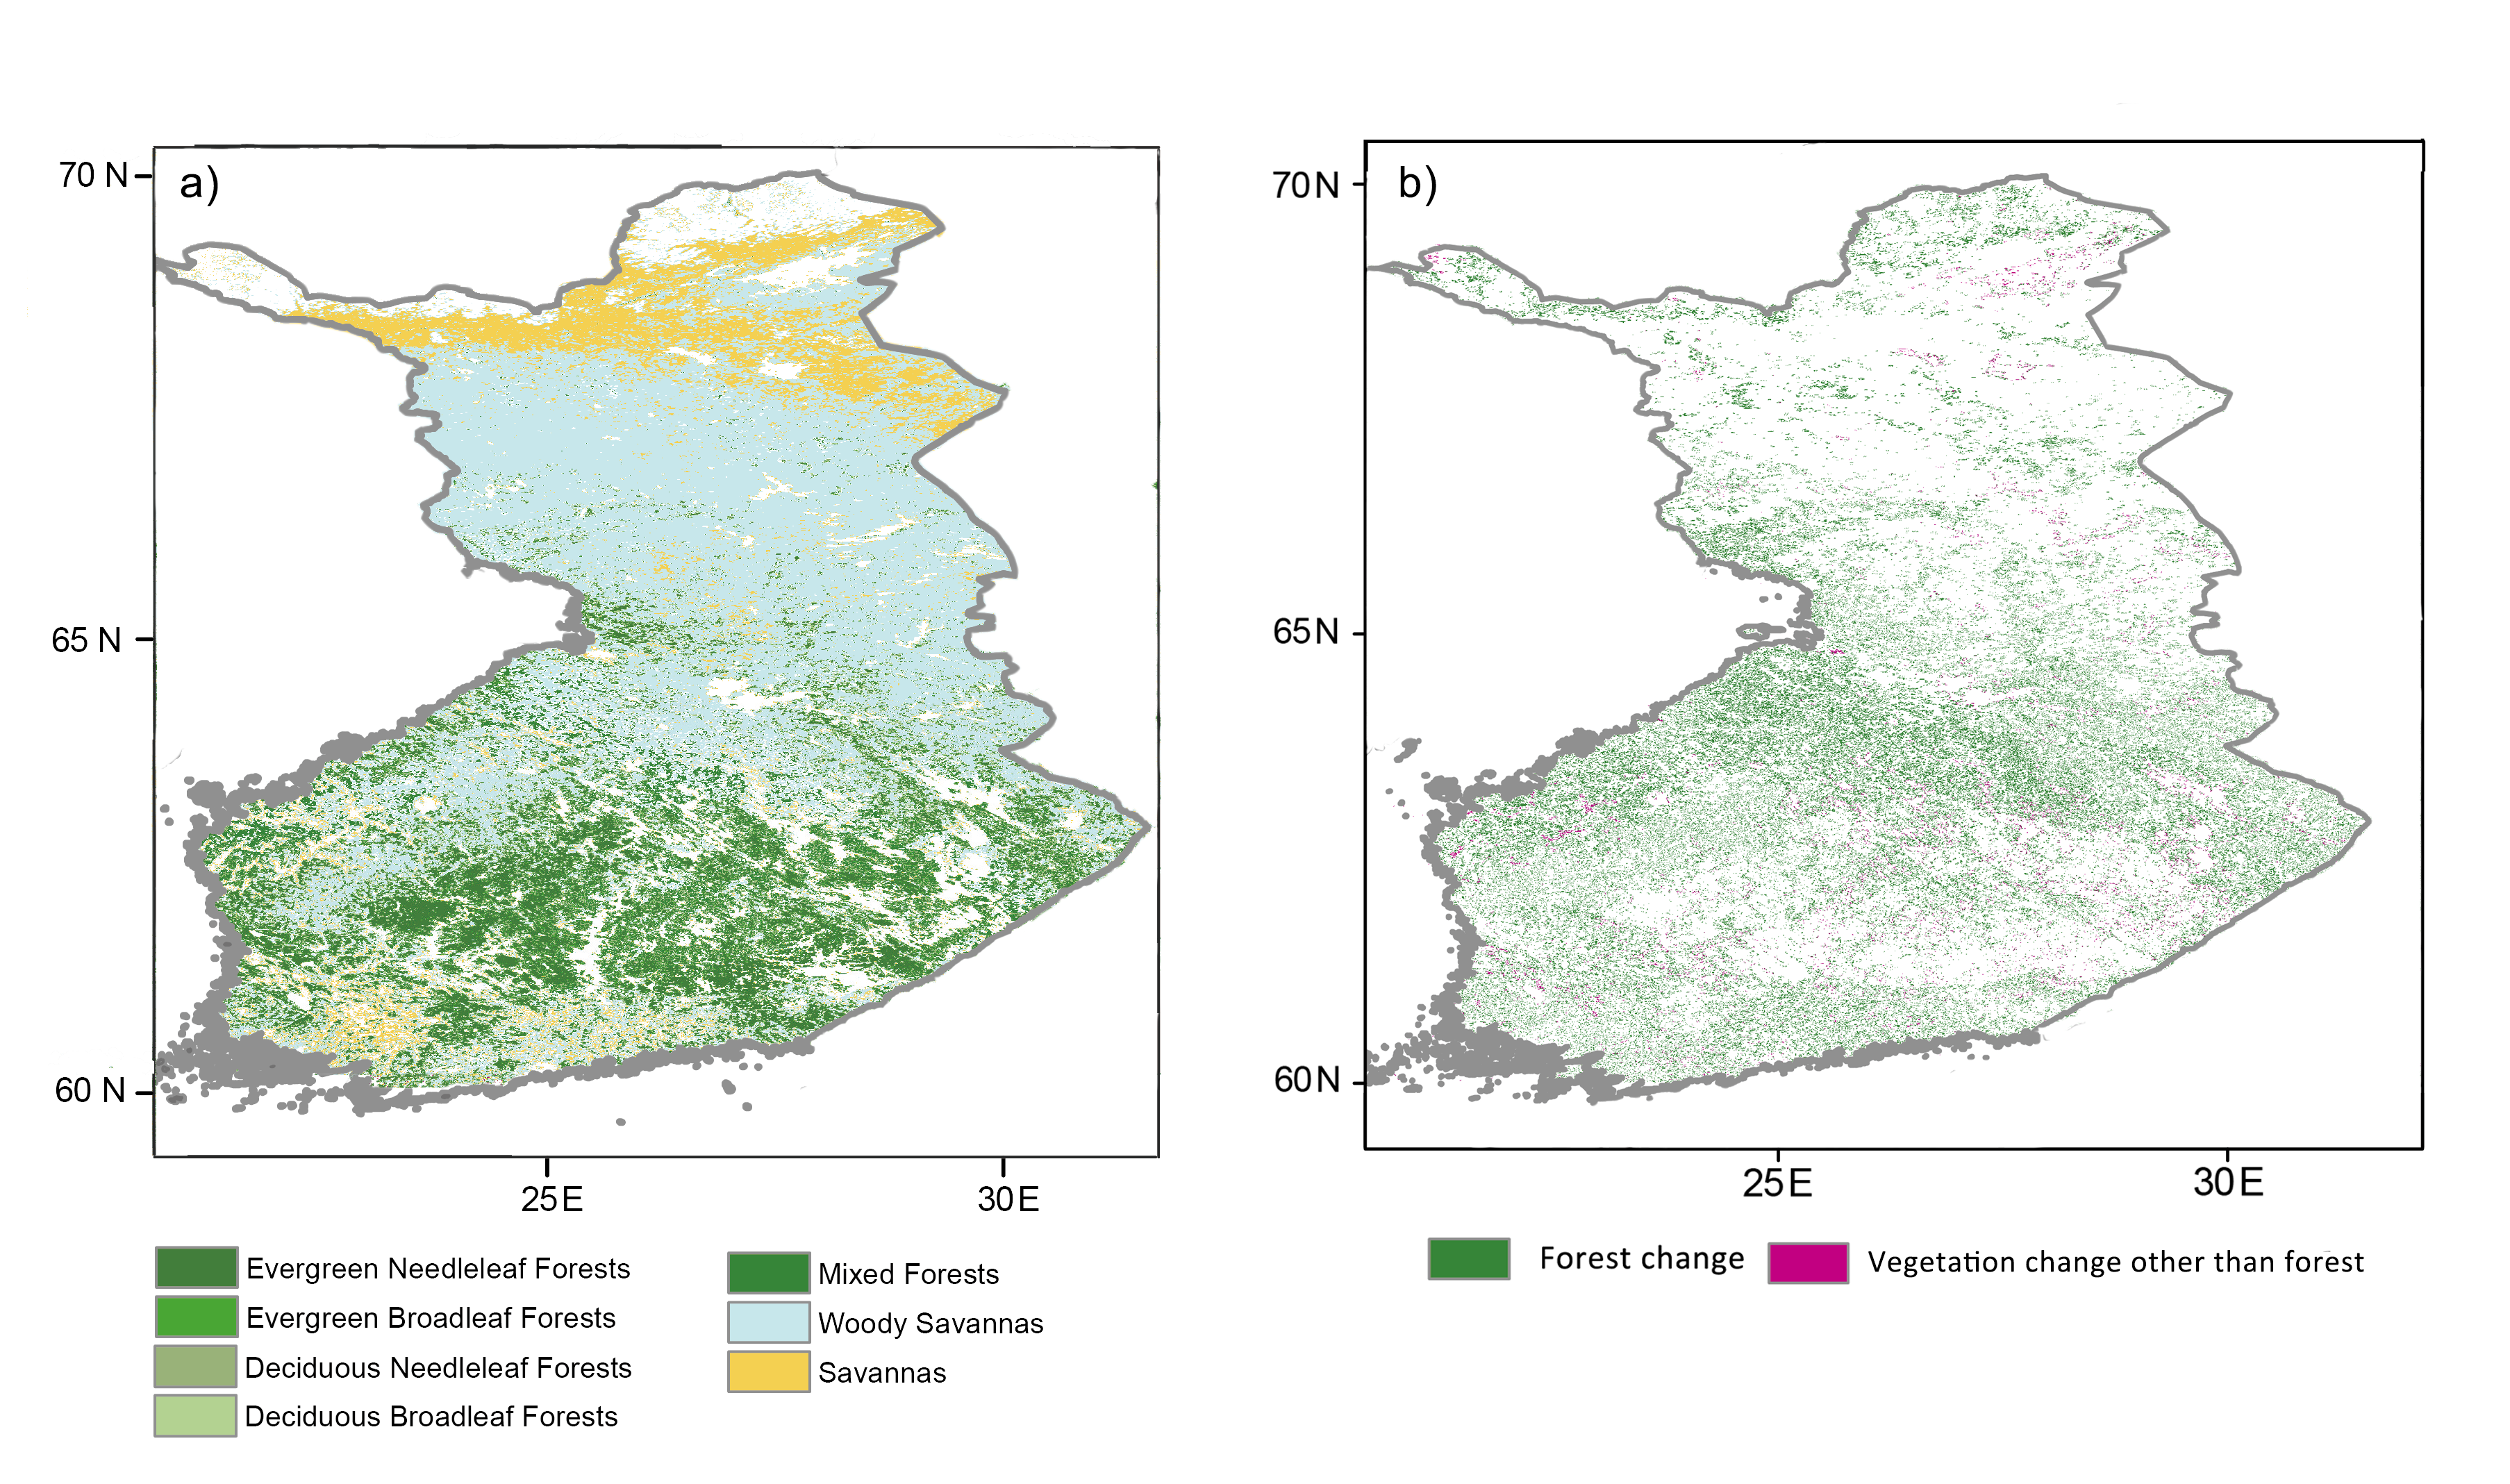
\includegraphics[width=0.9 \textwidth]{芬兰植被分布与变化}
    \bicaption{芬兰植被分布与变化。a)芬兰2001年林地分布,b)芬兰2016相对2001植被变化,绿色为林地变化,红色为除林地外其他植被变化。}{Spatial distribution and temporal change of vegetation in Finland. a)Spatial distribution in 2000, b)Change from 2001 to 2016, green denotes woodland change, red denotes vegetation change other than woodland.}
        \label{fig:Finlandvegetation}
\end{figure}

\begin{figure}[!t]
    \centering
    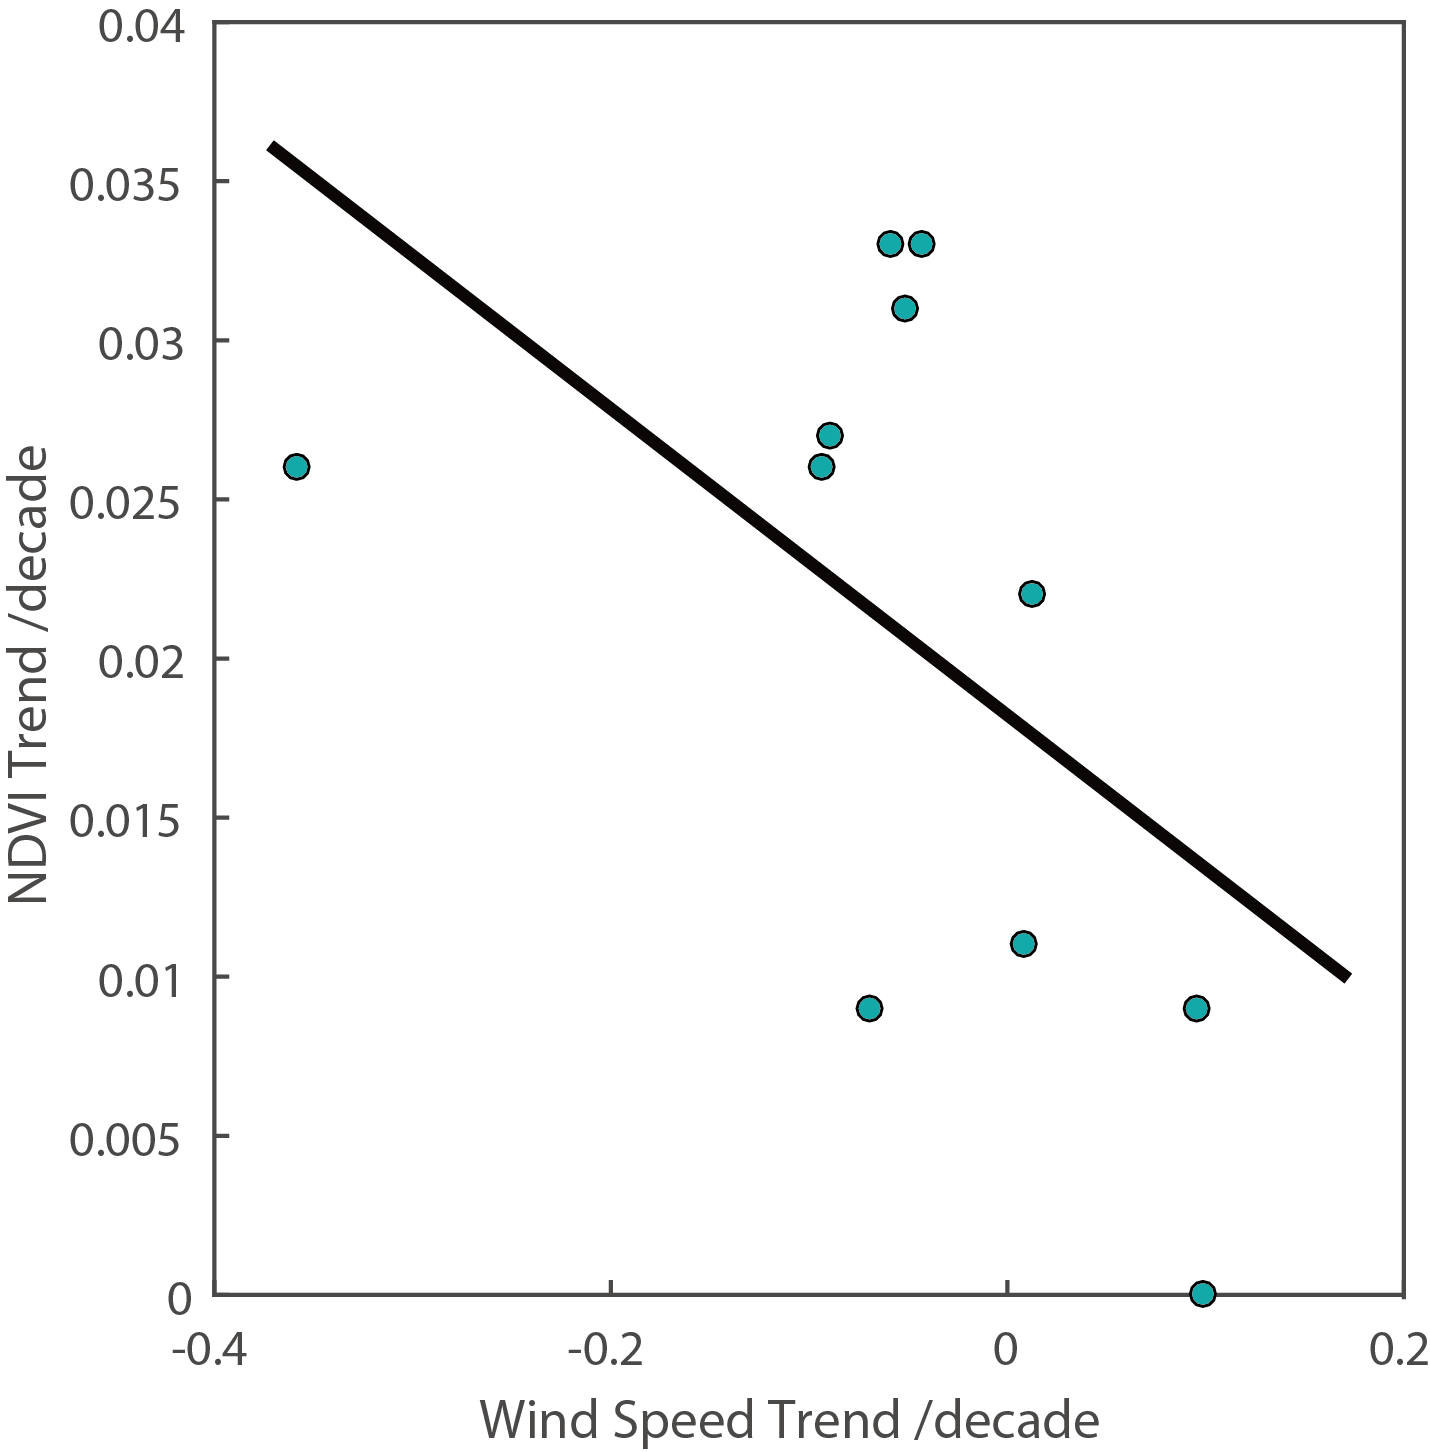
\includegraphics[width=0.5 \textwidth]{ndvi与风速变化}
    \bicaption{芬兰站点风速趋势与附近NDVI趋势}{Wind speed trend and NDVI trend nearby in Finland.}
        \label{fig:FinlandwindvsNDVI}
\end{figure}

\subsection{数值试验}

使用WRF-ARW 4.0进行数值试验进一步验证植被与风速变化的关系,选择芬兰植被变化更为明显同时也是大部分观测站点所在的南芬兰作为模拟区域(图 \ref{fig:Finlandstations})。将模式设置为四层双向嵌套,空间分辨率分别为30 $km$、10 $km$、3.3 $km$和1.1 $km$(图 \ref{fig:Finmodeldomain}),垂直包含40个层次,其中边界层内(1 $km$高度以下)10个层次;时间步长为100 $s$;微物理参数化方案为WRF Single-Moment 6-class scheme \citep{hong2006the};积云参数化方案为Grell 3D \citep{grell1993prognostic, grell2002a},在较高分辨率的两层网格关闭积云参数化;云量使用Xu-Randall method \citep{xu1996a};长波辐射参数化方案为RRTM scheme \citep{mlawer1997radiative},短波辐射参数化方案为Dudhia scheme \citep{dudhia1989numerical};边界层采用BouLac PBL \citep{bougeault1989parameterization},陆面模式选择Noah-MP \citep{niu2011the}。

\begin{figure}[!hbtp]
    \centering
    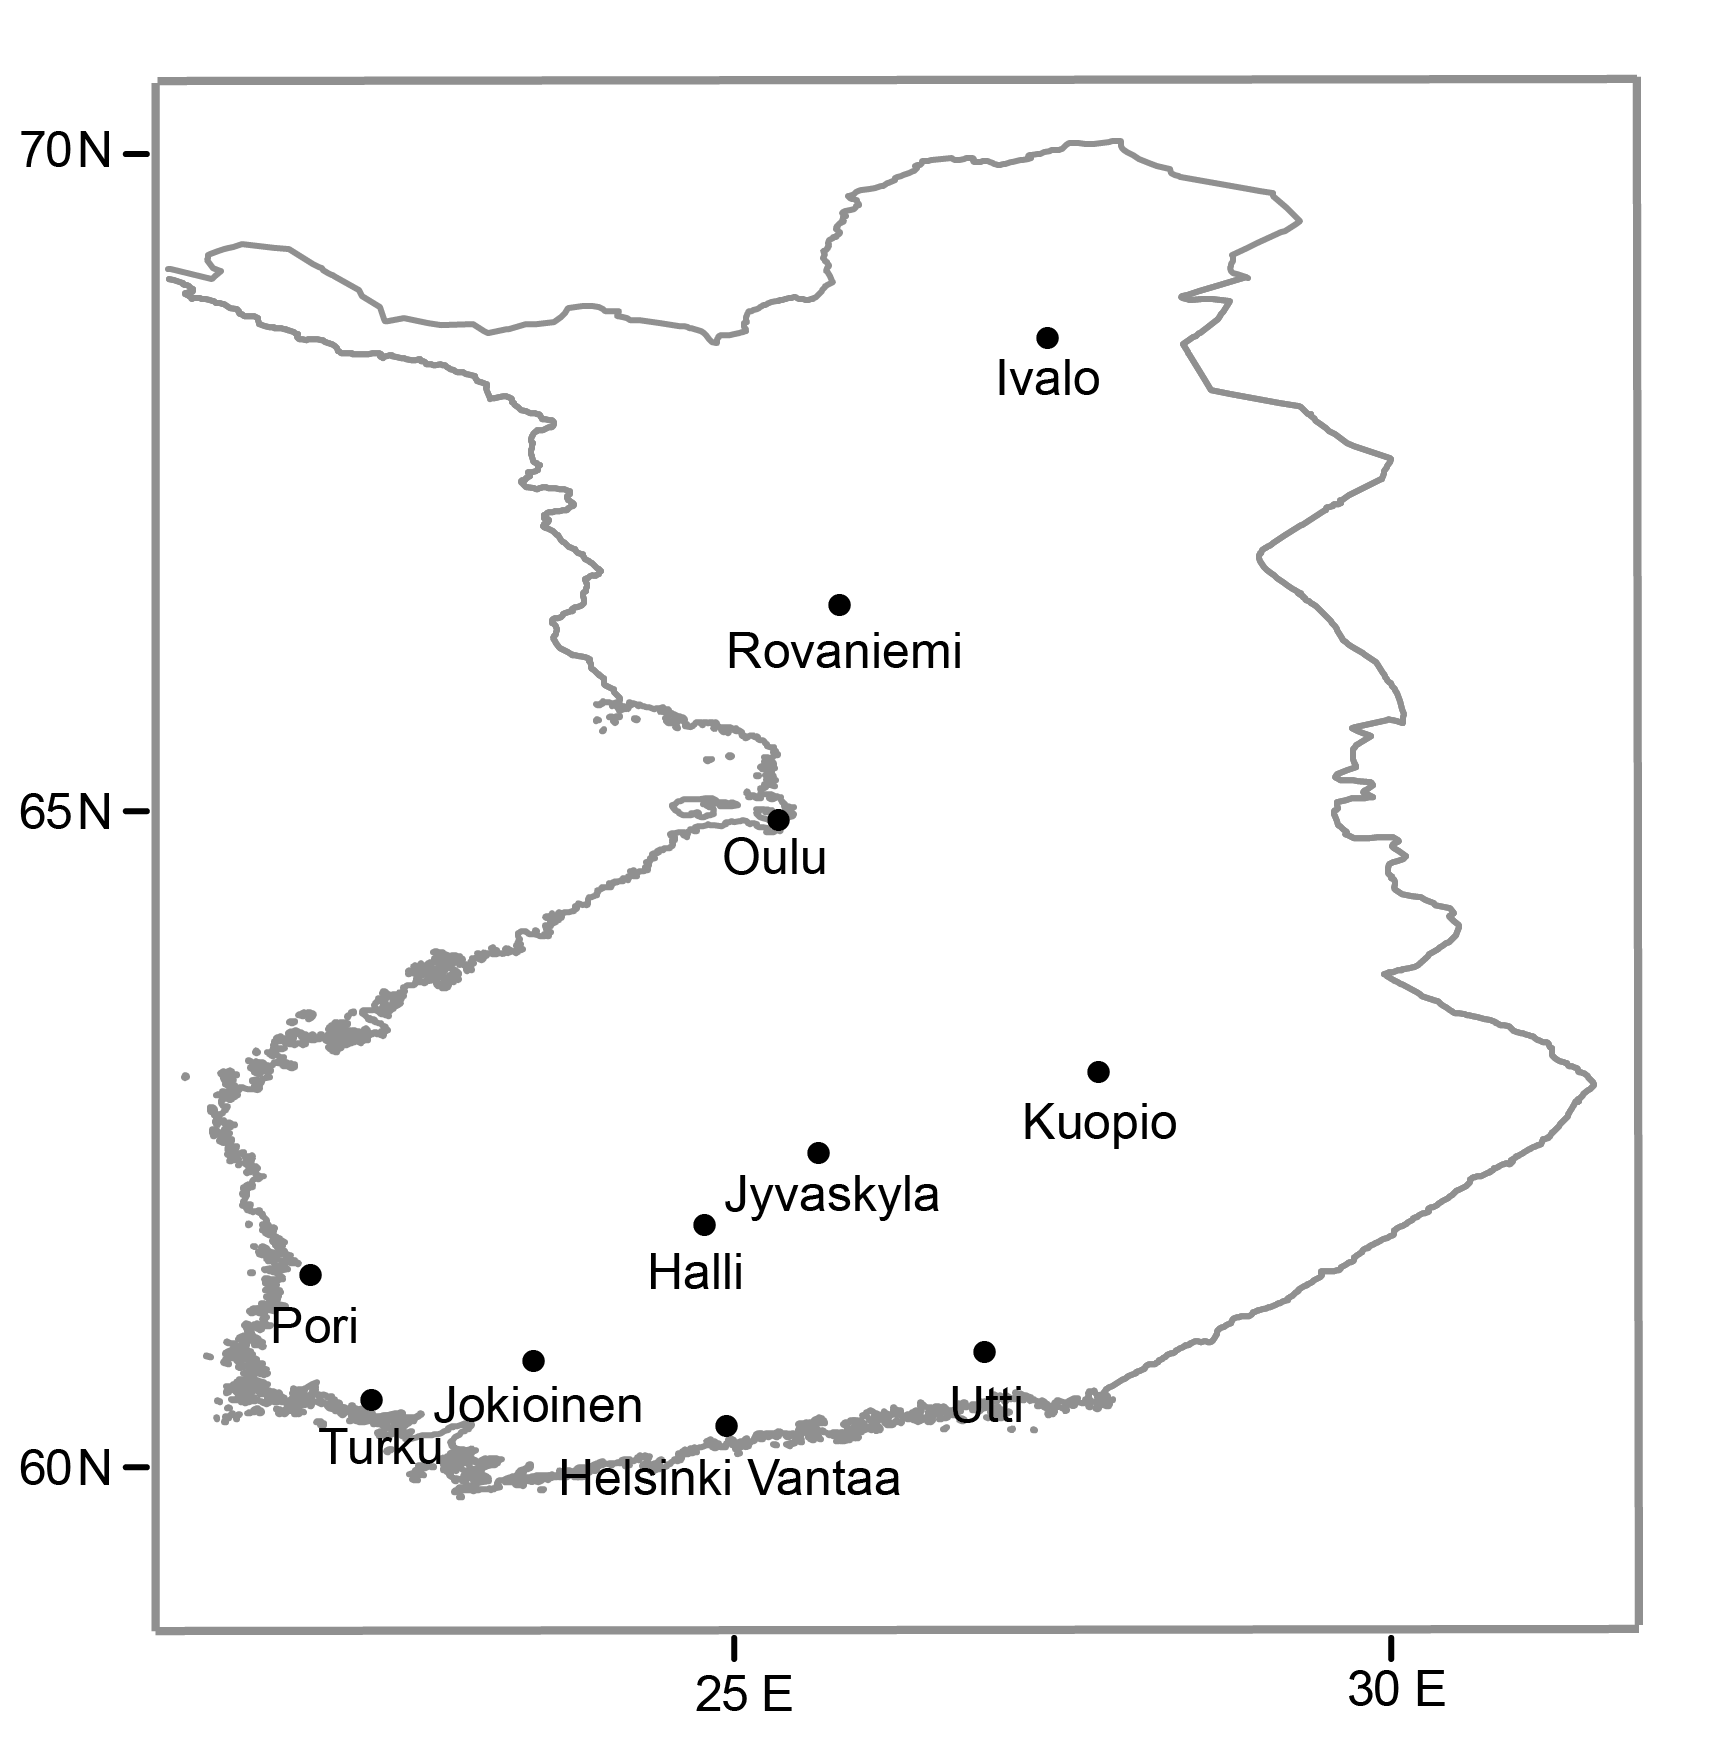
\includegraphics[width=0.6 \textwidth]{芬兰站点分布}
    \bicaption{芬兰站点分布}{Locations of observation stations in Finland.}
        \label{fig:Finlandstations}
\end{figure}

\begin{figure}[!hbtp]
    \centering
    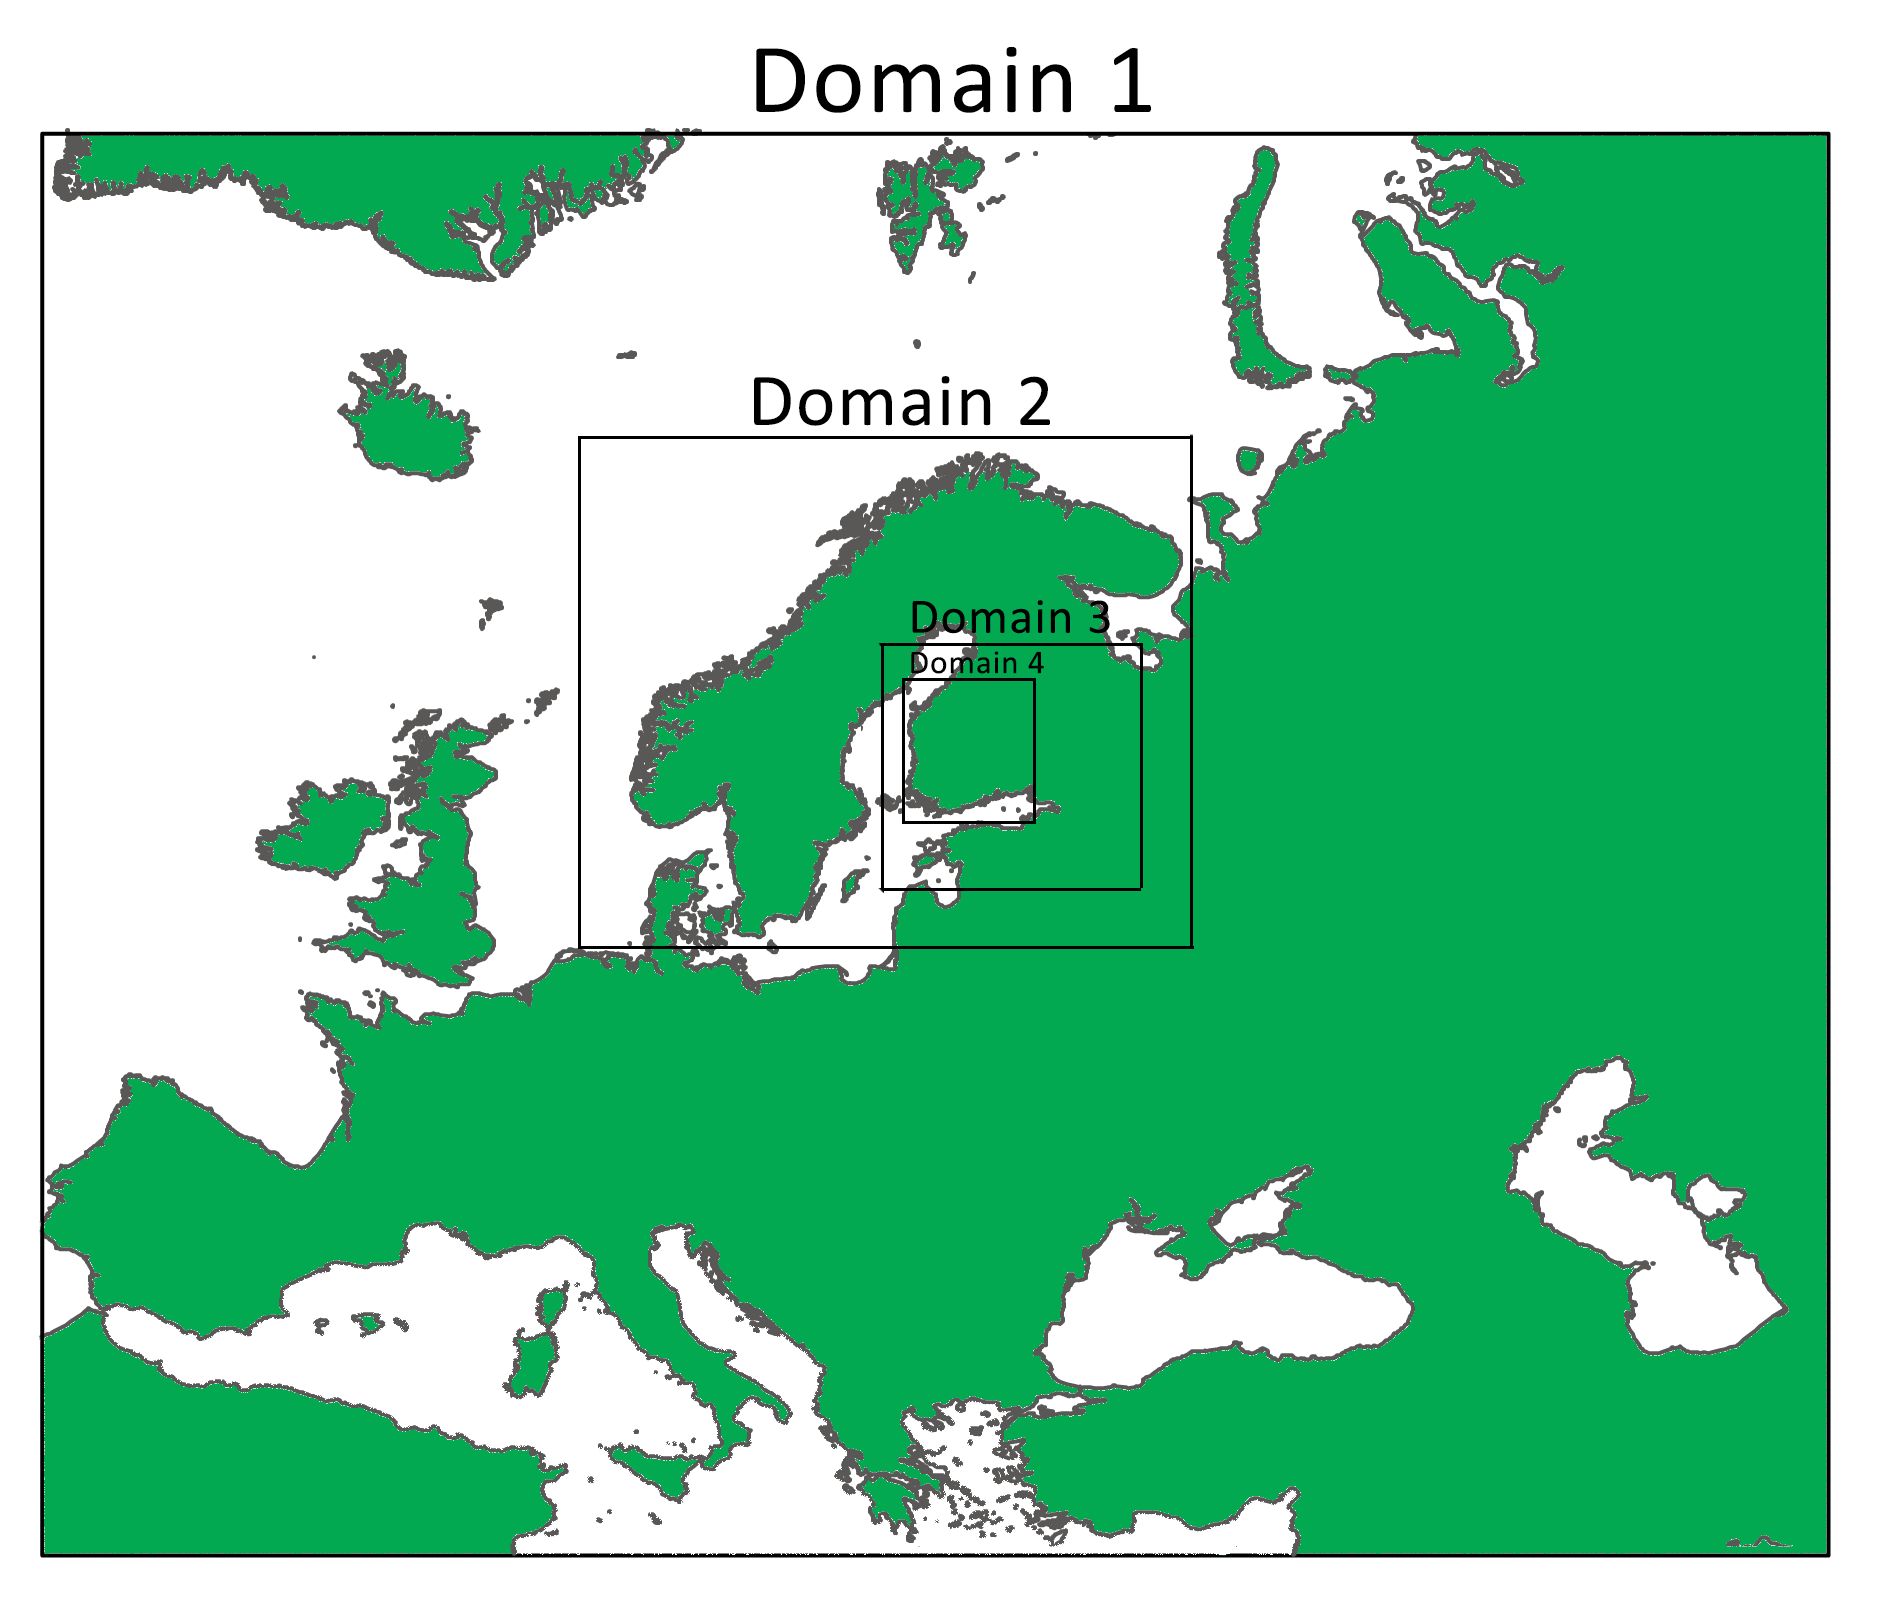
\includegraphics[width=0.8 \textwidth]{模拟区域2}
    \bicaption{模拟区域}{Model simulation domains}
        \label{fig:Finmodeldomain}
\end{figure}

采用以上模式设置进行两组模拟,分别为:

\begin{enumerate}

\item \label{sim:2.1} 以南芬兰地区2001年土地利用类型(MODIS12Q1)作为下边界条件进行模拟。

\item \label{sim:2.2} 以南芬兰地区2001年土地利用类型叠加2016相对2001年南芬兰地区林地变化作为下边界条件进行模拟。

\end{enumerate}

对以上两组模拟,气象场采用FNL2001年1月和2001年6月(分别代表植被非生长季节和生长季节)1$\times$ 1度6小时分辨率物理量场。模式积分过程分为4段,每段约7天。

使用模拟\ref{sim:2.1}进行模式性能评估,南芬兰地区观测站信息参见表 \ref{tab:Finlandstationinfo},表中除Oulu、Rovaniemi、Ivalo外,其余站点均分布在南芬兰。对比模拟与观测结果,与本章\ref{sec:urbanimpact}节类似,模拟风速大于观测风速,但二者相关系数较高,表明模拟能够较好的抓住风速随时间的变化,RMSD也较低,总体来看模式模拟效果良好。

\begin{table}[!htbp]
    \bicaption{南芬兰站点信息及模式性能评估结果}{Description of observation stations in the southern Finland and model validation results}
    \label{tab:Finlandstationinfo}
    \centering
    \small% fontsize
    \setlength{\tabcolsep}{5 pt}% column separation
    \renewcommand{\arraystretch}{1.0}%row space 
    \begin{tabular}{lccccccc}
        \hline
        站名 & 站号 & 纬度 & 经度 & 海拔($m$)&  \multicolumn{3}{c}{10 $m$ 风速} \\
         & & & & & 均值($m ~ s^{-1}$)$^*$ &  相关系数 $^ {**}$ & RMSD \\
        %\cline{2-9}% partial hline from column i to column j
        \hline
        Pori & 29520 & 61.47 & 21.8 & 13.4 & 5.4(-1.4) & \textbf{0.38} & 1.35 \\
        Turku & 29720 & 60.52 & 22.27 & 49.1 & 5.0(-1.7) & 0.26 & 1.57 \\
        Jokioinen & 29630 & 60.82 & 23.50 & 103.0 & 4.8(-1.8) & 0.04 & 1.41 \\
        Helsinki Vantaa & 29740 & 60.32 & 24.97 & 54.6 & 4.5(-0.6) & \textbf{0.34} & 1.27 \\
        Halli & 29450 & 61.80 & 24.80 & 146.0 & 4.6(-1.5) & \textbf{0.36} & 1.34 \\
        Jyvaskyla & 29350 & 62.40 & 25.67 & 139.9 & 4.5(-1.1) & 0.27 & 1.43 \\
        Utti & 29660 & 60.88 & 26.93 & 103.3 & 4.0(-0.8) & \textbf{0.34} & 1.33 \\
        Kuopio & 29170 & 63.02 & 27.80 & 98.5 & 5.2(-1.9) & \textbf{0.42} & 0.99 \\ 
        \hline
    \end{tabular}
    
     \vspace*{3ex}  
      
    \begin{minipage}{1\textwidth}% choose width suitably
    注:$^*$ 括号外数值为模拟结果,括号内为观测减去模拟。\\ 
    $^{**}$ 加粗的数值代表 p < 0.01。r = 0.33 对应 p = 0.01, r = 0.25 对应 p = 0.05。
    \end{minipage}
\end{table}


将模拟\ref{sim:2.2}与\ref{sim:2.1}相减,得到林地变化对于风速的影响。由林地变化造成的对风速影响中,主要的作用是风速减小(图 \ref{fig:woodlandonwind}),考虑到林地变化中的超过70\%是增加(图(芬兰林地变化)),得到这种模拟结果非常合理。1月林地变化对于风速变化的影响明显小于7月,因而1月很多落叶林地变得光秃,对风速的影响变小。将两个月的模拟结果平均,计算归一化风速变化,插值到观测站点,得到南芬兰8个站点林地对风速影响平均为-2.5\%。假设林地变化与风速变化满足线性关系(即 $\Delta(woodland ~ area) = \alpha \Delta(wind ~ speed)$),并以NDVI代替林地变化,得到1979-2016林地变化对风速的影响在8个站点平均为-5.1\%,而观测风速的变化为-5.8\%,即林地变化可以解释南芬兰风速变化的87\%。

\begin{figure}[!t]
    \centering
    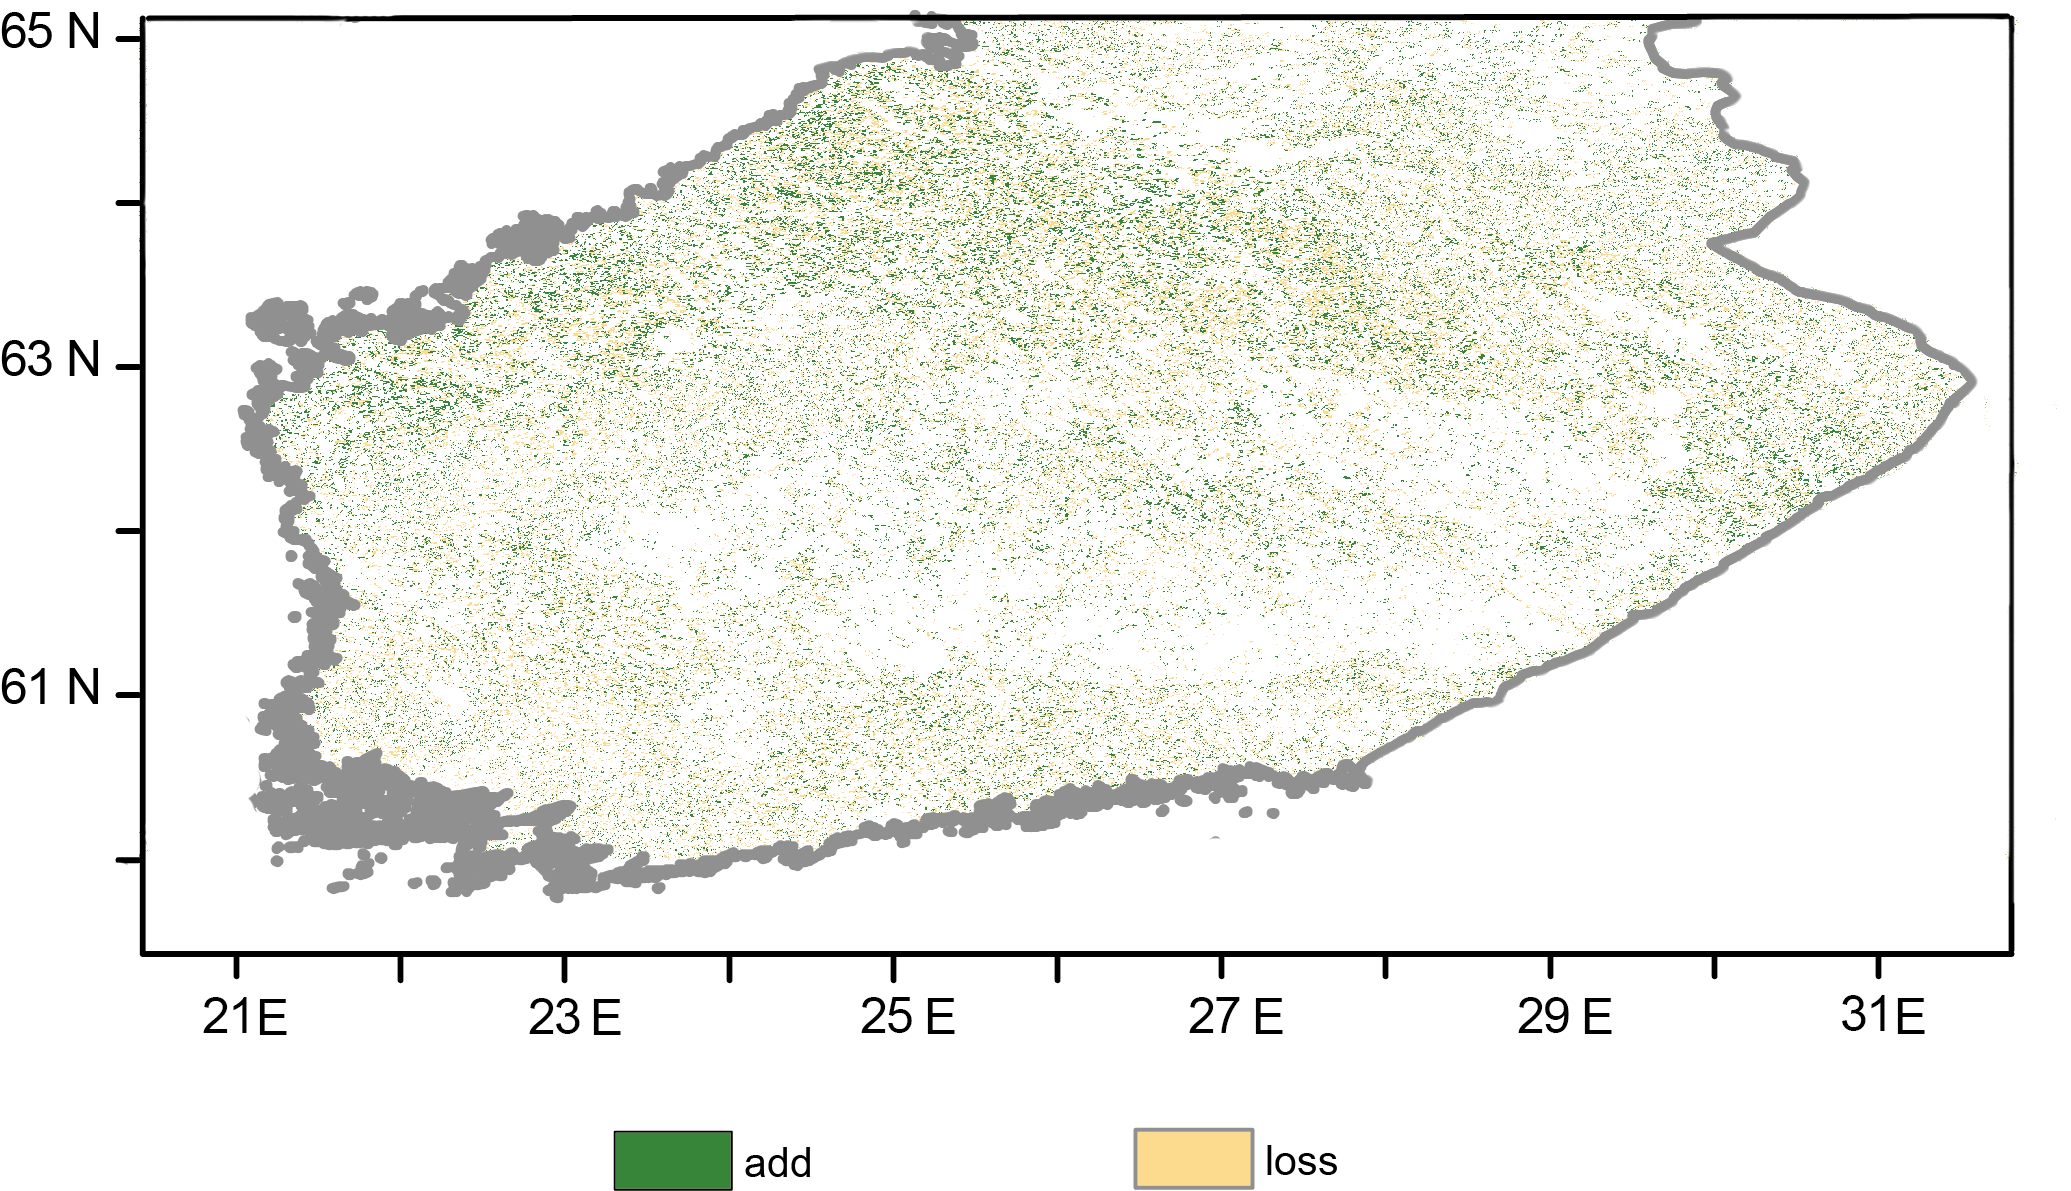
\includegraphics[width=0.6 \textwidth]{芬兰林地变化}
    \bicaption{南芬兰林地变化。绿色为增加,黄色为减少。}{Woodland change in southern Finland. Green color denotes add, yellow denotes lose.}
        \label{fig:Finlandwoodlandchange}
\end{figure}

\begin{figure}[!b]
    \centering
    \includegraphics[width=1 \textwidth]{林地变化对地表风速的影响}
    \bicaption{林地变化对地表风速的影响。a)使用2001年1月气象场模拟结果($ m ~ s^{-1}$),b)使用2001年7月气象场模拟结果($ m ~ s^{-1}$),c)a和b模拟结果平均归一化的结果。}{Impact of woodland change on surface wind speed. a)Simulation with January 2001 meteorological fields (in $ m ~ s^{-1}$), b)Simulation with July 2001 meteorological fields (in $ m ~ s^{-1}$), c)Normalized value of a) and b) averaged.}
        \label{fig:woodlandonwind}
\end{figure}

\section{大气稳定度变化的影响}

使用HadGHCND地表日最高气温和HadAT 850 $hPa$气温的差值估计地表至850 $hPa$日间垂直温度递减率,因为缺乏对应的对人为误差进行调整过的850 $hPa$位势高度观测数据,计算时假设两层之间的高度变化可以忽略,这会对计算结果产生一定的不确定性。结果发现北美洲日间边界层垂直温度递减率有普遍减小,表明北美洲日间地表温度增加慢于850 $hPa$(约为边界层顶高度),这会使得边界层内稳定度增加,湍流活动减弱,高层动量难以传递到地表附近。这也一定程度上解释了为何北美洲对流层低层风速显著增加而地表风速显著减小。欧洲有效数据较少,大部分格点日间垂直温度递减率增加,表明地表日间增温快于对流层底层。亚洲的情况与欧洲类似,这种情况下有利于边界层内湍流活动发展,高层动量更容易传递到地表附近(图 \ref{fig:lapserate})。

\begin{figure}[!htbp]
    \centering
    \includegraphics[width=1 \textwidth]{近地层温度垂直递减率趋势}
    \bicaption{近地层垂直温度递减率趋势( 每十年)}{Near surface lapse rate trend (in $decade^{-1})$}
        \label{fig:lapserate}
\end{figure}

\section{本章小结}

本章从城市化,植被变化和大气稳定度变化三个方面分析了大气运动阻力变化对于陆地地表风速长期变化的影响,得到以下结论:

\begin{enumerate}

\item 近30多年来全球特别是亚洲城市化进程迅猛,城市化速度与风速趋势呈显著负相关关系,表明城市化进程是地表风速减小的重要原因,模式试验结果表明珠江三角洲城市变化可以解释1979年来观测风速减小的35\%。

\item 近30多年来NDVI在北半球普遍呈增长趋势,表明植被普遍增加,但其与风速变化并没有很好的相关关系,原因可能是草地等低矮植被对10 $m$风速难以产生显著影响。在植被变化由林地变化主导的芬兰发现NDVI与风速趋势呈显著负相关,模式试验结果表明南芬兰林地变化可以解释1979年以来观测风速减小的87\%。

\item 北美日间垂直温度递减率普遍呈负趋势,预示着湍流活动减弱,高层动量难以向地表附近传递,这也解释了为何北美自由大气风速和地表风速趋势呈反向变化。欧洲和亚洲日间垂直温度递减率大部分呈现正趋势,预示湍流活动增强,高层动量更容易向地表附近传递。

\end{enumerate}


% template
%\input{Tex/Chap_Intro}
%\input{Tex/Chap_Guide}
%---------------------------------------------------------------------------%
% main content
%-
%-> Appendix
%-
\cleardoublepage%
\appendix% initialize the environment
\input{Tex/Appendix}% appendix content
%-
%-> Backmatter: bibliography, glossary, index
%-
\backmatter% initialize the environment
\intotoc*{\cleardoublepage}{\bibname}% add link to toc
\bibliography{Biblio/ref}% bibliography
%---------------------------------------------------------------------------%
%->> Backmatter
%---------------------------------------------------------------------------%
\chapter{作者简历及攻读学位期间发表的学术论文与研究成果}


\section*{作者简历}

2018年9月 - 2019年9月~普渡大学地球、大气与行星科学系~联合培养

2014年9月至今~中国科学院大气物理研究所~气象学~硕博连读

2010年9月 - 2014年6月~中国海洋大学海洋与大气科学学院~大气科学~学士


\section*{已发表(或正式接受)的学术论文:}

{
\setlist[enumerate]{}% restore default behavior
\begin{enumerate}[nosep]
    \item MIAO H, DONG D, HUANG G, HU K, \textbf{TIAN Q}, et al. Evaluation of northern hemisphere surface wind speed and wind power density in multiple reanalysis datasets[J]. Energy, 2020:117382.
    
    \item \textbf{TIAN Q}, HUANG G, HU K, et al. Observed and global climate model based changes in wind power potential over the northern hemisphere during 1979–2016[J]. Energy, 2019, 167:1224-1235.
    
    \item XIE Z, DUAN A, \textbf{TIAN Q}. Weighted composite analysis and its application: an example using enso and geopotential height[J]. Atmospheric Science Letters, 2017, 18(11):435-440.
\end{enumerate}
}


\section*{参加的研究项目及获奖情况:}

国家杰出青年基金项目“热带海气相互作用及东亚季风系统”,项目编号: NSFC41425019.

\chapter[致谢]{致\quad 谢}\chaptermark{致\quad 谢}% syntax: \chapter[目录]{标题}\chaptermark{页眉}
\thispagestyle{noheaderstyle}% 如果需要移除当前页的页眉
%\pagestyle{noheaderstyle}% 如果需要移除整章的页眉

回想起6年前,满怀着憧憬来到大气物理研究所,一晃就到了毕业的时节,感概万千。

入学那年是国科大雁栖湖校区刚刚启用,离城区很远但紧邻雁栖湖景区,风景如画,在那里认识了一批很好的同学和朋友一起学习和玩耍,谢志昂、杨瑞、李普曦、李矜霄、韩永秋、鄢钰函、侯兆禄、薛佳庆、赵荐、周白羽、张洁、李飞、徐丹卉、杜惠云、范怡、雷婷、于水、赵宣铭、祝传栋、付远、韩韬、韦雯雯、江奇达、刘映雪、张天宇、袁善锋、王浩等等,也有幸聆听了一大批优秀学者讲授的课程,如,丁一汇院士、周天军研究员、陈文研究员、张井勇研究员、刘海龙研究员、俞永强研究员、王斌研究员、董理副研究员、严中伟研究员、林一骅研究员、Heki教授等等,感谢他们让我度过了快乐且有收获的研一时光。

回所之后,我的导师黄刚研究员和胡开明副研究员言传身教,让我在专业知识上不断提高,也逐渐了解了如何做研究,期间我也受到了大气物理研究所吴仁广研究员、李曦晨研究员、屈侠副研究员、王林副研究员、王鹏飞高工以及UCSD谢尚平教授、夏威夷大学金飞飞教授等的帮助和指导。另外研究所的孙鹏宇老师、付建建老师、刘洪涛老师、张予老师,课题组的师兄师姐陶炜晨、董丹红、王志彪、姜文萍、赵桂洁、赵文灿、朱丽华、黄勇、刘波、胡莉梭,师弟师妹王素、唐颢苏、苗昊泽宇、甘如玉、汪亚、周春江、李思萱、马晓帆、王秋琳、侯虹宇、周世杰,以及研究所内其他课题组的师兄师姐、师弟师妹和同学,杨耀先、陈东为、蒋如斌、李凯、李牧原、李文韬、李亚飞、李逸文、刘博、刘瑞金、刘森锋、彭冬冬、彭玉琢、陆婷婷、申冬冬、黄丽君、沈子力、黎慧琦、吴凡等等对我学业和生活上的帮助也让我倍感温暖。感谢他们的帮助让我能够顺利完成学业。

2018年,我获得了国家留学基金委公派的机会去美国普渡大学联合培养,因为这个契机我认识了的爱人罗茜博士,感谢她的出现让我每天都感到幸福,让我成为一个更好的人。在普渡大学期间,我有幸受到Dev Niyogi教授的指导,并认识了陈伯铭、Samuel Fung、周沛恩、申英男、陈静秋、潘峰、王淑媛、张帆、刘佳凯、Sajad、Pratiman、Nadu、Jie Liu、Alka等等一大批同学和朋友,感谢他们让我不虚此行。

感谢我的父母、家人、朋友对我一直的关心和支持,感谢中国科学院大学、大气物理研究所、普渡大学让我能有这么好的受教育的机会。希望我能够把我的所学用于服务大众,不管将来在学界还是业界都能为社会的进步贡献一份力量。


\cleardoublepage[plain]% 让文档总是结束于偶数页,可根据需要设定页眉页脚样式,如 [noheaderstyle]
%---------------------------------------------------------------------------%
% other information
\end{document}
%---------------------------------------------------------------------------%

